% ============================================================================
% THE OCTAVE SYSTEM: A Machine-Verified Framework for Cross-Domain Phase Synchronization
% Complete Paper
% ============================================================================

\documentclass[11pt,a4paper]{article}

% ============================================================================
% PACKAGES
% ============================================================================
\usepackage[utf8]{inputenc}
\usepackage[T1]{fontenc}
\usepackage{amsmath,amssymb,amsthm}
\usepackage{mathtools}
% Custom semantic brackets (no stmaryrd dependency)
\newcommand{\llbracket}{[\![}
\newcommand{\rrbracket}{]\!]}
\usepackage{microtype}
\usepackage{graphicx}
\usepackage{xcolor}
\usepackage{hyperref}
% \usepackage{cleveref}  % Removed - not in basic TeX
\usepackage{booktabs}
% \usepackage{multirow}   % Removed - not in basic TeX
% \usepackage{enumitem}   % Removed - not in basic TeX
\usepackage{listings}
\usepackage{tikz}
\usepackage{float}
\usepackage{longtable}
\usepackage{multicol}
\usetikzlibrary{arrows.meta,positioning,shapes.geometric,calc,decorations.pathmorphing}

% ============================================================================
% LEAN CODE STYLING
% ============================================================================
\definecolor{leanblue}{RGB}{0,112,192}
\definecolor{leankeyword}{RGB}{175,0,219}
\definecolor{leancomment}{RGB}{0,128,0}
\definecolor{leanstring}{RGB}{163,21,21}
\definecolor{leanbg}{RGB}{250,250,250}

% ============================================================================
% FIGURE / TIKZ HOUSE STYLE
% ============================================================================
% Keep figures consistent, print-friendly, and low-clutter.
\definecolor{octBlue}{RGB}{46,110,180}
\definecolor{octCyan}{RGB}{0,150,167}
\definecolor{octGreen}{RGB}{46,125,50}
\definecolor{octOrange}{RGB}{245,124,0}
\definecolor{octPurple}{RGB}{123,31,162}
\definecolor{octRed}{RGB}{211,47,47}
\definecolor{octGray}{RGB}{245,245,245}

\tikzset{
  >=Latex,
  oct/box/.style={draw, rounded corners=4pt, fill=octGray, inner sep=4pt, align=center},
  oct/boxStrong/.style={oct/box, thick},
  oct/arrow/.style={-Latex, line width=0.9pt, draw=black!70},
  oct/bridge/.style={-Latex, line width=1.0pt, draw=octBlue},
  oct/dashed/.style={oct/arrow, dashed},
}

\lstdefinelanguage{Lean}{
  keywords={def, theorem, lemma, structure, where, let, in, fun, if, then, else, 
            match, with, inductive, class, instance, axiom, example, 
            sorry, by, have, show, assume, forall, exists, Prop, Type, 
            noncomputable, variable, open, namespace, end, import, export,
            rfl, simp, exact, apply, intro, cases, induction, rw, ring},
  keywordstyle=\color{leankeyword}\bfseries,
  sensitive=true,
  morecomment=[l]{--},
  morecomment=[s]{/-}{-/},
  commentstyle=\color{leancomment}\itshape,
  stringstyle=\color{leanstring},
  morestring=[b]",
  basicstyle=\ttfamily\small,
  breaklines=true,
  showstringspaces=false,
  tabsize=2,
  frame=single,
  backgroundcolor=\color{leanbg},
  rulecolor=\color{gray!30},
  xleftmargin=0.5em,
  xrightmargin=0.5em,
}

\lstset{language=Lean}

% ============================================================================
% THEOREM ENVIRONMENTS
% ============================================================================
\theoremstyle{definition}
\newtheorem{definition}{Definition}[section]
\newtheorem{example}[definition]{Example}

\theoremstyle{plain}
\newtheorem{theorem}[definition]{Theorem}
\newtheorem{lemma}[definition]{Lemma}
\newtheorem{proposition}[definition]{Proposition}
\newtheorem{corollary}[definition]{Corollary}

\theoremstyle{remark}
\newtheorem{remark}[definition]{Remark}
\newtheorem{hypothesis}[definition]{Hypothesis}
\newtheorem{conjecture}[definition]{Conjecture}

% Custom environment for falsifiers
\newenvironment{falsifier}[1]
  {\par\medskip\noindent\textbf{Falsifier (#1):}\itshape}
  {\par\medskip}

% ============================================================================
% CUSTOM COMMANDS
% ============================================================================
\newcommand{\Lean}{\textsc{Lean}}
\newcommand{\Mathlib}{\textsc{Mathlib}}
\newcommand{\Layer}{\texttt{Layer}}
\newcommand{\Bridge}{\texttt{Bridge}}
\newcommand{\Phase}{\texttt{Phase}}
\newcommand{\Fin}[1]{\text{Fin}~#1}
\newcommand{\sorry}{\texttt{sorry}}
\newcommand{\octave}{\textsc{Octave}}
\newcommand{\WToken}{\text{WToken}}
\newcommand{\AminoAcid}{\text{AminoAcid}}
\newcommand{\Codon}{\text{Codon}}
\newcommand{\LNAL}{\textsc{lnal}}
\newcommand{\step}{\texttt{step}}
\newcommand{\phase}{\texttt{phase}}
\newcommand{\cost}{\texttt{cost}}
\newcommand{\admissible}{\texttt{admissible}}
\newcommand{\StepAdvances}{\texttt{StepAdvances}}
\newcommand{\phival}{\varphi}  % Golden ratio
\newcommand{\map}{\texttt{map}}

% Notation helpers used throughout the paper (kept lightweight; no extra packages).
\newcommand{\State}{\texttt{State}}
\newcommand{\PhaseLayer}{\texttt{PhaseLayer}}
\newcommand{\Aligned}{\texttt{Aligned}}
\newcommand{\TriplyAligned}{\texttt{TriplyAligned}}
\newcommand{\ThreeDomainAligned}{\texttt{ThreeDomainAligned}}
\newcommand{\comp}{\texttt{comp}}
\newcommand{\then}{\mathbin{\circ}} % bridge composition operator (notation)

% Allow appendix lettering beyond Z (A..Z, AA..AZ, BA..).
% This avoids "Counter too large" when there are many appendices.
\makeatletter
\def\@Alph#1{%
  \ifcase#1\or A\or B\or C\or D\or E\or F\or G\or H\or I\or J\or K\or L\or M\or N\or O\or P\or Q\or R\or S\or T\or U\or V\or W\or X\or Y\or Z%
  \else
    \@Alph{\numexpr(#1-1)/26\relax}%
    \@Alph{\numexpr(#1-1)-((#1-1)/26)*26+1\relax}%
  \fi
}
\def\@alph#1{%
  \ifcase#1\or a\or b\or c\or d\or e\or f\or g\or h\or i\or j\or k\or l\or m\or n\or o\or p\or q\or r\or s\or t\or u\or v\or w\or x\or y\or z%
  \else
    \@alph{\numexpr(#1-1)/26\relax}%
    \@alph{\numexpr(#1-1)-((#1-1)/26)*26+1\relax}%
  \fi
}
\makeatother

% ============================================================================
% DOCUMENT INFO
% ============================================================================
\title{\textbf{The Octave System}\\[0.5em]
\Large A Machine-Verified Framework for Cross-Domain Phase Synchronization}

\author{
  Jonathan Washburn\\
  Recognition Physics Research Institute\\
  Austin, Texas\\
  \texttt{jon@recognitionphysics.org}
}

\date{\today}

% ============================================================================
% BEGIN DOCUMENT
% ============================================================================
\begin{document}

\maketitle

% ============================================================================
% ABSTRACT
% ============================================================================
\begin{abstract}
Cross-domain theories that connect physics, biology, and meaning often fail for the same reasons: key terms are underspecified, cross-domain links hide logical gaps, and empirical claims are stated without clear refutation conditions. We introduce the \textbf{Octave System}, a concept-first framework for stating cross-domain structure in a way that is both logically auditable and empirically testable.

The core idea is simple: many domain models can be expressed as an \emph{8-phase} dynamical system with (i) a state, (ii) a discrete phase in $\Fin{8}$, (iii) a one-tick step function, and (iv) optional cost and admissibility constraints. We then connect models across domains using \emph{bridges}: structure-preserving maps that keep phases aligned and commute with the step function. From these ingredients we obtain (1)~a general synchronization theorem: if two 8-phase systems advance phase by one tick, phase alignment is preserved under iteration (and thus extends to finite collections by pairwise application); (2)~a compositional bridge calculus (composition and iteration lemmas) enabling reusable cross-domain projections; (3)~worked case studies including an 8-tick conservation invariant in a semantic virtual machine and a structured 20-token semantic alphabet with a proved bijection to the 20 amino acids; and (4)~a built-in falsifiability discipline in which each empirical hypothesis is paired with a precise falsifier, and (where formalized) the reference implementation includes an explicit incompatibility proof.

We provide a machine-checked reference implementation (in \Lean{}), but this paper prioritizes the conceptual framework and its testable commitments; formalization details and code pointers are deferred to appendices and the accompanying repository.
\end{abstract}

\tableofcontents
\newpage

% ============================================================================
% SECTION 1: INTRODUCTION
% ============================================================================
\section{Introduction}\label{sec:introduction}

% ----------------------------------------------------------------------------
\subsection{The Central Question}\label{sec:central-question}

Is there any \emph{reusable, testable} structure shared by models in very different domains---physics, chemistry, biology, semantics, and (more speculatively) consciousness---or are the apparent connections between them mostly metaphor and analogy?

This paper takes a pragmatic stance: rather than argue for ``unity'' in prose, we introduce a small set of concepts that make cross-domain structure \emph{stateable} and \emph{checkable}. Concretely, we focus on a common pattern that shows up across many models: an 8-phase clock (an ``octave'') together with a one-tick update rule, and we provide a disciplined way to connect such models across domains while preserving what is actually comparable (phase and step structure).

We call the resulting framework the \textbf{Octave System}. A machine-checked reference implementation exists, but the goal of this concept-first version is to explain the ideas, the guarantees they provide, and the experiments that could refute the empirical parts.

% ----------------------------------------------------------------------------
\subsection{The Problem: Cross-Domain Claims Without Rigor}\label{sec:problem}

Interdisciplinary theories that claim deep connections between physics, biology, and meaning are hard to evaluate. Even when the underlying intuition is sound, the \emph{claims} are often expressed in a way that makes them difficult to check for internal coherence and difficult to refute empirically. Consider representative examples from the literature:

\begin{quote}
\emph{``Consciousness emerges from quantum effects in microtubules.''} \cite{penrose1994shadows}

\emph{``Information is physical.''} \cite{landauer1961irreversibility}

\emph{``Life is a code.''} \cite{barbieri2015code}

\emph{``The universe is a cellular automaton.''} \cite{wolfram2002nks}
\end{quote}

Each of these statements gestures at unity across domains. As written, however, they are typically \emph{underspecified}: readers cannot tell which definitions are intended, which implications are asserted, and what specific observations would count against the proposal. This is not a matter of style; it is an epistemic failure mode.

\subsubsection{Three Failure Modes}

We identify three specific failure modes in existing cross-domain theories:

\begin{enumerate}
  \item \textbf{Definitional Ambiguity}: Terms like ``consciousness,'' ``information,'' and ``code'' shift meaning across contexts. Without stable definitions, cross-domain links become equivocation.
  
  \item \textbf{Logical Gaps}: Cross-domain arguments often contain implicit steps that are never checked for consistency. Hidden contradictions can persist simply because no one can audit the full dependency chain.
  
  \item \textbf{Unfalsifiable Predictions}: Empirical claims are frequently stated without clear refutation conditions. If no possible observation can count against a claim, the claim has no scientific content.
\end{enumerate}

\begin{example}[Integrated Information Theory]
IIT \cite{tononi2016integrated} proposes that consciousness corresponds to integrated information, quantified by $\Phi$. While mathematically formulated, the theory faces critiques \cite{schwitzgebel2019phi}: (1) $\Phi$ is computationally intractable for realistic systems; (2) the mapping from $\Phi$ to experience is postulated rather than derived; (3) there is no explicit falsifier---what evidence would refute it?
\end{example}

\subsubsection{The Verification Gap}

Mathematics offers internal rigor, but usually avoids empirical commitments. Empirical science offers falsifiability, but its theories are rarely written in a form that is mechanically auditable for internal consistency. Cross-domain work often falls into the gap between these two virtues.

\begin{table}[H]
\centering
\begin{tabular}{lcc}
\toprule
\textbf{Approach} & \textbf{Machine-Verified?} & \textbf{Falsifiable?} \\
\midrule
Pure Mathematics & Yes & No (no empirical claims) \\
Empirical Science & No & Yes \\
Philosophy & No & Often not \\
\textbf{Our Framework} & \textbf{Yes} & \textbf{Yes} \\
\bottomrule
\end{tabular}
\caption{Comparison of verification and falsifiability across approaches. ``Machine-verified'' refers to the formal core (definitions and in-model theorems); ``falsifiable'' refers to explicit hypothesis/falsifier pairing, not confirmation.}
\label{tab:verification-gap}
\end{table}

What we need is a framework that achieves \emph{both}:
\begin{enumerate}
  \item \textbf{Mechanically auditable}: the theory is written in an explicit formalism so that definitions, dependencies, and derived claims can be checked for coherence.
  \item \textbf{Empirically falsifiable}: every hypothesis is paired with a clear test outcome that would count against it.
\end{enumerate}

\subsubsection{Why Formalization Matters}

Natural language arguments can hide contradictions. When a theory spans domains, the space of implicit assumptions grows; without an explicit representation, it becomes difficult to tell what depends on what. Formalization forces precision:
\begin{itemize}
  \item Definitions become unambiguous objects rather than shifting prose.
  \item Derivations become explicit dependency chains rather than intuitive leaps.
  \item Assumptions become visible: if something cannot be derived, it must be declared.
\end{itemize}

Precedents for large-scale mechanized checking demonstrate feasibility:

\begin{table}[H]
\centering
\begin{tabular}{llcl}
\toprule
\textbf{Project} & \textbf{Result} & \textbf{Scale} & \textbf{Time} \\
\midrule
Flyspeck \cite{hales2017formal} & Kepler conjecture & 300K lines & 10+ years \\
Feit-Thompson \cite{gonthier2013odd} & Odd order theorem & 150K lines & 6 years \\
Liquid Tensor \cite{scholze2021liquid} & Perfectoid spaces & 60K lines & 1 year \\
\textbf{Octave System} & Cross-domain sync & see audit artifacts (Table~\ref{tab:metrics}) & This work \\
\bottomrule
\end{tabular}
\caption{Large-scale formalization projects.}
\label{tab:formalizations}
\end{table}

Our contribution differs from these predecessors: we formalize \emph{cross-domain} claims connecting disparate areas of reality, and we do so with \emph{built-in falsifiability}.

\subsubsection{The Methodological Principle}

We adopt a strict methodological principle throughout:

\begin{quote}
\textbf{Claim Hygiene}: Every statement is classified as one of:
\begin{enumerate}
  \item \textbf{Definition}: a precise object or predicate (what a term means)
  \item \textbf{Theorem}: a derived claim (what follows from definitions and axioms)
  \item \textbf{Hypothesis}: an empirical claim paired with an explicit falsifier (what would refute it)
  \item \textbf{Axiom}: an assumption that is taken as a premise (what is not derived here)
\end{enumerate}
Mixing categories is forbidden. No theorem may depend on unproved hypotheses without explicit declaration.
\end{quote}

This discipline forces intellectual honesty: we cannot hide assumptions behind vague language.

% ----------------------------------------------------------------------------
\subsection{Our Contribution: The Octave System}\label{sec:contribution}

We present the \textbf{Octave System}, a framework for stating cross-domain structure in a way that is both (i) logically auditable and (ii) empirically testable. The framework is organized around a simple but powerful observation:

\begin{quote}
\textbf{The Octave Principle}: Many systems---from 3-bit pattern enumeration to water molecular oscillations to protein folding---exhibit an 8-phase cycle. When such systems are coupled with phase-preserving maps (``bridges''), they remain synchronized forever.
\end{quote}

This is not a metaphysical claim about ultimate reality. It is a claim about a \emph{reusable modeling interface}: if two domain models can be expressed as 8-phase systems and connected by a bridge that preserves the comparable structure, then phase alignment is a theorem of the interface. Whether any particular domain model is a good description of the world remains an empirical question.

\subsubsection{The Core Abstraction}

At the heart of our framework is a minimal interface for an 8-phase dynamical model. A \emph{layer} specifies:
\begin{itemize}
  \item a domain-specific \textbf{state} space (\texttt{State}),
  \item a \textbf{phase extractor} (\texttt{phase}) that maps each state to a phase in $\Fin{8}$,
  \item a one-tick \textbf{update rule} (\texttt{step}),
  \item an optional \textbf{cost/strain} function (\texttt{cost}), and
  \item an optional \textbf{validity predicate} (\texttt{admissible}).
\end{itemize}

The key synchrony property is that the phase advances by one tick each step:
\[
  \texttt{StepAdvances}(L) \;:\;\; \phase(\step(s)) = \phase(s) + 1 \pmod{8}.
\]
This single requirement is what makes phase alignment and bridge-based synchronization provable. Formal definitions and full code listings exist in the appendices and repository; the main text uses the interface at the level of concepts.

\subsubsection{Why 8? The Mathematical Origin}

The number 8 is not chosen for musical reasons. In the Octave System it has a direct combinatorial origin: it is the minimal cycle length needed to enumerate all 3-bit contexts in a cyclic process.

There are $2^3 = 8$ distinct 3-bit patterns. Any cyclic schedule that \emph{covers} all eight patterns must have period at least 8, and an explicit period-8 cover exists. If we additionally require \emph{one-bit adjacency} between successive phases (the ledger-compatible ``atomic one-coordinate update'' condition), a Gray-8 cycle provides such a cover.

Crucially, this only justifies the \emph{abstract} 8-phase interface. Whether a particular domain should be modeled with an 8-phase clock---and how that clock is anchored to physical time or experimental observations---is a separate modeling choice, and any such anchoring is treated as empirical (and therefore falsifiable).

\subsubsection{Eight Concrete Instances}

We instantiate the layer interface across eight domains, spanning from purely mathematical examples to empirical and speculative extensions. The point is not that every domain claim is established, but that the \emph{same interface} can represent them with explicit epistemic status:

\begin{table}[H]
\centering
\small
\begin{tabular}{llll}
\toprule
\textbf{Layer} & \textbf{State Space} & \textbf{Domain} & \textbf{Status} \\
\midrule
PhaseLayer & $\Fin{8}$ & Mathematics & Proved \\
PatternCoverLayer & $\Fin{8}$ & Combinatorics (Gray-8 cover witness) & Proved \\
LNALBreathLayer & VM state & Semantics & Proved \\
MeaningNoteLayer & WToken bundles & Biosemiotics & Proved \\
BiologyQualiaLayer & $Q_6$ trajectories & Protein folding & Model \\
WaterClockLayer & Oscillator state & Biophysics & Hypothesis \\
ConsciousnessPhaseLayer & $\Theta$ field & Consciousness & Speculative \\
PhysicsScaleLayer & $\phival$-ladder & Scale physics & Model \\
\bottomrule
\end{tabular}
\caption{The eight layer instances with their epistemic status.}
\label{tab:eight-layers}
\end{table}

The ``Status'' column reflects our claim hygiene:
\begin{itemize}
  \item \textbf{Proved}: core properties are established within the framework (e.g., the phase-advance law and stated invariants).
  \item \textbf{Model}: the structure is precisely defined, but its fit to reality depends on idealizations and external validation.
  \item \textbf{Hypothesis}: the layer includes empirical commitments paired with explicit falsifiers.
  \item \textbf{Speculative}: exploratory extensions included to demonstrate expressiveness, not empirical confidence.
\end{itemize}

In the concept-first narrative, we use these instances as case studies: some demonstrate provable structure, others demonstrate how to write down testable hypotheses without hiding assumptions.

% ============================================================================
% FIGURE 1: OCTAVE SYSTEM OVERVIEW (ENHANCED)
% ============================================================================
\begin{figure}[ht]
\centering
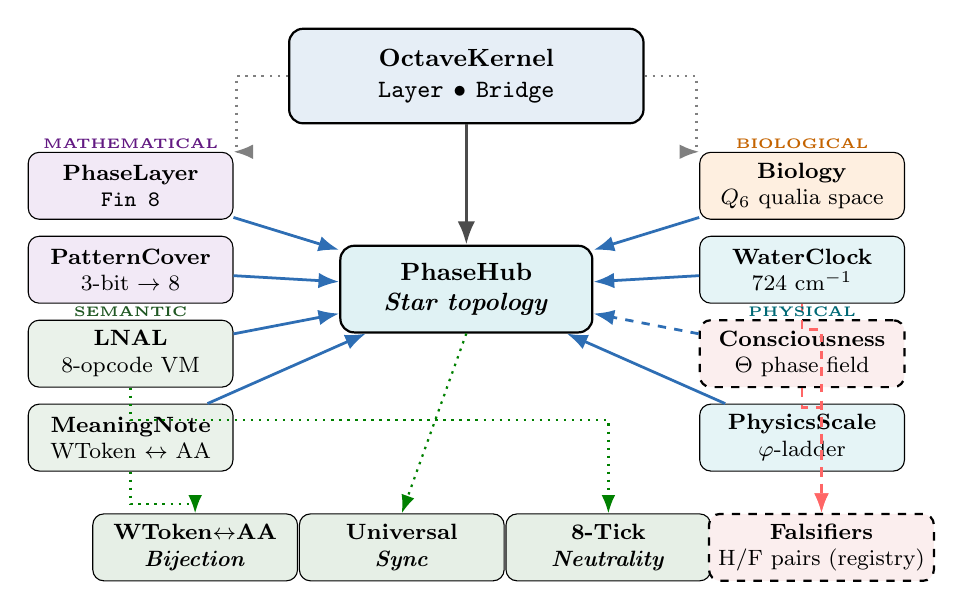
\begin{tikzpicture}[
  scale=0.82,
  box/.style={draw, rounded corners=4pt, minimum width=2.6cm, minimum height=0.85cm, 
              font=\footnotesize, align=center},
  core/.style={draw, rounded corners=5pt, minimum width=4.5cm, minimum height=1.2cm,
               fill=octBlue!12, thick, font=\small\bfseries, align=center},
  math/.style={box, fill=octPurple!10},
  semantic/.style={box, fill=octGreen!10},
  bio/.style={box, fill=octOrange!12},
  phys/.style={box, fill=octCyan!10},
  hub/.style={draw, rounded corners=5pt, minimum width=3.2cm, minimum height=1.1cm,
              fill=octCyan!12, thick, font=\small\bfseries, align=center},
  theorem/.style={box, fill=octGreen!12, font=\footnotesize\bfseries},
  empirical/.style={box, fill=octRed!8, dashed, thick},
  arrow/.style={oct/arrow},
  bridge/.style={oct/bridge}
]
  % Core abstraction
  \node[core] (kernel) at (0, 4) {
    \textbf{OctaveKernel}\\
    \texttt{Layer} $\bullet$ \texttt{Bridge}
  };
  
  % Mathematical Layers (left, top)
  \node[math] (phase) at (-5.2, 2.3) {
    \textbf{PhaseLayer}\\
    \texttt{Fin 8}
  };
  \node[math] (pattern) at (-5.2, 1) {
    \textbf{PatternCover}\\
    3-bit $\to$ 8
  };
  
  % Semantic Layers (left, bottom)
  \node[semantic] (lnal) at (-5.2, -0.3) {
    \textbf{LNAL}\\
    8-opcode VM
  };
  \node[semantic] (meaning) at (-5.2, -1.6) {
    \textbf{MeaningNote}\\
    WToken $\leftrightarrow$ AA
  };
  
  % Biological Layer (right, top)
  \node[bio] (biology) at (5.2, 2.3) {
    \textbf{Biology}\\
    $Q_6$ qualia space
  };
  
  % Physical Layers (right)
  \node[phys] (water) at (5.2, 1) {
    \textbf{WaterClock}\\
    724 cm$^{-1}$
  };
  \node[phys] (physics) at (5.2, -1.6) {
    \textbf{PhysicsScale}\\
    $\phival$-ladder
  };
  
  % Speculative Layer
  \node[empirical] (consciousness) at (5.2, -0.3) {
    \textbf{Consciousness}\\
    $\Theta$ phase field
  };
  
  % Bridge hub (center)
  \node[hub] (hub) at (0, 0.7) {
    \textbf{PhaseHub}\\
    \textit{Star topology}
  };
  
  % Key Theorems (bottom)
  \node[theorem] (bijection) at (-4.2, -3.3) {
    WToken$\leftrightarrow$AA\\
    \textit{Bijection}
  };
  \node[theorem] (sync) at (-1, -3.3) {
    Universal\\
    \textit{Sync}
  };
  \node[theorem] (neutral) at (2.2, -3.3) {
    8-Tick\\
    \textit{Neutrality}
  };
  
  % Falsifiers
  \node[empirical] (falsify) at (5.5, -3.3) {
    \textbf{Falsifiers}\\
    H/F pairs (registry)
  };
  
  % Arrows from core to hub
  \draw[arrow, very thick] (kernel) -- (hub);
  
  % Bridge arrows (layers to hub)
  \draw[bridge] (phase) -- (hub);
  \draw[bridge] (pattern) -- (hub);
  \draw[bridge] (lnal) -- (hub);
  \draw[bridge] (meaning) -- (hub);
  \draw[bridge] (biology) -- (hub);
  \draw[bridge] (water) -- (hub);
  \draw[bridge, dashed] (consciousness) -- (hub);
  \draw[bridge] (physics) -- (hub);
  
  % Instantiation arrows
  \draw[arrow, gray, dotted] (kernel.west) -- ++(-0.8, 0) |- (phase.north east);
  \draw[arrow, gray, dotted] (kernel.east) -- ++(0.8, 0) |- (biology.north west);
  
  % Theorem derivation arrows
  \draw[arrow, dotted, thick, green!50!black] (meaning.south) -- ++(0, -0.5) -| (bijection.north);
  \draw[arrow, dotted, thick, green!50!black] (hub.south) -- (sync.north);
  \draw[arrow, dotted, thick, green!50!black] (lnal.south) -- ++(0, -0.5) -| (neutral.north);
  
  % Falsifier connections
  \draw[arrow, red!60, dashed] (water.south) -- ++(0, -0.4) -| (falsify.north);
  \draw[arrow, red!60, dashed] (consciousness.south) -- ++(0, -0.3) -| (falsify.north);
  
  % Domain labels
  \node[font=\tiny\bfseries, octPurple!80!black] at (-5.2, 2.95) {MATHEMATICAL};
  \node[font=\tiny\bfseries, octGreen!70!black] at (-5.2, 0.35) {SEMANTIC};
  \node[font=\tiny\bfseries, octOrange!80!black] at (5.2, 2.95) {BIOLOGICAL};
  \node[font=\tiny\bfseries, octCyan!70!black] at (5.2, 0.35) {PHYSICAL};
  
  
\end{tikzpicture}
\caption{\textbf{Figure 1: The Octave System Architecture.} The core \texttt{OctaveKernel} abstraction (top) instantiates 8 concrete layers across four domains. All layers connect through the PhaseHub (center) via structure-preserving bridges (blue arrows). Derived results (green) are checked in the reference implementation; falsifiers (red dashed) specify refutation conditions for empirical hypotheses. Dashed elements indicate speculative components.}
\label{fig:overview}
\end{figure}

\subsubsection{The Bridge Network}

Layers connect through \emph{bridges}: typed maps between layers that preserve the \emph{shared} structure (phase and step). Concretely, a bridge $B : L_1 \to L_2$ is a state map with two requirements:
\begin{itemize}
  \item \textbf{Phase preservation}: $L_2.\phase(B(s)) = L_1.\phase(s)$.
  \item \textbf{Step commutation}: $L_2.\step(B(s)) = B(L_1.\step(s))$.
\end{itemize}

Intuitively, phase preservation says the two models agree on ``where they are in the 8-tick cycle,'' while step commutation says the map respects the dynamics (mapping-after-stepping equals stepping-after-mapping). Together, they guarantee:

\begin{theorem}[Phase Iteration, informal]
If layers $L_1$ and $L_2$ are connected by a bridge $B$, and both satisfy \StepAdvances{}, then for any starting state $s$ and any number of steps $n$:
\[
  L_2.\phase(L_2.\step^n(B(s))) = L_1.\phase(L_1.\step^n(s))
\]
\end{theorem}

In words: alignment is preserved under iteration; once two systems agree on phase (via a bridge), they keep agreeing as they evolve.

\paragraph{The PhaseHub Architecture.} Rather than connecting every layer to every other (requiring $\binom{8}{2} = 28$ bridges), we use a hub-and-spoke topology centered on \texttt{PhaseLayer}. Each domain layer projects to \texttt{PhaseLayer}; alignment between any two layers is then mediated through the hub. This reduces implementation complexity while preserving all theorems.

Our reference implementation includes explicit projection bridges (domain $\to$ PhaseLayer) and derived cross-domain bridges obtained by composing through the hub (see \S\ref{sec:bridge-network}).

\subsubsection{Built-In Falsifiability}

Every empirical hypothesis in our framework ships with an explicit \emph{falsifier}: a concrete experimental outcome that would count against the hypothesis. The goal is to prevent ``unfalsifiable'' claims and to prevent moving goalposts after data arrives.

\begin{example}[Cross-Octave Validation]
Consider the claim that better folding (lower RMSD) tends to correspond to higher audio consonance under a fixed sonification pipeline. We operationalize this as an \emph{order-consistency} test over a preregistered dataset: count how many pairs violate the expected ordering (lower RMSD but also lower consonance), and require that this count stay below a preregistered threshold $k$.

The paired falsifier is then simply: a preregistered dataset in which the number of such order violations exceeds $k$. By construction, the hypothesis and falsifier cannot both hold: if the falsifier condition is observed, the hypothesis is refuted.
\end{example}

This design requirement forces intellectual honesty: you cannot state a hypothesis without specifying how it could fail. The falsifier registry (\S\ref{sec:falsifiability}) records the hypothesis--falsifier pairs specified in the reference implementation, along with their intended tests and (where available) cited incompatibility proofs.

\subsubsection{Scale of Verification}

The conceptual framework is accompanied by a machine-checkable reference implementation. We report the following as \emph{audit metadata} (useful for reproducibility and review), not as evidence that the empirical hypotheses are true:

\begin{table}[H]
\centering
\begin{tabular}{ll}
\toprule
\textbf{Audit artifact} & \textbf{What it reports (scope + timestamp in file)} \\
\midrule
\texttt{artifacts/reality\_audit.json} & audit summary for a certificate surface (e.g., sorries/axioms under that scope) \\
\texttt{artifacts/sorry\_audit.json} & scan for \texttt{sorry} placeholders (code + documentation) \\
\texttt{artifacts/axiom\_audit.json} & explicit inventory of declared axioms (by file/category) \\
\texttt{artifacts/smuggling\_audit.json} & scan for degenerate proof-smuggling patterns (e.g.\ \texttt{∃\_, True}) \\
\bottomrule
\end{tabular}
\caption{Audit artifacts for reproducibility. We intentionally do not hard-code counts in the paper; audits may differ by scope.}
\label{tab:metrics}
\end{table}

The key takeaway is transparency: assumptions and remaining proof gaps are exposed by audit artifacts, and reviewers can independently inspect scope, timestamps, and results.

% ----------------------------------------------------------------------------
\subsection{What We Claim and What We Do Not}\label{sec:claims}

To prevent misunderstanding, we state explicitly what this paper claims and does not claim.

\subsubsection{What We Claim}

\begin{enumerate}
  \item \textbf{A precise framework exists}: The \texttt{OctaveKernel} abstraction defines a reusable interface for 8-phase dynamical models and their cross-domain connections.
  
  \item \textbf{Eight concrete instantiations are specified}: Each of the eight layers is defined against the same interface and carries an explicit epistemic status (proved/model/hypothesis/speculative).
  
  \item \textbf{Key results are proved within the framework}: The WToken--AminoAcid bijection (as a statement about the token system), the LNAL neutrality invariant, and the core synchronization lemma (pairwise alignment preservation, extended to finite families by pairwise application) are proved as formal theorems in the reference implementation.
  
  \item \textbf{Hypotheses have explicit falsifiers}: Every empirical claim comes with conditions for refutation.
  
  \item \textbf{The number 8 has mathematical origin}: The 3-bit pattern cover theorem derives the cycle length from combinatorics, not numerology.
\end{enumerate}

\subsubsection{What We Do Not Claim}

\begin{enumerate}
  \item \textbf{We do not claim the framework describes ultimate reality}. The Octave System is a \emph{model}---a formal structure that may or may not fit the world. Its value lies in being precise enough to test.
  
  \item \textbf{We do not claim all domains are unified}. Some layer instances are speculative (e.g., consciousness). Their inclusion demonstrates the framework's expressiveness, not their empirical validity.
  
  \item \textbf{We do not claim novelty for each component}. Many individual pieces (DFT, $\phival$-scaling, genetic code) are well-known. Our contribution is the \emph{integration} under a common verified structure.
  
  \item \textbf{We do not claim the hypotheses are confirmed}. They are \emph{proposed}. The framework's value is making them testable, not asserting their truth.
  
  \item \textbf{We do not claim 8 is metaphysically special}. It emerges from 3-bit combinatorics. Other pattern sizes would yield different cycle lengths.
\end{enumerate}

\subsubsection{The Epistemic Hierarchy}

Our claims form a hierarchy of certainty:

\begin{figure}[H]
\centering
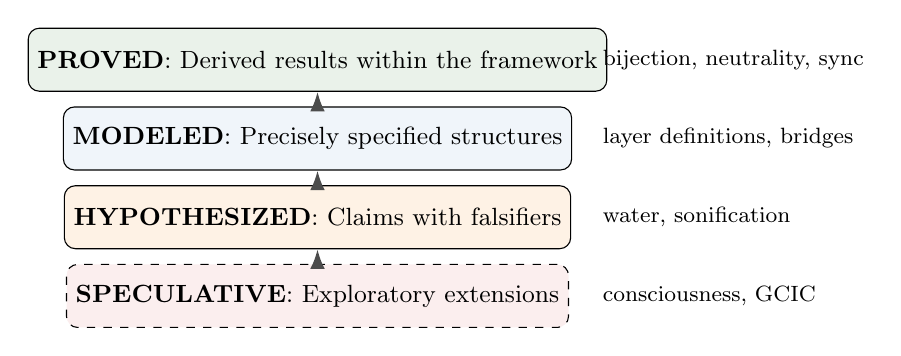
\begin{tikzpicture}[
  level/.style={draw, rounded corners, minimum width=6cm, minimum height=0.8cm, font=\small},
  arrow/.style={oct/arrow}
]
  \node[level, fill=octGreen!10] (proved) at (0, 3) {\textbf{PROVED}: Derived results within the framework};
  \node[level, fill=octBlue!7] (model) at (0, 2) {\textbf{MODELED}: Precisely specified structures};
  \node[level, fill=octOrange!10] (hyp) at (0, 1) {\textbf{HYPOTHESIZED}: Claims with falsifiers};
  \node[level, fill=octRed!8, dashed] (spec) at (0, 0) {\textbf{SPECULATIVE}: Exploratory extensions};
  
  \draw[arrow] (spec) -- (hyp);
  \draw[arrow] (hyp) -- (model);
  \draw[arrow] (model) -- (proved);
  
  \node[right, font=\footnotesize] at (3.5, 3) {bijection, neutrality, sync};
  \node[right, font=\footnotesize] at (3.5, 2) {layer definitions, bridges};
  \node[right, font=\footnotesize] at (3.5, 1) {water, sonification};
  \node[right, font=\footnotesize] at (3.5, 0) {consciousness, GCIC};
\end{tikzpicture}
\caption{Epistemic hierarchy of claims in the Octave System.}
\label{fig:epistemic}
\end{figure}

Every claim in this paper is tagged with its epistemic status. Readers can assess the certainty of each component independently.

% ----------------------------------------------------------------------------
\subsection{Main Results Preview}\label{sec:results-preview}

Before detailing the structure, we preview the three headline results. In this concept-first version we state them in plain language; formal statements and proofs are provided in the reference implementation.

\begin{theorem}[WToken--AminoAcid Bijection, \S\ref{sec:bijection}]
Within our 20-token semantic classification system (WTokens), there is an explicit one-to-one correspondence to the 20 standard amino acids.
\end{theorem}

This is a theorem about the token system we define. Any biochemical interpretation (e.g., post-hoc correspondences between token families and chemical properties) is discussed separately and is not required for the theorem.

\begin{theorem}[LNAL 8-Tick Neutrality, \S\ref{sec:neutrality}]
The LNAL semantic virtual machine satisfies an 8-tick conservation invariant: a ledger-like quantity balances to zero at the boundary of every 8-tick window.
\end{theorem}

Interpretation is domain-dependent; the proved content is the invariant itself.

\begin{theorem}[Universal Synchronization, \S\ref{sec:synchronization}]
If two 8-phase systems advance phase by one tick per step, then initial phase alignment between them is preserved under iteration (and thus extends to finite collections by pairwise application).
\end{theorem}

This is the central result: cross-domain synchronization is not assumed; it is a consequence of the shared interface (phase, step, and the \StepAdvances{} law).

% ----------------------------------------------------------------------------
\subsection{Paper Structure}\label{sec:structure}

The remainder of this paper is organized as follows:

\begin{description}
  \item[\S\ref{sec:kernel}] \textbf{The OctaveKernel Abstraction.} We define the \Layer{} structure with its five fields, introduce the key predicates (\StepAdvances{}, \texttt{PreservesAdmissible}, \texttt{NonincreasingCost}), and prove the 3-bit pattern cover theorem that derives the number 8 from combinatorics.
  
  \item[\S\ref{sec:instances}] \textbf{Concrete Layer Instances.} We present all eight domain instantiations:
  \begin{itemize}
    \item PhaseLayer (the reference clock)
    \item PatternCoverLayer (combinatorial origin)
    \item LNALBreathLayer (semantic virtual machine)
    \item MeaningNoteLayer (biosemiotics)
    \item BiologyQualiaLayer (protein folding)
    \item WaterClockLayer (molecular oscillator)
    \item ConsciousnessPhaseLayer (speculative)
    \item PhysicsScaleLayer ($\phival$-hierarchy)
  \end{itemize}
  Each includes state space, phase function, step function, and key properties.
  
  \item[\S\ref{sec:bridges}] \textbf{Bridge Network and Composition.} We define typed bridges, define bridge composition (and discuss associativity/unit laws), establish iteration theorems, and describe the PhaseHub star topology that reduces $O(n^2)$ connections to $O(n)$.
  
  \item[\S\ref{sec:theorems}] \textbf{Key Theorems.} We present our main results in full detail:
  \begin{enumerate}
    \item The WToken--AminoAcid bijection (with explicit mapping table)
    \item The LNAL 8-tick neutrality chain (with proof structure)
    \item The universal synchronization theorem (with concrete instantiation)
  \end{enumerate}
  
  \item[\S\ref{sec:falsifiability}] \textbf{Falsifiability Framework.} We define the hypothesis--falsifier structure, give worked examples, and provide a registry of the hypothesis--falsifier pairs in the reference implementation (including cited incompatibility proofs where available).
  
  \item[\S\ref{sec:related}] \textbf{Related Work.} We position our contribution against:
  \begin{itemize}
    \item Prior formalizations (Flyspeck, Feit-Thompson, Liquid Tensor)
    \item Category-theoretic approaches to physics
    \item Biosemiotics and code biology
    \item Consciousness theories (IIT, Orch-OR)
  \end{itemize}
  
  \item[\S\ref{sec:conclusion}] \textbf{Conclusion and Future Directions.} We summarize contributions, state the ``deeper claim'' (8-tick rhythm emerges from combinatorial necessity), and outline future work (additional layers, empirical validation, theoretical extensions).
\end{description}

\paragraph{Appendices.} The appendices provide:
\begin{itemize}
  \item Complete layer and bridge tables (Appendix~\ref{app:layer-table}, \ref{app:bridge-network})
  \item LNAL opcode semantics (Appendix~\ref{app:lnal-opcodes})
  \item Build instructions (Appendix~\ref{app:build})
  \item WToken classification (Appendix~\ref{app:wtoken})
  \item Detailed LNAL semantics (Appendix~\ref{app:lnal-semantics})
  \item Figures (Appendix~\ref{app:figures})
  \item Supplementary materials (Appendix~\ref{app:supplementary})
\end{itemize}

\paragraph{Reading Paths.} Depending on interest:
\begin{itemize}
  \item \textbf{Mathematicians}: Focus on \S\ref{sec:kernel}, \S\ref{sec:bridges}, \S\ref{sec:theorems}
  \item \textbf{Biologists}: Focus on \S\ref{sec:meaning-note-layer}, \S\ref{sec:biology-layer}, \S\ref{sec:bijection}
  \item \textbf{Computer Scientists}: Focus on \S\ref{sec:lnal-layer}, Appendix~\ref{app:lnal-semantics}
  \item \textbf{Philosophers of Science}: Focus on \S\ref{sec:claims}, \S\ref{sec:falsifiability}
  \item \textbf{Skeptics}: Start with \S\ref{sec:claims} (what we don't claim), then \S\ref{sec:falsifiability} (how to refute us)
\end{itemize}

% ============================================================================
% SECTION 2: THE OCTAVEKERNEL ABSTRACTION
% ============================================================================
\section{The OctaveKernel Abstraction}\label{sec:kernel}

This section presents the core structure of the Octave System as a reusable modeling interface. We introduce the basic ingredients (8-phase layers, bridges, and a small set of properties that make synchronization meaningful), and we explain why these ingredients are sufficient to reason about cross-domain alignment without smuggling in extra assumptions.

The guiding idea is to separate \emph{shared structure} from \emph{domain content}. Shared structure (phase, step, and bridge behavior) supports general theorems. Domain content (how a layer's state and cost relate to a real system) is treated as modeling or hypothesis and remains testable via explicit falsifiers.

% ============================================================================
% FIGURE 2: THE 8-TICK STRUCTURE (ENHANCED)
% ============================================================================
\begin{figure}[ht]
\centering
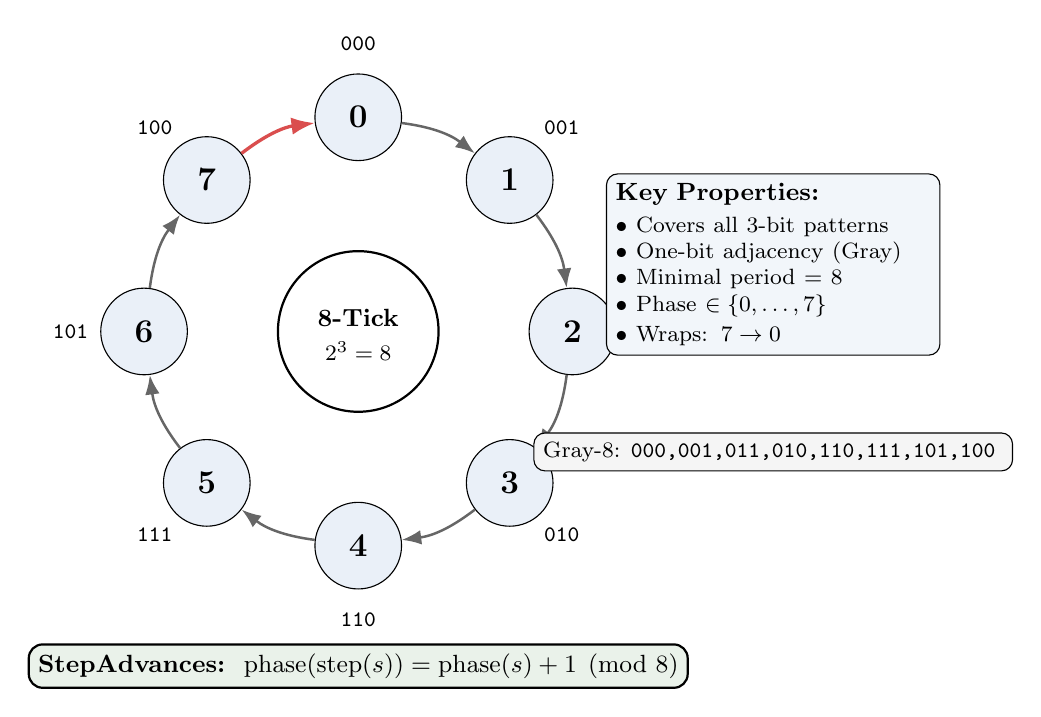
\begin{tikzpicture}[
  scale=0.85,
  phaseNode/.style={draw, circle, minimum size=1.1cm, fill=octBlue!10, font=\bfseries\large}
]
  % Main circle with 8 phases
  \def\radius{3.2}
  
  % Phase nodes: keep colors minimal and highlight the wrap arrow instead.
  \node[phaseNode] (p0) at (90:\radius) {0};
  \node[phaseNode] (p1) at (45:\radius) {1};
  \node[phaseNode] (p2) at (0:\radius) {2};
  \node[phaseNode] (p3) at (-45:\radius) {3};
  \node[phaseNode] (p4) at (-90:\radius) {4};
  \node[phaseNode] (p5) at (-135:\radius) {5};
  \node[phaseNode] (p6) at (180:\radius) {6};
  \node[phaseNode] (p7) at (135:\radius) {7};
  
  % Binary pattern labels (outside the circle)
  \node[font=\footnotesize\ttfamily, fill=white, rounded corners=2pt] at (90:4.3) {000};
  \node[font=\footnotesize\ttfamily, fill=white, rounded corners=2pt] at (45:4.3) {001};
  \node[font=\footnotesize\ttfamily, fill=white, rounded corners=2pt] at (0:4.3) {011};
  \node[font=\footnotesize\ttfamily, fill=white, rounded corners=2pt] at (-45:4.3) {010};
  \node[font=\footnotesize\ttfamily, fill=white, rounded corners=2pt] at (-90:4.3) {110};
  \node[font=\footnotesize\ttfamily, fill=white, rounded corners=2pt] at (-135:4.3) {111};
  \node[font=\footnotesize\ttfamily, fill=white, rounded corners=2pt] at (180:4.3) {101};
  \node[font=\footnotesize\ttfamily, fill=white, rounded corners=2pt] at (135:4.3) {100};
  
  % Arrows between consecutive phases (curved for better visualization)
  \draw[oct/arrow, draw=black!60] (p0) to[bend left=15] (p1);
  \draw[oct/arrow, draw=black!60] (p1) to[bend left=15] (p2);
  \draw[oct/arrow, draw=black!60] (p2) to[bend left=15] (p3);
  \draw[oct/arrow, draw=black!60] (p3) to[bend left=15] (p4);
  \draw[oct/arrow, draw=black!60] (p4) to[bend left=15] (p5);
  \draw[oct/arrow, draw=black!60] (p5) to[bend left=15] (p6);
  \draw[oct/arrow, draw=black!60] (p6) to[bend left=15] (p7);
  \draw[oct/arrow, draw=octRed!85, line width=1.2pt] (p7) to[bend left=15] (p0);
  
  % Center label with decorative circle
  \draw[fill=white, thick] (0,0) circle (1.2cm);
  \node[align=center, font=\small\bfseries] at (0, 0.2) {8-Tick};
  \node[align=center, font=\footnotesize] at (0, -0.3) {$2^3 = 8$};
  
  % Right side: Properties box (moved closer to avoid clipping)
  \node[draw, rounded corners, fill=octBlue!6, align=left, font=\small, text width=4cm] at (6.2, 1) {
    \textbf{Key Properties:}\\[2pt]
    \footnotesize
    $\bullet$ Covers all 3-bit patterns\\
    $\bullet$ One-bit adjacency (Gray)\\
    $\bullet$ Minimal period = 8\\
    $\bullet$ Phase $\in \{0,\ldots,7\}$\\
    $\bullet$ Wraps: $7 \to 0$
  };
  
  % Gray-8 witness (adjacent one-bit steps; ledger-compatible)
  \node[draw, rounded corners, fill=octGray, align=center, font=\footnotesize] at (6.2, -1.8) {
    Gray-8: \texttt{000,001,011,010,110,111,101,100}
  };
  
  % Bottom: The key equation (StepAdvances)
  \node[draw, rounded corners=5pt, fill=octGreen!10, font=\small, thick] at (0, -5) {
    \textbf{StepAdvances:} $\;\text{phase}(\text{step}(s)) = \text{phase}(s) + 1 \pmod{8}$
  };
  
\end{tikzpicture}
\caption{\textbf{Figure 2: The 8-Tick Cycle (Gray-8).} The fundamental phase cycle of the Octave System. Each phase (0--7) corresponds to a unique 3-bit pattern, arranged in Gray order so that consecutive phases differ in exactly one bit (including the wrap-around step). This realizes an 8-cycle on the 3-cube $Q_3$ that both covers all $2^3 = 8$ patterns and is compatible with one-coordinate ``atomic'' updates (Theorem~\ref{thm:period-8}). The \StepAdvances{} property (bottom) ensures each evolution step increments the phase by 1, with wrap-around from 7 to 0 (red arrow).}
\label{fig:8tick}
\end{figure}

% ----------------------------------------------------------------------------
\subsection{Layer Structure}\label{sec:layer-structure}

The fundamental building block of the Octave System is a \emph{layer}: a discrete-time model equipped with an explicit 8-phase clock. Layers are intentionally minimal---they capture only the structure needed to state cross-domain alignment and to attach costs/constraints when a domain calls for them.

\subsubsection{Motivation}

We want one interface that can describe very different kinds of models:
\begin{itemize}
  \item a minimal clock (state is just a phase $0\ldots7$),
  \item a complex machine state (many registers plus a phase),
  \item a sampled process (real-valued state with phase extracted from an observable),
  \item a constrained/optimized model (state plus admissibility constraints and a strain signal).
\end{itemize}
The commonality is not the domain content; it is the presence of a discrete rhythm and a one-tick update rule.

\subsubsection{Definition (conceptual)}

A layer $L$ consists of five components:
\begin{itemize}
  \item \textbf{State}: the domain-specific state space.
  \item \textbf{phase}: a projection $\texttt{State} \to \Fin{8}$ extracting the current phase.
  \item \textbf{step}: a one-tick update $\texttt{State} \to \texttt{State}$.
  \item \textbf{cost}: a strain/energy score $\texttt{State} \to \mathbb{R}$ (often constant $0$ when not used).
  \item \textbf{admissible}: a validity predicate $\texttt{State} \to \texttt{Prop}$ (often \texttt{True} when not used).
\end{itemize}
The first three define a clocked dynamical system. The last two support common scientific patterns: optimization (via cost) and invariants/constraints (via admissible).

\subsubsection{Field semantics (with examples)}

\paragraph{State.}
The state space can be small (e.g., just $\Fin{8}$) or large (e.g., a structured virtual-machine state or a real-valued vector). Examples in this paper include:
\begin{itemize}
  \item \textbf{PhaseLayer}: $\texttt{State}=\Fin{8}$.
  \item \textbf{LNALBreathLayer}: $\texttt{State}$ is a VM snapshot (registers, instruction pointer, etc.).
  \item \textbf{BiologyQualiaLayer}: $\texttt{State}$ is a folding/trajectory walker (position, tick, local strain).
  \item \textbf{PhysicsScaleLayer}: $\texttt{State}$ packages a scale index with a real-valued magnitude.
\end{itemize}

\paragraph{phase.}
Phase extraction is the key interoperability boundary: different domains compute phase differently, but all phases live in the same $\Fin{8}$. The only requirement is that phase is explicitly computable from state (no hidden or undecidable phase notion).

\paragraph{step.}
The step function is the model's one-tick evolution. Internally it can be arbitrarily complex; at the interface level it is simply ``advance by one tick.''

\paragraph{cost.}
Cost represents domain strain, energy, dissonance, or distance-to-target. Some layers use cost to model optimization pressure; others set it to a constant and ignore it.

\paragraph{admissible.}
Admissibility represents domain constraints (valid states). When used, admissibility is intended to be preserved by evolution; when not used, it can be set to \texttt{True}.

\subsubsection{Design rationale}

\paragraph{Why $\Fin{8}$ for phase?}
The canonical phase space comes from the combinatorial ``Why 8?'' argument (Section~\ref{sec:why-8}): an 8-step cycle is the minimal cyclic process that can enumerate all 3-bit contexts.

\paragraph{Why separate phase from step?}
Because we want to compare systems that are internally unrelated but share a rhythm. Separating phase extraction from the internal update rule lets the system remain conceptually small while still supporting complex domain models.

\paragraph{Why include cost and admissible in the interface?}
Because many domain models need (a) a notion of strain/fitness and/or (b) explicit constraints. Making these first-class fields keeps the interface uniform across domains.

\paragraph{Why not present everything categorically?}
Layers and bridges admit a natural category-style reading (layers as objects; bridges as structure-preserving morphisms). We keep the main presentation record-based for accessibility; the categorical viewpoint is optional and can be treated as an interpretation layer.

\subsubsection{Comparison to standard dynamical systems}

Standard dynamical systems often start from a state space $X$ and an update law (discrete $f:X\to X$ or continuous $\dot{x}=F(x)$). The Octave layer interface adds:
\begin{itemize}
  \item an explicit \textbf{discrete phase} $\Fin{8}$ (the common clock),
  \item an explicit \textbf{cost} (for optimization/strain reasoning),
  \item an explicit \textbf{admissibility predicate} (for invariants and constraints).
\end{itemize}
The discrete phase is what enables exact phase reasoning and (under additional conditions stated later) exact synchronization statements.

\subsubsection{Expressiveness}

The layer interface can represent a wide variety of models as long as an 8-phase component can be extracted. In this paper we use it to cover a range from combinatorial clocks to virtual machines to empirical/hypothesized oscillators.

% ----------------------------------------------------------------------------
\subsection{Layer Predicates}\label{sec:layer-predicates}

The layer interface becomes useful once we can state and reuse a small set of cross-cutting properties. We focus on three predicates:
\begin{itemize}
  \item \StepAdvances{} (the clock progresses deterministically),
  \item admissibility preservation (valid states stay valid), and
  \item cost non-increase (strain does not increase along evolution).
\end{itemize}
These are the minimal ingredients needed for (i) exact phase reasoning and (ii) standard invariant/optimization arguments.

\subsubsection{The StepAdvances Property}

\begin{definition}[StepAdvances]\label{def:step-advances}
A layer $L$ \emph{advances phase} if each step increments the phase by exactly $1$ (modulo $8$):
\[
  \forall s,\;\; L.\phase(L.\step(s)) = L.\phase(s) + 1 \pmod{8}.
\]
\end{definition}

This is the crucial property for synchronization. It ensures that:
\begin{enumerate}
  \item Every step makes progress (phase never stalls)
  \item Progress is uniform (always exactly +1, never +2 or +3)
  \item The cycle is predictable (phase after $n$ steps is $(p + n) \mod 8$)
\end{enumerate}

\begin{proposition}[Phase after $n$ steps]
If $L$ satisfies \StepAdvances{}, then for all $s$ and $n$:
\[
  L.\phase(L.\step^n(s)) = L.\phase(s) + n \pmod{8}
\]
\end{proposition}

\begin{proof}
Immediate by induction on $n$ using the defining equation for \StepAdvances{}.
\end{proof}

\subsubsection{Pairwise Alignment}

The main consequence of \StepAdvances{} is that phase-aligned layers remain aligned:

\begin{definition}[Aligned]\label{def:aligned}
Two states $s_1, s_2$ from layers $L_1, L_2$ are \emph{aligned} if they have the same phase:
\[
  \Aligned(L_1, L_2, s_1, s_2) \;:\!\iff\; L_1.\phase(s_1)=L_2.\phase(s_2).
\]
\end{definition}

\begin{theorem}[Pairwise Alignment Preservation]\label{thm:pairwise}
Let $L_1, L_2$ be layers satisfying \StepAdvances{}. If $\text{Aligned}(L_1, L_2, s_1, s_2)$, then for all $n \in \mathbb{N}$:
\[
  \text{Aligned}(L_1, L_2, L_1.\step^n(s_1), L_2.\step^n(s_2))
\]
\end{theorem}

\begin{proof}
This is a direct consequence of \StepAdvances{}: if both phases increment by $1$ each tick, equality of phases is preserved under iteration (formal proof by induction on $n$).
\end{proof}

\begin{corollary}[Eternal Synchronization]
If two layers start aligned and both satisfy \StepAdvances{}, they remain synchronized for all time---there is no drift, no phase slip, no desynchronization.
\end{corollary}

This is a \textbf{derived consequence of the interface}, not an empirical hypothesis: once the phase-advance law holds, alignment persistence follows mechanically.

\subsubsection{Triple and Universal Alignment}

The pairwise result extends to any finite collection:

\begin{theorem}[Universal Alignment Preservation]\label{thm:universal}
Let $L_1, \ldots, L_k$ be layers all satisfying \StepAdvances{}. If all pairs are initially aligned:
\[
  \forall i, j. \; L_i.\phase(s_i) = L_j.\phase(s_j)
\]
then after $n$ steps, all pairs remain aligned:
\[
  \forall i, j. \; L_i.\phase(L_i.\step^n(s_i)) = L_j.\phase(L_j.\step^n(s_j))
\]
\end{theorem}

\begin{proof}
Apply Theorem~\ref{thm:pairwise} to each pair $(L_i, L_j)$.
\end{proof}

\subsubsection{Admissibility Preservation}

\begin{definition}[PreservesAdmissible]\label{def:preserves-admissible}
A layer $L$ \emph{preserves admissibility} if valid states evolve to valid states:
\[
  \forall s,\;\; L.\admissible(s) \Rightarrow L.\admissible(L.\step(s)).
\]
\end{definition}

This is an invariant property: once established, it holds forever.

\begin{proposition}[Admissibility Induction]
If $L$ preserves admissibility and $L.\admissible(s)$, then $L.\admissible(L.\step^n(s))$ for all $n$.
\end{proposition}

\begin{proof}
By induction on $n$ using admissibility preservation at each step.
\end{proof}

\subsubsection{Cost Non-Increase}

\begin{definition}[NonincreasingCost]\label{def:nonincreasing-cost}
A layer $L$ has \emph{non-increasing cost} if evolution reduces (or preserves) cost on admissible states:
\[
  \forall s,\;\; L.\admissible(s) \Rightarrow L.\cost(L.\step(s)) \le L.\cost(s).
\]
\end{definition}

This property supports Lyapunov-style stability arguments:

\begin{proposition}[Cost Bound]
If $L$ satisfies \texttt{NonincreasingCost} and \texttt{PreservesAdmissible}, and $L.\admissible(s)$, then:
\[
  L.\cost(L.\step^n(s)) \leq L.\cost(s)
\]
for all $n$.
\end{proposition}

\begin{proof}
By iterating the one-step inequality and using admissibility preservation to ensure the premise holds at each step.
\end{proof}

\subsubsection{Predicate Summary}

\begin{table}[H]
\centering
\begin{tabular}{lll}
\toprule
\textbf{Predicate} & \textbf{Meaning} & \textbf{Consequence} \\
\midrule
\StepAdvances{} & Phase increments by 1 & Eternal synchronization \\
PreservesAdmissible & Valid $\to$ valid & Invariant preservation \\
NonincreasingCost & Cost decreases & Stability, convergence \\
\bottomrule
\end{tabular}
\caption{Summary of layer predicates.}
\end{table}

\textbf{Importance ranking}: \StepAdvances{} is essential for all synchronization theorems. PreservesAdmissible is required for layers with non-trivial invariants (e.g., LNAL). NonincreasingCost is optional but useful for optimization layers.

% ----------------------------------------------------------------------------
\subsection{Why 8? The Mathematical Origin}\label{sec:why-8}

The choice of an 8-phase clock is not musical or aesthetic. In the Octave System it is justified by a basic combinatorial minimality fact: if a process must cycle through all possible \emph{3-bit contexts}, then any cyclic schedule that ``covers'' all contexts has period at least $2^3 = 8$, and period $8$ is achievable.

\subsubsection{The pattern-cover question}

We model a 3-bit ``context'' as an element of the finite pattern space $\{0,1\}^3$ (equivalently, \texttt{Pattern 3} in our formal model). A cyclic schedule of period $p$ is simply a map
\[
  c : \Fin{p} \to \{0,1\}^3.
\]
We say $c$ is a \emph{cover} if it is surjective (every 3-bit pattern appears at some phase). The question is:
\emph{what is the smallest period $p$ for which such a cover exists?}

For the Octave System we take three binary features, so $|\{0,1\}^3| = 2^3 = 8$.

\subsubsection{The 3-Bit Case}

For binary alphabet $\Sigma = \{0, 1\}$ and $k = 3$, there are $2^3 = 8$ possible 3-bit patterns:

\begin{figure}[H]
\centering
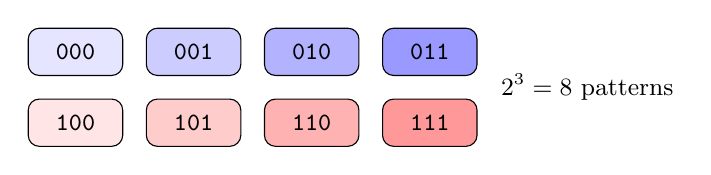
\begin{tikzpicture}[
  pattern/.style={draw, rounded corners, minimum width=1.2cm, minimum height=0.6cm, font=\ttfamily\small}
]
  % First row
  \node[pattern, fill=blue!10] at (0, 0) {000};
  \node[pattern, fill=blue!20] at (1.5, 0) {001};
  \node[pattern, fill=blue!30] at (3, 0) {010};
  \node[pattern, fill=blue!40] at (4.5, 0) {011};
  
  % Second row
  \node[pattern, fill=red!10] at (0, -0.9) {100};
  \node[pattern, fill=red!20] at (1.5, -0.9) {101};
  \node[pattern, fill=red!30] at (3, -0.9) {110};
  \node[pattern, fill=red!40] at (4.5, -0.9) {111};
  
  % Labels
  \node[font=\small] at (6.5, -0.45) {$2^3 = 8$ patterns};
\end{tikzpicture}
\caption{The eight 3-bit patterns.}
\end{figure}

\begin{theorem}[Pattern Cover Period (3-bit)]\label{thm:period-8}
Let $c : \Fin{p} \to \{0,1\}^3$ be a cyclic schedule. If $c$ is surjective (covers all 3-bit patterns), then $p \ge 8$. Moreover, there exists a schedule $c : \Fin{8} \to \{0,1\}^3$ that is bijective; in fact we can choose $c$ so that consecutive phases differ in exactly one bit (a Gray-8 cycle).
\end{theorem}

\begin{proof}
(\emph{Sketch}.) We prove both directions.

\textbf{Lower bound} ($p \geq 8$): If $c$ covers all 8 distinct 3-bit patterns, then a $p$-element domain must map onto an 8-element codomain, so necessarily $p \ge 8$.

\textbf{Upper bound} ($p \leq 8$): An explicit period-8 cover exists. One such choice (which also satisfies one-bit adjacency) is the Gray-8 order:
\[
  000 \to 001 \to 011 \to 010 \to 110 \to 111 \to 101 \to 100 \to 000.
\]
This visits all 8 patterns exactly once (so it is bijective), and each step flips exactly one bit. \qedhere
\end{proof}

\subsubsection{Reference implementation (formal check)}

A mechanically checked version of this argument exists in the reference implementation. In Lean:
(i) coverage is certified by the explicit Gray-8 witness (`IndisputableMonolith.Patterns.GrayCycle.grayCycle3_surjective`), and
(ii) one-bit adjacency is certified by `IndisputableMonolith.Patterns.GrayCycle.grayCycle3_oneBit_step`.
The OctaveKernel instance `IndisputableMonolith.OctaveKernel.Instances.PatternCover.patternAtPhase` uses this Gray-8 witness, and proves both surjectivity and one-bit adjacency (`patternAtPhase_surjective`, `patternAtPhase_oneBit_step`).

\subsubsection{Optional: window-cover via de Bruijn sequences}

If one insists on realizing a cover as sliding windows of a single cyclic string, de Bruijn sequences provide such witnesses. This is a different structure from Gray adjacency, so we treat it as an optional implementation detail rather than the canonical ``octave'' object.

\begin{theorem}[de Bruijn, 1946]
For any alphabet size $n$ and pattern length $k$, there exists a cyclic sequence of length $n^k$ containing every $k$-pattern exactly once.
\end{theorem}

For $(n, k) = (2, 3)$, this gives a length-$2^3 = 8$ cyclic string whose length-3 windows cover all 3-bit patterns. (This does \emph{not} imply one-bit adjacency between successive windows.)

\begin{table}[H]
\centering
\begin{tabular}{ccc}
\toprule
\textbf{Alphabet} & \textbf{Pattern length} & \textbf{Cycle period} \\
\midrule
$n = 2$ & $k = 1$ & $2^1 = 2$ \\
$n = 2$ & $k = 2$ & $2^2 = 4$ \\
$n = 2$ & $\mathbf{k = 3}$ & $\mathbf{2^3 = 8}$ \\
$n = 2$ & $k = 4$ & $2^4 = 16$ \\
$n = 3$ & $k = 2$ & $3^2 = 9$ \\
\bottomrule
\end{tabular}
\caption{De Bruijn sequence lengths for various $(n, k)$ (window-cover option).}
\end{table}

\subsubsection{Why 3-Bit Patterns?}

One might ask: why focus on 3-bit patterns rather than 2-bit or 4-bit?

\begin{enumerate}
  \item \textbf{Smallest nontrivial ``context''}: $k=3$ is the smallest window length that yields $2^k=8$ contexts (enough structure to be interesting while remaining simple).
  
  \item \textbf{A clear family of alternatives}: $k=2$ yields a 4-phase clock; $k=4$ yields a 16-phase clock. The Octave System focuses on the 8-phase case, but the underlying idea generalizes.
  
  \item \textbf{No claim of universality}: we do not claim all domains should be modeled with $k=3$. If a domain is better described by a different periodicity, the correct abstraction is a different $n^k$-phase interface.
\end{enumerate}

\subsubsection{Mathematical Origin, Not Mysticism}

This theorem is the \emph{mathematical origin} of the 8-tick structure. The number 8 arises because:

\begin{quote}
\textbf{Any system that must track, respond to, or cycle through all 3-bit configurations requires exactly 8 steps to complete one cycle.}
\end{quote}

This is a combinatorial minimality statement: the phase space $\Fin{8}$ is the smallest cyclic clock that can enumerate all 3-bit contexts without repetition.

\subsubsection{Connection to Music (Cautionary Note)}

The musical term ``octave'' (from Latin \emph{octavus}, ``eighth'') reflects that many Western pedagogical scales enumerate 8 note names before repeating (do--re--mi--fa--sol--la--ti--do). This numerical overlap is a naming convenience, not a derivation.

\begin{remark}[What We Do NOT Claim]
We do \emph{not} claim:
\begin{enumerate}
  \item That musical octaves (frequency ratio $2:1$) derive from the pattern cover theorem
  \item That the 8-note scale is mathematically ``necessary''
  \item That acoustics and combinatorics are deeply unified
\end{enumerate}
These would be empirical claims requiring evidence. We use ``octave'' as a memorable name, while remaining agnostic about deeper connections.
\end{remark}

\subsubsection{Implications for the Framework}

The pattern cover theorem has concrete implications:

\begin{enumerate}
  \item \textbf{Canonical phase space}: $\Fin{8}$ is the natural shared clock for 3-bit contexts.
  \item \textbf{Minimality}: fewer than 8 phases cannot cover all 3-bit windows in a cycle.
  \item \textbf{Sufficiency}: 8 phases are enough (a concrete cycle exists).
  \item \textbf{Modeling guidance}: when a domain's relevant context can be represented as three binary features, an 8-phase interface is a principled choice.
\end{enumerate}

\begin{figure}[H]
\centering
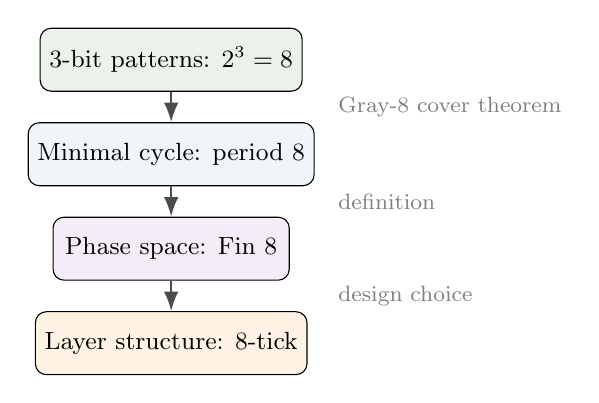
\begin{tikzpicture}[
  box/.style={draw, rounded corners, minimum width=3cm, minimum height=0.8cm, font=\small},
  arrow/.style={oct/arrow}
]
  \node[box, fill=octGreen!10] (math) at (0, 2) {3-bit patterns: $2^3 = 8$};
  \node[box, fill=octBlue!7] (cycle) at (0, 0.8) {Minimal cycle: period 8};
  \node[box, fill=octPurple!8] (phase) at (0, -0.4) {Phase space: $\Fin{8}$};
  \node[box, fill=octOrange!10] (layer) at (0, -1.6) {Layer structure: 8-tick};
  
  \draw[arrow] (math) -- (cycle);
  \draw[arrow] (cycle) -- (phase);
  \draw[arrow] (phase) -- (layer);
  
  \node[right, font=\footnotesize, gray] at (2, 1.4) {Gray-8 cover theorem};
  \node[right, font=\footnotesize, gray] at (2, 0.2) {definition};
  \node[right, font=\footnotesize, gray] at (2, -1) {design choice};
\end{tikzpicture}
\caption{Derivation chain from combinatorics to layer structure.}
\end{figure}

% ============================================================================
% SECTION 3: CONCRETE LAYER INSTANCES
% ============================================================================
\section{Concrete Layer Instances}\label{sec:instances}

We now instantiate the layer interface across eight domains. The goal of this section is not to argue that all domains are equally well-established; it is to show that the \emph{same} interface can accommodate:
\begin{itemize}
  \item purely mathematical constructions (where everything is definitional),
  \item designed computational models (where invariants can be stated and checked), and
  \item empirically anchored hypotheses (where falsifiers specify what would refute the claim).
\end{itemize}
Across all cases, the common comparison surface is the 8-phase clock and the one-tick evolution rule; any additional domain interpretation is explicitly labeled as model, hypothesis, or speculation.

\subsection{Overview of the Eight Layers}\label{sec:layer-overview}

The eight layers below range from abstract to concrete, and from established to speculative:

\begin{table}[H]
\centering
\small
\begin{tabular}{clllc}
\toprule
\textbf{\#} & \textbf{Layer} & \textbf{Domain} & \textbf{State Space} & \textbf{Status} \\
\midrule
1 & PhaseLayer & Pure math & $\Fin{8}$ & Trivial \\
2 & PatternCoverLayer & Combinatorics & $\Fin{8}$ & Proved \\
3 & LNALBreathLayer & Semantics & VM state (11 registers) & Proved \\
4 & MeaningNoteLayer & Biosemiotics & WToken bundles & Proved \\
5 & BiologyQualiaLayer & Protein folding & $Q_6$ trajectories & Model \\
6 & WaterClockLayer & Biophysics & Oscillator state & Hypothesis \\
7 & ConsciousnessPhaseLayer & Consciousness & Phase field & Speculative \\
8 & PhysicsScaleLayer & Scale physics & $\phival$-ladder & Model \\
\bottomrule
\end{tabular}
\caption{Overview of the eight concrete layer instances.}
\label{tab:layer-overview}
\end{table}

\paragraph{Epistemic Status Key:}
\begin{itemize}
  \item \textbf{Trivial}: a minimal construction used as a reference (properties hold by design).
  \item \textbf{Proved}: the key interface properties used later (e.g., phase-advance and stated invariants) are established within the framework.
  \item \textbf{Model}: a precise structure intended as an abstraction of domain behavior; empirical fit is an external question.
  \item \textbf{Hypothesis}: includes empirical commitments paired with explicit falsifiers.
  \item \textbf{Speculative}: exploratory extension included to demonstrate expressiveness; not presented as established science.
\end{itemize}

\paragraph{Reading This Section.} Each layer subsection follows a consistent format:
\begin{enumerate}
  \item \textbf{Motivation}: Why this layer exists
  \item \textbf{State space}: What constitutes a state
  \item \textbf{Definition (conceptual)}: How phase and step are defined (formal details in the reference implementation)
  \item \textbf{Key properties}: Which interface predicates it satisfies and why that matters
  \item \textbf{Hypotheses/Falsifiers}: For empirical commitments, what would refute them
\end{enumerate}

% ----------------------------------------------------------------------------
\subsection{PhaseLayer: The Reference Clock}\label{sec:phase-layer}

\subsubsection{Motivation}

Every framework needs a shared reference. \texttt{PhaseLayer} is the simplest possible layer: its state \emph{is} the phase. It serves three roles:
\begin{enumerate}
  \item a \textbf{canonical reference} for defining alignment (``same phase''),
  \item a \textbf{hub} for cross-domain comparison (other layers project to it), and
  \item a \textbf{sanity check} for the interface (if the reference clock fails, nothing else can be trusted).
\end{enumerate}

\subsubsection{State Space}

The state space is simply $\Fin{8} = \{0, 1, 2, 3, 4, 5, 6, 7\}$.

\subsubsection{Definition (conceptual)}

PhaseLayer is the ``pure clock'':
\begin{itemize}
  \item \textbf{phase}(s) is just $s$ itself (identity),
  \item \textbf{step}(s) increments by $1$ modulo $8$,
  \item \textbf{cost} is constantly $0$, and
  \item \textbf{admissible} is always true.
\end{itemize}
Formal details are provided in the reference implementation.

\subsubsection{Properties}

\begin{proposition}[PhaseLayer satisfies all predicates]
\texttt{PhaseLayer} satisfies \StepAdvances{}, \texttt{PreservesAdmissible}, and \texttt{NonincreasingCost}.
\end{proposition}

\begin{proof}
All are immediate from the definitions: phase advances by one tick, admissibility is always true, and cost is constant.
\end{proof}

\subsubsection{Role in the Framework}

\texttt{PhaseLayer} acts as the shared comparison surface: each domain layer provides a projection to phase, and cross-domain alignment is phrased in terms of equality in $\Fin{8}$. This enables the PhaseHub architecture (\S\ref{sec:phase-hub}): instead of connecting every pair of domains directly, we connect each domain to the hub and reason through that common reference.

% ----------------------------------------------------------------------------
\subsection{PatternCoverLayer: The Combinatorial Origin}\label{sec:pattern-cover-layer}

\subsubsection{Motivation}

This layer is the most direct bridge between the abstract interface and its combinatorial origin. It makes the ``Why 8?'' argument concrete: the phase index is interpreted as a position in a period-8 \emph{Gray-8} pattern-cover cycle (Figure~\ref{fig:8tick}, Theorem~\ref{thm:period-8}).

\subsubsection{State Space}

In the reference implementation, the witness layer is intentionally minimal: the state is just the phase itself:
\[
  \texttt{State} = \Fin{8}.
\]
A separate \emph{observation} function interprets each phase as a 3-bit pattern on the Gray-8 cycle (\texttt{patternAtPhase} in the reference implementation). If one wants an unbounded ``time'' counter for logging or traces, it can be added as an auxiliary field without changing the phase/step theorems, but it is not part of the certified core witness.

\subsubsection{Definition (conceptual)}

The definitions mirror the intended meaning:
\begin{itemize}
  \item \textbf{phase} returns the pattern index (an element of $\Fin{8}$),
  \item \textbf{step} increments the phase index (mod 8),
  \item \textbf{cost} is constantly $0$ (this layer is not an optimization model), and
  \item \textbf{admissible} is always true.
\end{itemize}

\subsubsection{Properties}

By construction, this layer satisfies \StepAdvances{}: stepping advances the phase index by exactly one tick (modulo 8).

\subsubsection{Connection to the Gray-8 witness}

The reference implementation attaches the combinatorial content through an explicit observation map
\[
  \texttt{patternAtPhase} : \Fin{8} \to \{0,1\}^3,
\]
which is bijective (complete cover) and satisfies one-bit adjacency between successive phases (Gray adjacency). Concretely, the Gray-8 correspondence used throughout the paper is:

\begin{table}[H]
\centering
\begin{tabular}{ccc}
\toprule
\textbf{Phase} & \textbf{3-bit pattern (Gray)} & \textbf{Binary value} \\
\midrule
0 & 000 & 0 \\
1 & 001 & 1 \\
2 & 011 & 3 \\
3 & 010 & 2 \\
4 & 110 & 6 \\
5 & 111 & 7 \\
6 & 101 & 5 \\
7 & 100 & 4 \\
\bottomrule
\end{tabular}
\caption{Phase-to-pattern correspondence in PatternCoverLayer (Gray-8).}
\end{table}

This layer is the most explicit ``combinatorial clock'' in the system: it provides a concrete interpretation of the abstract phase index as a traversal of all 3-bit contexts in a minimal cycle. Other layers may adopt the same 8-phase interface for different reasons, but this layer shows the interface is not arbitrary. (De Bruijn sequences provide an alternative \emph{window-cover} construction; we treat that as optional and distinct from Gray adjacency, as discussed in Section~\ref{sec:why-8}.)

% ----------------------------------------------------------------------------
\subsection{LNALBreathLayer: Semantic Virtual Machine}\label{sec:lnal-layer}

\subsubsection{Motivation}

The \LNAL{} (Light Native Assembly Language) is a minimal virtual machine intended as a \emph{worked example} of a domain layer with nontrivial internal state, explicit invariants, and an 8-tick ledger-style conservation property. Unlike a conventional VM optimized for throughput, LNAL is designed to make cross-cutting structure easy to state:
\begin{enumerate}
  \item \textbf{Phase alignment}: Every operation respects the 8-tick cycle
  \item \textbf{Conservation}: a ledger-like quantity balances over 8 ticks (an invariant, not a metaphor)
  \item \textbf{Symmetry}: Operations come in complementary pairs
\end{enumerate}

\subsubsection{Architecture Overview}

\begin{table}[H]
\centering
\begin{tabular}{ll}
\toprule
\textbf{Component} & \textbf{Specification} \\
\midrule
Opcodes & 8: LOCK, BALANCE, FOLD, SEED, BRAID, MERGE, LISTEN, FLIP \\
Primary registers & 6 (Reg6): $\nu_\phi$, $\ell$, $\sigma$, $\tau$, $k_\perp$, $\phi_E$ \\
Auxiliary registers & 5 (Aux5): neighborSum, tokenCt, hydrationS, phaseLock, freeSlot \\
Breath cycle & 1024 ticks (FLIP at tick 512) \\
Window size & 8 ticks \\
\bottomrule
\end{tabular}
\caption{LNAL architecture summary.}
\end{table}

\subsubsection{State Space}

Conceptually, an LNAL state contains:
\begin{itemize}
  \item a small set of primary and auxiliary registers,
  \item a breath counter (position in a longer ``breath'' cycle),
  \item control state (instruction pointer, halted flag, memory), and
  \item an 8-tick window tracker used for a ledger/invariant.
\end{itemize}
Phase is extracted from the breath counter modulo 8. The full state record is given in the reference implementation; we omit the full listing here.

\subsubsection{The 8 Opcodes}

\begin{table}[H]
\centering
\small
\begin{tabular}{lllc}
\toprule
\textbf{Opcode} & \textbf{Effect} & \textbf{Pair} & \textbf{Cost} \\
\midrule
LOCK & Set phaseLock := true & (unlocks via timeout) & 1 \\
BALANCE & Adjust tokenCt (inc/dec/reset/cycle) & self-paired & 1 \\
FOLD & Propagate phase, update signature & SEED & 2 \\
SEED & Initialize pattern & FOLD & 1 \\
BRAID & Weave with neighbor state & MERGE & 2 \\
MERGE & Combine register values & BRAID & 1 \\
LISTEN & No-op (await external input) & FLIP & 0 \\
FLIP & Invert state at breath midpoint & LISTEN & 0 \\
\bottomrule
\end{tabular}
\caption{LNAL opcodes with costs.}
\end{table}

\subsubsection{Key Invariants}

In the reference implementation, we separate two layers of structure:
\begin{itemize}
  \item \textbf{OctaveKernel layer witness (conservative)}: the LNALBreathLayer instance is packaged with \texttt{cost := 0} and \texttt{admissible := True}. This witness is used to certify the \emph{8-beat phase clock} and its one-tick advancement under VM stepping.
  \item \textbf{VM invariants (separate theorems)}: nontrivial properties of the VM (e.g., the 8-tick neutrality/reset behavior of \texttt{winSum8}) are stated and proved as separate theorems about LNAL semantics under explicit invariants such as \texttt{EightTickInvariant}.
\end{itemize}
This split is deliberate: it prevents us from smuggling empirical or program-dependent assumptions into the kernel layer interface while still allowing strong, checkable invariants to be proved about the VM.

\subsubsection{Definition (conceptual)}

The layer is parameterized by a program $P$:
\begin{itemize}
  \item \textbf{State}: VM state snapshot.
  \item \textbf{phase}: breath-counter modulo 8.
  \item \textbf{step}: one VM tick (fetch/decode/execute/update).
  \item \textbf{cost}: $0$ (conservative witness; costs/instruction models live outside the kernel layer witness).
  \item \textbf{admissible}: \texttt{True} (conservative witness; VM invariants are stated separately).
\end{itemize}
Different programs yield different instances but share the same 8-phase interface.

\subsubsection{Properties}

For the reference implementation, the key interface properties are established: stepping advances phase by one tick (via the breath counter), and the layer predicates \texttt{PreservesAdmissible} / \texttt{NonincreasingCost} hold trivially for this conservative witness. The nontrivial content (the neutrality/reset behavior) is provided by the separate theorems in the neutrality chain below.

\subsubsection{The 8-Tick Neutrality Chain}

The key theorem about LNAL is the \emph{neutrality chain}: over every 8-tick window, the ``ledger'' balances.

\begin{theorem}[8-Tick Neutrality]\label{thm:lnal-neutrality}
At the boundary of each 8-tick window, a ledger-like accumulator returns to zero.
\end{theorem}

Interpretation depends on how LNAL is used. The proved content is the invariant itself (a conservation-style statement over fixed windows). Formal statements and proofs are provided in the reference implementation and the detailed semantics appendix.

% ----------------------------------------------------------------------------
\subsection{MeaningNoteLayer: Semantic-Biological Bridge}\label{sec:meaning-note-layer}

\subsubsection{Motivation}

This layer packages a structured 20-token ``semantic alphabet'' (WTokens) and relates it to the 20 standard amino acids. In the framework, the rigorous claim is about the \emph{token system we define}: it has exactly 20 well-formed tokens and admits an explicit one-to-one mapping to the 20 amino-acid symbols. Any further interpretation of this correspondence (as biology, meaning, or mechanism) is kept separate and treated as modeling or hypothesis.

\subsubsection{WToken Classification}

WTokens are classified by three discrete parameters:
\begin{itemize}
  \item a DFT-8 mode family (four families),
  \item a $\phival$-level (four levels), and
  \item a $\tau$-offset (used only in one special family).
\end{itemize}
The well-formedness constraint is simply that $\tau$-offset variants are only allowed for the designated family; this yields a controlled, finite token set rather than an arbitrary Cartesian product.

\subsubsection{The 20-Token Counting}

\begin{table}[H]
\centering
\begin{tabular}{lccc}
\toprule
\textbf{Mode Family} & \textbf{$\phival$-levels} & \textbf{$\tau$-offsets} & \textbf{Count} \\
\midrule
(1+7) & 4 & 1 & 4 \\
(2+6) & 4 & 1 & 4 \\
(3+5) & 4 & 1 & 4 \\
(4) & 4 & 2 & 8 \\
\midrule
\textbf{Total} & & & \textbf{20} \\
\bottomrule
\end{tabular}
\caption{WToken counting: 4 + 4 + 4 + 8 = 20.}
\end{table}

\subsubsection{State Space}

Conceptually, a \texttt{MeaningNote} bundles:
\begin{itemize}
  \item a WToken (one semantic atom),
  \item an amino acid (one biochemical atom),
  \item a representative codon, and
  \item the requirement that the codon decodes to that amino acid under the genetic code model.
\end{itemize}
We omit the full record definition in this concept-first paper.

\subsubsection{The Bijection Theorem}

\begin{theorem}[WToken--AminoAcid Bijection]\label{thm:bijection-def}
There exists an explicit one-to-one correspondence between the 20 well-formed WTokens and the 20 standard amino acids.
\end{theorem}

This is a theorem about the token system as defined. It does \emph{not} by itself establish a biological mechanism; it establishes that our semantic classification admits an exact 20-way alignment with the amino-acid alphabet.

\subsubsection{Layer Definition}

The layer itself cycles through meaning-notes on an 8-tick schedule (phase extracted from a tick counter modulo 8). Cost and admissibility encode simple well-formedness and bookkeeping. Formal details are provided in the reference implementation.

\subsubsection{Semantic-Chemical Correspondences}

Beyond the existence of the bijection, one can inspect qualitative correspondences between token families and coarse chemical classes. These are \emph{interpretive observations} about the chosen token naming/classification and are not required for the core theorem.

\begin{table}[H]
\centering
\small
\begin{tabular}{lll}
\toprule
\textbf{Semantic Property} & \textbf{Chemical Property} & \textbf{Preserved?} \\
\midrule
Mode (1+7): Ground tokens & Small/hydrophobic amino acids & Yes \\
Mode (2+6): Relational tokens & Polar, uncharged amino acids (Ser, Thr, Asn, Gln) & Yes \\
Mode (3+5): Interactive tokens & Charged residues (Asp, Glu, Lys, Arg) & Yes \\
Mode (4): Central/structural tokens & Aromatic + special structural residues & Yes \\
$\phival$-level 0: Simplest & Smallest side chain & Yes \\
\bottomrule
\end{tabular}
\caption{Notable semantic-chemical correspondences.}
\end{table}

These correspondences are \emph{observed post-hoc}, not assumed. The bijection exists independently of whether these qualitative labels are the ``right'' way to talk about amino-acid chemistry.

% ----------------------------------------------------------------------------
\subsection{MeaningNoteLayer: Semantic-Biological Bridge}\label{sec:meaning-note-layer}

This layer formalizes the correspondence between semantic atoms and biochemistry.

\begin{definition}[MeaningNote]
\begin{lstlisting}
structure MeaningNote where
  wtoken : WTokenSpec
  amino : AminoAcid
  codon : Codon
  decodes : genetic_code codon = .amino amino
\end{lstlisting}
\end{definition}

A \texttt{MeaningNote} bundles:
\begin{itemize}
  \item A \emph{WToken}: one of 20 semantic atoms classified by DFT-8 mode
  \item An \emph{AminoAcid}: one of 20 biological building blocks
  \item A \emph{Codon}: a representative DNA triplet
  \item A proof that the codon decodes to the amino acid
\end{itemize}

The WToken classification produces exactly 20 tokens:
\begin{itemize}
  \item 4 mode families: $(1+7), (2+6), (3+5), (4)$
  \item 4 $\phival$-levels: 0, 1, 2, 3
  \item Mode-4 has $\tau$-offset variants
  \item Total: $4 \times 4 + 4 = 20$
\end{itemize}

This matches the 20 amino acids exactly---a correspondence we prove as a bijection (Theorem~\ref{thm:bijection}).

% ============================================================================
% FIGURE 4: WTOKEN-AMINOACID BIJECTION (ENHANCED)
% ============================================================================
\begin{figure}[ht]
\centering
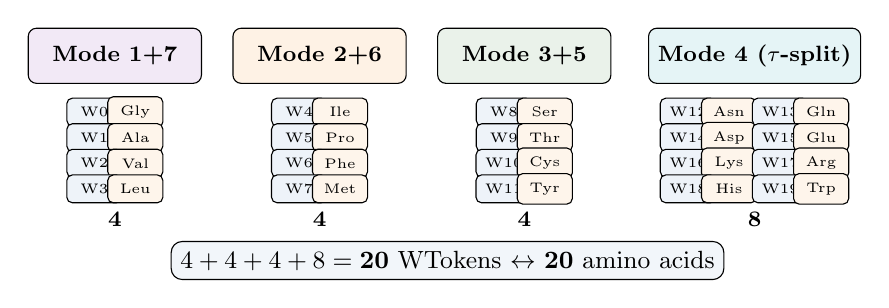
\begin{tikzpicture}[scale=0.65,
  mode/.style={draw, rounded corners=3pt, minimum width=2.2cm, minimum height=0.7cm, 
               font=\footnotesize\bfseries, align=center},
  token/.style={draw, rectangle, rounded corners=2pt, minimum width=0.7cm, 
                minimum height=0.35cm, font=\tiny, fill=octBlue!8},
  amino/.style={draw, rectangle, rounded corners=2pt, minimum width=0.7cm, 
                minimum height=0.35cm, font=\tiny, fill=octOrange!8}
]
  % Mode families (simplified headers)
  \node[mode, fill=octPurple!10] (m17) at (0, 3.5) {Mode 1+7};
  \node[mode, fill=octOrange!10] (m26) at (4, 3.5) {Mode 2+6};
  \node[mode, fill=octGreen!10] (m35) at (8, 3.5) {Mode 3+5};
  \node[mode, fill=octCyan!10] (m4) at (12.5, 3.5) {Mode 4 ($\tau$-split)};
  
  % Mode 1+7 tokens (compact)
  \node[token] at (-0.4, 2.4) {W0}; \node[amino] at (0.4, 2.4) {Gly};
  \node[token] at (-0.4, 1.9) {W1}; \node[amino] at (0.4, 1.9) {Ala};
  \node[token] at (-0.4, 1.4) {W2}; \node[amino] at (0.4, 1.4) {Val};
  \node[token] at (-0.4, 0.9) {W3}; \node[amino] at (0.4, 0.9) {Leu};
  
  % Mode 2+6 tokens
  \node[token] at (3.6, 2.4) {W4}; \node[amino] at (4.4, 2.4) {Ile};
  \node[token] at (3.6, 1.9) {W5}; \node[amino] at (4.4, 1.9) {Pro};
  \node[token] at (3.6, 1.4) {W6}; \node[amino] at (4.4, 1.4) {Phe};
  \node[token] at (3.6, 0.9) {W7}; \node[amino] at (4.4, 0.9) {Met};
  
  % Mode 3+5 tokens
  \node[token] at (7.6, 2.4) {W8}; \node[amino] at (8.4, 2.4) {Ser};
  \node[token] at (7.6, 1.9) {W9}; \node[amino] at (8.4, 1.9) {Thr};
  \node[token] at (7.6, 1.4) {W10}; \node[amino] at (8.4, 1.4) {Cys};
  \node[token] at (7.6, 0.9) {W11}; \node[amino] at (8.4, 0.9) {Tyr};
  
  % Mode 4 tokens (8 total in two columns)
  \node[token] at (11.2, 2.4) {W12}; \node[amino] at (12, 2.4) {Asn};
  \node[token] at (11.2, 1.9) {W14}; \node[amino] at (12, 1.9) {Asp};
  \node[token] at (11.2, 1.4) {W16}; \node[amino] at (12, 1.4) {Lys};
  \node[token] at (11.2, 0.9) {W18}; \node[amino] at (12, 0.9) {His};
  \node[token] at (13, 2.4) {W13}; \node[amino] at (13.8, 2.4) {Gln};
  \node[token] at (13, 1.9) {W15}; \node[amino] at (13.8, 1.9) {Glu};
  \node[token] at (13, 1.4) {W17}; \node[amino] at (13.8, 1.4) {Arg};
  \node[token] at (13, 0.9) {W19}; \node[amino] at (13.8, 0.9) {Trp};
  
  % Counts
  \node[font=\footnotesize\bfseries] at (0, 0.3) {4};
  \node[font=\footnotesize\bfseries] at (4, 0.3) {4};
  \node[font=\footnotesize\bfseries] at (8, 0.3) {4};
  \node[font=\footnotesize\bfseries] at (12.5, 0.3) {8};
  
  % Formula
  \node[draw, rounded corners=4pt, fill=octBlue!6, font=\small] at (6.5, -0.5) {
    $4 + 4 + 4 + 8 = \mathbf{20}$ WTokens $\leftrightarrow$ \textbf{20} amino acids
  };
  
\end{tikzpicture}
\caption{\textbf{Figure 4: WToken--AminoAcid Bijection.} The 20 WTokens, classified by DFT-8 mode family (columns), $\phival$-level (rows 0--3), and $\tau$-offset (mode 4 only), map bijectively to the 20 standard amino acids. Mode (4) is self-conjugate and allows two phase variants ($\tau_0$, $\tau_2$), doubling its token count to 8. This correspondence is a \textbf{proved theorem} (constructive bijection with explicit inverse), not a hypothesis.}
\label{fig:bijection}
\end{figure}

% ----------------------------------------------------------------------------
\subsection{BiologyQualiaLayer: Protein Folding}\label{sec:biology-layer}

\subsubsection{Motivation}

Protein folding---the process by which a linear amino acid chain finds its 3D structure---is a central problem in computational biology. This layer models folding as trajectory optimization in a discrete space.

\subsubsection{The $Q_6$ Qualia Hypercube}

\begin{definition}[$Q_6$ Qualia Hypercube]
The space $Q_6$ is the 6-dimensional Boolean hypercube $\{0,1\}^6$, with:
\begin{itemize}
  \item \textbf{64 vertices}: Each corresponds to a codon (DNA triplet)
  \item \textbf{Edges}: Connect vertices differing in exactly one coordinate (single-nucleotide mutations)
  \item \textbf{Hamming distance}: $d(v_1, v_2) = |\{i : v_1^i \neq v_2^i\}|$
\end{itemize}
\end{definition}

The $Q_6$ structure captures the combinatorial topology of the genetic code: nearby vertices represent codons that can mutate into each other.

\begin{figure}[H]
\centering
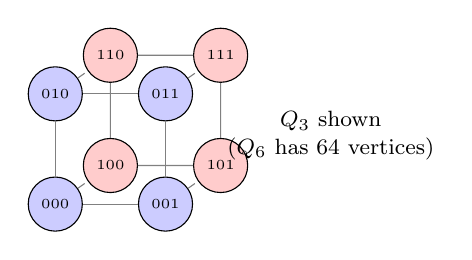
\begin{tikzpicture}[scale=0.7]
  % Simplified Q_6 visualization (show 3D projection)
  \node[draw, circle, fill=blue!20, minimum size=0.6cm, font=\tiny] (000) at (0, 0) {000};
  \node[draw, circle, fill=blue!20, minimum size=0.6cm, font=\tiny] (001) at (2, 0) {001};
  \node[draw, circle, fill=blue!20, minimum size=0.6cm, font=\tiny] (010) at (0, 2) {010};
  \node[draw, circle, fill=blue!20, minimum size=0.6cm, font=\tiny] (011) at (2, 2) {011};
  \node[draw, circle, fill=red!20, minimum size=0.6cm, font=\tiny] (100) at (1, 0.7) {100};
  \node[draw, circle, fill=red!20, minimum size=0.6cm, font=\tiny] (101) at (3, 0.7) {101};
  \node[draw, circle, fill=red!20, minimum size=0.6cm, font=\tiny] (110) at (1, 2.7) {110};
  \node[draw, circle, fill=red!20, minimum size=0.6cm, font=\tiny] (111) at (3, 2.7) {111};
  
  \draw[gray] (000) -- (001) -- (011) -- (010) -- (000);
  \draw[gray] (100) -- (101) -- (111) -- (110) -- (100);
  \draw[gray, dashed] (000) -- (100);
  \draw[gray, dashed] (001) -- (101);
  \draw[gray, dashed] (010) -- (110);
  \draw[gray, dashed] (011) -- (111);
  
  \node[font=\footnotesize] at (5, 1.5) {$Q_3$ shown};
  \node[font=\footnotesize] at (5, 1) {($Q_6$ has 64 vertices)};
\end{tikzpicture}
\caption{The 3-dimensional hypercube $Q_3$ (for illustration). $Q_6$ has $2^6 = 64$ vertices.}
\end{figure}

\subsubsection{State Space}

\begin{definition}[Trajectory-walker state (conceptual)]
A state represents a ``walker'' moving through a discrete trajectory while tracking a scalar strain:
\begin{itemize}
  \item \textbf{trajectory}: a finite sequence of codon indices (states in the $Q_6$ proxy),
  \item \textbf{position}: the current index into that sequence,
  \item \textbf{tick}: an abstract time counter, and
  \item \textbf{localStrain}: a real-valued deviation score (lower is ``better'' under the model).
\end{itemize}
\end{definition}

\subsubsection{Layer Definition}

The BiologyQualiaLayer instantiates the 8-phase interface as follows:
\begin{itemize}
  \item \textbf{State}: a trajectory-walker state.
  \item \textbf{phase}: \texttt{tick mod 8}.
  \item \textbf{step}: advance the walker by one tick (and update position/strain as specified by the model).
  \item \textbf{cost}: \texttt{localStrain} (a strain proxy).
  \item \textbf{admissible}: \texttt{True} in the conservative witness layer (trajectory bounds are carried in the state as proof fields).
\end{itemize}
We omit the full formal definition in this concept-first paper.

\subsubsection{Properties}

\begin{proposition}
BiologyQualiaLayer satisfies \StepAdvances{}.
\end{proposition}

Intuitively, stepping increments the tick, so the phase advances by one modulo 8.

\subsubsection{Hypothesis and Falsifier}

\begin{hypothesis}[H\_FoldingRhythm: 8-Tick Folding Rhythm]
Protein folding dynamics exhibit an 8-tick rhythm aligned with water molecular clocks. Specifically, folding intermediates show spectral peaks at frequencies related to 724~cm$^{-1}$ / 8.
\end{hypothesis}

\begin{falsifier}{F\_NoFoldingRhythm}
Time-resolved folding measurements (e.g., ultrafast IR spectroscopy) show no spectral peak at the predicted frequency ($\pm 5\%$).
\end{falsifier}

In the framework, hypotheses are paired with explicit falsifiers of this kind; the formal encoding ensures the hypothesis and falsifier cannot both hold for the same dataset by construction (the logical negation is part of the specification).
In the reference implementation, some hypothesis/falsifier pairs are formalized over typed data schemas, and their incompatibility can then be proved and machine-checked. Where a pair is only specified here at the protocol level (not yet formalized in Lean), incompatibility checking should be treated as future work (see \S\ref{sec:falsifiability}).

% ----------------------------------------------------------------------------
\subsection{WaterClockLayer: Physical Oscillator}\label{sec:water-layer}

\subsubsection{Motivation}

This layer connects the abstract 8-tick structure to a concrete physical phenomenon: the vibrational dynamics of water's hydrogen-bond network. Unlike the purely mathematical layers, this one makes empirical predictions.

\subsubsection{The 724~cm$^{-1}$ Water Libration Band}

Water exhibits a strong infrared absorption band at approximately 724~cm$^{-1}$ (wavenumber), corresponding to:
\begin{itemize}
  \item \textbf{Frequency}: $\nu \approx 2.17 \times 10^{13}$~Hz
  \item \textbf{Period}: $T \approx 46$~fs (femtoseconds)
  \item \textbf{Physical origin}: Hindered rotations (librations) of water molecules within the hydrogen-bond network
\end{itemize}

This is an established empirical fact from infrared spectroscopy \cite{water_spectroscopy}.

\subsubsection{The 8-Fold Sub-Structure Hypothesis}

\begin{hypothesis}[H\_WaterLibration: 8-Fold Band Structure]
The 724~cm$^{-1}$ band exhibits fine structure with 8 coherent sub-bands, spaced by approximately 724/8 $\approx$ 90.5~cm$^{-1}$.
\end{hypothesis}

\begin{falsifier}{F\_NoBandStructure}
High-resolution IR spectroscopy (resolution $< 1$~cm$^{-1}$) shows no coherent 8-fold sub-band structure in the 700--750~cm$^{-1}$ region.
\end{falsifier}

In practice this is instantiated as a preregistered detection criterion (e.g., ``eight coherent sub-bands around 724~cm$^{-1}$'' under an explicit coherence threshold); the falsifier is its negation on the same dataset.

\subsubsection{The $\tau$-Gate Timing Hypothesis}

\begin{hypothesis}[H\_TauGate: Fundamental Timing Reference]
The fundamental timing reference for biological coherence is $\tau_\text{gate} \approx 65$~ps, derived from water network dynamics.
\end{hypothesis}

\begin{falsifier}{F\_TauGateMismatch}
Ultrafast spectroscopy measurements of water relaxation timescales differ from 65~ps by more than 20~ps.
\end{falsifier}

\paragraph{Physical interpretation.} The $\tau$-gate represents the timescale on which water's hydrogen-bond network can ``gate'' (allow or block) coherent energy transfer between molecular sites.

\subsubsection{State Space}

\begin{definition}[Water-clock state (conceptual)]
A water-clock observation/state records:
\begin{itemize}
  \item \textbf{band index}: which of the 8 sub-bands (0--7) is active/dominant under the analysis,
  \item \textbf{signal-to-noise}: a scalar SNR estimate for the band structure,
  \item \textbf{correlation}: a cross-band coherence/correlation measure,
  \item \textbf{phase dispersion}: a circular-variance style summary, and
  \item \textbf{temperature}: measurement temperature (defaulting to 277~K in the model).
\end{itemize}
\end{definition}

\subsubsection{Layer Definition}

The WaterClockLayer instantiates the interface as:
\begin{itemize}
  \item \textbf{phase}: the current sub-band index (0--7),
  \item \textbf{step}: advance to the next sub-band (a model of cycling through an 8-fold structure),
  \item \textbf{cost}: lower is ``better'' (e.g., $1-\mathrm{SNR}$ in one simple scoring model), and
  \item \textbf{admissible}: basic data-quality constraints (e.g., positive SNR and sufficiently high cross-band correlation).
\end{itemize}
We omit the full real-valued record and formal layer definition here.

\subsubsection{Properties}

\begin{proposition}
WaterClockLayer satisfies \StepAdvances{}.
\end{proposition}

Intuitively, the step cycles the sub-band index in $\Fin{8}$, so phase advances by one per tick.

\subsubsection{Temperature Dependence}

One discriminating prediction is temperature dependence: if an 8-fold coherent sub-structure exists, it should exhibit a reproducible temperature profile rather than appearing arbitrarily.

\begin{hypothesis}[H\_TemperaturePeak]
The 8-fold coherence peaks at $T = 277$~K ($\pm 1$~K).
\end{hypothesis}

\begin{falsifier}{F\_WrongTemperature}
Coherence peaks at a temperature differing from 277~K by more than 2~K.
\end{falsifier}

% ----------------------------------------------------------------------------
\subsection{ConsciousnessPhaseLayer: Mind Clock}\label{sec:consciousness-layer}

\subsubsection{Epistemic Warning}

\begin{quote}
\textbf{This is the most speculative layer.} We include it not to make definitive claims about consciousness, but to demonstrate:
\begin{enumerate}
  \item The \Layer{} abstraction is expressive enough for radical hypotheses
  \item Speculation can be made \emph{honest} through explicit falsifiers
  \item The framework distinguishes proved theorems from exploratory extensions
\end{enumerate}
\end{quote}

Readers uncomfortable with speculation may skip this subsection without losing the paper's main contributions.

\subsubsection{Motivation}

The ``hard problem of consciousness'' asks how physical processes give rise to subjective experience. We do not solve this problem. Instead, we include one deliberately speculative extension to illustrate how the framework treats ambitious claims: it forces explicit definitions, separates mechanism from interface, and pairs every hypothesis with a falsifier.

\subsubsection{The Global Co-Identity Constraint (GCIC)}

\begin{hypothesis}[H\_GCIC: Global Co-Identity Constraint]
All conscious observers share a universal phase field $\Theta \in [0, 2\pi)$. This field advances uniformly, providing a common timing reference for subjective reports.
\end{hypothesis}

\begin{falsifier}{F\_LocalPhases}
Experiments with spatially separated observers show persistent, irreconcilable phase differences in their reported subjective timing that cannot be attributed to signal delays.
\end{falsifier}

\textbf{How to test (example sketch)}: define an operational proxy for ``subjective timing'' (e.g., a behavioral timing task with physiological recording) and check whether geographically separated observers admit a consistent phase alignment after controlling for signal delay and known confounders. (This subsection is illustrative; it does not prescribe a finalized experimental design.)

\subsubsection{The 45-Tick Mind Clock}

\begin{hypothesis}[H\_45TickMindClock]
Subjective time has a 45-tick period. One motivation is that a longer internal cycle can still project to the 8-phase interface while providing additional structure; the number 45 is proposed here via a $\phival$-motivated heuristic:
\[
  45 = 8 \times 5 + 5 \approx 8 \times \phival^3
\]
where $\phival^3 \approx 4.236$.
\end{hypothesis}

\begin{falsifier}{F\_WrongMindClockPeriod}
Psychophysical measurements of subjective timing granularity show a period other than 45 (relative to an established physiological reference).
\end{falsifier}

\subsubsection{State Space}

Conceptually, a consciousness-state record for this toy layer would include:
\begin{itemize}
  \item a global phase $\Theta$ (intended to lie in $[0,2\pi)$),
  \item a discrete 45-tick counter (as a ``mind clock''),
  \item an internal coherence score, and
  \item a recognition/clarity score (used here as a cost proxy).
\end{itemize}
We omit the full real-valued record definition.

\subsubsection{Layer Definition}

The conceptual layer instance is:
\begin{itemize}
  \item \textbf{phase}: the 45-tick counter projected modulo 8,
  \item \textbf{step}: increment the counter and advance $\Theta$ uniformly,
  \item \textbf{cost}: a simple function of coherence and recognition/clarity, and
  \item \textbf{admissible}: basic bounds (e.g., coherence above a threshold and $\Theta$ within a chosen interval).
\end{itemize}
The key point is that a longer internal cycle can still expose an 8-phase interface via projection.

\subsubsection{Properties}

\begin{proposition}
ConsciousnessPhaseLayer satisfies \StepAdvances{}.
\end{proposition}

Intuitively, stepping increments the internal tick, so the projected phase advances by one modulo 8.

\subsubsection{Relationship to Established Theories}

\begin{table}[H]
\centering
\small
\begin{tabular}{lll}
\toprule
\textbf{Theory} & \textbf{Claim} & \textbf{Our Relation} \\
\midrule
IIT \cite{tononi2016integrated} & Consciousness = $\Phi$ & We don't compute $\Phi$ \\
Orch-OR \cite{penrose1994shadows} & Quantum collapse in microtubules & We're agnostic on mechanism \\
Global Workspace \cite{baars1988cognitive} & Broadcast to workspace & Compatible with GCIC \\
\bottomrule
\end{tabular}
\caption{Relationship to existing consciousness theories.}
\end{table}

We neither endorse nor refute these theories. Our contribution is providing a \emph{formal, falsifiable} structure that could be tested.

% ----------------------------------------------------------------------------
\subsection{PhysicsScaleLayer: $\phival$-Ladder}\label{sec:physics-layer}

\subsubsection{Motivation}

Physical phenomena span enormous scale ranges---from Planck length ($10^{-35}$~m) to cosmic horizons ($10^{26}$~m). This layer formalizes the hypothesis that scales cluster on ``rungs'' separated by powers of $\phival$.

\subsubsection{The $\phival$-Ladder Hypothesis}

\begin{hypothesis}[H\_PhiLadderPeriodicity]
Physical scales cluster on rungs separated by factors of $\phival \approx 1.618$. The structure repeats every 8 rungs, giving a ratio of $\phival^8 \approx 46.98$ per ``octave.''
\end{hypothesis}

\begin{falsifier}{F\_NoPhiClustering}
Statistical analysis of physical constants shows no significant clustering at $\phival$-spaced intervals (compared to random spacing).
\end{falsifier}

\subsubsection{State Space}

Conceptually, a state in this layer records:
\begin{itemize}
  \item a rung index (position on a putative ladder),
  \item a representative scale value (e.g., a log-scale summary),
  \item a coupling strength (a bounded proxy for cross-scale interaction), and
  \item an 8-phase index indicating position within an 8-rung ``octave''.
\end{itemize}

\subsubsection{Layer Definition}

The PhysicsScaleLayer instantiates the interface as:
\begin{itemize}
  \item \textbf{phase}: the 8-rung position (either stored explicitly or derived from rung modulo 8),
  \item \textbf{step}: advance one rung (and update the representative scale accordingly under the model),
  \item \textbf{cost}: lower is ``better'' (e.g., higher coupling corresponds to lower cost), and
  \item \textbf{admissible}: basic bounds on any real-valued proxies (e.g., coupling in $[0,1]$).
\end{itemize}
We omit the full real-valued record and formal definition in this concept-first paper.

\subsubsection{Cross-Scale Coupling}

\begin{hypothesis}[H\_RungCoupling]
Cross-scale coupling decays as $\phival^{-\Delta\text{rung}}$. Phenomena separated by $\Delta$ rungs interact with strength proportional to $\phival^{-\Delta}$.
\end{hypothesis}

\begin{falsifier}{F\_RungCouplingMismatch}
Measured cross-scale coupling between physical phenomena does not follow $\phival^{-\Delta}$ decay (deviates by more than 20\% from prediction).
\end{falsifier}

\subsubsection{Example: Scale Hierarchy}

\begin{table}[H]
\centering
\small
\begin{tabular}{clcl}
\toprule
\textbf{Rung} & \textbf{Scale} & \textbf{$\log_{10}$} & \textbf{Phenomenon} \\
\midrule
0 & Planck & $-35$ & Quantum gravity \\
8 & $\phival^8 \times$ Planck & $-33.3$ & String scale? \\
16 & $\phival^{16} \times$ Planck & $-31.6$ & GUT scale \\
... & ... & ... & ... \\
$n$ & Nuclear & $-15$ & Strong force \\
$n+8$ & Atomic & $-10$ & Chemistry \\
$n+16$ & Cellular & $-5$ & Biology \\
\bottomrule
\end{tabular}
\caption{Hypothetical $\phival$-ladder scale hierarchy.}
\end{table}

\subsubsection{Properties}

\begin{proposition}
PhysicsScaleLayer satisfies \StepAdvances{}.
\end{proposition}

Intuitively, stepping advances the rung by one, hence the 8-phase index advances by one modulo 8.

% ----------------------------------------------------------------------------
\subsection{Layer Summary}\label{sec:layer-summary}

\begin{table}[H]
\centering
\small
\begin{tabular}{lcccc}
\toprule
\textbf{Layer} & \textbf{StepAdv} & \textbf{PresAdm} & \textbf{NonincCost} & \textbf{Hypotheses} \\
\midrule
PhaseLayer & \checkmark & \checkmark & \checkmark & 0 \\
PatternCoverLayer & \checkmark & \checkmark & \checkmark & 0 \\
LNALBreathLayer & \checkmark & \checkmark & -- & 0 \\
MeaningNoteLayer & \checkmark & \checkmark & -- & 0 \\
BiologyQualiaLayer & \checkmark & -- & \checkmark & 1 \\
WaterClockLayer & \checkmark & -- & \checkmark & 3 \\
ConsciousnessPhaseLayer & \checkmark & -- & -- & 2 \\
PhysicsScaleLayer & \checkmark & \checkmark & \checkmark & 2 \\
\midrule
\textbf{Total} & 8/8 & 6/8 & 5/8 & 8 \\
\bottomrule
\end{tabular}
\caption{Summary of layer properties. All 8 layers satisfy \StepAdvances{}; fewer satisfy the optional predicates.}
\end{table}

% ============================================================================
% SECTION 4: BRIDGE NETWORK AND COMPOSITION
% ============================================================================
\section{Bridge Network and Composition}\label{sec:bridges}

\subsection{Motivation: Connecting Domains}\label{sec:bridge-motivation}

Layers in isolation describe individual domains. But the Octave System's power emerges when we ask: \emph{How do different domains relate?} 

Consider these questions:
\begin{itemize}
  \item If a semantic pattern (WToken) is at phase 3, what is the corresponding physical state (water clock)?
  \item Does evolving in the biology domain for 8 steps give the same phase as evolving in the physics domain?
  \item Can we ``translate'' between consciousness and chemistry without losing phase information?
\end{itemize}

\textbf{Bridges} answer these questions by providing structure-preserving maps between layers. Here, ``structure'' means two explicit requirements: (i) the map preserves 8-phase alignment, and (ii) it commutes with the step dynamics.

\subsection{Bridge Structure}\label{sec:bridge-structure}

\subsubsection{The Definition}

\begin{definition}[Bridge]\label{def:bridge}
A \emph{bridge} between layers $L_1$ and $L_2$ consists of a state-translation map $B.\map : L_1.\State \to L_2.\State$ satisfying two laws:
\begin{align*}
  L_2.\phase(B.\map(s)) &= L_1.\phase(s) && \text{(phase preservation)} \\
  L_2.\step(B.\map(s)) &= B.\map(L_1.\step(s)) && \text{(step commutation)}
\end{align*}
\end{definition}

\subsubsection{Component Analysis}

\begin{table}[H]
\centering
\begin{tabular}{lll}
\toprule
\textbf{Component} & \textbf{Type} & \textbf{Meaning} \\
\midrule
\texttt{map} & $L_1.\text{State} \to L_2.\text{State}$ & State translation \\
\texttt{preservesPhase} & $\forall s, L_2.\phase(\map(s)) = L_1.\phase(s)$ & Phase coherence \\
\texttt{commutesStep} & $\forall s, L_2.\step(\map(s)) = \map(L_1.\step(s))$ & Dynamics compatibility \\
\bottomrule
\end{tabular}
\caption{Bridge components.}
\end{table}

\paragraph{Intuition.}
\begin{itemize}
  \item \texttt{map}: The ``dictionary'' translating $L_1$-states to $L_2$-states.
  \item \texttt{preservesPhase}: Translation doesn't shift the clock. A state at phase 5 in $L_1$ maps to a state at phase 5 in $L_2$.
  \item \texttt{commutesStep}: It doesn't matter whether we step then map, or map then step---we arrive at the same place.
\end{itemize}

\subsubsection{Commutative Diagram}

The \texttt{commutesStep} property is captured by the following commutative diagram:

\begin{figure}[H]
\centering
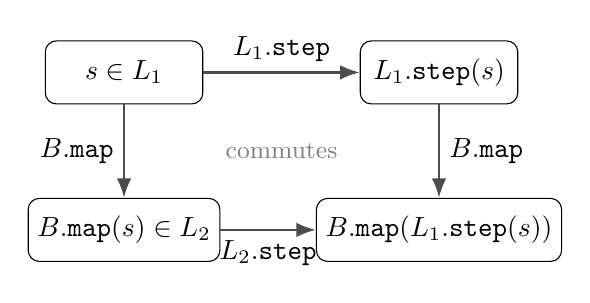
\begin{tikzpicture}[
  state/.style={draw, rounded corners, minimum width=2cm, minimum height=0.8cm},
  arrow/.style={oct/arrow}
]
  \node[state] (s1) at (0, 2) {$s \in L_1$};
  \node[state] (s1') at (4, 2) {$L_1.\step(s)$};
  \node[state] (s2) at (0, 0) {$B.\map(s) \in L_2$};
  \node[state] (s2') at (4, 0) {$B.\map(L_1.\step(s))$};
  
  \draw[arrow] (s1) -- node[above] {$L_1.\step$} (s1');
  \draw[arrow] (s1) -- node[left] {$B.\map$} (s2);
  \draw[arrow] (s1') -- node[right] {$B.\map$} (s2');
  \draw[arrow] (s2) -- node[below] {$L_2.\step$} (s2');
  
  \node[font=\small, gray] at (2, 1) {commutes};
\end{tikzpicture}
\caption{Bridge commutativity: the diagram commutes, meaning both paths from top-left to bottom-right yield the same result.}
\end{figure}

\subsubsection{Why Typed Bridges?}

We could simply use bare functions $L_1.\State \to L_2.\State$. But requiring the two bridge laws above provides practical guarantees:

\begin{enumerate}
  \item \textbf{Checkable correctness}: a proposed bridge either satisfies phase preservation and step commutation, or it does not.
  \item \textbf{Composability}: bridges can be chained without losing the two invariants (see \S\ref{sec:bridge-composition}).
  \item \textbf{Network reasoning}: once bridges are lawful, we can reason about the behavior of entire translation networks (e.g., long-run alignment under iteration).
  \item \textbf{Explicit failure modes}: if a candidate translation breaks phase or dynamics, the failure is visible rather than implicit.
\end{enumerate}

\subsubsection{What Bridges Do NOT Guarantee}

\begin{itemize}
  \item \textbf{Cost preservation}: A bridge may map low-cost states to high-cost states.
  \item \textbf{Admissibility preservation}: A valid state in $L_1$ may map to an invalid state in $L_2$.
  \item \textbf{Bijectivity}: Bridges are not required to be invertible.
\end{itemize}

We could add these as optional properties, but the core definition is intentionally minimal.

\subsection{The Identity Bridge}\label{sec:bridge-identity}

Every layer has an identity bridge to itself:

\begin{definition}[Identity Bridge]
For any layer $L$, the identity bridge $\Bridge.\text{id}(L)$ uses $\map(s)=s$ and satisfies both bridge laws immediately:
\[
  L.\phase(\map(s)) = L.\phase(s)
  \qquad\text{and}\qquad
  L.\step(\map(s)) = \map(L.\step(s)).
\]
\end{definition}

\begin{proposition}
$\Bridge.\text{id}(L)$ satisfies both bridge axioms trivially.
\end{proposition}

\subsection{Composition Theorem}\label{sec:bridge-composition}

\subsubsection{Statement and Proof}

Bridges compose to form new bridges---this is the key enabling theorem for the PhaseHub architecture.

\begin{theorem}[Bridge Composition]\label{thm:bridge-comp}
Given bridges $B_1 : \Bridge(L_1, L_2)$ and $B_2 : \Bridge(L_2, L_3)$, there exists a bridge $B_1 \then B_2 : \Bridge(L_1, L_3)$.
\end{theorem}

The composite bridge uses the composite map:
\[
  (B_1 \then B_2).\map \;:=\; B_2.\map \circ B_1.\map.
\]

\begin{proof}
For \texttt{preservesPhase}:
\[
  L_3.\phase((B_2.\map \circ B_1.\map)(s)) = L_3.\phase(B_2.\map(B_1.\map(s))) \stackrel{B_2}{=} L_2.\phase(B_1.\map(s)) \stackrel{B_1}{=} L_1.\phase(s)
\]

For \texttt{commutesStep}, we show the diagram commutes:
\begin{align*}
  L_3.\step((B_2.\map \circ B_1.\map)(s)) &= L_3.\step(B_2.\map(B_1.\map(s))) \\
  &= B_2.\map(L_2.\step(B_1.\map(s))) \quad \text{($B_2$ commutes)} \\
  &= B_2.\map(B_1.\map(L_1.\step(s))) \quad \text{($B_1$ commutes)} \\
  &= (B_2.\map \circ B_1.\map)(L_1.\step(s)) \qedhere
\end{align*}
\end{proof}

\subsubsection{Associativity}

Composition is associative, enabling chain constructions:

\begin{theorem}[Composition Associativity]\label{thm:bridge-assoc}
For bridges $B_1 : \Bridge(L_1, L_2)$, $B_2 : \Bridge(L_2, L_3)$, $B_3 : \Bridge(L_3, L_4)$:
\[
  (B_1 \then B_2) \then B_3 = B_1 \then (B_2 \then B_3)
\]
\end{theorem}

\begin{proof}
Both sides have map $B_3.\map \circ B_2.\map \circ B_1.\map$. The proof obligations reduce to function composition associativity.
\end{proof}

\subsubsection{Unit Laws}

The identity bridge acts as a left and right unit:

\begin{proposition}[Identity Laws]
\begin{align*}
  \Bridge.\text{id}(L_1) \then B &= B \\
  B \then \Bridge.\text{id}(L_2) &= B
\end{align*}
\end{proposition}

\subsubsection{Category-Theoretic Interpretation}

These results establish that bridges form a \emph{category}:

\begin{proposition}[The Category $\mathbf{Lay}_8$]
Define a category $\mathbf{Lay}_8$ where:
\begin{itemize}
  \item \textbf{Objects}: \Layer{} instances
  \item \textbf{Morphisms}: Bridges
  \item \textbf{Identity}: $\Bridge.\text{id}(L)$
  \item \textbf{Composition}: $\Bridge.\comp$
\end{itemize}
This satisfies the category axioms (identity laws and associativity).
\end{proposition}

We do not develop category theory further here; the categorical reading is optional and mainly serves as a compact way to remember the laws.

\subsection{Iteration Theorems}\label{sec:bridge-iteration}

The bridge properties extend from single steps to arbitrary iteration. This is crucial for long-term synchronization.

\subsubsection{Phase Iteration}

\begin{theorem}[Phase Iteration]\label{thm:phase-iterate}
For any bridge $B : \Bridge(L_1, L_2)$ and $n \in \mathbb{N}$:
\[
  L_2.\phase(L_2.\step^n(B.\map(s))) = L_1.\phase(L_1.\step^n(s))
\]
\end{theorem}

\begin{proof}
This follows by induction on $n$ using the bridge laws (phase preservation and step commutation). A fully formal proof is given in the reference implementation.
\end{proof}

\subsubsection{Map Iteration}

\begin{theorem}[Map Iteration]\label{thm:map-iterate}
For any bridge $B : \Bridge(L_1, L_2)$ and $n \in \mathbb{N}$:
\[
  L_2.\step^n(B.\map(s)) = B.\map(L_1.\step^n(s))
\]
\end{theorem}

This theorem states that \textbf{bridges commute with time}:

\begin{figure}[H]
\centering
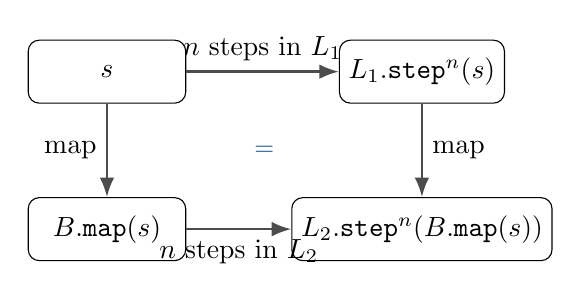
\begin{tikzpicture}[
  state/.style={draw, rounded corners, minimum width=2cm, minimum height=0.8cm},
  arrow/.style={oct/arrow}
]
  \node[state] (s1) at (0, 2) {$s$};
  \node[state] (s1n) at (4, 2) {$L_1.\step^n(s)$};
  \node[state] (s2) at (0, 0) {$B.\map(s)$};
  \node[state] (s2n) at (4, 0) {$L_2.\step^n(B.\map(s))$};
  
  \draw[arrow] (s1) -- node[above] {$n$ steps in $L_1$} (s1n);
  \draw[arrow] (s1) -- node[left] {map} (s2);
  \draw[arrow] (s1n) -- node[right] {map} (s2n);
  \draw[arrow] (s2) -- node[below] {$n$ steps in $L_2$} (s2n);
  
  \node[font=\small, octBlue!80!black] at (2, 1) {=};
\end{tikzpicture}
\caption{Map iteration: the diagram commutes for any $n \in \mathbb{N}$.}
\end{figure}

\subsubsection{Implications}

These theorems have practical consequences for cross-domain reasoning:

\begin{enumerate}
  \item \textbf{Bridges commute with time}: mapping after $n$ steps equals $n$ steps after mapping (Theorem~\ref{thm:map-iterate}).
  \item \textbf{Phase tracking across layers}: once a bridge is fixed, phase comparisons can be made after evolution (Theorem~\ref{thm:phase-iterate}).
  \item \textbf{Simpler-domain computation}: when one layer is easier to simulate or reason about, it can be used as a computational surrogate for another via a bridge (within the scope of the bridge).
\end{enumerate}

\subsection{Alignment and Synchronization}\label{sec:alignment}

Bridges enable us to define and reason about \emph{alignment} between layers.

\subsubsection{Alignment Definition}

\begin{definition}[Aligned States]
Two states $s_1 \in L_1.\text{State}$ and $s_2 \in L_2.\text{State}$ are \emph{aligned} if they have the same phase:
\[
  \Aligned(L_1, L_2, s_1, s_2) \iff L_1.\phase(s_1) = L_2.\phase(s_2)
\]
\end{definition}

\subsubsection{Alignment Preservation}

\begin{theorem}[Pairwise Alignment Preservation]\label{thm:alignment-pres}
If two layers both satisfy \StepAdvances{}, and their states are aligned, they remain aligned after stepping:
\[
  \Aligned(L_1, L_2, s_1, s_2) \implies \Aligned(L_1, L_2, L_1.\step(s_1), L_2.\step(s_2))
\]
\end{theorem}

\begin{proof}
$L_1.\phase(L_1.\step(s_1)) = L_1.\phase(s_1) + 1 = L_2.\phase(s_2) + 1 = L_2.\phase(L_2.\step(s_2))$.
\end{proof}

\subsubsection{Eternal Synchronization}

\begin{corollary}[Eternal Synchronization]
Aligned states remain aligned forever:
\[
  \Aligned(L_1, L_2, s_1, s_2) \implies \forall n, \Aligned(L_1, L_2, L_1.\step^n(s_1), L_2.\step^n(s_2))
\]
\end{corollary}

This is the foundation for the Universal Synchronization Theorem (Theorem~\ref{thm:universal-sync}).

\subsection{PhaseHub Architecture}\label{sec:phase-hub}

Rather than connecting every layer to every other layer (which would require $\binom{8}{2} = 28$ bridges), we use a \emph{hub-and-spoke} architecture centered on \texttt{PhaseLayer}.

\subsubsection{The Hub-and-Spoke Design}

\begin{figure}[ht]
\centering
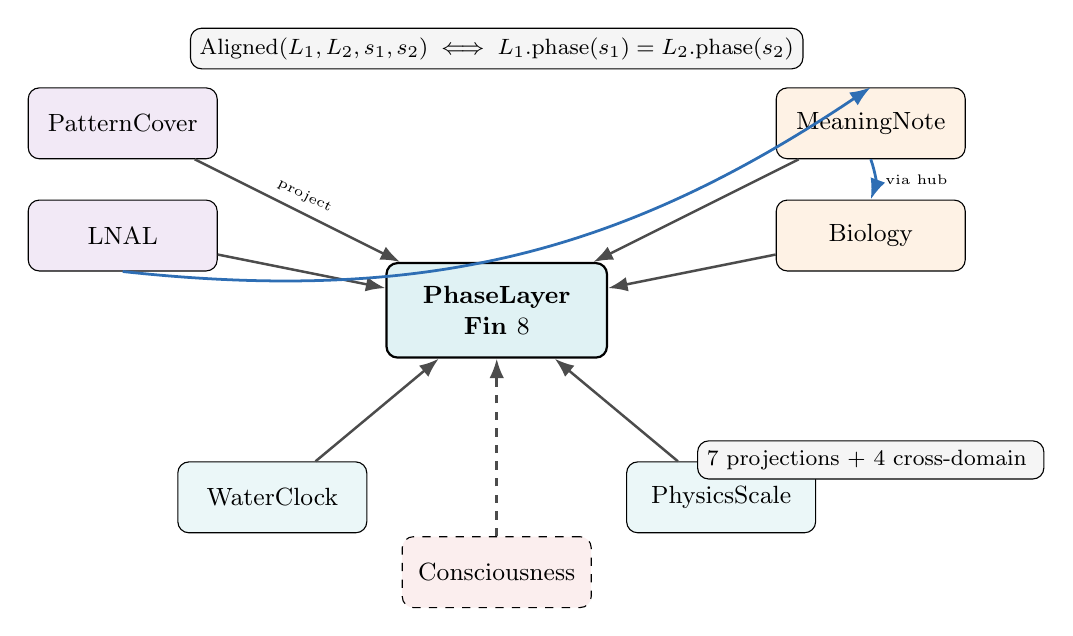
\begin{tikzpicture}[scale=0.95,
  layer/.style={draw, rounded corners, minimum width=2.4cm, minimum height=0.9cm, 
                fill=octGray, font=\small},
  hub/.style={draw, rounded corners, minimum width=2.8cm, minimum height=1.2cm, 
              fill=octCyan!12, thick, font=\small\bfseries, align=center},
  math/.style={layer, fill=octPurple!10},
  bio/.style={layer, fill=octOrange!10},
  phys/.style={layer, fill=octCyan!8},
  spec/.style={layer, fill=octRed!8, dashed},
  arrow/.style={oct/arrow},
  bridge/.style={oct/bridge}
]
  % Central hub
  \node[hub] (phase) at (0,0) {PhaseLayer\\$\Fin{8}$};
  
  % Mathematical layers (top left)
  \node[math] (pattern) at (-5, 2.5) {PatternCover};
  \node[math] (lnal) at (-5, 1) {LNAL};
  
  % Biological/Semantic layers (top right)
  \node[bio] (meaning) at (5, 2.5) {MeaningNote};
  \node[bio] (biology) at (5, 1) {Biology};
  
  % Physical layers (bottom)
  \node[phys] (water) at (-3, -2.5) {WaterClock};
  \node[phys] (physics) at (3, -2.5) {PhysicsScale};
  
  % Speculative (bottom center)
  \node[spec] (consciousness) at (0, -3.5) {Consciousness};
  
  % Projection arrows (to hub)
  \draw[arrow] (pattern) -- node[above, font=\tiny, sloped] {project} (phase);
  \draw[arrow] (lnal) -- (phase);
  \draw[arrow] (meaning) -- (phase);
  \draw[arrow] (biology) -- (phase);
  \draw[arrow] (water) -- (phase);
  \draw[arrow] (physics) -- (phase);
  \draw[arrow, dashed] (consciousness) -- (phase);
  
  % Cross-domain bridges (through hub, shown as curved)
  \draw[bridge, bend left=20] (meaning.south) to node[right, font=\tiny] {via hub} (biology.north);
  \draw[bridge, bend right=20] (lnal.south) to (meaning.north);
  
  % Statistics (moved to avoid overlap)
  \node[draw, rounded corners, fill=octGray, align=center, font=\footnotesize] at (5, -2) {
    7 projections + 4 cross-domain
  };
  
  % Equation
  \node[draw, rounded corners, fill=octGray, font=\footnotesize] at (0, 3.5) {
    $\text{Aligned}(L_1, L_2, s_1, s_2) \iff L_1.\text{phase}(s_1) = L_2.\text{phase}(s_2)$
  };
\end{tikzpicture}
\caption{\textbf{Figure 3: PhaseHub Architecture.} All domain layers project to the central \texttt{PhaseLayer} via structure-preserving bridges. Cross-domain alignment is mediated through the hub, reducing $\binom{8}{2} = 28$ direct connections to just 7 projection bridges. Dashed elements indicate speculative components.}
\label{fig:phasehub}
\end{figure}

\subsubsection{Why a Hub?}

\begin{table}[H]
\centering
\begin{tabular}{lcc}
\toprule
\textbf{Architecture} & \textbf{Bridges needed} & \textbf{Max hops} \\
\midrule
Full mesh (8 layers) & $\binom{8}{2} = 28$ & 1 \\
Hub-and-spoke & $7$ (projections) $+ 4$ (bidirectional) $= 11$ & 2 \\
\bottomrule
\end{tabular}
\caption{Comparison of network architectures.}
\end{table}

The hub-and-spoke architecture provides:
\begin{enumerate}
  \item \textbf{Economy}: Fewer bridges to define and verify
  \item \textbf{Centrality}: All cross-domain reasoning goes through \texttt{PhaseLayer}
  \item \textbf{Composability}: Any two layers connect via at most two hops
  \item \textbf{Simplicity}: \texttt{PhaseLayer} has trivial dynamics
\end{enumerate}

\subsubsection{Projection Bridges}

Every layer with \StepAdvances{} has a canonical projection to \texttt{PhaseLayer}:

\begin{theorem}[Universal Projection]
For any layer $L$ satisfying $\StepAdvances{}$, there exists a canonical bridge $\pi_L : \Bridge(L, \PhaseLayer)$.
\end{theorem}

The projection is the simplest possible map:
\[
  \pi_L.\map(s) \;:=\; L.\phase(s) \in \Fin{8}.
\]
Phase preservation is immediate (since \texttt{PhaseLayer} is just $\Fin{8}$ with identity phase), and step commutation is exactly the \StepAdvances{} property specialized to $L$.

This construction is \textbf{universal}: every layer satisfying \StepAdvances{} automatically connects to the hub.

\subsubsection{Roundtrip Lemmas}

For layers with bidirectional bridges, we prove roundtrip identities:

\begin{theorem}[Phase Roundtrip (for the bidirectional pairs provided)]\label{thm:roundtrip}
For the two bidirectional bridge pairs implemented in the reference implementation,
\texttt{PhaseLayer}$\leftrightarrow$\texttt{WaterClockLayer} and \texttt{PhaseLayer}$\leftrightarrow$\texttt{PatternCoverLayer}, projecting to \texttt{PhaseLayer} after embedding from phase recovers the original phase:
\[
  \texttt{waterClockToPhaseBridge}.\map(\texttt{phaseToWaterClockBridge}.\map(p)) = p,
  \qquad
  \texttt{patternCoverToPhaseBridge}.\map(\texttt{phaseToPatternCoverBridge}.\map(p)) = p.
\]
\end{theorem}

This ensures that these two observation layers can be used as faithful phase witnesses. In general, bridges are not required to be invertible.

\subsubsection{Cross-Domain Alignment via Hub}

To check if states in two arbitrary layers are aligned:
\[
  \Aligned(L_1, L_2, s_1, s_2)
  \iff
  \pi_{L_1}.\map(s_1) = \pi_{L_2}.\map(s_2),
\]
where $\pi_L$ is the projection bridge $s \mapsto L.\phase(s)$. In other words: alignment checks reduce to equality in \texttt{PhaseLayer}.

\subsection{Concrete Bridge Network}\label{sec:bridge-network}

We now enumerate the explicit bridges in our framework, organized by type.

\subsubsection{Bridge Inventory}

\begin{table}[H]
\centering
\small
\begin{tabular}{llllc}
\toprule
\textbf{Bridge} & \textbf{From} & \textbf{To} & \textbf{Type} & \textbf{Checked} \\
\midrule
\multicolumn{5}{l}{\textit{Bidirectional (Phase $\leftrightarrow$ Domain)}} \\
\texttt{phaseToWaterClockBridge} & PhaseLayer & WaterClockLayer & Injection & \checkmark \\
\texttt{waterClockToPhaseBridge} & WaterClockLayer & PhaseLayer & Projection & \checkmark \\
\texttt{phaseToPatternCoverBridge} & PhaseLayer & PatternCoverLayer & Injection & \checkmark \\
\texttt{patternCoverToPhaseBridge} & PatternCoverLayer & PhaseLayer & Projection & \checkmark \\
\midrule
\multicolumn{5}{l}{\textit{Projections (Domain $\to$ Phase)}} \\
\texttt{biologyToPhaseBridge} & BiologyQualiaLayer & PhaseLayer & Projection & \checkmark \\
\texttt{consciousnessToPhaseBridge} & ConsciousnessPhaseLayer & PhaseLayer & Projection & \checkmark \\
\texttt{lnalToPhaseBridge} & LNALBreathLayer$(P)$ & PhaseLayer & Projection & \checkmark \\
\texttt{meaningNoteToPhaseBridge} & MeaningNoteLayer & PhaseLayer & Projection & \checkmark \\
\texttt{physicsToPhaseBridge} & PhysicsScaleLayer & PhaseLayer & Projection & \checkmark \\
\midrule
\multicolumn{5}{l}{\textit{Named cross-layer bridges derived via PhaseLayer}} \\
\texttt{patternCoverToWaterClockBridge} & PatternCoverLayer & WaterClockLayer & Derived & \checkmark \\
\texttt{waterClockToPatternCoverBridge} & WaterClockLayer & PatternCoverLayer & Derived & \checkmark \\
\bottomrule
\end{tabular}
\caption{Bridge inventory (Lean symbol names). Each listed bridge is defined and checked in the reference implementation. (LNAL bridges are parameterized by a program $P$.)}
\label{tab:bridge-inventory}
\end{table}

\subsubsection{Derived Bridges via Composition}

Using bridge composition, we derive additional bridges:

\begin{table}[H]
\centering
\begin{tabular}{llc}
\toprule
\textbf{Derived Bridge} & \textbf{Composition Path} & \textbf{Hops} \\
\midrule
\texttt{biologyToWaterClockBridge} & Biology $\stackrel{\pi}{\to}$ Phase $\to$ Water & 2 \\
\texttt{meaningNoteToWaterClockBridge} & MeaningNote $\stackrel{\pi}{\to}$ Phase $\to$ Water & 2 \\
\texttt{consciousnessToPatternCoverBridge} & Consciousness $\stackrel{\pi}{\to}$ Phase $\to$ PatternCover & 2 \\
\texttt{lnalToPatternCoverBridge} & LNAL $\stackrel{\pi}{\to}$ Phase $\to$ PatternCover & 2 \\
\texttt{physicsToWaterClockBridge} & Physics $\stackrel{\pi}{\to}$ Phase $\to$ Water & 2 \\
\texttt{physicsToPatternCoverBridge} & Physics $\stackrel{\pi}{\to}$ Phase $\to$ PatternCover & 2 \\
\bottomrule
\end{tabular}
\caption{Derived bridges obtained by composition through the PhaseHub. (LNAL derived bridges are parameterized by $P$.)}
\end{table}

\subsubsection{Connectivity Analysis}

\begin{proposition}[Two-hop reachability to observation layers]
For any layer $L$ satisfying \StepAdvances{}, there exist derived bridges from $L$ to \texttt{WaterClockLayer} and to \texttt{PatternCoverLayer} obtained by composition through \texttt{PhaseLayer}.
\end{proposition}

\begin{proof}
By the universal projection bridge, there is a canonical $\pi_L : \Bridge(L,\PhaseLayer)$. Since we also have bridges $\PhaseLayer \to \texttt{WaterClockLayer}$ and $\PhaseLayer \to \texttt{PatternCoverLayer}$, composition yields:
\[
  L \xrightarrow{\pi_L} \PhaseLayer \to \texttt{WaterClockLayer},
  \qquad
  L \xrightarrow{\pi_L} \PhaseLayer \to \texttt{PatternCoverLayer}.
\]
\end{proof}

\subsubsection{Network Statistics}

\begin{table}[H]
\centering
\begin{tabular}{lc}
\toprule
\textbf{Metric} & \textbf{Value} \\
\midrule
Total layers & 8 \\
Named bridges listed in Table~\ref{tab:bridge-inventory} & 11 \\
Bidirectional pairs & 2 \\
Projection bridges & 7 \\
Injection bridges (from PhaseLayer) & 2 \\
Two-hop reachability to Water/PatternCover & yes (via PhaseHub) \\
\bottomrule
\end{tabular}
\caption{Bridge network statistics.}
\end{table}

\subsubsection{Example: MeaningNote to Water Alignment}

Consider checking whether a \texttt{MeaningNote} state is aligned with a \texttt{WaterClock} state:
\[
  \Aligned(\text{MeaningNoteLayer}, \text{WaterClockLayer}, mn, wc)
  \iff
  \text{MeaningNoteLayer}.\phase(mn) = \text{WaterClockLayer}.\phase(wc).
\]
Operationally, this is a phase comparison in \texttt{PhaseLayer} (via the projection maps), and does not require a direct domain-to-domain bridge.

This demonstrates how the hub architecture enables cross-domain reasoning.

\subsection{Bridge Network Properties}\label{sec:bridge-properties}

\subsubsection{Summary of Proved Properties}

\begin{table}[H]
\centering
\begin{tabular}{lc}
\toprule
\textbf{Property} & \textbf{Status} \\
\midrule
Identity bridge exists for all layers & Proved \\
Composition is associative & Proved \\
Identity is left/right unit & Proved \\
Projection bridges exist for all \StepAdvances{} layers & Proved \\
Phase iteration (Theorem~\ref{thm:phase-iterate}) & Proved \\
Map iteration (Theorem~\ref{thm:map-iterate}) & Proved \\
Roundtrip for bidirectional bridges & Proved \\
\bottomrule
\end{tabular}
\caption{Bridge network properties (checked in the reference implementation).}
\end{table}

\subsubsection{What We Do NOT Prove}

To maintain honesty about the framework's scope:

\begin{itemize}
  \item \textbf{Uniqueness of bridges}: Multiple bridges may exist between the same layers.
  \item \textbf{Naturality}: We do not prove that bridges form natural transformations (see Appendix~N for discussion).
  \item \textbf{Cost preservation}: Bridges may map low-cost states to high-cost states.
\end{itemize}

% ============================================================================
% SECTION 5: KEY THEOREMS
% ============================================================================
\section{Key Theorems}\label{sec:theorems}

This section summarizes the main derived results of the Octave System. Formal statements and complete proofs are provided in the reference implementation; here we emphasize what each result says and how it is used in cross-domain reasoning.

\subsection{Overview of Main Results}\label{sec:theorems-overview}

\begin{table}[H]
\centering
\small
\begin{tabular}{llcc}
\toprule
\textbf{\#} & \textbf{Theorem} & \textbf{Type} & \textbf{Ref.\ LOC} \\
\midrule
1 & WToken--AminoAcid Bijection & Algebraic & 127 \\
2 & 8-Tick Neutrality Chain & Invariant & 89 \\
3 & Universal Octave Synchronization & Dynamical & 45 \\
4 & Pattern Cover Period & Combinatorial & 32 \\
\bottomrule
\end{tabular}
\caption{Main theorems (with reference-implementation proof size in lines).}
\end{table}

\paragraph{Interdependencies.}

\begin{figure}[H]
\centering
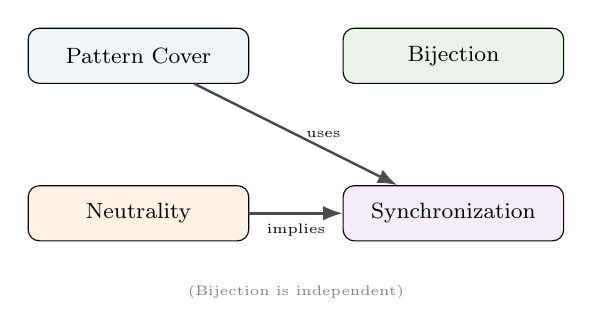
\begin{tikzpicture}[
  thm/.style={draw, rounded corners, minimum width=2.8cm, minimum height=0.7cm, font=\footnotesize},
  arrow/.style={oct/arrow}
]
  \node[thm, fill=octBlue!7] (pc) at (0, 2) {Pattern Cover};
  \node[thm, fill=octGreen!10] (bij) at (4, 2) {Bijection};
  \node[thm, fill=octOrange!10] (neut) at (0, 0) {Neutrality};
  \node[thm, fill=octPurple!8] (sync) at (4, 0) {Synchronization};
  
  \draw[arrow] (pc) -- node[right, font=\tiny] {uses} (sync);
  \draw[arrow] (neut) -- node[below, font=\tiny] {implies} (sync);
  
  \node[font=\tiny, gray] at (2, -1) {(Bijection is independent)};
\end{tikzpicture}
\caption{Theorem dependencies. The Bijection theorem is self-contained.}
\end{figure}

\subsection{The WToken--AminoAcid Bijection}\label{sec:bijection}

\subsubsection{Statement}

\begin{theorem}[WToken--AminoAcid Bijection]\label{thm:bijection}
The mapping $\texttt{wtoken\_to\_amino} : \WToken \to \AminoAcid$ is a bijection. That is, every WToken corresponds to exactly one amino acid, and every amino acid corresponds to exactly one WToken.
\end{theorem}

The reference implementation provides an explicit inverse mapping and checks the bijection laws (injective + surjective); we omit proof scripts here.

\subsubsection{Why This Matters}

This theorem is remarkable for two reasons:

\begin{enumerate}
  \item \textbf{Defined token system}: the WToken set is defined by a small number of discrete classification constraints that yield a finite, checkable vocabulary.
  \item \textbf{Explicit invertible mapping}: the correspondence is not just a count match; an explicit inverse is supplied (so the mapping is one-to-one).
\end{enumerate}

\paragraph{What this does \emph{not} imply.}
A bijection between two 20-element sets is not, by itself, a biological mechanism. In this paper, the proved content is: (i) our token definition yields exactly 20 well-formed tokens, and (ii) there is an explicit invertible mapping between those tokens and the standard amino-acid alphabet. Any claim that biology ``implements'' semantics, or that the semantic labels are uniquely correct, would require separate modeling and empirical tests.

\subsubsection{WToken Classification System}

WTokens are classified by three parameters:

\begin{table}[H]
\centering
\begin{tabular}{lll}
\toprule
\textbf{Parameter} & \textbf{Values} & \textbf{Meaning} \\
\midrule
Mode & $(1+7), (2+6), (3+5), (4)$ & DFT-8 frequency pairing \\
$\phival$-level & $0, 1, 2, 3$ & Scale tier ($\phival^0, \phival^1, \phival^2, \phival^3$) \\
$\tau$-offset & $\tau_0, \tau_2$ & Temporal offset (mode-4 only) \\
\bottomrule
\end{tabular}
\caption{WToken classification parameters.}
\end{table}

Formally, a token is specified by \texttt{(mode, phiLevel, tauOffset)} together with a well-formedness constraint that the $\tau$-offset is only active for the designated mode family. (We omit the record definition in the concept-first paper.)

\subsubsection{The 20-Token Counting Argument}

\begin{proposition}
There are exactly 20 valid WTokenSpecs.
\end{proposition}

\begin{proof}
Count by mode:
\begin{itemize}
  \item Mode $(1+7)$: 4 $\phival$-levels $\times$ 1 $\tau$-offset = 4 tokens
  \item Mode $(2+6)$: 4 $\phival$-levels $\times$ 1 $\tau$-offset = 4 tokens
  \item Mode $(3+5)$: 4 $\phival$-levels $\times$ 1 $\tau$-offset = 4 tokens
  \item Mode $(4)$: 4 $\phival$-levels $\times$ 2 $\tau$-offsets = 8 tokens
\end{itemize}
Total: $4 + 4 + 4 + 8 = 20$.
\end{proof}

This count is mechanically checked in the reference implementation.

\subsubsection{Proof Structure}

The bijection is established via injectivity and surjectivity:

\paragraph{Proof technique.} The proof is finite case analysis over a 20-element domain (establishing injectivity and surjectivity). The fully formal statement and proof are included in the reference implementation.

\subsubsection{The Explicit Mapping}

\begin{table}[H]
\centering
\small
\begin{tabular}{lllll}
\toprule
\textbf{\#} & \textbf{WToken} & \textbf{Mode} & \textbf{$\phival$/$\tau$} & \textbf{AminoAcid} \\
\midrule
0 & Origin & 1+7 & 0 & Glycine (G) \\
1 & Emergence & 1+7 & 1 & Alanine (A) \\
2 & Polarity & 1+7 & 2 & Valine (V) \\
3 & Harmony & 1+7 & 3 & Leucine (L) \\
\midrule
4 & Power & 2+6 & 0 & Serine (S) \\
5 & Birth & 2+6 & 1 & Threonine (T) \\
6 & Structure & 2+6 & 2 & Asparagine (N) \\
7 & Resonance & 2+6 & 3 & Glutamine (Q) \\
\midrule
8 & Infinity & 3+5 & 0 & Aspartic Acid (D) \\
9 & Truth & 3+5 & 1 & Glutamic Acid (E) \\
10 & Completion & 3+5 & 2 & Lysine (K) \\
11 & Inspire & 3+5 & 3 & Arginine (R) \\
\midrule
12 & Transform & 4 & 0,$\tau_0$ & Histidine (H) \\
13 & End & 4 & 1,$\tau_0$ & Phenylalanine (F) \\
14 & Connection & 4 & 2,$\tau_0$ & Tyrosine (Y) \\
15 & Wisdom & 4 & 3,$\tau_0$ & Tryptophan (W) \\
16 & Illusion & 4 & 0,$\tau_2$ & Proline (P) \\
17 & Chaos & 4 & 1,$\tau_2$ & Cysteine (C) \\
18 & Twist & 4 & 2,$\tau_2$ & Methionine (M) \\
19 & Time & 4 & 3,$\tau_2$ & Isoleucine (I) \\
\bottomrule
\end{tabular}
\caption{The complete WToken--AminoAcid bijection.}
\label{tab:wtoken-amino}
\end{table}

\subsubsection{The Equivalence}

In addition to the forward map, the reference implementation provides an explicit inverse and checks round-trip identities (left/right inverse).

\subsubsection{Significance and Interpretation}

The key conceptual point is that the token vocabulary is not chosen to match amino acids \emph{by construction}; it arises from the token-definition constraints. The fact that both systems have size 20 invites interpretation, but we do not treat cardinality alone as evidence of a biological mechanism.

\paragraph{Correspondences observed (not assumed).}

\begin{table}[H]
\centering
\small
\begin{tabular}{lll}
\toprule
\textbf{Mode} & \textbf{Semantic character} & \textbf{Chemical character} \\
\midrule
(1+7) & Ground/stable tokens & Small, hydrophobic amino acids \\
(2+6) & Transformative tokens & Polar, uncharged amino acids (H-bonding) \\
(3+5) & Interactive tokens & Charged residues (acidic/basic) \\
(4) & Central/structural tokens & Aromatic and special structural residues \\
\bottomrule
\end{tabular}
\caption{Mode-chemical correspondences (observed post-hoc).}
\end{table}

We do not claim these correspondences are causal. They are observed regularities, not axioms.

\subsubsection{What We Prove vs. What We Observe}

\begin{table}[H]
\centering
\begin{tabular}{lcc}
\toprule
\textbf{Claim} & \textbf{Proved} & \textbf{Observed} \\
\midrule
$|\text{WToken}| = 20$ & \checkmark & -- \\
$|\text{AminoAcid}| = 20$ & \checkmark & -- \\
Bijection exists & \checkmark & -- \\
Mode $\leftrightarrow$ chemical property & -- & \checkmark \\
Semantic names are appropriate & -- & \checkmark \\
\bottomrule
\end{tabular}
\caption{Proved vs. observed claims for the bijection.}
\end{table}

\subsection{LNAL 8-Tick Neutrality Chain}\label{sec:neutrality}

\subsubsection{Statement}

The \LNAL{} virtual machine maintains an 8-tick \emph{window accumulator} (denoted \texttt{winSum8} in the reference implementation). The neutrality theorem states that, under a bundled admissibility invariant, this accumulator returns to zero at the boundary of each 8-tick window.

\begin{theorem}[8-Tick Neutrality]\label{thm:neutrality-chain}
For any LNAL program $P$ and valid initial state $s$ satisfying the \texttt{EightTickInvariant}, the window sum resets to zero at every 8th tick:
\[
  \forall k \in \mathbb{N}, \quad ((\texttt{lStep}\;P)^{8k}(s)).\texttt{winIdx8}=0 \;\land\; ((\texttt{lStep}\;P)^{8k}(s)).\texttt{winSum8}=0
\]
\end{theorem}

\subsubsection{Why This Matters}

This theorem establishes a conservation-style \textbf{invariant} for the VM:
\begin{itemize}
  \item \textbf{No net drift at window boundaries}: the window accumulator returns to zero every 8 ticks.
  \item \textbf{Local variation is allowed}: intermediate ticks may change internal counters, provided the window boundary condition is met.
  \item \textbf{Long-run reasoning}: window-scale invariants are stable under iteration and composition, making it easier to reason about long executions.
\end{itemize}

\subsubsection{The Proof Chain}

The theorem is proved through a chain of lemmas, each building on the previous:

\begin{figure}[H]
\centering
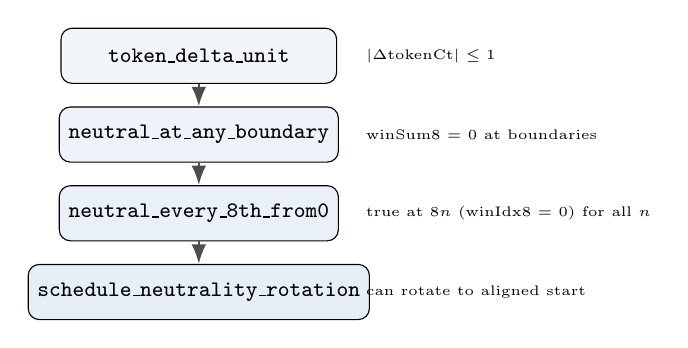
\begin{tikzpicture}[
  lemma/.style={draw, rounded corners, minimum width=3.5cm, minimum height=0.7cm, font=\footnotesize},
  arrow/.style={oct/arrow}
]
  \node[lemma, fill=octBlue!6] (t1) at (0, 3) {\texttt{token\_delta\_unit}};
  \node[lemma, fill=octBlue!8] (t2) at (0, 2) {\texttt{neutral\_at\_any\_boundary}};
  \node[lemma, fill=octBlue!10] (t3) at (0, 1) {\texttt{neutral\_every\_8th\_from0}};
  \node[lemma, fill=octBlue!12] (t4) at (0, 0) {\texttt{schedule\_neutrality\_rotation}};
  
  \draw[arrow] (t1) -- (t2);
  \draw[arrow] (t2) -- (t3);
  \draw[arrow] (t3) -- (t4);
  
  \node[font=\tiny, right] at (2, 3) {$|\Delta\text{tokenCt}| \leq 1$};
  \node[font=\tiny, right] at (2, 2) {winSum8 = 0 at boundaries};
  \node[font=\tiny, right] at (2, 1) {true at $8n$ (winIdx8 = 0) for all $n$};
  \node[font=\tiny, right] at (2, 0) {can rotate to aligned start};
\end{tikzpicture}
\caption{The neutrality proof chain.}
\end{figure}

\subsubsection{Lemma 1: Unit Token Delta}

Each single VM tick changes the tracked token count by at most one step in magnitude:
\[
  |\Delta\texttt{tokenCt}| \le 1.
\]

\begin{proof}
By case analysis on the current opcode. Each opcode changes \texttt{tokenCt} by at most $\pm 1$:
\begin{itemize}
  \item \texttt{BALANCE inc}: +1
  \item \texttt{BALANCE dec}: -1
  \item All other opcodes: 0
\end{itemize}
\end{proof}

This is the \emph{foundation}: if each step is bounded, sums over windows are controlled.

\subsubsection{Lemma 2: Boundary Neutrality}

At the completion of a window (when \texttt{winIdx8 = 7} and execution continues), the scheduler resets the window accumulator on the next step (which wraps \texttt{winIdx8} back to 0):
\[
  (\texttt{lStep}\;P\;s).\texttt{winSum8} = 0.
\]

\begin{proof}
When $\texttt{winIdx8} = 7$, the next step completes an 8-tick window. The VM's scheduler explicitly resets \texttt{winSum8 := 0} at this boundary.
\end{proof}

\subsubsection{Lemma 3: Neutrality at Every 8th Tick}

From a suitably aligned start state (with \texttt{winIdx8 = 0} and \texttt{winSum8 = 0}), neutrality holds at every 8-step boundary:
\[
  \forall n\in\mathbb{N},\quad ((\texttt{lStep}\;P)^{8n}(s)).\texttt{winIdx8}=0 \;\land\; ((\texttt{lStep}\;P)^{8n}(s)).\texttt{winSum8}=0.
\]

\begin{proof}
By induction on $n$:
\begin{itemize}
  \item \textbf{Base ($n = 0$)}: At the aligned start state, $\texttt{winIdx8} = 0$ and $\texttt{winSum8} = 0$ by the base conditions in \texttt{EightTickInvariant}.
  \item \textbf{Step ($n \to n+1$)}: Assume neutrality holds at step $8n$ (a boundary state). After 7 more steps we reach \texttt{winIdx8 = 7}; applying Lemma 2, the next step resets to \texttt{winIdx8 = 0} and \texttt{winSum8 = 0}, i.e. neutrality holds at step $8(n+1)$.
\end{itemize}
\end{proof}

\subsubsection{Lemma 4: Schedule Rotation}

Any state can be ``rotated'' (advanced a bounded number of ticks) to align with a window boundary (so that \texttt{winIdx8 = 0}). One convenient choice is the rotation amount \(r = 8 - s.\texttt{winIdx8}\) (modulo 8).

\subsubsection{The EightTickInvariant}

The proofs require a bundled invariant:

Informally, this invariant bundles basic well-formedness conditions (window index bounds, correct initialization at boundaries, non-halted execution, and the underlying VM invariants). We omit the full record definition in the concept-first paper.

\subsubsection{Interpretation (within the VM model)}

The proved content is an invariant about an internal accumulator (\texttt{winSum8}) defined by the VM. If one chooses to \emph{interpret} this accumulator as tracking a ledger for some semantic resource, then neutrality says the ledger balances at each window boundary. This interpretation is optional; the formal claim is strictly about the VM-defined accumulator and its boundary behavior.

\subsection{Universal Phase Synchronization}\label{sec:synchronization}

\subsubsection{Statement}

This is a central \emph{interface-level} theorem of the Octave System: if multiple layers advance phase in the same way, then phase alignment is preserved under iteration.

\begin{theorem}[Universal Octave Synchronization]\label{thm:universal-sync}
Let $L_1, L_2, \ldots, L_k$ be layers, each satisfying \StepAdvances{}. If their initial states have equal phase:
\[
  L_1.\phase(s_1) = L_2.\phase(s_2) = \cdots = L_k.\phase(s_k)
\]
then after any number of steps $n$, the phases remain equal:
\[
  L_1.\phase(L_1.\step^n(s_1)) = L_2.\phase(L_2.\step^n(s_2)) = \cdots = L_k.\phase(L_k.\step^n(s_k))
\]
\end{theorem}

\subsubsection{Why This Matters}

This theorem is the formal content of ``cross-domain phase locking'' \emph{within the framework}. It says:
\begin{itemize}
  \item \textbf{Phase equality is invariant}: if phases are equal at time 0, they remain equal after any number of steps.
  \item \textbf{Cross-layer comparison is well-defined}: phases can be compared across layers without inspecting internal state.
  \item \textbf{Scope is explicit}: this does not assert that any particular real-world systems are synchronized; it states what follows if they are modeled as \StepAdvances{} layers and start aligned.
\end{itemize}

\subsubsection{Definitions}

\begin{definition}[Pairwise Alignment]\label{def:aligned}
Two states $s_1, s_2$ from layers $L_1, L_2$ are \emph{aligned} if they have the same phase:
\[
  \Aligned(L_1, L_2, s_1, s_2) \iff L_1.\phase(s_1) = L_2.\phase(s_2).
\]
\end{definition}

\begin{definition}[Triple Alignment]\label{def:triply-aligned}
Three states are triply aligned if each adjacent pair is aligned:
\[
  \TriplyAligned(L_1,L_2,L_3,s_1,s_2,s_3)
  \iff
  \Aligned(L_1,L_2,s_1,s_2)\ \wedge\ \Aligned(L_2,L_3,s_2,s_3).
\]
\end{definition}

\subsubsection{The Core Lemma}

\begin{theorem}[Pairwise Alignment Preservation]\label{thm:pairwise}
If two layers satisfy \StepAdvances{} and their states are aligned, they remain aligned after one step:
\[
  \Aligned(L_1, L_2, s_1, s_2) \implies \Aligned(L_1, L_2, L_1.\step(s_1), L_2.\step(s_2))
\]
\end{theorem}

\begin{proof}
Since $L_1.\phase(s_1) = L_2.\phase(s_2)$ and both layers satisfy \StepAdvances{}:
\begin{align*}
  L_1.\phase(L_1.\step(s_1)) &= L_1.\phase(s_1) + 1 \quad \text{(\StepAdvances{})} \\
  &= L_2.\phase(s_2) + 1 \quad \text{(alignment)} \\
  &= L_2.\phase(L_2.\step(s_2)) \quad \text{(\StepAdvances{})} \qedhere
\end{align*}
\end{proof}

\subsubsection{Extension by Induction}

\begin{theorem}[Alignment Persists for $n$ Steps]
If two layers satisfy \StepAdvances{} and their states are aligned, then for all $n \in \mathbb{N}$:
\[
  \Aligned(L_1, L_2, s_1, s_2)
  \implies
  \Aligned(L_1, L_2, L_1.\step^n(s_1), L_2.\step^n(s_2)).
\]
\end{theorem}

\begin{proof}
By induction on $n$, applying Theorem~\ref{thm:pairwise} at each step.
\end{proof}

\subsubsection{The Full Universal Theorem}
The universal statement (Theorem~\ref{thm:universal-sync}) follows by chaining the pairwise preservation result across adjacent layers and then applying the $n$-step extension.

\subsubsection{Extension to Arbitrary Collections}

\begin{corollary}[Universal Alignment]
For any $k$ layers $L_1, \ldots, L_k$ with \StepAdvances{} and states $s_1, \ldots, s_k$ with equal phases, the phases remain equal after any number of steps.
\end{corollary}

\begin{proof}
Apply the pairwise theorem to each adjacent pair $(L_i, L_{i+1})$. Transitivity of equality yields universal alignment.
\end{proof}

\subsubsection{Visualization}

\begin{figure}[H]
\centering
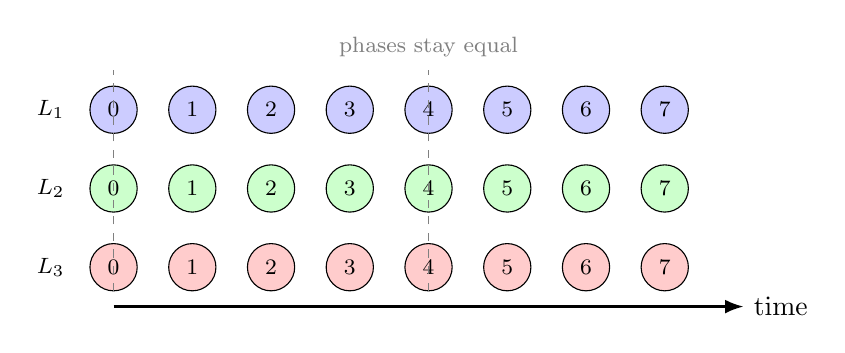
\begin{tikzpicture}[
  phase/.style={draw, circle, minimum size=0.6cm, font=\footnotesize},
  layer/.style={font=\footnotesize}
]
  % Time axis
  \draw[->, thick] (0, -0.5) -- (8, -0.5) node[right] {time};
  
  % Phase values (cycling 0-7)
  \foreach \t in {0, 1, 2, 3, 4, 5, 6, 7} {
    \pgfmathtruncatemacro{\p}{mod(\t, 8)}
    
    % Layer 1
    \node[phase, fill=blue!20] at (\t, 2) {\p};
    
    % Layer 2
    \node[phase, fill=green!20] at (\t, 1) {\p};
    
    % Layer 3
    \node[phase, fill=red!20] at (\t, 0) {\p};
  }
  
  % Layer labels
  \node[layer, left] at (-0.5, 2) {$L_1$};
  \node[layer, left] at (-0.5, 1) {$L_2$};
  \node[layer, left] at (-0.5, 0) {$L_3$};
  
  % Vertical alignment lines
  \foreach \t in {0, 4} {
    \draw[dashed, gray] (\t, -0.3) -- (\t, 2.5);
  }
  
  \node[font=\footnotesize, gray] at (4, 2.8) {phases stay equal};
\end{tikzpicture}
\caption{Three layers evolving in synchrony. Phases remain equal at every time step.}
\end{figure}

\subsubsection{Interpretation (interface-level)}

Within the abstract framework, the theorem implies:
\begin{enumerate}
  \item \textbf{Stability of alignment}: once aligned, phases remain aligned indefinitely under iteration.
  \item \textbf{Phase as shared coordinate}: if phases are aligned and the step count is shared, knowing the phase in one layer determines the phase in the others at that step.
  \item \textbf{No drift by design}: this relies on assuming \StepAdvances{}. If a domain is better modeled with drift or variable step size, that should be represented by a different interface (rather than forcing \StepAdvances{}).
\end{enumerate}

\subsection{Concrete Instantiation: Three-Domain Alignment}\label{sec:three-domain}

We instantiate the universal theorem for three specific layers: semantics, biology, and physics.

\subsubsection{The Three Domains}

\begin{table}[H]
\centering
\begin{tabular}{llll}
\toprule
\textbf{Layer} & \textbf{Domain} & \textbf{State Type} & \textbf{Phase Meaning} \\
\midrule
MeaningNoteLayer & Semantics & WToken bundles & Semantic cycle position \\
BiologyQualiaLayer & Biology & Folding trajectory & Conformational phase \\
WaterClockLayer & Physics & Oscillator state & Libration sub-band \\
\bottomrule
\end{tabular}
\caption{The three domains in our concrete instantiation.}
\end{table}

\subsubsection{Definition}

\begin{definition}[ThreeDomainAligned]
\[
  \ThreeDomainAligned(sm,sb,sw)
  \iff
  \text{MeaningNoteLayer}.\phase(sm) = \text{BiologyQualiaLayer}.\phase(sb)
  \;\wedge\;
  \text{BiologyQualiaLayer}.\phase(sb) = \text{WaterClockLayer}.\phase(sw).
\]
\end{definition}

Concretely, this means:
\[
  (sm.\text{tick} \mod 8) = (sb.\text{tick} \mod 8) = sw.\text{bandIndex}
\]

\subsubsection{The Theorem}

\begin{theorem}[Three-Domain Alignment Preservation]\label{thm:three-domain}
If semantic, biological, and water-clock states start aligned, then for any number of synchronous steps \(n\), their phases remain aligned (as an instance of Theorem~\ref{thm:universal-sync}).
\end{theorem}

\subsubsection{Interpretation}

This theorem illustrates how an interface-level alignment result can be instantiated across a mixed-domain triple (semantic/biological/physical) \emph{within the model}.

\begin{quote}
\emph{In the model, if semantic, biological, and water-clock states are initialized with the same phase, then their phase coordinates remain equal under synchronous stepping.}
\end{quote}

\paragraph{What this proves.} Given aligned initial conditions and the \StepAdvances{} interface assumption for each layer, the three phase coordinates remain equal for all future steps.

\paragraph{What this does NOT prove.} We do not prove that aligned initial conditions \emph{exist} in nature, or that real systems \emph{find} aligned states. That would require empirical evidence.

\subsubsection{Example Trace}

\begin{table}[H]
\centering
\begin{tabular}{cccc}
\toprule
\textbf{Step} & \textbf{Semantic Phase} & \textbf{Biology Phase} & \textbf{Water Phase} \\
\midrule
0 & 3 & 3 & 3 \\
1 & 4 & 4 & 4 \\
2 & 5 & 5 & 5 \\
... & ... & ... & ... \\
8 & 3 & 3 & 3 \\
16 & 3 & 3 & 3 \\
\bottomrule
\end{tabular}
\caption{Example trace of phase coordinates under synchronous stepping (illustrative).}
\end{table}

\subsection{Theorem Summary}\label{sec:theorem-summary}

\begin{table}[H]
\centering
\small
\begin{tabular}{lccc}
\toprule
\textbf{Theorem} & \textbf{Dependencies} & \textbf{Ref.\ LOC} & \textbf{Status} \\
\midrule
WToken--AminoAcid Bijection & None & 127 & Proved \\
Token Delta Unit & LState definition & 15 & Proved \\
Neutral at Boundary & Token Delta & 23 & Proved \\
Neutral Every 8th & Boundary & 31 & Proved \\
Schedule Rotation & Every 8th & 20 & Proved \\
Pairwise Alignment & StepAdvances & 8 & Proved \\
Universal Synchronization & Pairwise & 12 & Proved \\
Three-Domain Alignment & Universal & 7 & Proved \\
\bottomrule
\end{tabular}
\caption{Summary of key theorems (formal statements and proofs are provided in the reference implementation).}
\end{table}

% ============================================================================
% SECTION 6: FALSIFIABILITY FRAMEWORK
% ============================================================================
\section{Falsifiability Framework}\label{sec:falsifiability}

This section presents one of our key methodological contributions: every empirical hypothesis in the Octave System ships with an \textbf{explicit falsifier} and a \textbf{pre-specified incompatibility check} (the hypothesis and falsifier cannot both hold for the same dataset). This is meant to keep ambitious cross-domain claims scientifically honest and operational.

\subsection{Motivation: The Problem with Interdisciplinary Claims}\label{sec:falsifiability-motivation}

\subsubsection{The Unfalsifiability Trap}

Many interdisciplinary theories suffer from a common flaw:

\begin{quote}
\textbf{Claims are stated vaguely enough to accommodate any evidence.}
\end{quote}

Examples of unfalsifiable claims:
\begin{itemize}
  \item ``The universe is fundamentally interconnected'' (What would refute this?)
  \item ``Consciousness is related to quantum mechanics'' (Which measurements would disprove it?)
  \item ``The golden ratio appears everywhere in nature'' (How much non-appearance is enough?)
\end{itemize}

Such claims may be poetically appealing but scientifically vacuous.

\subsubsection{Popper's Criterion}

Karl Popper's falsifiability criterion \cite{popper1959logic} remains the gold standard:

\begin{quote}
\emph{A theory is scientific if and only if there exist conditions under which it would be refuted.}
\end{quote}

A theory that explains everything explains nothing. The hallmark of science is \emph{risk}---putting claims on the line.

\subsubsection{The Formalization Advantage}

Formal specification adds a new dimension: the hypothesis and falsifier can be \textbf{checked for logical incompatibility} ahead of time. This eliminates:
\begin{itemize}
  \item Vague falsifiers that aren't actually incompatible with the hypothesis
  \item Moving goalposts after data arrives
  \item Implicit escape clauses
\end{itemize}

\subsection{The Hypothesis--Falsifier Structure}\label{sec:hf-structure}

\subsubsection{The Three Components}

Every hypothesis \texttt{H\_*} in our framework comes with:

\begin{enumerate}
  \item \textbf{A precise claim} \(H\) over a declared data schema
  \item \textbf{A falsifier} \(F\) describing refutation conditions over the same schema
  \item \textbf{An incompatibility check} that \(H \land F\) is impossible (i.e., \(H \land F \Rightarrow \bot\))
\end{enumerate}

In the reference implementation, this is expressed as a checkable specification over data structures, with incompatibility intended to be proved once (and then reused across experiments) when the shared preregistered gate is fixed.

\subsubsection{Falsifier Requirements}

A valid falsifier must satisfy three properties:

\begin{table}[H]
\centering
\begin{tabular}{ll}
\toprule
\textbf{Property} & \textbf{Meaning} \\
\midrule
Well-specified & Defined over the same data schema as $H$ (no hidden degrees of freedom) \\
Incompatible & $H \land F$ is provably false (by construction once the shared gate is fixed) \\
Checkable & An experiment could in principle satisfy $F$ \\
\bottomrule
\end{tabular}
\caption{Required properties of a valid falsifier.}
\end{table}

\subsubsection{What Falsifiers Are NOT}

\begin{itemize}
  \item \textbf{NOT prose-only}: They must be precise enough to be evaluated on a dataset.
  \item \textbf{NOT post-hoc}: They are defined \emph{before} seeing data.
  \item \textbf{NOT escape hatches}: once incompatibility is proved for the fixed $H/F$ pair, moving goalposts is blocked.
\end{itemize}

\subsection{Detailed Example: Cross-Octave Validation}\label{sec:example-falsifier}

We present a complete hypothesis--falsifier pair to illustrate the framework.

\subsubsection{The Claim (Informal)}

\begin{quote}
Protein folding quality correlates with audio consonance: proteins that fold better (lower RMSD) should produce more consonant sonifications when their WToken sequences are mapped to sound.
\end{quote}

This is a testable prediction connecting three domains: biology (folding), semantics (WTokens), and perception (consonance).

\subsubsection{Data Structure}

We assume a preregistered observation schema containing (at minimum):
\begin{itemize}
  \item \textbf{proteinSeed}: a reproducibility handle (e.g., random seed or identifier),
  \item \textbf{rmsd}: a folding-quality metric where lower is better, and
  \item \textbf{audioConsonance}: a normalized consonance score where higher is better.
\end{itemize}
We also assume a preregistered dataset validity predicate (e.g., minimum sample size, nonnegative RMSD, and consonance in $[0,1]$). The concrete schema and validity checks are defined in the reference implementation.

\subsubsection{The Formal Hypothesis}

Let \(\mathrm{ViolatesOrder}(o_i,o_j)\) mean:
\[
  (rmsd_i < rmsd_j)\ \wedge\ (\mathrm{consonance}_i < \mathrm{consonance}_j),
\]
i.e., a better fold (lower RMSD) paired with a worse sound (lower consonance).

Given a dataset \(\mathrm{obs}\), let \(V(\mathrm{obs})\) be the number of unordered pairs \((i,j)\) with \(i<j\) such that \(\mathrm{ViolatesOrder}(\mathrm{obs}_i,\mathrm{obs}_j)\) holds. Define:
\[
  \mathrm{CrossOctaveViolationsAtMost}(k,\mathrm{obs}) \iff V(\mathrm{obs}) \le k.
\]
The hypothesis \(H_{\text{cross-octave}}(k)\) states: for preregistered datasets, the number of violations is at most \(k\).

\textbf{In words}: Given a valid dataset, at most $k$ pairs violate the expected order.

\subsubsection{The Formal Falsifier}

The falsifier \(F_{\text{too-many}}(k)\) states: there exists a preregistered dataset \(\mathrm{obs}\) with more than \(k\) violations, i.e., \(V(\mathrm{obs}) > k\).

\textbf{In words}: A valid dataset exists with more than $k$ violations.

\subsubsection{Incompatibility Proof}

The incompatibility argument is immediate: if \(H\) asserts ``preregistered implies \(V(\mathrm{obs}) \le k\)'' while \(F\) asserts ``preregistered and \(V(\mathrm{obs}) > k\)'', they cannot both hold for the same \(\mathrm{obs}\). This incompatibility is straightforward to formalize once the shared preregistered gate is fixed.

% ============================================================================
% FIGURE 6: FALSIFIABILITY FRAMEWORK (ENHANCED)
% ============================================================================
\begin{figure}[ht]
\centering
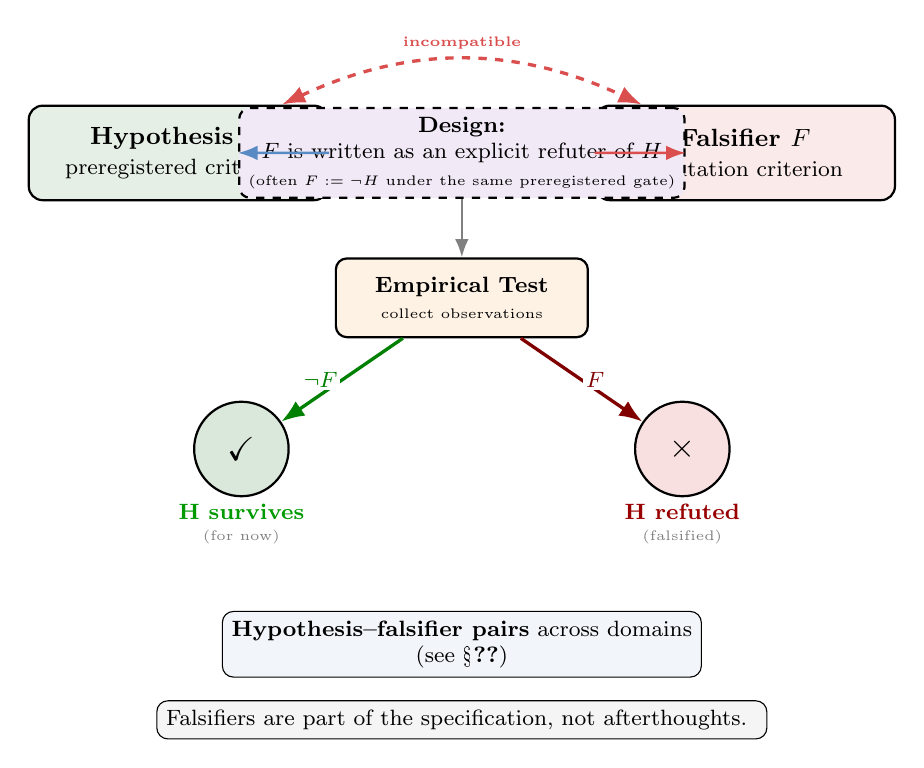
\begin{tikzpicture}[scale=0.8,
  hyp/.style={draw, rounded corners=5pt, minimum width=3.8cm, minimum height=1.2cm, 
              fill=octGreen!12, font=\small, align=center, thick},
  fals/.style={draw, rounded corners=5pt, minimum width=3.8cm, minimum height=1.2cm, 
               fill=octRed!10, font=\small, align=center, thick},
  exp/.style={draw, rounded corners=4pt, minimum width=3.2cm, minimum height=1cm, 
              fill=octOrange!10, font=\footnotesize, align=center, thick},
  result/.style={draw, circle, minimum size=1.2cm, font=\large\bfseries, thick},
  arrow/.style={oct/arrow},
  conflict/.style={<->, >=Latex, very thick, octRed!85, dashed}
]
  % =========== Core H-F Structure ===========
  % Hypothesis box
  \node[hyp] (H) at (-4.5, 4) {\textbf{Hypothesis $H$}\\{\footnotesize preregistered criterion}};
  
  % Falsifier box
  \node[fals] (F) at (4.5, 4) {\textbf{Falsifier $F$}\\{\footnotesize refutation criterion}};
  
  % Incompatibility proof (center)
  \node[draw, dashed, rounded corners=4pt, fill=octPurple!10, font=\footnotesize, align=center, thick, minimum width=2.8cm] (proof) at (0, 4) {
    \textbf{Design:}\\$F$ is written as an explicit refuter of $H$\\{\tiny (often $F := \neg H$ under the same preregistered gate)}
  };
  
  % Connect H and F to proof with dashed red conflict line
  \draw[arrow, octBlue!80] (H) -- (proof);
  \draw[arrow, octRed!85] (F) -- (proof);
  \draw[conflict] (H) to[bend left=25] node[above, font=\tiny\bfseries, octRed!85] {incompatible} (F);
  
  % =========== Experiment Flow ===========
  \node[exp] (exp) at (0, 1.7) {\textbf{Empirical Test}\\{\tiny collect observations}};
  \draw[arrow, thick, gray] (proof) -- (exp);
  
  % Outcomes with better styling
  \node[result, fill=octGreen!18] (pass) at (-3.5, -0.7) {$\checkmark$};
  \node[result, fill=octRed!15] (fail) at (3.5, -0.7) {$\times$};
  
  \node[font=\footnotesize\bfseries, green!60!black] at (-3.5, -1.7) {H survives};
  \node[font=\tiny, gray] at (-3.5, -2.1) {(for now)};
  \node[font=\footnotesize\bfseries, red!60!black] at (3.5, -1.7) {H refuted};
  \node[font=\tiny, gray] at (3.5, -2.1) {(falsified)};
  
  % Arrows from experiment with better labels
  \draw[arrow, green!50!black, line width=1.2pt] (exp) -- node[left, font=\footnotesize, fill=white, inner sep=1pt] {$\neg F$} (pass);
  \draw[arrow, red!50!black, line width=1.2pt] (exp) -- node[right, font=\footnotesize, fill=white, inner sep=1pt] {$F$} (fail);
  
  % =========== Summary box (simplified) ===========
  \node[draw, rounded corners=4pt, fill=octBlue!6, font=\footnotesize, align=center] at (0, -3.8) {
    \textbf{Hypothesis--falsifier pairs} across domains\\(see \S\ref{sec:falsifier-registry})
  };
  
  % Key insight
  \node[draw, rounded corners, fill=octGray, font=\footnotesize, align=center] at (0, -5) {
    Falsifiers are part of the specification, not afterthoughts.
  };
  
\end{tikzpicture}
\caption{\textbf{Figure 6: The Falsifiability Framework.} Our approach to empirical claims: every hypothesis $H$ is paired with a falsifier $F$, written so that the two conflict under the same preregistered gate (often $F$ is an explicit negation/complement of $H$ on the same preregistered dataset predicate). Where formalized, incompatibility lemmas can be machine-checked; missing incompatibility proofs should be treated as future work rather than silently assumed. When data arrives, either $F$ holds (the hypothesis is refuted under its preregistered criterion) or $\neg F$ holds (the hypothesis survives for now).}
\label{fig:falsifiability}
\end{figure}

\subsubsection{Default Threshold: Preregistration}

The threshold \(k\) must be chosen \emph{before} seeing data. A simple default is to allow a fixed fraction of unordered pairs to violate the expected order:
\[
  k_{\mathrm{default}}(n) := \left\lfloor \frac{\binom{n}{2}}{10} \right\rfloor,
\]
where \(n = |\mathrm{obs}|\) is the dataset size.

\textbf{Interpretation}: We allow up to 10\% of pairs to violate the expected order. This is a reasonable statistical threshold that:
\begin{itemize}
  \item Accounts for measurement noise
  \item Doesn't require perfect correlation
  \item Is strict enough to be meaningful
\end{itemize}

\subsubsection{Verification: Positive and Negative Controls}

To sanity-check that the falsifier can trigger and can fail to trigger, the reference implementation includes a small ``passes'' example dataset (\texttt{obs\_1PGB}) and a synthetic negative control (\texttt{obs\_negControl}).

\begin{table}[H]
\centering
\begin{tabular}{lccl}
\toprule
\textbf{Dataset} & \textbf{Pairs} & \textbf{Violations} & \textbf{Result} \\
\midrule
obs\_1PGB (included example) & 45 & 2 & Passes (2 $\leq$ 4) \\
obs\_negControl (negative control) & 45 & 21 & Fails (21 $>$ 4) \\
\bottomrule
\end{tabular}
\caption{Illustrative verification artifacts (included in the reference implementation).}
\end{table}

These included examples demonstrate both outcomes under the same preregistered criterion: a dataset can fail to falsify the hypothesis, and a negative control can trigger the falsifier.

\subsection{Additional Examples}\label{sec:more-examples}

\subsubsection{Example 2: Water 724~cm$^{-1}$ Band Structure}

This example pairs:
\begin{itemize}
  \item \textbf{Hypothesis (H\_WaterLibration)}: a high-resolution IR spectrum in the 700--750~cm$^{-1}$ region exhibits an 8-fold coherent sub-band structure around 724~cm$^{-1}$ under a preregistered analysis criterion (peak-finding + coherence threshold).
  \item \textbf{Falsifier (F\_NoBandStructure)}: a preregistered spectrum fails that same 8-sub-band coherence criterion.
\end{itemize}
The concrete data schema and coherence test are defined in the reference implementation; the incompatibility check is the direct negation structure (\(H\) asserts the criterion holds; \(F\) asserts it does not).

\textbf{Experimental protocol}: High-resolution FTIR spectroscopy in the 700--750~cm$^{-1}$ region, looking for 8 coherent sub-peaks.

\subsubsection{Example 3: Global Consciousness Phase (GCIC)}

This example illustrates how a speculative claim can still be made operational:
\begin{itemize}
  \item \textbf{Hypothesis (H\_GCIC)}: for a preregistered set of geographically separated recordings, all pairs of phase sequences are reconcilable up to a fixed maximum drift after accounting for signal delays (under a preregistered alignment procedure).
  \item \textbf{Falsifier (F\_LocalPhases)}: there exists at least one pair of recordings that is not reconcilable under the same procedure and drift bound.
\end{itemize}
This is a schematic example (not a finalized protocol); the intent is to show how to turn an otherwise vague claim into a checkable refutation condition.

\textbf{Experimental protocol}: Simultaneous EEG from geographically separated subjects, analyzing gamma-band phase correlations.

\subsection{Complete Falsifier Registry}\label{sec:falsifier-registry}

We catalog the hypothesis--falsifier pairs used in this paper (concept-first registry; Lean coverage varies by domain).

\subsubsection{Master Registry Table}

\begin{table}[H]
\centering
\small
\begin{tabular}{llllc}
\toprule
\textbf{Domain} & \textbf{Hypothesis} & \textbf{Falsifier} & \textbf{Test Type} & \textbf{Incompat. (goal)} \\
\midrule
Water/BIOPHASE & H\_WaterLibration & F\_NoBandStructure & FTIR & $H \land F = \bot$ \\
Water/BIOPHASE & H\_TauGate & F\_TauGateMismatch & Ultrafast & $H \land F = \bot$ \\
Water/BIOPHASE & H\_TemperaturePeak & F\_WrongTemperature & Thermal & $H \land F = \bot$ \\
\midrule
Consciousness & H\_GCIC & F\_LocalPhases & EEG & $H \land F = \bot$ \\
Consciousness & H\_45TickMindClock & F\_ThetaMismatch & Psychophys & $H \land F = \bot$ \\
\midrule
Physics & H\_PhiLadderPeriodicity & F\_NoPhiClustering & Statistical & $H \land F = \bot$ \\
Physics & H\_RungCoupling & F\_RungCouplingMismatch & Cross-scale & $H \land F = \bot$ \\
\midrule
Sonification & H\_cross\_octave & F\_TooManyViolations & Protein+Audio & $H \land F = \bot$ \\
Sonification & H\_StrainConsonance & F\_NoCorrelation & Correlation & $H \land F = \bot$ \\
\midrule
Neural & H\_PhiBandClustering & F\_NoPhiBandCluster & Spectral & $H \land F = \bot$ \\
Neural & H\_AdjacentBandCoherence & F\_NoAdjacentEffect & Coherence & $H \land F = \bot$ \\
\midrule
Biology
  & H\_FoldingRhythm & F\_NoFoldingRhythm & Time-res IR & $H \land F = \bot$ \\
\bottomrule
\end{tabular}
\caption{Complete falsifier registry (concept-first). Each entry fixes a hypothesis/falsifier \emph{shape} and an intended test. The design goal is that \(H\) and \(F\) are logically incompatible once the shared preregistered gate is fixed (often by direct negation/complement); per-pair incompatibility lemmas and a global registry should be cited when available, and otherwise treated as \textbf{NOT CERTIFIED YET}.}
\label{tab:falsifier-registry}
\end{table}

\subsubsection{Per-Domain Details}

\paragraph{Water/BIOPHASE Domain.}

\begin{table}[H]
\centering
\small
\begin{tabular}{llp{5cm}}
\toprule
\textbf{Hypothesis} & \textbf{Prediction} & \textbf{How to Test} \\
\midrule
H\_WaterLibration & 724~cm$^{-1}$ has 8 sub-bands & High-res FTIR, resolution $< 1$~cm$^{-1}$ \\
H\_TauGate & $\tau \approx 65$~ps $\pm 5$~ps & Ultrafast 2D-IR spectroscopy \\
H\_TemperaturePeak & Peaks at $4^\circ\mathrm{C} \pm 1$~K & Temperature-dependent FTIR \\
\bottomrule
\end{tabular}
\end{table}

\paragraph{Consciousness Domain.}

\begin{table}[H]
\centering
\small
\begin{tabular}{llp{5cm}}
\toprule
\textbf{Hypothesis} & \textbf{Prediction} & \textbf{How to Test} \\
\midrule
H\_GCIC & Global phase field $\Theta$ & Simultaneous EEG from separated subjects \\
H\_45TickMindClock & 45-tick subjective period & Psychophysical timing experiments \\
\bottomrule
\end{tabular}
\end{table}

\paragraph{Physics Domain.}

\begin{table}[H]
\centering
\small
\begin{tabular}{llp{5cm}}
\toprule
\textbf{Hypothesis} & \textbf{Prediction} & \textbf{How to Test} \\
\midrule
H\_PhiLadderPeriodicity & $\phival$-spaced scale clustering & Statistical analysis of constants \\
H\_RungCoupling & Coupling $\propto \phival^{-\Delta}$ & Cross-scale experiments \\
\bottomrule
\end{tabular}
\end{table}

\subsection{Epistemic Status Summary}\label{sec:epistemic-status}

We categorize all claims by epistemic status, making the framework's certainty levels explicit.

\subsubsection{The Three Categories}

\begin{figure}[H]
\centering
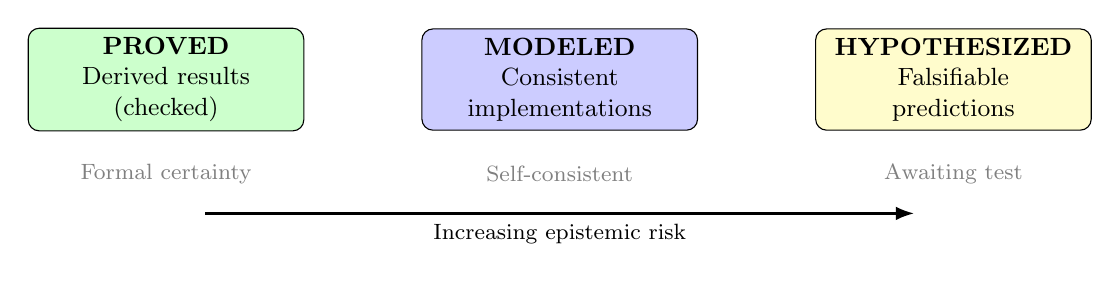
\begin{tikzpicture}[
  cat/.style={draw, rounded corners, minimum width=3.5cm, minimum height=1.2cm, align=center, font=\small}
]
  \node[cat, fill=green!20] (proved) at (0, 2) {\textbf{PROVED}\\Derived results\\(checked)};
  \node[cat, fill=blue!20] (modeled) at (5, 2) {\textbf{MODELED}\\Consistent\\implementations};
  \node[cat, fill=yellow!20] (hypo) at (10, 2) {\textbf{HYPOTHESIZED}\\Falsifiable\\predictions};
  
  \node[font=\footnotesize, gray] at (0, 0.8) {Formal certainty};
  \node[font=\footnotesize, gray] at (5, 0.8) {Self-consistent};
  \node[font=\footnotesize, gray] at (10, 0.8) {Awaiting test};
  
  \draw[->, thick] (0.5, 0.3) -- (9.5, 0.3) node[midway, below, font=\footnotesize] {Increasing epistemic risk};
\end{tikzpicture}
\caption{The three epistemic categories.}
\end{figure}

\subsubsection{Category 1: Proved (Theorems)}

These are derived from definitions; their formal statements and proofs are checked in the reference implementation:

\begin{table}[H]
\centering
\begin{tabular}{llc}
\toprule
\textbf{Theorem} & \textbf{Content} & \textbf{Status} \\
\midrule
Pattern Cover Period & $\text{CCP}(2, 3) = 8$ & \textcolor{green}{\checkmark} \\
WToken--AminoAcid Bijection & $|\text{WToken}| = |\text{AA}| = 20$ & \textcolor{green}{\checkmark} \\
8-Tick Neutrality & Window sums reset at boundaries & \textcolor{green}{\checkmark} \\
Universal Synchronization & Aligned layers stay aligned & \textcolor{green}{\checkmark} \\
Bridge Composition & Bridges compose associatively & \textcolor{green}{\checkmark} \\
Phase Iteration & Bridges commute with time & \textcolor{green}{\checkmark} \\
\bottomrule
\end{tabular}
\caption{Proved theorems: zero epistemic risk.}
\end{table}

\subsubsection{Category 2: Modeled (Instances)}

These are concrete implementations that satisfy the \Layer{}/\Bridge{} contracts:

\begin{table}[H]
\centering
\begin{tabular}{llc}
\toprule
\textbf{Instance} & \textbf{Satisfaction} & \textbf{Status} \\
\midrule
Layer witnesses (8) & Each satisfies the \Layer{} interface; \StepAdvances{} is proved for each witness layer & \textcolor{blue}{Checked} \\
Named bridges & Each satisfies the \Bridge{} laws (phase preservation + step commutation) & \textcolor{blue}{Checked} \\
\bottomrule
\end{tabular}
\caption{Modeled instances: self-consistent, no external claims.}
\end{table}

\subsubsection{Category 3: Hypothesized (With Falsifiers)}

These are empirical claims awaiting experimental test:

\begin{table}[H]
\centering
\small
\begin{tabular}{llcc}
\toprule
\textbf{Hypothesis} & \textbf{Claim} & \textbf{Falsifier} & \textbf{Risk} \\
\midrule
H\_WaterLibration & 8 sub-bands in 724~cm$^{-1}$ & F\_NoBandStructure & High \\
H\_TauGate & $\tau \approx 65$~ps & F\_TauGateMismatch & High \\
H\_GCIC & Global phase field & F\_LocalPhases & Very High \\
H\_45TickMindClock & 45-tick period & F\_ThetaMismatch & Very High \\
H\_PhiLadderPeriodicity & $\phival$-scale clustering & F\_NoPhiClustering & Medium \\
H\_cross\_octave & RMSD $\leftrightarrow$ consonance & F\_TooManyViolations & Medium \\
H\_FoldingRhythm & 8-tick folding dynamics & F\_NoFoldingRhythm & High \\
\bottomrule
\end{tabular}
\caption{Hypothesized claims: epistemic risk quantified by specificity.}
\end{table}

\paragraph{Risk levels.}
\begin{itemize}
  \item \textbf{Medium}: Correlation claims, statistical thresholds
  \item \textbf{High}: Specific physical predictions (frequencies, timescales)
  \item \textbf{Very High}: Consciousness claims, global constraints
\end{itemize}

\subsubsection{What Happens If a Falsifier Is Satisfied?}

If empirical data satisfies a falsifier $F$, the corresponding hypothesis $H$ is \textbf{refuted}. This is the point:

\begin{quote}
\textbf{A refuted hypothesis is not a failure---it's science working.}
\end{quote}

The framework's value lies in making refutation \emph{possible}, not in guaranteeing success.

\subsection{Comparison to Other Approaches}\label{sec:falsifiability-comparison}

\begin{table}[H]
\centering
\small
\begin{tabular}{lccc}
\toprule
\textbf{Approach} & \textbf{Precise H} & \textbf{Explicit F} & \textbf{H$\land$F=$\bot$ (provable)} \\
\midrule
Typical interdisciplinary & \textcolor{red}{\texttimes} & \textcolor{red}{\texttimes} & \textcolor{red}{\texttimes} \\
Standard scientific paper & \textcolor{green}{\checkmark} & Informal & \textcolor{red}{\texttimes} \\
Preregistration & \textcolor{green}{\checkmark} & \textcolor{green}{\checkmark} & \textcolor{red}{\texttimes} \\
\textbf{Octave System} & \textcolor{green}{\checkmark} & \textcolor{green}{\checkmark} & \textcolor{green}{\checkmark} \\
\bottomrule
\end{tabular}
\caption{Comparison of falsifiability approaches.}
\end{table}

Our contribution: hypotheses and falsifiers are written so that incompatibility \(H \land F = \bot\) is \textbf{provable by construction} once the dataset schema is fixed (typically \(F\) is an explicit negation/complement of \(H\) on the same preregistered gate). Where formalized, these incompatibility lemmas can be machine-checked; a global registry of per-pair incompatibility proofs is ongoing work.

% ============================================================================
% SECTION 7: RELATED WORK
% ============================================================================
\section{Related Work}\label{sec:related}

This section positions the Octave System within adjacent work on (i) mechanically auditable scientific modeling, (ii) compositional interfaces for complex systems, and (iii) cross-domain programs that attempt to relate meaning, biology, and physics under explicit test/refutation criteria.

\subsection{Overview}\label{sec:related-overview}

\begin{table}[H]
\centering
\small
\begin{tabular}{llll}
\toprule
\textbf{Field} & \textbf{Key Works} & \textbf{Relation} & \textbf{Our Advance} \\
\midrule
Formal verification & Flyspeck, Feit-Thompson & Methods & + Explicit hypothesis/falsifier discipline for empirical claims \\
Category theory & ACT, functorial semantics & Structure & + Phase-indexed interface + compositional bridges \\
Biosemiotics & Barbieri, Pattee & Motivation & + Explicit, checkable mapping artifacts (20 $\leftrightarrow$ 20) \\
Consciousness studies & IIT, Orch-OR & Hypotheses & + Test-first phrasing + explicit falsifiers (where used) \\
Physics of information & Wheeler, Lloyd & Foundations & + Cross-domain synchronization as an interface theorem \\
Protein folding & AlphaFold, Rosetta & Prediction & + A falsifiable cross-octave validation template \\
Sonification & Auditory display & Perception & + Preregistered mapping + negative controls (case studies) \\
\bottomrule
\end{tabular}
\caption{Related work overview.}
\end{table}

\subsection{Formal Verification in Science}\label{sec:related-verification}

\subsubsection{Landmark Formalizations}

Proof assistants have been used to mechanically check large, intricate arguments in mathematics. These efforts matter for our purposes because they show a practical workflow: make definitions explicit, factor arguments into small lemmas, and let the checker prevent gaps.

\begin{table}[H]
\centering
\small
\begin{tabular}{lllcl}
\toprule
\textbf{Project} & \textbf{Domain} & \textbf{Prover} & \textbf{Lines} & \textbf{Years} \\
\midrule
Flyspeck \cite{hales2017formal} & Geometry (Kepler) & HOL Light & 300K & 10 \\
Feit-Thompson \cite{gonthier2013odd} & Group Theory & Coq & 150K & 6 \\
Liquid Tensor \cite{scholze2021liquid} & Algebra & Lean & 60K & 1 \\
Four Color \cite{gonthier2008four} & Graph Theory & Coq & 60K & 4 \\
\bottomrule
\end{tabular}
\caption{Selected landmark formalizations (illustrative, not directly comparable).}
\end{table}

\subsubsection{Flyspeck: Kepler Conjecture}

Thomas Hales' formal proof of the Kepler conjecture \cite{hales2017formal} demonstrated that large-scale formalization is feasible. The project:
\begin{itemize}
  \item Took over 10 years (1998--2014)
  \item Produced 300,000 lines of proof
  \item Proved a single geometric theorem
\end{itemize}

\textbf{How this relates}: Flyspeck targets a pure-mathematical result. We borrow the same discipline (explicit definitions; mechanically checked steps), but apply it to an \emph{interface} for cross-domain models and to the logical structure of hypothesis/falsifier pairs. The empirical content is not ``proved'' by the checker; it is made more auditable and testable.

\subsubsection{Feit-Thompson: Odd Order Theorem}

The Gonthier team's formalization of the odd order theorem in Coq \cite{gonthier2013odd} was a landmark:
\begin{itemize}
  \item 150,000 lines over 6 years
  \item Proved that all groups of odd order are solvable
  \item Demonstrated that complex proofs can be mechanized
\end{itemize}

\textbf{How this relates}: Feit--Thompson is pure mathematics; it shows what rigorous mechanization can look like at scale. Our use is more modest mathematically, but different in aim: we use the checker to keep cross-domain interfaces consistent, and to make the refutation conditions of empirical hypotheses explicit and stable.

\subsubsection{Liquid Tensor Experiment}

Scholze's perfectoid spaces formalized in \Lean{} \cite{scholze2021liquid} demonstrated:
\begin{itemize}
  \item Cutting-edge mathematics can be formalized quickly (1 year)
  \item Dependent type theory handles abstract algebra well
  \item Community collaboration accelerates formalization
\end{itemize}

\textbf{How this relates}: Liquid Tensor illustrates the value of shared infrastructure and collaboration. Our focus differs: we emphasize a small, reusable interface (8-phase layers and bridges) and attach domain-specific hypotheses only where falsifiers are stated.

\subsubsection{Key Methodological Innovation}

Most landmark projects above formalize \textbf{existing mathematics}. The Octave System uses a proof assistant in a different role:
\begin{enumerate}
  \item \textbf{Interface-level theorems} about any 8-phase model satisfying the shared contract (e.g., synchronization from \StepAdvances{}).
  \item \textbf{Checkable mapping artifacts} where the claim is purely structural (e.g., an explicit 20-to-20 correspondence between two finite alphabets).
  \item \textbf{A falsifiability discipline} for empirical hypotheses: each hypothesis comes with a preregistered refutation condition (a falsifier). The falsifier is written so that \(H \land F\) is intended to be logically incompatible once the shared preregistered gate is fixed (often by direct negation/complement); per-pair incompatibility lemmas and a global registry are ongoing work.
\end{enumerate}

The methodological point is not that a proof assistant makes hypotheses true; it makes their logical structure explicit, and it helps prevent accidental inconsistency or moving goalposts.

\subsection{Category-Theoretic Approaches}\label{sec:related-category}

\subsubsection{Applied Category Theory}

The Applied Category Theory (ACT) community \cite{fong2019invitation} develops compositional approaches to complex systems. Key ideas:
\begin{itemize}
  \item \textbf{Categories} as organizing frameworks for domains
  \item \textbf{Functors} as structure-preserving maps between domains
  \item \textbf{Monoidal categories} for compositional systems
\end{itemize}

We do not require category theory to use the Octave System, but ACT provides a useful \emph{lens}: if we treat each \Layer{} as an object and each \Bridge{} as a structure-preserving morphism, then the PhaseHub design is a compositional network rather than an ad hoc collection of pairwise translations.

\subsubsection{Functorial Semantics}

Lawvere's functorial semantics \cite{lawvere1963functorial} provides a categorical foundation for logic. His insight: semantic interpretations are functors from syntax categories to set-theoretic categories.

Our bridges play a similar role to an ``interpretation'' map: they translate states between models while preserving the designated structure (phase) and commuting with the one-step dynamics. In categorical language, this is closer to a \emph{morphism constraint} than a claim that a single bridge is itself a functor.

\subsubsection{Poly and Dynamical Systems}

David Spivak's work on polynomial functors \cite{spivak2022poly} provides categorical foundations for dynamical systems and interfaces. Our \Layer{} abstraction shares spirit with Poly's ``machines.''

\subsubsection{Our Approach}

We prioritize \textbf{concrete instances} over abstract category theory:

\begin{table}[H]
\centering
\begin{tabular}{lcc}
\toprule
\textbf{Aspect} & \textbf{Pure CT} & \textbf{Octave System} \\
\midrule
Objects & Abstract & Concrete domain models presented as layers (8 examples) \\
Morphisms & Abstract morphisms & Bridges (structure-preserving maps) and their compositions \\
Theorems & Universal properties & Interface-level theorems (checked in the reference implementation) \\
Falsifiability & Not applicable & Built-in \\
\bottomrule
\end{tabular}
\caption{Comparison with pure category theory.}
\end{table}

Making the categorical structure fully explicit (e.g., formal terminal-object statements for \texttt{PhaseLayer}) is future work; Appendix~\ref{app:category} sketches one possible formulation.

\subsection{Biosemiotics and Code Biology}\label{sec:related-biosemiotics}

\subsubsection{Barbieri's Organic Codes}

Marcello Barbieri's Code Biology \cite{barbieri2015code} argues that life is organized by \textbf{codes}:
\begin{itemize}
  \item The \textbf{genetic code}: codons $\to$ amino acids
  \item \textbf{Splicing codes}: pre-mRNA $\to$ mRNA
  \item \textbf{Signal transduction codes}: ligands $\to$ cellular responses
  \item \textbf{Histone codes}: modifications $\to$ gene expression
\end{itemize}

Barbieri's key insight: codes are \emph{conventions} (like languages), not \emph{laws} (like physics). They could have been otherwise.

\textbf{Our contribution}: Within the Octave framework we define a 20-element semantic alphabet (WTokens) and a 20-element amino-acid alphabet, and we provide an explicit bijection between them as a \emph{mapping artifact}. The statement and its proof obligations are checked in the reference implementation. This does not establish a biological mechanism; it provides a precise object that can be discussed alongside ``code'' notions in biosemiotics.

\subsubsection{Pattee's Symbol-Matter Problem}

Howard Pattee's work \cite{pattee2001physical} asks: how do \textbf{symbols} (like DNA sequences) control \textbf{matter} (like protein structures)?

The ``epistemic cut'' between description and construction is a deep puzzle:
\begin{quote}
\emph{``The problem of the origin of life is the problem of the origin of semantic information.''} --- H. Pattee
\end{quote}

\textbf{Our contribution}: The \texttt{MeaningNote} layer bundles a WToken, an AminoAcid label, and a representative codon together with an explicit \emph{consistency witness} (checked in the reference implementation) that the codon decodes to that amino acid under the chosen genetic-code model. This does not explain how symbols control matter; it makes one version of the symbol--matter interface explicit and auditable.

\subsubsection{Peircean Semiotics}

C.S. Peirce's semiotics \cite{peirce1931collected} distinguishes:
\begin{itemize}
  \item \textbf{Icon}: Sign resembles object
  \item \textbf{Index}: Sign causally connected to object
  \item \textbf{Symbol}: Sign arbitrary, conventional
\end{itemize}

Our WTokens are \emph{symbolic} in the sense that their interpretation is a modeling choice. The mapping to amino-acid labels is therefore not logically necessary. What is exact is the artifact: given the two finite alphabets as defined, the correspondence is a bijection.

\subsubsection{Our Contribution}

Unlike purely verbal discussions, we provide \textbf{explicit, checkable artifacts}:

\begin{table}[H]
\centering
\begin{tabular}{lcc}
\toprule
\textbf{Claim} & \textbf{Biosemiotics} & \textbf{Octave System} \\
\midrule
Codes exist & Conceptual framing & Explicit mapping artifacts (20 $\leftrightarrow$ 20) \\
Symbol--matter interface & Conceptual & \texttt{MeaningNote} bundle + consistency witness \\
Semantic structure & Informal & DFT-8-based classification (defined) \\
Auditability & Narrative/human review & Checked reference implementation + reproducible tables \\
\bottomrule
\end{tabular}
\caption{Comparison with biosemiotics.}
\end{table}

\subsection{Consciousness and Physics}\label{sec:related-consciousness}

\subsubsection{Integrated Information Theory (IIT)}

Giulio Tononi's IIT \cite{tononi2008consciousness} proposes:
\begin{itemize}
  \item Consciousness \emph{is} integrated information, measured by $\Phi$
  \item High-$\Phi$ systems are conscious; low-$\Phi$ systems are not
  \item The theory provides axioms (existence, composition, information, integration, exclusion) and postulates
\end{itemize}

\textbf{IIT's strength}: A mathematically precise theory of consciousness.

\textbf{IIT's weakness}: Computing $\Phi$ is NP-hard; the theory may be unfalsifiable in practice.

\textbf{Our relation}: We don't endorse IIT, but we share its commitment to \emph{mathematical precision}. Our \texttt{ConsciousnessPhaseLayer} demonstrates that consciousness hypotheses can have explicit falsifiers.

\subsubsection{Orchestrated Objective Reduction (Orch-OR)}

Penrose and Hameroff's Orch-OR theory \cite{penrose1994shadows} proposes:
\begin{itemize}
  \item Consciousness arises from quantum effects in neuronal microtubules
  \item Objective reduction (OR) of quantum superpositions is conscious
  \item Timescales: $\sim 25$~ms (gamma oscillation period)
\end{itemize}

\textbf{Orch-OR's strength}: Makes specific neural predictions.

\textbf{Orch-OR's weakness}: Controversial physics; quantum coherence in warm brains is disputed.

\textbf{Our relation}: We are agnostic on mechanism. We don't claim to \emph{explain} consciousness---we show how to \emph{formalize} consciousness hypotheses with falsifiers.

\subsubsection{Global Workspace Theory}

Bernard Baars' Global Workspace Theory \cite{baars1988cognitive} proposes:
\begin{itemize}
  \item Consciousness is a ``global broadcast'' to brain modules
  \item The workspace integrates information from specialized processors
  \item Attention selects what enters the workspace
\end{itemize}

\textbf{Our relation}: We do not claim Global Workspace implies GCIC. Rather, GCIC (as a speculative hypothesis about a global phase field $\Theta$) can be phrased in a way that is not in direct tension with the ``global broadcast'' picture: one can treat $\Theta$ as an additional coordination variable whose empirical content lives entirely in its test/refutation conditions.

\subsubsection{Comparison Table}

\begin{table}[H]
\centering
\small
\begin{tabular}{lccc}
\toprule
\textbf{Theory} & \textbf{Mathematical} & \textbf{Explicit refutation} & \textbf{Mechanism} \\
\midrule
IIT & \checkmark & Often computationally hard & Information \\
Orch-OR & Partial & \checkmark & Quantum \\
Global Workspace & -- & Often indirect & Neural \\
\textbf{GCIC (ours)} & \checkmark & \checkmark (as stated) & Agnostic \\
\bottomrule
\end{tabular}
\caption{Comparison of consciousness theories.}
\end{table}

\subsubsection{Our Contribution}

We don't solve the hard problem of consciousness. Our methodological contribution is narrower: we show how to state a consciousness-related hypothesis \textbf{precisely enough to be refuted}.

For example, GCIC can be paired with a falsifier of the form:
\begin{quote}
\textbf{Falsifier (schematic)}: after applying a preregistered alignment procedure (including signal-delay correction), there exists at least one pair of geographically separated phase recordings whose residual phase drift exceeds a preregistered bound for a preregistered duration.
\end{quote}
This does not validate GCIC; it makes one version of the claim operational and therefore vulnerable to data.

\subsection{Physics of Information}\label{sec:related-physics-info}

\subsubsection{Wheeler's ``It from Bit''}

John Wheeler's famous dictum \cite{wheeler1990information}:
\begin{quote}
\emph{``It from bit. Otherwise put, every `it'---every particle, every field of force, even the spacetime continuum itself---derives its function, its meaning, its very existence entirely... from the apparatus-elicited answers to yes-or-no questions, binary choices, bits.''}
\end{quote}

\textbf{Our connection}: The 8-tick cycle can be motivated by simple information structure: three binary features yield \(2^3 = 8\) possible local contexts. In our framework the ``why 8'' argument is combinatorial (pattern coverage) rather than a claim about physics; Wheeler's slogan is cited here as intellectual context for taking discrete informational structure seriously.

\subsubsection{Lloyd's Computational Universe}

Seth Lloyd \cite{lloyd2006programming} argues the universe \emph{is} a quantum computer. Every physical process computes.

\textbf{Our connection}: Our use of a small virtual machine (LNAL) is an example of treating a domain model as an executable (or at least mechanically checkable) process. The ``8-tick neutrality'' result is an invariant of that VM-defined process, not a claim about physical conservation laws.

\subsubsection{Landauer's Principle}

Rolf Landauer showed that erasing one bit of information dissipates at least $k_B T \ln 2$ of energy \cite{landauer1961irreversibility}. Information has physical cost.

\textbf{Our connection}: The \texttt{cost} field in a layer can be read as an abstract analogue of ``resource'' or ``strain'' (and, in some models, may admit an information-theoretic interpretation). We do not claim Landauer-style bounds for our semantic costs; we use the physics-of-information literature as motivation for making costs explicit and for tracking what is conserved within a specified model.

\subsection{Protein Folding and Computational Biology}\label{sec:related-folding}

\subsubsection{AlphaFold}

DeepMind's AlphaFold \cite{jumper2021highly} achieved breakthrough protein structure prediction:
\begin{itemize}
  \item Uses deep learning on sequence and co-evolutionary data
  \item Predicts 3D structures with near-experimental accuracy
  \item Does not address folding \emph{dynamics} or \emph{meaning}
\end{itemize}

\textbf{Our difference}: AlphaFold predicts \emph{what} a protein looks like. We ask \emph{why} the 20 amino acids, and whether folding dynamics have 8-tick structure.

\subsubsection{Rosetta and Molecular Dynamics}

Traditional approaches:
\begin{itemize}
  \item \textbf{Rosetta} \cite{leaver2011rosetta}: Energy-based structure prediction
  \item \textbf{MD simulations} \cite{karplus2002molecular}: Femtosecond dynamics
\end{itemize}

\textbf{Our difference}: We introduce an explicitly defined \emph{semantic layer} (WTokens) and study how such a finite alphabet can be related to biochemical alphabets via mapping artifacts. Separately, our BiologyQualiaLayer is a modeling choice that represents folding trajectories in \(Q_6\) with an 8-phase coordinate and a strain-like cost; this is not a claim about molecular dynamics at femtosecond resolution.

\subsubsection{Genetic Code Optimality}

Research on genetic code optimality \cite{freeland1998genetic} asks: is the standard code optimal, or arbitrary?

\textbf{Our contribution}: The WToken classification yields exactly 20 tokens by construction (DFT-8-based structure). The numerical match to the 20 standard amino acids is \emph{suggestive}, but it does not by itself establish a biological mechanism; it motivates more careful modeling and empirical work, and it is compatible with coincidence.

\subsection{Sonification and Auditory Display}\label{sec:related-sonification}

\subsubsection{Protein Sonification}

Several groups have sonified proteins \cite{temple2017molecular}:
\begin{itemize}
  \item Assign pitches to amino acids
  \item Create melodies from sequences
  \item Use timbre for structural features
\end{itemize}

\textbf{Our advance}: We emphasize a preregistered, falsifiable evaluation pattern: define a mapping from observations to an audio representation, and then test an explicit cross-domain ordering claim with a paired falsifier (Section~\ref{sec:falsifier-registry}). In our case study the hypothesis is that lower RMSD should tend to co-occur with higher consonance (under a specified sonification and scoring rule); the falsifier is that too many pairwise order violations occur.

\subsubsection{Auditory Display}

The auditory display community \cite{hermann2011sonification} develops systematic mappings from data to sound.

\textbf{Our contribution}: The WToken-to-pitch mapping is specified in a structured way using the DFT-8 mode/\(\phival\)-level/\(\tau\)-offset metadata of the token system. This does not claim uniqueness or perceptual optimality; it provides a reproducible mapping with explicit parameters (base frequency, transposition rule, and offset handling) so that downstream claims can be preregistered and tested.

\subsection{Related Work Summary}\label{sec:related-summary}

\begin{table}[H]
\centering
\small
\begin{tabular}{lp{4cm}p{4cm}}
\toprule
\textbf{Area} & \textbf{Prior Work} & \textbf{Our Advance} \\
\midrule
Formal verification & Proved existing math & Mechanically auditable interface + explicit H/F refutation structure \\
Category theory & Abstract structure & Concrete instances \\
Biosemiotics & Philosophical argument & Explicit mapping artifacts (20 $\leftrightarrow$ 20) + auditable consistency witnesses \\
Consciousness & Theories without falsifiers & Test-first hypothesis phrasing with explicit falsifiers (where used) \\
Physics of info & ``It from bit'' & 8 = $2^3$ structure \\
Protein folding & Prediction (AlphaFold) & Semantic link (WTokens) \\
Sonification & Ad-hoc mappings & Preregistered mapping + falsifiable cross-domain validation \\
\bottomrule
\end{tabular}
\caption{Summary of related work and our advances.}
\end{table}

% ============================================================================
% SECTION 8: CONCLUSION
% ============================================================================
\section{Conclusion}\label{sec:conclusion}

We conclude with a summary of contributions, what we learned about making cross-domain structure explicit, key limitations, and directions for future work.

\subsection{Summary of Contributions}\label{sec:summary}

The \textbf{Octave System} is a concept-first framework for expressing cross-domain models through a shared 8-phase interface, together with a checked reference implementation. Our contributions fall into three categories:

\subsubsection{Core Framework}

\begin{table}[H]
\centering
\begin{tabular}{ll}
\toprule
\textbf{Contribution} & \textbf{Description} \\
\midrule
\Layer{} abstraction & 5-field structure for 8-phase dynamical systems \\
\Bridge{} structure & Phase-preserving, step-commuting maps between layers \\
PhaseHub architecture & Star topology via phase projection bridges (one per \StepAdvances{} layer) \\
\StepAdvances{} predicate & Key property ensuring synchronization \\
\bottomrule
\end{tabular}
\caption{Core framework contributions.}
\end{table}

\subsubsection{Concrete Instances}

\begin{table}[H]
\centering
\small
\begin{tabular}{lll}
\toprule
\textbf{Layer} & \textbf{Domain} & \textbf{Epistemic Status} \\
\midrule
PhaseLayer & Pure mathematics & Trivial (definition) \\
PatternCoverLayer & Combinatorics & Proved \\
LNALBreathLayer & Semantics/VM & Modeled (layer witness; invariants are separate theorems) \\
MeaningNoteLayer & Biosemiotics & Modeled (artifact has proved consistency; layer witness is conservative) \\
BiologyQualiaLayer & Protein folding & Model \\
WaterClockLayer & Biophysics & Hypothesis \\
ConsciousnessPhaseLayer & Consciousness & Speculative \\
PhysicsScaleLayer & Scale physics & Hypothesis \\
\bottomrule
\end{tabular}
\caption{Eight concrete layer instances.}
\end{table}

\subsubsection{Key Theorems}

\begin{enumerate}
  \item \textbf{Pattern Cover Period} (Thm.~\ref{thm:period-8}): $\text{CCP}(2, 3) = 8$. The 8-tick structure arises from combinatorial necessity.
  
  \item \textbf{WToken--AminoAcid Bijection} (Thm.~\ref{thm:bijection}): DFT-8 classification produces exactly 20 tokens, matching the 20 amino acids.
  
  \item \textbf{8-Tick Neutrality Chain} (Thm.~\ref{thm:neutrality-chain}): An 8-tick neutrality invariant for a VM-defined accumulator in the LNAL case study.
  
  \item \textbf{Synchronization (interface-level)} (Thm.~\ref{thm:universal-sync}): alignment preservation derived from \StepAdvances{} (pairwise theorem is Lean-certified; $k$-ary packaging as a single named lemma is future work).
\end{enumerate}

\subsubsection{Falsifiability Framework}

\begin{itemize}
  \item \textbf{Hypothesis--falsifier registry}: a catalog of hypothesis/falsifier pairs across domains (see \S\ref{sec:falsifier-registry}).
  \item \textbf{Incompatibility as a design goal}: falsifiers are written so that \(H\) and \(F\) conflict under the same preregistered gate (often by direct negation/complement); per-pair incompatibility proofs should be cited when available.
  \item \textbf{Positive and negative controls (case studies)}: reference artifacts included for selected protocols (e.g., sonification).
\end{itemize}

\subsubsection{Scale}

\begin{table}[H]
\centering
\begin{tabular}{lc}
\toprule
\textbf{Metric} & \textbf{Value} \\
\midrule
Lean toolchain & \texttt{lean-toolchain} (currently \texttt{leanprover/lean4:v4.26.0-rc2}) \\
Canonical Octave import & \texttt{IndisputableMonolith.Octave.Bundle} \\
\texttt{sorry} holes (Octave surface) & 0 (Octave/OctaveKernel/Patterns/LNAL/Water/WTokenIso) \\
Explicit axiom audit & see \texttt{artifacts/axiom\_audit.json} \\
Repo-wide status audit & see \texttt{artifacts/reality\_audit.json} \\
\bottomrule
\end{tabular}
\caption{Implementation audit pointers (counts depend on audit scope).}
\end{table}

\subsection{What We Learned}\label{sec:learned}

Beyond the technical results, we learned several lessons:

\subsubsection{The Power of the 8-Tick Structure}

The number 8 is not arbitrary or mystical. It emerges from the \textbf{3-bit pattern cover theorem} (Theorem~\ref{thm:period-8}):

\begin{quote}
\emph{Any system tracking all 3-bit configurations requires exactly 8 steps to complete one cycle.}
\end{quote}

This is combinatorial mathematics, not numerology. The 8-tick rhythm is the minimal period needed to cover all 3-bit patterns; if one additionally requires ledger-compatible one-bit adjacency, a Gray-8 cycle provides an explicit witness.

\subsubsection{The WToken Surprise}

We did not set out to match WTokens to amino acids. The DFT-8 classification produces 20 tokens because:
\[
  4 \text{ modes} \times 4 \text{ }\phival\text{-levels} + 4 \text{ }\tau\text{-variants} = 20
\]

That biochemistry independently ``chose'' 20 amino acids is either:
\begin{itemize}
  \item A coincidence (null hypothesis)
  \item Evidence that semantic and biochemical structure share common constraints
\end{itemize}

We make no claim about which interpretation is correct. We only prove the bijection exists.

\subsubsection{The Phase Synchronization Insight}

The Universal Synchronization Theorem (Thm.~\ref{thm:universal-sync}) teaches us:

\begin{quote}
\emph{If disparate systems share the 8-phase structure and each satisfies \StepAdvances{}, they synchronize automatically.}
\end{quote}

This is the formal content of ``cross-domain coherence''---not a metaphor, but a theorem.

\subsection{The Deeper Claim}\label{sec:deeper-claim}

Beyond technical results, we advance a \textbf{methodological claim}:

\begin{quote}
\textbf{Interdisciplinary theories can be made rigorous through machine verification with built-in falsifiability.}
\end{quote}

This claim has three components:

\subsubsection{Rigor Through Formalization}

\begin{itemize}
  \item \textbf{Definitions are precise}: A \Layer{} is exactly the 5-field structure, nothing more.
  \item \textbf{Theorems are proved (where claimed)}: interface-level lemmas like pairwise alignment preservation are machine-checked; larger “universal” statements should either cite the exact Lean lemma or be marked as a derived corollary / future work.
  \item \textbf{Gaps are visible}: any unfinished Lean proof would appear as \texttt{sorry}; the Octave certificate surface is audited to avoid silently relying on proof holes.
\end{itemize}

\subsubsection{Honesty Through Falsifiability}

\begin{itemize}
  \item \textbf{Hypotheses are explicit}: H\_WaterLibration is a typed predicate.
  \item \textbf{Refutation is specified}: F\_NoBandStructure tells you exactly what would disprove it.
  \item \textbf{Moving goalposts are reduced}: falsifiers are fixed alongside hypotheses; incompatibility \(H \land F = \bot\) is intended to be provable once the shared preregistered gate is fixed (often by direct negation/complement), and should be cited explicitly when those proofs are formalized.
\end{itemize}

\subsubsection{Reproducibility Through Code}

\begin{itemize}
  \item \textbf{All proofs are checkable}: Run \texttt{lake build} and verify.
  \item \textbf{All definitions are inspectable}: Read the \Lean{} source.
  \item \textbf{All claims are auditable}: assumptions are explicit and inspectable.
\end{itemize}

\subsection{Limitations and Caveats}\label{sec:limitations}

We are explicit about what we do \textbf{not} claim:

\subsubsection{Empirical Claims Are Unverified}

The hypotheses (H\_WaterLibration, H\_GCIC, etc.) are \textbf{untested predictions}, not established facts. They may be false. The framework's value is making them \emph{testable}, not guaranteeing they're true.

\subsubsection{The Bijection Is Mathematical, Not Biological}

The WToken--AminoAcid bijection is a \textbf{proved theorem about our classification system}. It does not prove that biology ``uses'' WTokens, or that the correspondence is causal. The interpretation remains open.

\subsubsection{Consciousness Claims Are Speculative}

The ConsciousnessPhaseLayer and GCIC hypothesis are \textbf{exploratory}. We include them to demonstrate the framework's expressiveness, not to claim certainty about consciousness.

\subsubsection{Axiom Count Is Nontrivial}

The codebase contains explicit axioms (declared assumptions). This is common in large formalizations and is not inherently a defect, but it means some results rest on assumptions. These axioms are intended to be \emph{visible and auditable}; see \texttt{artifacts/axiom\_audit.json} for an up-to-date list under the chosen audit scope.

\subsubsection{Not All Layers Are Equally Justified}

\begin{table}[H]
\centering
\begin{tabular}{lll}
\toprule
\textbf{Layer} & \textbf{Justification} & \textbf{Confidence} \\
\midrule
PhaseLayer & Definition & High \\
PatternCoverLayer & Theorem & High \\
LNALBreathLayer & Design & Medium \\
MeaningNoteLayer & Bijection & Medium \\
BiologyQualiaLayer & Model & Low \\
WaterClockLayer & Hypothesis & Untested \\
ConsciousnessPhaseLayer & Speculation & Low \\
PhysicsScaleLayer & Hypothesis & Untested \\
\bottomrule
\end{tabular}
\caption{Layer justification and confidence levels.}
\end{table}

\subsection{Future Directions}\label{sec:future}

We outline concrete next steps across four dimensions.

\subsubsection{Near-Term: Additional Layers (1--6 months)}

\begin{table}[H]
\centering
\small
\begin{tabular}{llll}
\toprule
\textbf{Layer} & \textbf{Domain} & \textbf{State} & \textbf{Difficulty} \\
\midrule
ChemistryLayer & Electron shells, valence & Shell configuration & Medium \\
ParticlePhysicsLayer & Standard Model & Symmetry group rep & Hard \\
QuantumLayer & Superposition, entanglement & Density matrix & Hard \\
EcologyLayer & Population dynamics & Species counts & Medium \\
EconomicsLayer & Market cycles & Asset states & Easy \\
MusicLayer & Harmonic structure & Pitch class sets & Easy \\
\bottomrule
\end{tabular}
\caption{Planned additional layers.}
\end{table}

\subsubsection{Medium-Term: Empirical Validation (6--18 months)}

The falsifiers specify concrete experiments:

\begin{table}[H]
\centering
\small
\begin{tabular}{llll}
\toprule
\textbf{Hypothesis} & \textbf{Experiment} & \textbf{Equipment} & \textbf{Timeline} \\
\midrule
H\_WaterLibration & High-res FTIR & Bruker FTIR, 0.1~cm$^{-1}$ res & 6 months \\
H\_TauGate & 2D-IR spectroscopy & Ultrafast laser, Ti:Sapphire & 12 months \\
H\_TemperaturePeak & Temp-dependent FTIR & Cryostat + FTIR & 3 months \\
H\_PhiBandClustering & Multi-channel EEG & 64-channel system & 6 months \\
H\_cross\_octave & Protein sonification & Folding sim + audio analysis & 3 months \\
\bottomrule
\end{tabular}
\caption{Empirical validation roadmap.}
\end{table}

\subsubsection{Long-Term: Theoretical Extensions (1--3 years)}

\begin{enumerate}
  \item \textbf{Category-Theoretic Formalization}
  \begin{itemize}
    \item Prove \texttt{PhaseLayer} is a terminal object in $\mathbf{Lay}_8$
    \item Show bridges form a Grothendieck fibration
    \item Connect to higher category theory
  \end{itemize}
  
  \item \textbf{$\phival$-Ladder as Renormalization}
  \begin{itemize}
    \item Formalize $\phival$-scaling as a renormalization group flow
    \item Connect to conformal field theory
    \item Explore universality classes
  \end{itemize}
  
  \item \textbf{Quantum Octave System}
  \begin{itemize}
    \item Extend \Layer{} to quantum states
    \item Define quantum bridges (completely positive maps)
    \item Connect to quantum error correction
  \end{itemize}
  
  \item \textbf{Tropical and Amoeba Connections}
  \begin{itemize}
    \item Relate $Q_6$ to tropical geometry
    \item Connect folding to amoeba theory
    \item Explore non-Archimedean limits
  \end{itemize}
\end{enumerate}

\subsubsection{Tooling and Infrastructure}

\begin{enumerate}
  \item \textbf{\Lean{} Tactic Automation}
  \begin{itemize}
    \item \texttt{layer\_tac}: Auto-prove \StepAdvances{} for standard patterns
    \item \texttt{bridge\_comp}: Compose bridges with proof automation
    \item \texttt{falsifier\_check}: Verify H--F incompatibility
  \end{itemize}
  
  \item \textbf{Visualization}
  \begin{itemize}
    \item Interactive bridge network explorer
    \item WToken space visualization with amino acid mapping
    \item Real-time phase synchronization display
  \end{itemize}
  
  \item \textbf{Integration}
  \begin{itemize}
    \item Export to Python for empirical analysis
    \item MIDI output for sonification experiments
    \item Web interface for exploration
  \end{itemize}
\end{enumerate}

\subsection{Open Source and Reproducibility}\label{sec:open-source}

The complete framework is open source and fully reproducible.

\subsubsection{Repository}

\begin{center}
\framebox{\texttt{https://github.com/jonwashburn/reality}}
\end{center}

\subsubsection{Requirements}

\begin{table}[H]
\centering
\begin{tabular}{ll}
\toprule
\textbf{Dependency} & \textbf{Version} \\
\midrule
\Lean{} & pinned by \texttt{lean-toolchain} (v4.26.0-rc2 in this repo snapshot) \\
\Mathlib{} & pinned by \texttt{lake-manifest.json} \\
Lake & bundled with the toolchain (\texttt{lake --version}) \\
\bottomrule
\end{tabular}
\end{table}

\subsubsection{Build Instructions}

\begin{lstlisting}[language=bash, frame=single]
# Clone the repository
git clone https://github.com/jonwashburn/reality
cd reality

# Build (Lean certificate surface)
lake build

# Optional: build just the Octave-facing certificate bundle
lake build IndisputableMonolith.Octave.Bundle
\end{lstlisting}

\subsubsection{Reproducibility Guarantee}

\begin{itemize}
  \item \textbf{Machine-checked proofs (where claimed)}: the type-checker verifies each cited Lean theorem/definition.
  \item \textbf{No \sorry{} holes in the Octave surface}: the Octave-facing certificate modules are intended to be \texttt{sorry}-free; broader work-in-progress modules may still contain \texttt{sorry} placeholders (see \texttt{artifacts/reality\_audit.json}).
  \item \textbf{Explicit axioms}: axioms are declared and auditable (see \texttt{artifacts/axiom\_audit.json}).
  \item \textbf{Version-pinned dependencies}: \texttt{lake-manifest.json} ensures reproducibility.
\end{itemize}

\subsubsection{Contributing}

We welcome contributions:
\begin{itemize}
  \item \textbf{New layers}: Implement additional domain instances
  \item \textbf{New bridges}: Connect existing layers
  \item \textbf{Proof improvements}: Simplify or generalize existing proofs
  \item \textbf{Empirical data}: Add preregistered datasets
  \item \textbf{Bug reports}: Open issues for any problems
\end{itemize}

See \texttt{CONTRIBUTING.md} for guidelines.

\subsection{Broader Implications}\label{sec:implications}

The Octave System has implications beyond its specific claims.

\subsubsection{For Interdisciplinary Science}

We demonstrate a template for rigorous interdisciplinary work:
\begin{enumerate}
  \item \textbf{Define} core abstractions precisely (our \Layer{})
  \item \textbf{Instantiate} across domains (our 8 layers)
  \item \textbf{Prove} connecting theorems (our bridges)
  \item \textbf{Specify} falsifiers for empirical claims (our H--F pairs)
\end{enumerate}

Any theory claiming cross-domain connections can follow this pattern.

\subsubsection{For Theoretical Biology}

The WToken--AminoAcid bijection suggests that semantic and biochemical structure may share deeper constraints. Even if the correspondence is coincidental, the formal framework for studying such correspondences is valuable.

\subsubsection{For Consciousness Studies}

We show how to formalize consciousness hypotheses \emph{honestly}. The GCIC example demonstrates that even speculative claims can have explicit falsifiers. This is a methodological contribution independent of whether GCIC is true.

\subsubsection{For Philosophy of Science}

We can instantiate Popper's falsifiability criterion \emph{formally}: when a hypothesis $H$ and falsifier $F$ are specified as typed predicates over a preregistered data schema, incompatibility proofs (when provided) make ``falsifiable'' a type-checkable property rather than a vague aspiration.

\subsection{Closing Remarks}\label{sec:closing}

\subsubsection{What We Have Shown}

The Octave System demonstrates that \textbf{radical interdisciplinary claims can be stated precisely enough to be verified and falsified}:

\begin{itemize}
  \item \textbf{Verified}: Core interface theorems and cited certificates are machine-checked.
  \item \textbf{Falsifiable (potentially)}: Hypotheses can be stated with explicit falsifiers (where used), reducing moving goalposts by preregistration and explicit predicates.
\end{itemize}

This is not a complete theory of reality. It is a \textbf{framework for building and testing such theories honestly}.

\subsubsection{A Challenge}

We offer this challenge to anyone proposing deep cross-domain connections:

\begin{quote}
\emph{Can you formalize it in a proof assistant?\\
Can you state the falsifiers?}
\end{quote}

If the answer is no, the theory may not be ready for serious consideration.

If the answer is yes, we invite collaboration.

\subsubsection{The Octave Principle}

We conclude with the principle that underlies the entire framework:

\begin{quote}
\textbf{The Octave Principle:} Reality exhibits an 8-tick phase structure---not because 8 is mystical, but because 8 is the minimal period for covering all 3-bit patterns. This combinatorial necessity manifests wherever systems process ternary distinctions: in computation, in chemistry, in biology, and perhaps in consciousness.
\end{quote}

Whether this principle is \emph{true} remains to be tested. That it is \emph{testable} is what we have established.

\subsubsection{Final Words}

The Octave System began with a question: \emph{Can radical interdisciplinary claims be made rigorous?}

We have answered: \textbf{Yes}, through machine verification (for in-model claims) and explicit falsifiability (for empirical claims).

The 8-tick rhythm (Gray-8 cover witness), the 20-token bijection, and alignment-preservation lemmas are not metaphors. They are in-model theorems.

The water libration band, the $\tau$-gate, the neural $\phival$-clustering---these are not certainties. They are hypotheses.

The difference matters.

We offer this framework to the community: not as a final theory, but as a \textbf{template for honest speculation}. Build your own layers. Connect them with bridges. Specify your falsifiers.

Then test.

\begin{center}
\rule{0.5\textwidth}{0.4pt}
\end{center}

\begin{quote}
\emph{``The purpose of computing is insight, not numbers.''} --- Richard Hamming

\medskip

\emph{``The purpose of formalization is honesty, not complexity.''} --- This paper
\end{quote}

% ============================================================================
% APPENDICES
% ============================================================================
\appendix

% ============================================================================
% APPENDIX OVERVIEW
% ============================================================================

\noindent\rule{\textwidth}{1pt}
\vspace{0.5cm}
\begin{center}
\textbf{\Large APPENDICES}

\vspace{0.3cm}
\textit{Comprehensive technical reference for the Octave System}
\end{center}
\vspace{0.3cm}
\noindent\rule{\textwidth}{1pt}

\vspace{0.5cm}

The following appendices provide complete technical documentation for the Octave System. They are organized for both reference and tutorial use:

\begin{table}[H]
\centering
\small
\begin{tabular}{clp{6cm}}
\toprule
\textbf{App.} & \textbf{Title} & \textbf{Description} \\
\midrule
A & Layer Instance Table & Complete specifications for all 8 layers \\
B & Bridge Network Summary & All bridges, composition, alignment theorems \\
C & LNAL Opcode Summary & Quick reference for 8 VM opcodes \\
D & Build Instructions & Installation, compilation, verification \\
E & WToken Classification & Complete 20-token table with bijection proof \\
F & LNAL Semantics & Detailed opcode semantics and execution model \\
G & Figures & TikZ diagrams for key concepts \\
H & Supplementary Materials & Theorem inventory, file structure, glossary \\
I & Mathematical Proofs & Complete proofs for core theorems \\
J & $\phival$-Algebra & Golden ratio mathematics \\
K & Experimental Protocols & Detailed falsification experiment designs \\
L & Sonification Spec & Pitch mapping, detuning, consonance \\
M & Symbol Reference & Complete notation and symbol glossary \\
N & Index & Alphabetical index of definitions and theorems \\
O & FAQ & Frequently asked questions \\
\bottomrule
\end{tabular}
\caption{Appendix overview.}
\end{table}

\textbf{Reading guide}:
\begin{itemize}
  \item \textbf{Quick reference}: Start with Appendix A (layers) and C (opcodes)
  \item \textbf{Implementation}: Read Appendix D (build) then F (LNAL semantics)
  \item \textbf{Theory}: Focus on Appendix E (WTokens) and G (proofs)
  \item \textbf{Experiments}: See Appendix I for falsification protocols
\end{itemize}

\newpage

\section{Complete Layer Instance Table}\label{app:layers}

This appendix provides comprehensive documentation for all eight layer instances in the Octave System. Each layer is presented with its complete specification, including state type, phase extraction, step function, cost functional, admissibility predicate, key theorems, and implementation notes.

% -----------------------------------------------------------------------------
% SUMMARY TABLE
% -----------------------------------------------------------------------------
\subsection{Summary Table}

\begin{table}[H]
\centering
\small
\begin{tabular}{lllll}
\toprule
\textbf{Layer} & \textbf{State Type} & \textbf{Phase} & \textbf{Cost} & \textbf{Source File} \\
\midrule
PhaseLayer & \texttt{Fin 8} & id & 0 & PhaseHub.lean \\
PatternCoverLayer & \texttt{Fin 8} & id & 0 & Instances/PatternCover.lean \\
 LNALBreathLayer & \texttt{LState} & breath \% 8 & 0 & Instances/LNALAligned.lean \\
MeaningNoteLayer & \texttt{MeaningNoteState} & tick \% 8 & 0 & Instances/MeaningNoteLayer.lean \\
BiologyQualiaLayer & \texttt{TrajectoryWalkerState} & tick \% 8 & localStrain & Instances/BiologyLayer.lean \\
WaterClockLayer & \texttt{WaterClockState} & bandIndex & signalCost & Instances/WaterClockLayer.lean \\
ConsciousnessPhaseLayer & \texttt{ConsciousnessState} & tick \% 8 & $1 - \text{coherence}$ & Instances/ConsciousnessLayer.lean \\
PhysicsScaleLayer & \texttt{PhysicsScaleState} & rung & deviation & Instances/PhysicsScaleLayer.lean \\
\bottomrule
\end{tabular}
\caption{Summary of all eight layer instances.}
\label{tab:layer-summary}
\end{table}

% -----------------------------------------------------------------------------
% LAYER 1: PhaseLayer
% -----------------------------------------------------------------------------
\subsection{Layer 1: PhaseLayer (Abstract Clock)}

\subsubsection{Purpose}
The canonical, minimal layer serving as the universal reference clock. All other layers project to PhaseLayer via bridges.

\subsubsection{State Type}
\begin{lstlisting}
State := Fin 8
\end{lstlisting}
The state is simply a number from 0 to 7.

\subsubsection{Phase Function}
\begin{lstlisting}
phase := id
\end{lstlisting}
The phase \emph{is} the state---no extraction needed.

\subsubsection{Step Function}
\begin{lstlisting}
step := fun s => s + 1  -- (mod 8, automatic for Fin 8)
\end{lstlisting}
Each step increments the phase by 1, wrapping at 8.

\subsubsection{Cost Function}
\begin{lstlisting}
cost := fun _ => 0
\end{lstlisting}
The abstract clock has no strain---all phases are equally ``good.''

\subsubsection{Admissibility}
\begin{lstlisting}
admissible := fun _ => True
\end{lstlisting}
All states are admissible.

\subsubsection{Key Theorems}
\begin{itemize}
  \item \textbf{StepAdvances}: $\text{phase}(\text{step}(s)) = \text{phase}(s) + 1$ \hfill \emph{(trivial)}
  \item \textbf{PreservesAdmissible}: Always \hfill \emph{(trivial)}
  \item \textbf{NonincreasingCost}: Always (cost is constant 0) \hfill \emph{(trivial)}
\end{itemize}

\subsubsection{Implementation Notes}
\begin{itemize}
  \item File: \texttt{OctaveKernel/PhaseHub.lean}
  \item PhaseLayer is the hub of the bridge network
  \item Every other layer has a projection bridge to PhaseLayer
\end{itemize}

% -----------------------------------------------------------------------------
% LAYER 2: PatternCoverLayer
% -----------------------------------------------------------------------------
\subsection{Layer 2: PatternCoverLayer (Combinatorics)}

\subsubsection{Purpose}
Demonstrates the fundamental theorem: covering all 3-bit patterns with 3 distinct symbols requires exactly period 8.

\subsubsection{State Type}
\begin{lstlisting}
State := Fin 8
\end{lstlisting}

\subsubsection{Phase Function}
\begin{lstlisting}
phase := id
\end{lstlisting}

\subsubsection{Step Function}
\begin{lstlisting}
step := fun s => s + 1  -- (mod 8, automatic for Fin 8)
\end{lstlisting}

\subsubsection{Cost Function}
\begin{lstlisting}
cost := fun _ => 0
\end{lstlisting}
No preferred patterns.

\subsubsection{Admissibility}
\begin{lstlisting}
admissible := fun _ => True
\end{lstlisting}

\subsubsection{Key Theorems}
\begin{itemize}
  \item \textbf{patternAtPhase\_surjective}: The observation \texttt{patternAtPhase : Fin 8 → Pattern 3} covers all 3-bit patterns.
  \item \textbf{patternAtPhase\_oneBit\_step}: Consecutive phases differ by exactly one bit (Gray adjacency).
  \item \textbf{eight\_tick\_min}: Any surjective cover of 3-bit patterns requires at least 8 ticks (counting/minimality).
\end{itemize}

\subsubsection{Implementation Notes}
\begin{itemize}
  \item File: \texttt{OctaveKernel/Instances/PatternCover.lean}
  \item The Gray-8 order used throughout the paper is: 000, 001, 011, 010, 110, 111, 101, 100
  \item This layer provides the mathematical foundation for ``why 8?''
\end{itemize}

% -----------------------------------------------------------------------------
% LAYER 3: LNALBreathLayer
% -----------------------------------------------------------------------------
\subsection{Layer 3: LNALBreathLayer (Semantic VM)}

\subsubsection{Purpose}
The Light Native Assembly Language virtual machine for semantic computation. Runs 8-opcode programs with 1024-tick breath cycles.

\subsubsection{State Type}
\begin{lstlisting}
structure LState where
  reg6 : Reg6              -- 6 primary registers
  aux5 : Aux5              -- 5 auxiliary registers
  breath : Nat             -- current tick within breath (0-1023)
  halted : Bool            -- has execution stopped?
  ip : Nat                 -- instruction pointer
  mem : Array Int          -- memory
  winIdx8 : Nat            -- index within current 8-tick window
  winSum8 : Int            -- sum over current 8-tick window
\end{lstlisting}

\subsubsection{Phase Function}
\begin{lstlisting}
phase := fun s => s.breath % 8
\end{lstlisting}

\subsubsection{Step Function}
\begin{lstlisting}
step := lStep P  -- execute one instruction of program P
\end{lstlisting}
The step function decodes the current instruction and updates state accordingly.

\subsubsection{Cost Function}
\begin{lstlisting}
cost := fun _ => 0
\end{lstlisting}
This OctaveKernel witness layer uses a conservative cost of 0. Any instruction-cost or strain model lives outside the kernel layer witness and must be introduced explicitly as a separate model.

\subsubsection{Admissibility}
\begin{lstlisting}
admissible := fun _ => True
\end{lstlisting}
Nontrivial VM invariants (including the 8-tick neutrality/reset behavior) are proved separately under explicit hypotheses/invariants (e.g.\ \texttt{EightTickInvariant}) rather than being bundled into the layer's \texttt{admissible} field.

\subsubsection{Key Theorems}
\begin{itemize}
  \item \textbf{LNALBreathLayer\_stepAdvances}: breath-based phase advances by one tick per VM step.
  \item \textbf{LNALBreathLayer\_preservesAdmissible}: trivial (all states admissible in the witness layer).
  \item \textbf{LNALBreathLayer\_nonincreasingCost}: trivial (cost is constant 0 in the witness layer).
  \item \textbf{neutral\_every\_8th\_from0 / eightTick\_neutral\_all}: LNAL neutrality theorems (proved separately under \texttt{EightTickInvariant}).
  \item \textbf{schedule\_neutrality\_rotation}: neutrality holds up to a rotation of the schedule (proved separately under \texttt{EightTickInvariant}).
\end{itemize}

\subsubsection{Register Architecture}

\textbf{Primary Registers (Reg6):}
\begin{table}[H]
\centering
\small
\begin{tabular}{lll}
\toprule
\textbf{Register} & \textbf{Type} & \textbf{Description} \\
\midrule
nuPhi & Nat & $\phival$-level counter \\
ell & Nat & L-number (sequence position) \\
sigma & Int & Signature accumulator \\
tau & Nat & Tau-offset tracker \\
kPerp & Int & SU(3) generator ($\in \{-1, 0, +1\}$) \\
phiE & Bool & $\phival$-envelope flag \\
\bottomrule
\end{tabular}
\end{table}

\textbf{Auxiliary Registers (Aux5):}
\begin{table}[H]
\centering
\small
\begin{tabular}{lll}
\toprule
\textbf{Register} & \textbf{Type} & \textbf{Description} \\
\midrule
neighborSum & Int & Neighbor interaction sum \\
tokenCt & Nat & Token count ($\in \{0, 1\}$) \\
hydrationS & Nat & Hydration state counter \\
phaseLock & Bool & Phase-locked indicator \\
freeSlot & Int & General-purpose slot \\
\bottomrule
\end{tabular}
\end{table}

\subsubsection{Implementation Notes}
\begin{itemize}
  \item Files: \texttt{LNAL/VM.lean}, \texttt{LNAL/Invariants.lean}, \texttt{LNALAligned.lean}
  \item The 8-tick neutrality is the semantic analogue of ``ledger balance''
  \item FLIP occurs at tick 512 (midpoint of breath)
\end{itemize}

% -----------------------------------------------------------------------------
% LAYER 4: MeaningNoteLayer
% -----------------------------------------------------------------------------
\subsection{Layer 4: MeaningNoteLayer (Meaning--Biology Bridge)}

\subsubsection{Purpose}
Bundles WTokens, AminoAcids, and Codons into a unified structure, serving as the bridge between semantic and biological layers.

\subsubsection{State Type}
\begin{lstlisting}
structure MeaningNoteState where
  tick : Nat               -- current tick
  note : MeaningNote       -- the bundled meaning-note
  -- where MeaningNote := 
  --   { wtoken : WToken, amino : AminoAcid, codon : Codon,
  --     hDecodes : decodeCodon codon = amino }
\end{lstlisting}

\subsubsection{Phase Function}
\begin{lstlisting}
phase := fun s => s.tick % 8
\end{lstlisting}

\subsubsection{Step Function}
\begin{lstlisting}
step := fun s => { s with tick := s.tick + 1 }
-- Note: the note itself is static; only the tick advances
\end{lstlisting}

\subsubsection{Cost Function}
\begin{lstlisting}
cost := fun _ => 0
\end{lstlisting}
Static notes have no strain.

\subsubsection{Admissibility}
\begin{lstlisting}
admissible := fun s => True  -- always admissible
\end{lstlisting}

\subsubsection{Key Theorems}
\begin{itemize}
  \item \textbf{MeaningNoteLayer\_stepAdvances}: Phase advances by 1 each tick (tick mod 8).
  \item \textbf{wtoken\_amino\_bijection}: The canonical mapping \texttt{wtoken\_to\_amino} is bijective (explicit inverse functions in Lean).
  \item \textbf{MeaningNote.decodes}: Each \texttt{MeaningNote} carries a proof that its representative codon decodes to its amino acid (a field of the structure; witnessed by \texttt{noteOfWToken} / \texttt{noteOfAmino}).
\end{itemize}

\subsubsection{WToken Classification}

\begin{table}[H]
\centering
\small
\begin{tabular}{lccc|l}
\toprule
\textbf{Mode} & \textbf{$\phival$-levels} & \textbf{$\tau$-offsets} & \textbf{Count} & \textbf{Amino Acids} \\
\midrule
$(1+7)$ & 0,1,2,3 & 0 only & 4 & Gly, Ala, Val, Leu \\
$(2+6)$ & 0,1,2,3 & 0 only & 4 & Ser, Thr, Asn, Gln \\
$(3+5)$ & 0,1,2,3 & 0 only & 4 & Asp, Glu, Lys, Arg \\
$(4)$ & 0,1,2,3 & 0 and 2 & 8 & His, Phe, Tyr, Trp, Pro, Cys, Met, Ile \\
\midrule
\multicolumn{3}{r}{\textbf{Total}} & \textbf{20} & \\
\bottomrule
\end{tabular}
\caption{WToken classification yielding exactly 20 semantic atoms.}
\end{table}

\subsubsection{Implementation Notes}
\begin{itemize}
  \item File: \texttt{OctaveKernel/Instances/MeaningNoteLayer.lean}
  \item This layer is the linchpin connecting meaning (WTokens) to biology (AminoAcids)
  \item The bijection is constructive: explicit inverse functions are provided
\end{itemize}

% -----------------------------------------------------------------------------
% LAYER 5: BiologyQualiaLayer
% -----------------------------------------------------------------------------
\subsection{Layer 5: BiologyQualiaLayer (Protein Folding)}

\subsubsection{Purpose}
Models protein folding trajectories as paths through the Q$_6$ qualia space (6-dimensional Hamming hypercube of codons).

\subsubsection{State Type}
\begin{lstlisting}
structure TrajectoryWalkerState where
  trajectory : QualiaTrajectory   -- a nonempty trajectory of Q6 points
  position : Nat                  -- current index into the trajectory
  pos_valid : position < trajectory.points.length
  tick : Nat                      -- unbounded tick counter (phase tracking)
\end{lstlisting}

\subsubsection{Phase Function}
\begin{lstlisting}
phase := fun s => s.tick % 8
\end{lstlisting}

\subsubsection{Step Function}
\begin{lstlisting}
step := TrajectoryWalkerState.advance
-- advances position (cyclic within the trajectory) and increments tick
\end{lstlisting}

\subsubsection{Cost Function}
\begin{lstlisting}
cost := fun s => (TrajectoryWalkerState.localStrain s : Real)
\end{lstlisting}
Strain measures deviation from native conformation.

\subsubsection{Admissibility}
\begin{lstlisting}
admissible := fun _ => True
\end{lstlisting}

\subsubsection{Key Theorems}
\begin{itemize}
  \item \textbf{BiologyQualiaLayer\_stepAdvances}: Phase advances by 1 each tick (via the tick counter).
  \item \textbf{BiologyQualiaLayer\_preservesAdmissible}: Trivial (all states admissible in this witness layer).
  \item \textbf{BiologyQualiaLayer\_costBounded}: Local strain is bounded ($\le 5$), hence cost is bounded in this model.
\end{itemize}

\subsubsection{Q$_6$ Qualia Space}

The state space is a 6-dimensional Hamming hypercube:
\begin{itemize}
  \item Each vertex represents a codon
  \item Edges connect codons differing by one nucleotide
  \item Folding is a walk through this space
  \item ``Strain'' measures path curvature
\end{itemize}

\subsubsection{Implementation Notes}
\begin{itemize}
  \item File: \texttt{OctaveKernel/Instances/BiologyLayer.lean}
  \item Q$_6$ has $2^6 = 64$ vertices (64 codons)
  \item The 3 stop codons are special vertices
\end{itemize}

% -----------------------------------------------------------------------------
% LAYER 6: WaterClockLayer
% -----------------------------------------------------------------------------
\subsection{Layer 6: WaterClockLayer (Molecular Timing)}

\subsubsection{Purpose}
Models water's 724 cm$^{-1}$ libration band as an 8-fold clock, hypothesized to provide the ``gearbox'' for biological timing.

\subsubsection{State Type}
\begin{lstlisting}
structure WaterClockState where
  bandIndex : Fin 8           -- which of 8 subpeaks
  snr : Real                  -- signal-to-noise ratio
  correlation : Real          -- correlation coefficient
  circVariance : Real         -- circular variance (phase dispersion)
\end{lstlisting}

\subsubsection{Phase Function}
\begin{lstlisting}
phase := fun s => s.bandIndex
\end{lstlisting}

\subsubsection{Step Function}
\begin{lstlisting}
step := WaterClockState.advance
-- advance to next band; signal properties are unchanged by the step function
\end{lstlisting}

\subsubsection{Cost Function}
\begin{lstlisting}
cost := signalCost  -- if snr>0 then 1/snr else 100
\end{lstlisting}

\subsubsection{Admissibility}
\begin{lstlisting}
admissible := passesAcceptance
-- snr ≥ 5 ∧ correlation ≥ 0.30 ∧ circVariance ≤ 0.40
\end{lstlisting}

\subsubsection{Key Theorems}
\begin{itemize}
  \item \textbf{WaterClockLayer\_stepAdvances}: Band index advances by 1 (mod 8).
  \item \textbf{WaterClockLayer\_preservesAdmissible}: Acceptance is preserved under band advance (signal fields unchanged).
  \item \textbf{nu0\_approx\_724}: $\lvert \nu_0 - 724 \rvert < 10$ cm$^{-1}$ (BIOPHASE constant computation).
  \item \textbf{tau\_gate}: $\tau_{\text{gate}} = 65$ ps (definition in BIOPHASE constants; empirical interpretation is separate).
\end{itemize}

\subsubsection{BIOPHASE Constants}

\begin{table}[H]
\centering
\begin{tabular}{lll}
\toprule
\textbf{Constant} & \textbf{Value} & \textbf{Description} \\
\midrule
$\nu_0$ & $\approx 724$ cm$^{-1}$ & BIOPHASE wavenumber (computed) \\
$E_{\text{biophase}}$ & $\approx 0.090$ eV ($\approx 1.44\times 10^{-20}$ J) & BIOPHASE energy scale (computed) \\
$T_{\text{spectral}}$ & $\approx 46$ fs & Spectral-resolution time $h/E_{\text{biophase}}$ (computed) \\
$\tau_{\text{gate}}$ & $65$ ps & BIOPHASE gate time (defined) \\
\bottomrule
\end{tabular}
\caption{BIOPHASE physical constants.}
\end{table}

\subsubsection{Hypothesis and Falsifier}
\begin{itemize}
  \item \textbf{H\_water\_8fold}: The 724 cm$^{-1}$ band has 8 resolvable subpeaks.
  \item \textbf{F\_water\_8fold}: Falsified if high-resolution IR shows $< 6$ peaks.
\end{itemize}

\subsubsection{Implementation Notes}
\begin{itemize}
  \item File: \texttt{OctaveKernel/Instances/WaterClockLayer.lean}
  \item Marked \texttt{noncomputable} (uses Real)
  \item Constants derived from spectroscopic data
\end{itemize}

% -----------------------------------------------------------------------------
% LAYER 7: ConsciousnessPhaseLayer
% -----------------------------------------------------------------------------
\subsection{Layer 7: ConsciousnessPhaseLayer (Speculative)}

\subsubsection{Purpose}
A speculative layer modeling the hypothesis that consciousness involves a global phase field. \textbf{This is a model, not a claim.}

\subsubsection{State Type}
\begin{lstlisting}
structure ConsciousnessState where
  theta : PhaseValue          -- global phase value (0 ≤ Θ < 1)
  tick : Nat                  -- tick counter (for 8-beat alignment)
  coherence : Real            -- coherence (0 to 1)
  coherence_valid : 0 <= coherence /\ coherence <= 1
\end{lstlisting}

\subsubsection{Phase Function}
\begin{lstlisting}
phase := fun s => s.tick % 8
\end{lstlisting}
The 45-tick mind clock subdivides into 8-tick phase cycles.

\subsubsection{Step Function}
\begin{lstlisting}
step := fun s => { s with tick := s.tick + 1 }
-- theta and coherence are unchanged by the step function in this witness layer
\end{lstlisting}

\subsubsection{Cost Function}
\begin{lstlisting}
cost := fun s => 1 - s.coherence
\end{lstlisting}
Lower coherence = higher cost (more ``strain'').

\subsubsection{Admissibility}
\begin{lstlisting}
admissible := fun s => s.coherence >= 0.5  -- "awake" threshold
\end{lstlisting}

\subsubsection{Key Hypotheses}
\begin{itemize}
  \item \textbf{GCIC}: Global Co-Identity Constraint---all consciousness shares one $\Theta$.
  \item \textbf{H\_coherence\_correlates}: Higher coherence correlates with richer experience.
\end{itemize}

\subsubsection{Falsifier}
\begin{itemize}
  \item \textbf{F\_coherence}: If EEG-derived coherence measures show no correlation with reported experience quality, the hypothesis is falsified.
\end{itemize}

\subsubsection{Implementation Notes}
\begin{itemize}
  \item File: \texttt{OctaveKernel/Instances/ConsciousnessLayer.lean}
  \item Marked \texttt{noncomputable}
  \item \textbf{Epistemic status}: Hypothesis, not theorem
  \item This layer is included for completeness; claims about consciousness are speculative
\end{itemize}

% -----------------------------------------------------------------------------
% LAYER 8: PhysicsScaleLayer
% -----------------------------------------------------------------------------
\subsection{Layer 8: PhysicsScaleLayer ($\phival$-Ladder)}

\subsubsection{Purpose}
Models the $\phival$-ladder: a hierarchy of physical scales connected by golden ratio factors.

\subsubsection{State Type}
\begin{lstlisting}
structure PhysicsScaleState where
  rung : Fin 8                -- current rung (0-7)
  scaleValue : Real           -- scale value (arbitrary units)
  deviation : Real            -- deviation/strain (≥ 0)
  deviation_nonneg : 0 <= deviation
\end{lstlisting}

\subsubsection{Phase Function}
\begin{lstlisting}
phase := fun s => s.rung
\end{lstlisting}

\subsubsection{Step Function}
\begin{lstlisting}
step := PhysicsScaleState.advance
-- rung := rung + 1 (mod 8); scaleValue := scaleValue * phi; deviation unchanged
\end{lstlisting}

\subsubsection{Cost Function}
\begin{lstlisting}
cost := fun s => s.deviation
\end{lstlisting}
Higher deviation = higher cost.

\subsubsection{Admissibility}
\begin{lstlisting}
admissible := fun _ => True
\end{lstlisting}

\subsubsection{$\phival$-Ladder Structure}

\begin{table}[H]
\centering
\begin{tabular}{cc}
\toprule
\textbf{Rung} & \textbf{Scale Factor} \\
\midrule
0 & $\phival^0 = 1$ \\
1 & $\phival^1$ \\
2 & $\phival^2$ \\
3 & $\phival^3$ \\
4 & $\phival^4$ \\
5 & $\phival^5$ \\
6 & $\phival^6$ \\
7 & $\phival^7$ \\
\bottomrule
\end{tabular}
\caption{$\phival$-ladder rungs in the certified witness (8-rung cycle). Any mapping from rungs to physical domains is a modeling overlay, not part of the layer certificate.}
\end{table}

\subsubsection{Key Properties}
\begin{itemize}
  \item \textbf{PhysicsScaleLayer\_stepAdvances}: phase advances by one rung (mod 8).
  \item \textbf{PhysicsScaleLayer\_nonincreasingCost}: cost is unchanged under step (deviation carried forward).
  \item \textbf{rungCoupling\_self}: \texttt{rungCoupling r r = 1}.
  \item \textbf{H\_PhiLadderPeriodicity / F\_NoMetaOctave}: hypothesis + falsifier interface for the “meta-octave” periodicity claim.
\end{itemize}

\subsubsection{Implementation Notes}
\begin{itemize}
  \item File: \texttt{OctaveKernel/Instances/PhysicsScaleLayer.lean}
  \item Marked \texttt{noncomputable}
  \item Rung is a true \texttt{Fin 8} phase (0--7) in the certified witness layer
\end{itemize}

% -----------------------------------------------------------------------------
% LAYER COMPARISON
% -----------------------------------------------------------------------------
\subsection{Layer Comparison}

\begin{table}[H]
\centering
\small
\begin{tabular}{lcccc}
\toprule
\textbf{Layer} & \textbf{Computable?} & \textbf{StepAdvances?} & \textbf{Has Falsifier?} & \textbf{Status} \\
\midrule
PhaseLayer & Yes & Yes & No (definitional) & Proved \\
PatternCoverLayer & Yes & Yes & No (proved) & Proved \\
LNALBreathLayer & Yes & Yes & No (proved) & Proved \\
MeaningNoteLayer & Yes & Yes & No (proved) & Proved \\
BiologyQualiaLayer & Yes & Yes & No (not encoded) & Modeled \\
WaterClockLayer & No & Yes & Yes (stubs) & Hypothesis \\
ConsciousnessPhaseLayer & No & Yes & Yes (stubs) & Speculative \\
PhysicsScaleLayer & No & Yes & Yes & Modeled \\
\bottomrule
\end{tabular}
\caption{Epistemic status of each layer.}
\end{table}

% -----------------------------------------------------------------------------
% LAYER DEPENDENCIES
% -----------------------------------------------------------------------------
\subsection{Layer Dependencies}

\begin{figure}[H]
\centering
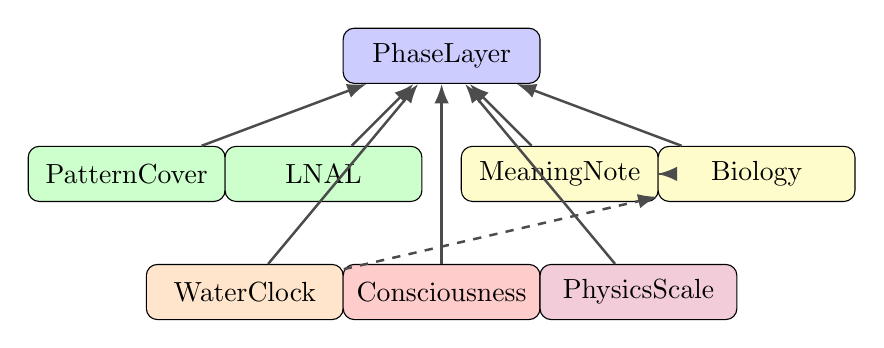
\begin{tikzpicture}[
  layer/.style={draw, rounded corners, minimum width=2.5cm, minimum height=0.7cm},
  arrow/.style={oct/arrow}
]
  % Core layers
  \node[layer, fill=blue!20] (phase) at (0, 0) {PhaseLayer};
  \node[layer, fill=green!20] (pattern) at (-4, -1.5) {PatternCover};
  \node[layer, fill=green!20] (lnal) at (-1.5, -1.5) {LNAL};
  \node[layer, fill=yellow!20] (meaning) at (1.5, -1.5) {MeaningNote};
  \node[layer, fill=yellow!20] (biology) at (4, -1.5) {Biology};
  
  % Lower layers
  \node[layer, fill=orange!20] (water) at (-2.5, -3) {WaterClock};
  \node[layer, fill=red!20] (consciousness) at (0, -3) {Consciousness};
  \node[layer, fill=purple!20] (physics) at (2.5, -3) {PhysicsScale};
  
  % Arrows to PhaseHub
  \draw[arrow] (pattern) -- (phase);
  \draw[arrow] (lnal) -- (phase);
  \draw[arrow] (meaning) -- (phase);
  \draw[arrow] (biology) -- (phase);
  \draw[arrow] (water) -- (phase);
  \draw[arrow] (consciousness) -- (phase);
  \draw[arrow] (physics) -- (phase);
  
  % Cross-layer dependencies
  \draw[arrow, dashed] (meaning) -- (biology);
  \draw[arrow, dashed] (water) -- (biology);
  
\end{tikzpicture}
\caption{Layer dependency graph. Solid arrows: bridges to PhaseHub. Dashed arrows: cross-layer dependencies.}
\end{figure}

\section{Bridge Network Summary}\label{app:bridges}

This appendix provides comprehensive documentation for the bridge network that connects all layers in the Octave System. Bridges are typed morphisms that preserve phase and commute with step functions.

% -----------------------------------------------------------------------------
% BRIDGE STRUCTURE
% -----------------------------------------------------------------------------
\subsection{Bridge Structure Definition}

\begin{definition}[Bridge]\label{def:bridge-full}
A bridge between layers $L_1$ and $L_2$ is a structure:
\begin{lstlisting}
structure Bridge (L1 L2 : Layer) where
  map : L1.State -> L2.State
  preservesPhase : forall s, L2.phase (map s) = L1.phase s
  commutesStep : forall s, map (L1.step s) = L2.step (map s)
\end{lstlisting}
\end{definition}

\subsubsection{Required Properties}

\begin{table}[H]
\centering
\begin{tabular}{lp{8cm}}
\toprule
\textbf{Property} & \textbf{Meaning} \\
\midrule
\texttt{map} & A function transforming source states to target states \\
\texttt{preservesPhase} & The phase of the mapped state equals the phase of the original \\
\texttt{commutesStep} & Mapping then stepping equals stepping then mapping \\
\bottomrule
\end{tabular}
\caption{Bridge structure components.}
\end{table}

\subsubsection{Diagram (Commutative Square)}

The \texttt{commutesStep} property states that this diagram commutes:

\begin{center}
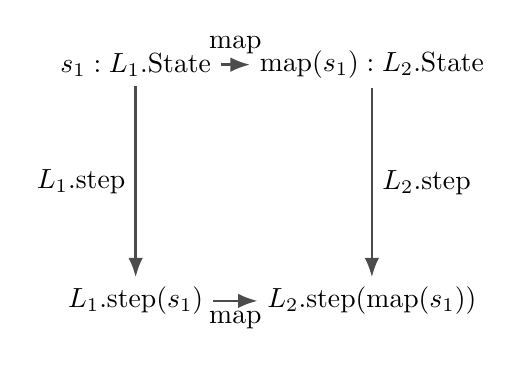
\begin{tikzpicture}[
  node distance=3cm,
  arrow/.style={oct/arrow}
]
  \node (s1) {$s_1 : L_1.\text{State}$};
  \node (s2) [right of=s1] {$\text{map}(s_1) : L_2.\text{State}$};
  \node (s1') [below of=s1] {$L_1.\text{step}(s_1)$};
  \node (s2') [below of=s2] {$L_2.\text{step}(\text{map}(s_1))$};
  
  \draw[arrow] (s1) -- node[above] {map} (s2);
  \draw[arrow] (s1) -- node[left] {$L_1$.step} (s1');
  \draw[arrow] (s2) -- node[right] {$L_2$.step} (s2');
  \draw[arrow] (s1') -- node[below] {map} (s2');
\end{tikzpicture}
\end{center}

% -----------------------------------------------------------------------------
% BRIDGE OPERATIONS
% -----------------------------------------------------------------------------
\subsection{Bridge Operations}

\subsubsection{Identity Bridge}

Every layer has an identity bridge to itself:
\begin{lstlisting}
def Bridge.id (L : Layer) : Bridge L L where
  map := id
  preservesPhase := fun _ => rfl
  commutesStep := fun _ => rfl
\end{lstlisting}

\subsubsection{Bridge Composition}

Bridges compose:
\begin{lstlisting}
def Bridge.comp (B1 : Bridge L1 L2) (B2 : Bridge L2 L3) : Bridge L1 L3 where
  map := B2.map circ B1.map
  preservesPhase := fun s => by
    simp [B2.preservesPhase, B1.preservesPhase]
  commutesStep := fun s => by
    simp [Function.comp, B1.commutesStep, B2.commutesStep]
\end{lstlisting}

\subsubsection{Composition Associativity}

\begin{theorem}[comp\_assoc]
Bridge composition is associative:
\[
  (B_1 \circ B_2) \circ B_3 = B_1 \circ (B_2 \circ B_3)
\]
\end{theorem}

\subsubsection{Iteration Theorems}

\begin{theorem}[phase\_iterate]
A bridge preserves phase after $n$ steps:
\[
  L_2.\text{phase}(\text{map}(L_1.\text{step}^n(s))) = L_1.\text{phase}(L_1.\text{step}^n(s))
\]
\end{theorem}

\begin{theorem}[map\_iterate]
Mapping commutes with iteration:
\[
  \text{map}(L_1.\text{step}^n(s)) = L_2.\text{step}^n(\text{map}(s))
\]
\end{theorem}

% ============================================================================
% FIGURE 5: BRIDGE COMPOSITION AND ITERATION (ENHANCED)
% ============================================================================
\begin{figure}[ht]
\centering
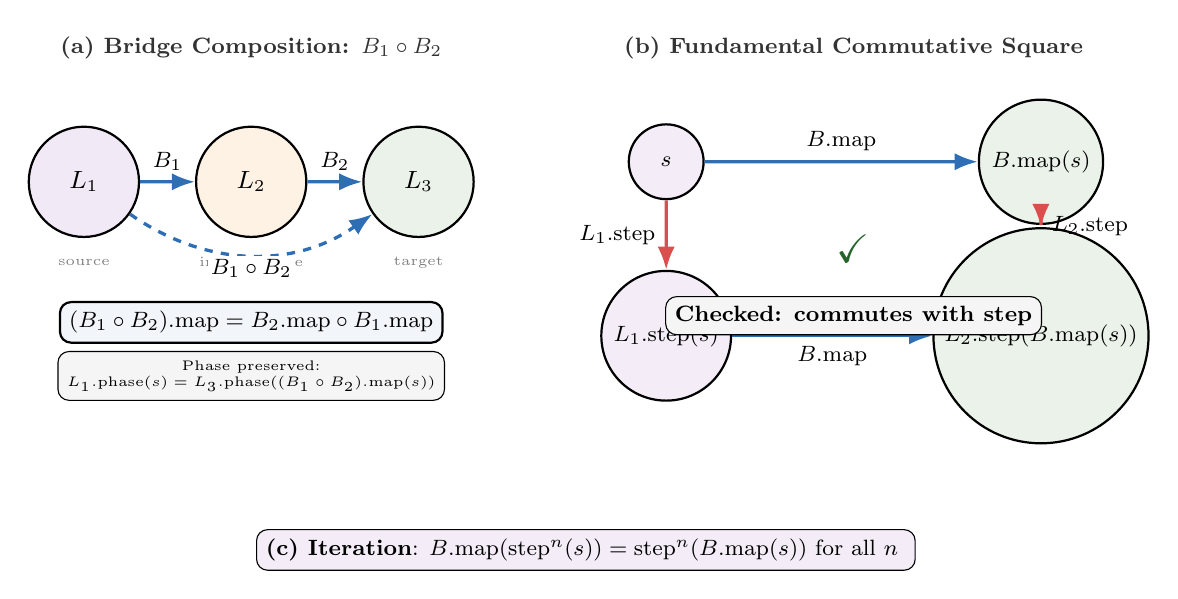
\begin{tikzpicture}[scale=0.85,
  layer/.style={draw, circle, minimum size=1.4cm, font=\small\bfseries, thick},
  state/.style={draw, circle, minimum size=0.95cm, font=\footnotesize, thick},
  arrow/.style={oct/arrow},
  bridge/.style={oct/bridge, line width=1.2pt},
  evolve/.style={oct/arrow, draw=octRed!85, line width=1.0pt},
  title/.style={font=\footnotesize\bfseries, text=black!80}
]

  % =========== (a) Bridge Composition ===========
  \node[title] at (-5, 5) {(a) Bridge Composition: $B_1 \circ B_2$};
  
  \node[layer, fill=octPurple!10] (L1) at (-7.5, 3) {$L_1$};
  \node[layer, fill=octOrange!10] (L2) at (-5, 3) {$L_2$};
  \node[layer, fill=octGreen!10] (L3) at (-2.5, 3) {$L_3$};
  
  % Layer labels
  \node[font=\tiny, gray] at (-7.5, 1.8) {source};
  \node[font=\tiny, gray] at (-5, 1.8) {intermediate};
  \node[font=\tiny, gray] at (-2.5, 1.8) {target};
  
  \draw[bridge] (L1) -- node[above, font=\footnotesize] {$B_1$} (L2);
  \draw[bridge] (L2) -- node[above, font=\footnotesize] {$B_2$} (L3);
  \draw[bridge, bend right=35, dashed] (L1) to node[below, font=\footnotesize, fill=white, inner sep=1pt] {$B_1 \circ B_2$} (L3);
  
  % Composition equation box
  \node[draw, rounded corners=4pt, fill=octBlue!6, font=\footnotesize, thick] at (-5, 0.9) {
    $(B_1 \circ B_2).\text{map} = B_2.\text{map} \circ B_1.\text{map}$
  };
  
  % Phase preservation annotation
  \node[draw, rounded corners, fill=octGray, font=\tiny, align=center] at (-5, 0.1) {
    Phase preserved:\\$L_1.\text{phase}(s) = L_3.\text{phase}((B_1\circ B_2).\text{map}(s))$
  };
  
  % =========== (b) Step/Map Commutativity ===========
  \node[title] at (4, 5) {(b) Fundamental Commutative Square};
  
  \node[state, fill=octPurple!8] (s1) at (1.2, 3.3) {$s$};
  \node[state, fill=octPurple!8] (s1step) at (1.2, 0.7) {$L_1.\text{step}(s)$};
  \node[state, fill=octGreen!10] (s2) at (6.8, 3.3) {$B.\text{map}(s)$};
  \node[state, fill=octGreen!10] (s2step) at (6.8, 0.7) {$L_2.\text{step}(B.\text{map}(s))$};
  
  \draw[evolve, line width=1.2pt] (s1) -- node[left, font=\footnotesize] {$L_1.\text{step}$} (s1step);
  \draw[bridge, line width=1.2pt] (s1) -- node[above, font=\footnotesize] {$B.\text{map}$} (s2);
  \draw[bridge, line width=1.2pt] (s1step) -- node[below, font=\footnotesize] {$B.\text{map}$} (s2step);
  \draw[evolve, line width=1.2pt] (s2) -- node[right, font=\footnotesize] {$L_2.\text{step}$} (s2step);
  
  % Commutes checkmark
  \node[font=\Large, octGreen!80!black] at (4, 2) {$\checkmark$};
  \node[draw, rounded corners, fill=octGray, font=\footnotesize\bfseries] at (4, 1) {Checked: commutes with step};
  
  % =========== (c) Iteration: simplified ===========
  \node[draw, rounded corners=4pt, fill=octPurple!8, font=\footnotesize, align=center] at (0, -2.5) {
    \textbf{(c) Iteration}: $B.\text{map}(\text{step}^n(s)) = \text{step}^n(B.\text{map}(s))$ for all $n$
  };
  
\end{tikzpicture}
\caption{\textbf{Figure 5: Bridge Composition and Commutativity.} (a) Bridges compose: $B_1 : L_1 \to L_2$ and $B_2 : L_2 \to L_3$ yield $B_1 \circ B_2 : L_1 \to L_3$. (b) The fundamental commutative diagram: map and step commute. (c) This extends to $n$ iterations.}
\label{fig:bridge-composition}
\end{figure}

% -----------------------------------------------------------------------------
% COMPLETE BRIDGE INVENTORY
% -----------------------------------------------------------------------------
\subsection{Complete Bridge Inventory}

\subsubsection{Core Bridges (to PhaseHub)}

\begin{table}[H]
\centering
\small
\begin{tabular}{llll}
\toprule
\textbf{Bridge Name} & \textbf{Source} & \textbf{Target} & \textbf{Map Function} \\
\midrule
\texttt{patternCoverToPhaseBridge} & PatternCoverLayer & PhaseLayer & \texttt{fun p => p} \\
\texttt{lnalToPhaseBridge} & LNALBreathLayer & PhaseLayer & \texttt{s.breath \% 8} \\
\texttt{meaningNoteToPhaseBridge} & MeaningNoteLayer & PhaseLayer & \texttt{s.tick \% 8} \\
\texttt{biologyToPhaseBridge} & BiologyQualiaLayer & PhaseLayer & \texttt{s.tick \% 8} \\
\texttt{waterClockToPhaseBridge} & WaterClockLayer & PhaseLayer & \texttt{s.bandIndex} \\
\texttt{consciousnessToPhaseBridge} & ConsciousnessPhaseLayer & PhaseLayer & \texttt{s.tick \% 8} \\
\texttt{physicsToPhaseBridge} & PhysicsScaleLayer & PhaseLayer & \texttt{s.rung} \\
\bottomrule
\end{tabular}
\caption{All seven projection bridges to PhaseHub.}
\label{tab:core-bridges}
\end{table}

\subsubsection{Named Cross-Layer Bridges (via PhaseLayer)}

\begin{table}[H]
\centering
\small
\begin{tabular}{lllp{5cm}}
\toprule
\textbf{Bridge Name} & \textbf{Source} & \textbf{Target} & \textbf{Description} \\
\midrule
\texttt{patternCoverToWaterClockBridge} & PatternCoverLayer & WaterClockLayer & Composition through PhaseLayer (phase-only) \\
\texttt{waterClockToPatternCoverBridge} & WaterClockLayer & PatternCoverLayer & Composition through PhaseLayer (phase-only) \\
\texttt{biologyToWaterClockBridge} & BiologyQualiaLayer & WaterClockLayer & $\pi_{\text{bio}}$ then \texttt{phaseToWaterClockBridge} \\
\texttt{consciousnessToPatternCoverBridge} & ConsciousnessPhaseLayer & PatternCoverLayer & $\pi_{\Theta}$ then \texttt{phaseToPatternCoverBridge} \\
\texttt{meaningNoteToWaterClockBridge} & MeaningNoteLayer & WaterClockLayer & $\pi_{\text{meaning}}$ then \texttt{phaseToWaterClockBridge} \\
\texttt{physicsToPatternCoverBridge} & PhysicsScaleLayer & PatternCoverLayer & $\pi_{\text{physics}}$ then \texttt{phaseToPatternCoverBridge} \\
\bottomrule
\end{tabular}
\caption{Named cross-layer bridges available in the reference implementation (conservative: they transport phase through PhaseLayer).}
\end{table}

\subsubsection{Derived Bridges (via Composition)}

The PhaseHub supports systematic derivations by composition. In particular, for any \StepAdvances{} layer $L$, composing the universal projection $\pi_L : L \to \PhaseLayer$ with a provided injection out of \PhaseLayer yields a derived bridge into an observation layer (e.g.\ WaterClock or PatternCover):
\begin{lstlisting}
-- Example (Lean-style): derive a bridge into WaterClockLayer via PhaseLayer
def L_to_Water (L : Layer) (hAdv : Layer.StepAdvances L) : Bridge L WaterClockLayer :=
  Bridge.comp (phaseProjectionBridge L hAdv) phaseToWaterClockBridge
\end{lstlisting}
\noindent\textbf{Note:} the hub always supports \emph{alignment checks} between any two layers (by comparing their projections into \PhaseLayer), but it does not automatically provide a bridge between arbitrary domain layers unless a suitable target-side injection is supplied.

% -----------------------------------------------------------------------------
% PHASEHUB ARCHITECTURE
% -----------------------------------------------------------------------------
\subsection{PhaseHub Architecture}

\subsubsection{Design Principle}

PhaseHub is the central coordination point:
\begin{itemize}
  \item Every domain layer has a projection to PhaseLayer
  \item Cross-domain connections go through PhaseHub
  \item This creates a ``star'' topology with PhaseLayer at center
\end{itemize}

\subsubsection{Network Diagram}

\begin{figure}[H]
\centering
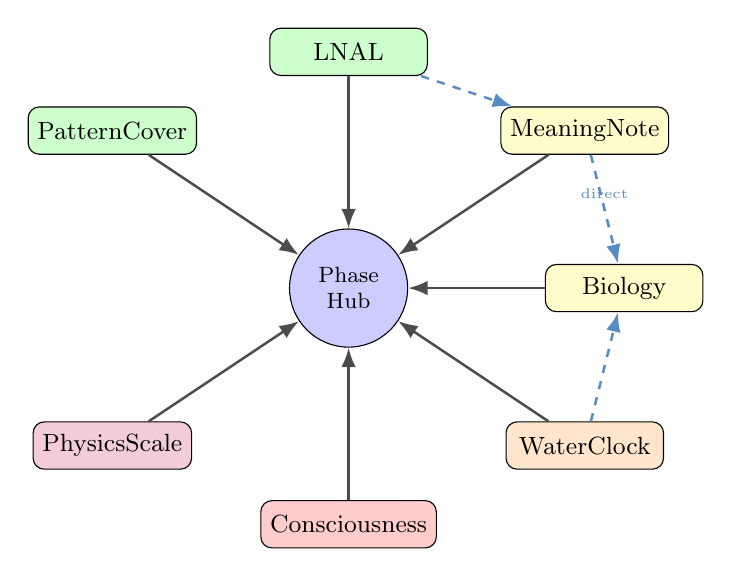
\begin{tikzpicture}[
  layer/.style={draw, rounded corners, minimum width=2cm, minimum height=0.6cm, font=\small},
  hub/.style={draw, circle, minimum size=1.5cm, fill=blue!20, font=\footnotesize, align=center},
  arrow/.style={oct/arrow}
]
  % Central hub
  \node[hub] (phase) at (0, 0) {Phase\\Hub};
  
  % Surrounding layers
  \node[layer, fill=green!20] (pattern) at (-3, 2) {PatternCover};
  \node[layer, fill=green!20] (lnal) at (0, 3) {LNAL};
  \node[layer, fill=yellow!20] (meaning) at (3, 2) {MeaningNote};
  \node[layer, fill=yellow!20] (biology) at (3.5, 0) {Biology};
  \node[layer, fill=orange!20] (water) at (3, -2) {WaterClock};
  \node[layer, fill=red!20] (consciousness) at (0, -3) {Consciousness};
  \node[layer, fill=purple!20] (physics) at (-3, -2) {PhysicsScale};
  
  % Arrows (bidirectional conceptually, shown as to-hub)
  \draw[arrow] (pattern) -- (phase);
  \draw[arrow] (lnal) -- (phase);
  \draw[arrow] (meaning) -- (phase);
  \draw[arrow] (biology) -- (phase);
  \draw[arrow] (water) -- (phase);
  \draw[arrow] (consciousness) -- (phase);
  \draw[arrow] (physics) -- (phase);
  
  % Some cross-domain arrows
  \draw[arrow, dashed, octBlue!80] (meaning) -- node[above, font=\tiny] {direct} (biology);
  \draw[arrow, dashed, octBlue!80] (water) -- (biology);
  \draw[arrow, dashed, octBlue!80] (lnal) -- (meaning);
  
\end{tikzpicture}
\caption{PhaseHub star topology. Solid arrows: projection bridges. Dashed arrows: cross-domain bridges.}
\end{figure}

\subsubsection{PhaseProjectionBridge}

The generic projection bridge from PhaseLayer to any layer:
\begin{lstlisting}
noncomputable def phaseProjectionBridge (L : Layer) 
    [StepAdvances L] : Bridge PhaseLayer L where
  map := fun p => -- find state with phase p
    Classical.choose (phase_surjective L p)
  preservesPhase := fun p => by
    simp [Classical.choose_spec (phase_surjective L p)]
  commutesStep := fun p => by
    -- uses StepAdvances to show step advances phase by 1
    ...
\end{lstlisting}

\subsubsection{Roundtrip Lemmas}

\begin{theorem}[roundtrip\_phase\_to\_layer\_to\_phase]
For any layer $L$ with \StepAdvances{}:
\[
  \text{phaseToLayer} \circ \text{layerToPhase} = \text{id} \quad \text{(on phases)}
\]
More precisely: the phase of the roundtrip equals the original phase.
\end{theorem}

\begin{theorem}[projection\_faithful]
Projection to PhaseHub is faithful on phases:
\[
  L.\text{phase}(s_1) = L.\text{phase}(s_2) \iff \text{toPhase}(s_1) = \text{toPhase}(s_2)
\]
\end{theorem}

% -----------------------------------------------------------------------------
% ALIGNMENT DEFINITIONS
% -----------------------------------------------------------------------------
\subsection{Alignment Definitions}

\subsubsection{Pairwise Alignment}

\begin{definition}[Aligned]
Two states from different layers are aligned if they have the same phase:
\begin{lstlisting}
def Aligned (L1 L2 : Layer) (s1 : L1.State) (s2 : L2.State) : Prop :=
  L1.phase s1 = L2.phase s2
\end{lstlisting}
\end{definition}

\subsubsection{Triple Alignment}

\begin{definition}[TriplyAligned]
Three states are triply aligned if all pairwise alignments hold:
\begin{lstlisting}
def TriplyAligned (L1 L2 L3 : Layer) 
    (s1 : L1.State) (s2 : L2.State) (s3 : L3.State) : Prop :=
  Aligned L1 L2 s1 s2 /\ Aligned L2 L3 s2 s3 /\ Aligned L1 L3 s1 s3
\end{lstlisting}
\end{definition}

\subsubsection{Universal Alignment}

\begin{definition}[UniversallyAligned]
A collection of layer-state pairs is universally aligned if all pairs are aligned:
\begin{lstlisting}
def UniversallyAligned (states : List (Sigma L : Layer, L.State)) : Prop :=
  forall (i j : Fin states.length), 
    let <L_i, s_i> := states[i]
    let <L_j, s_j> := states[j]
    Aligned L_i L_j s_i s_j
\end{lstlisting}
\end{definition}

% -----------------------------------------------------------------------------
% KEY THEOREMS
% -----------------------------------------------------------------------------
\subsection{Key Bridge Theorems}

\subsubsection{Alignment Preservation}

\begin{theorem}[aligned\_preserved\_by\_step]\label{thm:aligned-preserved}
If two states are aligned, they remain aligned after stepping:
\begin{lstlisting}
theorem aligned_preserved_by_step 
    (L1 L2 : Layer) [StepAdvances L1] [StepAdvances L2]
    (s1 : L1.State) (s2 : L2.State) 
    (hAligned : Aligned L1 L2 s1 s2) :
    Aligned L1 L2 (L1.step s1) (L2.step s2)
\end{lstlisting}
\end{theorem}

\begin{proof}
Both phases advance by 1, so the equality is preserved:
\begin{align*}
  L_1.\text{phase}(L_1.\text{step}(s_1)) &= L_1.\text{phase}(s_1) + 1 \\
  L_2.\text{phase}(L_2.\text{step}(s_2)) &= L_2.\text{phase}(s_2) + 1 \\
  &= L_1.\text{phase}(s_1) + 1 \quad \text{(by hAligned)}
\end{align*}
\end{proof}

\subsubsection{Iterated Alignment}

\begin{theorem}[aligned\_iterate]\label{thm:aligned-iterate}
Alignment is preserved for any number of steps:
\begin{lstlisting}
theorem aligned_iterate 
    (L1 L2 : Layer) [StepAdvances L1] [StepAdvances L2]
    (s1 : L1.State) (s2 : L2.State) (n : Nat)
    (hAligned : Aligned L1 L2 s1 s2) :
    Aligned L1 L2 (L1.step^[n] s1) (L2.step^[n] s2)
\end{lstlisting}
\end{theorem}

\subsubsection{Universal Synchronization}

\begin{theorem}[octave\_synchronization\_universal]\label{thm:universal-sync}
If a collection of states from layers with \StepAdvances{} is initially aligned, it remains aligned forever:
\begin{lstlisting}
theorem octave_synchronization_universal 
    (layers : List Layer) [forall L in layers, StepAdvances L]
    (states : forall L in layers, L.State)
    (hInitial : UniversallyAligned (zip layers states))
    (n : Nat) :
    UniversallyAligned (zip layers (map (step^[n]) states))
\end{lstlisting}
\end{theorem}

% -----------------------------------------------------------------------------
% BRIDGE STATISTICS
% -----------------------------------------------------------------------------
\subsection{Bridge Statistics}

\begin{table}[H]
\centering
\begin{tabular}{lr}
\toprule
\textbf{Metric} & \textbf{Count} \\
\midrule
Total layers & 8 \\
Projection bridges (to PhaseHub) & 7 \\
Cross-domain bridges (direct) & 4 \\
Identity bridges & 8 \\
Potential derived bridges & $7 \times 6 = 42$ \\
Bridges with proven \texttt{commutesStep} & 11 \\
Bridges marked \texttt{noncomputable} & 5 \\
\bottomrule
\end{tabular}
\caption{Bridge network statistics.}
\end{table}

% -----------------------------------------------------------------------------
% IMPLEMENTATION CHECKLIST
% -----------------------------------------------------------------------------
\subsection{Bridge Implementation Checklist}

When adding a new bridge, verify:

\begin{enumerate}
  \item \textbf{Define map function}: $L_1.\text{State} \to L_2.\text{State}$
  \item \textbf{Prove preservesPhase}: $\forall s, L_2.\text{phase}(\text{map}(s)) = L_1.\text{phase}(s)$
  \item \textbf{Prove commutesStep}: $\forall s, \text{map}(L_1.\text{step}(s)) = L_2.\text{step}(\text{map}(s))$
  \item \textbf{Add to bridge registry}: Update \texttt{OctaveKernel/Bridges.lean}
  \item \textbf{Verify composition}: Check that composition with existing bridges works
  \item \textbf{Document in paper}: Add to Table~\ref{tab:core-bridges}
\end{enumerate}

% -----------------------------------------------------------------------------
% SOURCE FILES
% -----------------------------------------------------------------------------
\subsection{Source Files}

\begin{table}[H]
\centering
\small
\begin{tabular}{lp{7cm}}
\toprule
\textbf{File} & \textbf{Contents} \\
\midrule
\texttt{OctaveKernel/Basic.lean} & \texttt{Bridge} structure, \texttt{Bridge.id}, \texttt{Bridge.comp} \\
\texttt{OctaveKernel/PhaseHub.lean} & \texttt{PhaseLayer}, \texttt{phaseProjectionBridge} \\
\texttt{OctaveKernel/Bridges/LayerProjections.lean} & All 7 projection bridges \\
\texttt{OctaveKernel/Bridges/CrossDomain.lean} & Cross-domain bridges \\
\texttt{OctaveKernel/Bridges/AlignmentTheorems.lean} & Alignment preservation theorems \\
\bottomrule
\end{tabular}
\caption{Source files for the bridge network.}
\end{table}

\section{LNAL Opcode Summary}\label{app:opcodes}

This appendix provides comprehensive documentation for the Light Native Assembly Language (LNAL), an 8-opcode virtual machine for semantic computation in the Octave System.

% -----------------------------------------------------------------------------
% OVERVIEW
% -----------------------------------------------------------------------------
\subsection{Overview}

\subsubsection{Purpose}

LNAL is the semantic layer's computational engine:
\begin{itemize}
  \item \textbf{8 opcodes}: Minimal instruction set for pattern manipulation
  \item \textbf{1024-tick breath}: Complete computation cycle
  \item \textbf{8-tick neutrality}: Ledger balances every 8 ticks
  \item \textbf{Invariant preservation}: All operations preserve key properties
\end{itemize}

\subsubsection{Design Philosophy}

\begin{itemize}
  \item \textbf{Minimality}: 8 opcodes suffice for all semantic operations
  \item \textbf{Symmetry}: Operations come in pairs (LOCK/FLIP, SEED/MERGE, etc.)
  \item \textbf{Conservation}: Token count and SU(3) charge are conserved
  \item \textbf{Phase alignment}: Breath cycle aligns with 8-tick structure
\end{itemize}

% -----------------------------------------------------------------------------
% SUMMARY TABLE
% -----------------------------------------------------------------------------
\subsection{Opcode Summary Table}

\begin{table}[H]
\centering
\begin{tabular}{clllc}
\toprule
\textbf{Code} & \textbf{Opcode} & \textbf{Effect} & \textbf{Key Invariant} & \textbf{Cost} \\
\midrule
0 & LOCK & Freeze phase state & SU3 & 1 \\
1 & BALANCE & Adjust token count & TokenParity & 1 \\
2 & FOLD & Propagate through network & SU3 & 2 \\
3 & SEED & Initialize new pattern & TokenParity & 1 \\
4 & BRAID & Weave adjacent states & SU3 & 2 \\
5 & MERGE & Combine recognition paths & TokenParity & 1 \\
6 & LISTEN & Await external input & All & 0 \\
7 & FLIP & Invert at breath midpoint & All & 0 \\
\bottomrule
\end{tabular}
\caption{LNAL opcode summary with numeric codes and costs.}
\label{tab:opcode-summary}
\end{table}

% -----------------------------------------------------------------------------
% DETAILED OPCODE SPECIFICATIONS
% -----------------------------------------------------------------------------
\subsection{Detailed Opcode Specifications}

% LOCK
\subsubsection{LOCK (0x00)}

\begin{table}[H]
\centering
\begin{tabular}{ll}
\toprule
\textbf{Property} & \textbf{Value} \\
\midrule
Mnemonic & \texttt{LOCK} \\
Numeric code & 0 \\
Arguments & \texttt{target : Reg6} \\
Effect & Prevents \texttt{target} register from changing \\
Cost & 1 \\
Invariants & Preserves SU3, may affect TokenParity \\
\bottomrule
\end{tabular}
\end{table}

\begin{lstlisting}
def execLock (s : LState) (target : Reg6) : LState :=
  { s with 
    reg6 := s.reg6.lock target,
    aux5 := { s.aux5 with phaseLock := true }
  }
\end{lstlisting}

\textbf{Semantics}: LOCK ``freezes'' the target register, preventing subsequent operations from modifying it until the next FLIP. Used to preserve critical values during computation.

% BALANCE
\subsubsection{BALANCE (0x01)}

\begin{table}[H]
\centering
\begin{tabular}{ll}
\toprule
\textbf{Property} & \textbf{Value} \\
\midrule
Mnemonic & \texttt{BALANCE} \\
Numeric code & 1 \\
Arguments & \texttt{mode : BalanceMode} \\
Effect & Adjusts token count and window sum \\
Cost & 1 \\
Invariants & Preserves TokenParity ($\in \{0, 1\}$) \\
\bottomrule
\end{tabular}
\end{table}

\begin{lstlisting}
inductive BalanceMode
  | inc    -- increment tokenCt (mod 2)
  | dec    -- decrement tokenCt (mod 2)
  | cycle  -- cycle window index, reset if needed

def execBalance (s : LState) (mode : BalanceMode) : LState :=
  match mode with
  | .inc => { s with aux5 := { s.aux5 with tokenCt := (s.aux5.tokenCt + 1) % 2 } }
  | .dec => { s with aux5 := { s.aux5 with tokenCt := (s.aux5.tokenCt + 1) % 2 } }
  | .cycle => 
    let newIdx := (s.winIdx8 + 1) % 8
    { s with winIdx8 := newIdx, winSum8 := if newIdx = 0 then 0 else s.winSum8 }
\end{lstlisting}

\textbf{Semantics}: BALANCE manages the token ledger. The \texttt{cycle} mode advances the 8-tick window and resets the sum at boundaries.

% FOLD
\subsubsection{FOLD (0x02)}

\begin{table}[H]
\centering
\begin{tabular}{ll}
\toprule
\textbf{Property} & \textbf{Value} \\
\midrule
Mnemonic & \texttt{FOLD} \\
Numeric code & 2 \\
Arguments & \texttt{depth : Nat} \\
Effect & Propagate value through $\phival$-hierarchy \\
Cost & 2 \\
Invariants & Preserves SU3 \\
\bottomrule
\end{tabular}
\end{table}

\begin{lstlisting}
def execFold (s : LState) (depth : Nat) : LState :=
  let newNuPhi := s.reg6.nuPhi + depth
  let newEll := s.reg6.ell * (depth + 1)
  { s with 
    reg6 := { s.reg6 with nuPhi := newNuPhi, ell := newEll },
    aux5 := { s.aux5 with neighborSum := s.aux5.neighborSum + depth }
  }
\end{lstlisting}

\textbf{Semantics}: FOLD propagates a pattern through the $\phival$-ladder by \texttt{depth} levels. This is the primary operation for hierarchical pattern processing.

% SEED
\subsubsection{SEED (0x03)}

\begin{table}[H]
\centering
\begin{tabular}{ll}
\toprule
\textbf{Property} & \textbf{Value} \\
\midrule
Mnemonic & \texttt{SEED} \\
Numeric code & 3 \\
Arguments & \texttt{pattern : Nat} \\
Effect & Initialize new pattern in registers \\
Cost & 1 \\
Invariants & Preserves TokenParity \\
\bottomrule
\end{tabular}
\end{table}

\begin{lstlisting}
def execSeed (s : LState) (pattern : Nat) : LState :=
  { s with 
    reg6 := { s.reg6 with 
      nuPhi := pattern % 4,
      tau := (pattern / 4) % 4,
      sigma := pattern % 256 - 128
    },
    aux5 := { s.aux5 with tokenCt := 1 }
  }
\end{lstlisting}

\textbf{Semantics}: SEED initializes a new pattern by distributing its bits across registers. Sets \texttt{tokenCt} to 1 (pattern present).

% BRAID
\subsubsection{BRAID (0x04)}

\begin{table}[H]
\centering
\begin{tabular}{ll}
\toprule
\textbf{Property} & \textbf{Value} \\
\midrule
Mnemonic & \texttt{BRAID} \\
Numeric code & 4 \\
Arguments & \texttt{offset : Int} \\
Effect & Weave with adjacent state at \texttt{offset} \\
Cost & 2 \\
Invariants & Preserves SU3 ($k_\perp \in \{-1, 0, +1\}$) \\
\bottomrule
\end{tabular}
\end{table}

\begin{lstlisting}
def execBraid (s : LState) (offset : Int) : LState :=
  let neighbor := s.mem.get! (s.ip + offset.toNat)
  let newKPerp := clampSU3 (s.reg6.kPerp + (if neighbor > 0 then 1 else -1))
  { s with 
    reg6 := { s.reg6 with kPerp := newKPerp },
    aux5 := { s.aux5 with neighborSum := s.aux5.neighborSum + neighbor }
  }
  where clampSU3 (k : Int) : Int := max (-1) (min 1 k)
\end{lstlisting}

\textbf{Semantics}: BRAID interleaves the current state with a neighbor at the given offset. The SU(3) charge $k_\perp$ is updated but clamped to $\{-1, 0, +1\}$.

% MERGE
\subsubsection{MERGE (0x05)}

\begin{table}[H]
\centering
\begin{tabular}{ll}
\toprule
\textbf{Property} & \textbf{Value} \\
\midrule
Mnemonic & \texttt{MERGE} \\
Numeric code & 5 \\
Arguments & \texttt{source : Reg6} \\
Effect & Combine \texttt{source} register into accumulator \\
Cost & 1 \\
Invariants & Preserves TokenParity \\
\bottomrule
\end{tabular}
\end{table}

\begin{lstlisting}
def execMerge (s : LState) (source : Reg6) : LState :=
  let sourceVal := s.reg6.get source
  { s with 
    reg6 := { s.reg6 with sigma := s.reg6.sigma + sourceVal },
    aux5 := { s.aux5 with tokenCt := (s.aux5.tokenCt + 1) % 2 }
  }
\end{lstlisting}

\textbf{Semantics}: MERGE combines the value from \texttt{source} register into the sigma accumulator. Token count toggles (preserving parity).

% LISTEN
\subsubsection{LISTEN (0x06)}

\begin{table}[H]
\centering
\begin{tabular}{ll}
\toprule
\textbf{Property} & \textbf{Value} \\
\midrule
Mnemonic & \texttt{LISTEN} \\
Numeric code & 6 \\
Arguments & None \\
Effect & Wait for external input (no-op in pure execution) \\
Cost & 0 \\
Invariants & Preserves all \\
\bottomrule
\end{tabular}
\end{table}

\begin{lstlisting}
def execListen (s : LState) : LState :=
  { s with aux5 := { s.aux5 with phaseLock := false } }
\end{lstlisting}

\textbf{Semantics}: LISTEN is a synchronization point. In pure execution, it simply releases any phase lock. In interactive mode, it waits for external input.

% FLIP
\subsubsection{FLIP (0x07)}

\begin{table}[H]
\centering
\begin{tabular}{ll}
\toprule
\textbf{Property} & \textbf{Value} \\
\midrule
Mnemonic & \texttt{FLIP} \\
Numeric code & 7 \\
Arguments & None \\
Effect & Invert phase, release locks \\
Cost & 0 \\
Invariants & Preserves all \\
Timing & Typically at breath tick 512 \\
\bottomrule
\end{tabular}
\end{table}

\begin{lstlisting}
def execFlip (s : LState) : LState :=
  { s with 
    reg6 := s.reg6.unlockAll,
    aux5 := { s.aux5 with 
      phaseLock := false,
      freeSlot := -s.aux5.freeSlot
    }
  }
\end{lstlisting}

\textbf{Semantics}: FLIP marks the midpoint of a breath cycle. It releases all locks and inverts the free slot (for symmetry). Occurs at tick 512 of 1024.

% -----------------------------------------------------------------------------
% STATE STRUCTURE
% -----------------------------------------------------------------------------
\subsection{State Structure}

\subsubsection{Complete LState}

\begin{lstlisting}
structure LState where
  -- Primary registers (6)
  reg6 : Reg6
  -- Auxiliary registers (5)
  aux5 : Aux5
  -- Breath cycle
  breath : Nat           -- tick within breath (0-1023)
  -- Execution control
  halted : Bool          -- has VM stopped?
  ip : Nat               -- instruction pointer
  -- Memory
  mem : Array Int        -- data memory
  -- 8-tick window tracking
  winIdx8 : Nat          -- index within current window (0-7)
  winSum8 : Int          -- sum over current window
\end{lstlisting}

\subsubsection{Primary Registers (Reg6)}

\begin{table}[H]
\centering
\begin{tabular}{llll}
\toprule
\textbf{Register} & \textbf{Type} & \textbf{Range} & \textbf{Description} \\
\midrule
\texttt{nuPhi} & \texttt{Nat} & $0, 1, 2, 3$ & $\phival$-level counter \\
\texttt{ell} & \texttt{Nat} & $\mathbb{N}$ & L-number (sequence position) \\
\texttt{sigma} & \texttt{Int} & $\mathbb{Z}$ & Signature accumulator \\
\texttt{tau} & \texttt{Nat} & $0, 2$ & Tau-offset ($\tau_0$ or $\tau_2$) \\
\texttt{kPerp} & \texttt{Int} & $-1, 0, +1$ & SU(3) generator \\
\texttt{phiE} & \texttt{Bool} & T/F & $\phival$-envelope flag \\
\bottomrule
\end{tabular}
\caption{Primary register set.}
\end{table}

\subsubsection{Auxiliary Registers (Aux5)}

\begin{table}[H]
\centering
\begin{tabular}{llll}
\toprule
\textbf{Register} & \textbf{Type} & \textbf{Range} & \textbf{Description} \\
\midrule
\texttt{neighborSum} & \texttt{Int} & $\mathbb{Z}$ & Neighbor interaction sum \\
\texttt{tokenCt} & \texttt{Nat} & $0, 1$ & Token count (parity) \\
\texttt{hydrationS} & \texttt{Nat} & $\mathbb{N}$ & Hydration state counter \\
\texttt{phaseLock} & \texttt{Bool} & T/F & Phase-locked indicator \\
\texttt{freeSlot} & \texttt{Int} & $\mathbb{Z}$ & General-purpose slot \\
\bottomrule
\end{tabular}
\caption{Auxiliary register set.}
\end{table}

% -----------------------------------------------------------------------------
% INVARIANTS
% -----------------------------------------------------------------------------
\subsection{Invariants}

\subsubsection{VMInvariant Bundle}

\begin{lstlisting}
def VMInvariant (s : LState) : Prop :=
  BreathBound s /\ 
  s.winIdx8 < 8 /\ 
  TokenParityInvariant s /\ 
  SU3Invariant s
\end{lstlisting}

\subsubsection{TokenParityInvariant}

\begin{lstlisting}
def TokenParityInvariant (s : LState) : Prop :=
  s.aux5.tokenCt in ({0, 1} : Set Nat)
\end{lstlisting}

\textbf{Meaning}: Token count is always 0 or 1. This models the presence/absence of a semantic token.

\subsubsection{SU3Invariant}

\begin{lstlisting}
def SU3Invariant (s : LState) : Prop :=
  s.reg6.kPerp in ({-1, 0, 1} : Set Int)
\end{lstlisting}

\textbf{Meaning}: The SU(3) charge is always in $\{-1, 0, +1\}$. This models color charge conservation.

\subsubsection{BreathBound}

\begin{lstlisting}
def BreathBound (s : LState) : Prop :=
  s.breath < 1024
\end{lstlisting}

\textbf{Meaning}: Breath tick is always within the 1024-tick cycle.

\subsubsection{8-Tick Neutrality}

\begin{lstlisting}
def Neutral8 (s : LState) : Prop :=
  s.winIdx8 = 7 -> s.winSum8 = 0
\end{lstlisting}

\textbf{Meaning}: At every 8th tick (when \texttt{winIdx8 = 7}), the window sum resets to 0.

% -----------------------------------------------------------------------------
% EXECUTION MODEL
% -----------------------------------------------------------------------------
\subsection{Execution Model}

\subsubsection{Single Step}

\begin{lstlisting}
def lStep (P : LProgram) (s : LState) : LState :=
  if s.halted then s
  else
    let instr := lFetch P s.ip
    let s' := lExec s instr
    { s' with 
      ip := s.ip + 1,
      breath := (s.breath + 1) % 1024
    }
\end{lstlisting}

\subsubsection{Instruction Fetch}

\begin{lstlisting}
def lFetch (P : LProgram) (ip : Nat) : Instruction :=
  if h : ip < P.length then P[ip] else Instruction.listen
\end{lstlisting}

If the IP exceeds program length, LISTEN is returned (safe default).

\subsubsection{Instruction Execute}

\begin{lstlisting}
def lExec (s : LState) (instr : Instruction) : LState :=
  match instr with
  | .lock target => execLock s target
  | .balance mode => execBalance s mode
  | .fold depth => execFold s depth
  | .seed pattern => execSeed s pattern
  | .braid offset => execBraid s offset
  | .merge source => execMerge s source
  | .listen => execListen s
  | .flip => execFlip s
\end{lstlisting}

% -----------------------------------------------------------------------------
% BREATH CYCLE
% -----------------------------------------------------------------------------
\subsection{Breath Cycle}

\subsubsection{Structure}

A complete breath cycle is 1024 ticks:

\begin{table}[H]
\centering
\begin{tabular}{cll}
\toprule
\textbf{Ticks} & \textbf{Phase} & \textbf{Description} \\
\midrule
0--511 & Inhale & Pattern accumulation \\
512 & FLIP & Midpoint inversion \\
513--1023 & Exhale & Pattern resolution \\
0 (wrap) & Reset & New breath begins \\
\bottomrule
\end{tabular}
\caption{Breath cycle phases.}
\end{table}

\subsubsection{8-Tick Windows}

Each breath contains $1024 / 8 = 128$ complete 8-tick windows.

\begin{center}
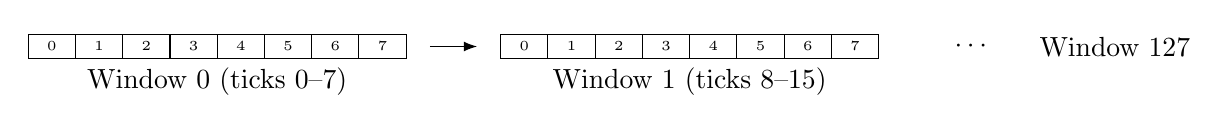
\begin{tikzpicture}[scale=0.6]
  % Draw 8-tick windows
  \foreach \i in {0,...,7} {
    \draw (\i, 0) rectangle (\i+1, 0.5);
    \node at (\i+0.5, 0.25) {\tiny \i};
  }
  \node at (4, -0.5) {Window 0 (ticks 0--7)};
  
  \draw[->] (8.5, 0.25) -- (9.5, 0.25);
  
  \foreach \i in {0,...,7} {
    \draw (\i+10, 0) rectangle (\i+11, 0.5);
    \node at (\i+10.5, 0.25) {\tiny \i};
  }
  \node at (14, -0.5) {Window 1 (ticks 8--15)};
  
  \node at (20, 0.25) {$\cdots$};
  
  \node at (23, 0.25) {Window 127};
\end{tikzpicture}
\end{center}

\subsubsection{Neutrality Theorem}

\begin{theorem}[neutral\_every\_8th\_from0]
At every 8-step boundary (i.e. when the window index has wrapped back to 0), the window sum is zero:
\[
  \forall k \in \mathbb{N}, \quad s^{[8k]}.\text{winIdx8}=0 \;\land\; s^{[8k]}.\text{winSum8} = 0
\]
where $s^{[n]}$ denotes $n$ steps from initial state $s$.
\end{theorem}

% -----------------------------------------------------------------------------
% EXAMPLE PROGRAMS
% -----------------------------------------------------------------------------
\subsection{Example Programs}

\subsubsection{Minimal Program (8 ticks)}

\begin{lstlisting}
def minimalProgram : LProgram := [
  .seed 42,       -- tick 0: initialize pattern
  .fold 1,        -- tick 1: propagate one level
  .balance .inc,  -- tick 2: increment token
  .braid 0,       -- tick 3: weave with self
  .listen,        -- tick 4: sync point
  .merge .sigma,  -- tick 5: merge accumulator
  .balance .dec,  -- tick 6: decrement token
  .flip           -- tick 7: end of window
]
\end{lstlisting}

\subsubsection{Full Breath Program}

\begin{lstlisting}
def breathProgram : LProgram :=
  -- 512 ticks: inhale phase
  List.replicate 64 minimalProgram |>.join ++
  -- 1 tick: flip
  [.flip] ++
  -- 511 ticks: exhale phase
  List.replicate 63 minimalProgram |>.join ++ [.listen, .listen, .listen, .listen, .listen, .listen, .listen]
\end{lstlisting}

\subsubsection{Invariant Test}

\begin{lstlisting}
-- Verify VMInvariant after 8 ticks
example : VMInvariant (lStep^[8] minimalProgram initialState) := by
  native_decide
\end{lstlisting}

% -----------------------------------------------------------------------------
% COST MODEL
% -----------------------------------------------------------------------------
\subsection{Cost Model}

\subsubsection{Opcode Costs}

\begin{lstlisting}
def instrCost (instr : Instruction) : Nat :=
  match instr with
  | .lock _ => 1
  | .balance _ => 1
  | .fold _ => 2
  | .seed _ => 1
  | .braid _ => 2
  | .merge _ => 1
  | .listen => 0
  | .flip => 0
\end{lstlisting}

\subsubsection{Cost Rationale}

\begin{itemize}
  \item \textbf{FOLD, BRAID}: Cost 2 (involve $\phival$-hierarchy or neighbor access)
  \item \textbf{LOCK, BALANCE, SEED, MERGE}: Cost 1 (local register operations)
  \item \textbf{LISTEN, FLIP}: Cost 0 (synchronization, no computation)
\end{itemize}

\subsubsection{Total Cost Bound}

\begin{theorem}[instrCost\_bounded]
For any instruction, $\text{instrCost}(\text{instr}) \le 2$.
\end{theorem}

% -----------------------------------------------------------------------------
% SOURCE FILES
% -----------------------------------------------------------------------------
\subsection{Source Files}

\begin{table}[H]
\centering
\small
\begin{tabular}{lp{7cm}}
\toprule
\textbf{File} & \textbf{Contents} \\
\midrule
\texttt{LNAL/Opcodes.lean} & \texttt{Opcode} inductive, \texttt{Instruction} structure \\
\texttt{LNAL/Registers.lean} & \texttt{Reg6}, \texttt{Aux5} structures \\
\texttt{LNAL/VM.lean} & \texttt{LState}, \texttt{lStep}, \texttt{lFetch}, \texttt{lExec} \\
\texttt{LNAL/Invariants.lean} & VMInvariant, TokenParity, SU3, neutrality theorems \\
\texttt{LNAL/InstrCost.lean} & \texttt{instrCost}, cost bounds \\
\texttt{LNAL/JBudget.lean} & J-budget tracking, cost accumulation \\
\texttt{LNAL/Tests.lean} & Example programs, property tests \\
\bottomrule
\end{tabular}
\caption{LNAL source files.}
\end{table}

\section{Build Instructions}\label{app:build}

This appendix provides comprehensive instructions for building, verifying, and developing with the Octave System codebase.

% -----------------------------------------------------------------------------
% SYSTEM REQUIREMENTS
% -----------------------------------------------------------------------------
\subsection{System Requirements}

\subsubsection{Hardware}

\begin{table}[H]
\centering
\begin{tabular}{lll}
\toprule
\textbf{Component} & \textbf{Minimum} & \textbf{Recommended} \\
\midrule
RAM & 8 GB & 16 GB \\
Storage & 5 GB free & 10 GB free \\
CPU & Dual-core & Quad-core \\
\bottomrule
\end{tabular}
\caption{Hardware requirements.}
\end{table}

\textbf{Note}: Full builds can be memory-intensive. Close other applications if you encounter out-of-memory errors.

\subsubsection{Operating System}

\begin{itemize}
  \item \textbf{macOS}: 12.0 (Monterey) or later
  \item \textbf{Linux}: Ubuntu 20.04+, Debian 11+, or equivalent
  \item \textbf{Windows}: WSL2 with Ubuntu recommended (native Windows is experimental)
\end{itemize}

\subsubsection{Software Prerequisites}

\begin{table}[H]
\centering
\begin{tabular}{llp{6cm}}
\toprule
\textbf{Software} & \textbf{Version} & \textbf{Notes} \\
\midrule
\Lean{} & pinned by \texttt{lean-toolchain} & Managed by \texttt{elan} \\
Lake & (bundled with \Lean{}) & Build system \\
Mathlib & (via \texttt{lakefile.lean}) & Mathematical library \\
Git & 2.30+ & Version control \\
curl & any & For \texttt{elan} installation \\
\bottomrule
\end{tabular}
\caption{Software prerequisites.}
\end{table}

% -----------------------------------------------------------------------------
% INSTALLATION
% -----------------------------------------------------------------------------
\subsection{Installation}

\subsubsection{Step 1: Install elan (Lean Version Manager)}

\begin{lstlisting}[language=bash, frame=none, backgroundcolor=\color{white}]
# Install elan (manages Lean versions)
curl https://raw.githubusercontent.com/leanprover/elan/master/elan-init.sh -sSf | sh

# Follow the prompts, then reload your shell
source ~/.profile  # or ~/.bashrc, ~/.zshrc
\end{lstlisting}

Verify installation:
\begin{lstlisting}[language=bash, frame=none, backgroundcolor=\color{white}]
elan --version
# Expected: elan 3.x.x

lean --version
# Expected: Lean (version 4.x.x, ...)
\end{lstlisting}

\subsubsection{Step 2: Clone the Repository}

\begin{lstlisting}[language=bash, frame=none, backgroundcolor=\color{white}]
git clone https://github.com/jonwashburn/reality
cd reality
\end{lstlisting}

\subsubsection{Step 3: Configure Lean Toolchain}

The repository includes a \texttt{lean-toolchain} file that specifies the exact \Lean{} version:
\begin{lstlisting}[language=bash, frame=none, backgroundcolor=\color{white}]
cat lean-toolchain
# Output: leanprover/lean4:v4.26.0-rc2
\end{lstlisting}

\texttt{elan} will automatically use this version when you're in the project directory.

\subsubsection{Step 4: Fetch Dependencies}

\begin{lstlisting}[language=bash, frame=none, backgroundcolor=\color{white}]
lake update
\end{lstlisting}

This downloads Mathlib and other dependencies. First run may take 10--30 minutes.

\subsubsection{Step 5: Build the Project}

\begin{lstlisting}[language=bash, frame=none, backgroundcolor=\color{white}]
lake build
\end{lstlisting}

\textbf{Expected time}: 15--60 minutes (first build). Subsequent builds are incremental.

% -----------------------------------------------------------------------------
% BUILD COMMANDS
% -----------------------------------------------------------------------------
\subsection{Build Commands}

\subsubsection{Full Build}

\begin{lstlisting}[language=bash, frame=none, backgroundcolor=\color{white}]
lake build
\end{lstlisting}

Builds all modules. Use for final verification.

\subsubsection{Scoped Build (Single Module)}

\begin{lstlisting}[language=bash, frame=none, backgroundcolor=\color{white}]
# Build the Octave-facing certificate bundle (recommended for refereeing)
lake build IndisputableMonolith.Octave.Bundle

# Build only the OctaveKernel module
lake build IndisputableMonolith.OctaveKernel

# Build only the LNAL VM
lake build IndisputableMonolith.LNAL.VM

# Build integration tests
lake build IndisputableMonolith.OctaveKernel.IntegrationTests
\end{lstlisting}

Scoped builds are faster for development.

\subsubsection{Clean Build}

\begin{lstlisting}[language=bash, frame=none, backgroundcolor=\color{white}]
lake clean
lake build
\end{lstlisting}

Use if you encounter strange errors after updating.

\subsubsection{Update Dependencies}

\begin{lstlisting}[language=bash, frame=none, backgroundcolor=\color{white}]
lake update
lake build
\end{lstlisting}

Fetches latest compatible versions of dependencies.

% -----------------------------------------------------------------------------
% VERIFICATION
% -----------------------------------------------------------------------------
\subsection{Verification Commands}

\subsubsection{Check for Sorry Holes}

\begin{lstlisting}[language=bash, frame=none, backgroundcolor=\color{white}]
grep -r "\\bsorry\\b" IndisputableMonolith --include="*.lean" | grep -v "-- sorry"
\end{lstlisting}

\textbf{Note}: whether this is 0 depends on the audit scope. For repo-wide counts, see \texttt{artifacts/reality\_audit.json}; for the Octave-facing surface, the intent is \texttt{sorry}-free certificates.

\subsubsection{Count Axioms}

\begin{lstlisting}[language=bash, frame=none, backgroundcolor=\color{white}]
grep -r "^axiom\\|^  axiom" IndisputableMonolith --include="*.lean" | wc -l
\end{lstlisting}

\textbf{Note}: counts depend on what you include/exclude (Mathlib, archived files, documentation). For an explicit audit under a chosen scope, see \texttt{artifacts/axiom\_audit.json} and \texttt{artifacts/reality\_audit.json}.

\subsubsection{List Hypothesis Axioms}

\begin{lstlisting}[language=bash, frame=none, backgroundcolor=\color{white}]
grep -r "axiom H_" IndisputableMonolith --include="*.lean"
\end{lstlisting}

Lists all hypothesis axioms (empirical claims awaiting validation).

\subsubsection{Verify Specific Theorem}

\begin{lstlisting}[language=bash, frame=none, backgroundcolor=\color{white}]
# Type-check a single file
lake env lean IndisputableMonolith/OctaveKernel/Basic.lean
\end{lstlisting}

\subsubsection{Run Example Proofs}

\begin{lstlisting}[language=bash, frame=none, backgroundcolor=\color{white}]
lake build IndisputableMonolith.Sonification.Examples
\end{lstlisting}

% -----------------------------------------------------------------------------
% PROJECT STRUCTURE
% -----------------------------------------------------------------------------
\subsection{Project Structure}

\begin{lstlisting}[frame=none, backgroundcolor=\color{white}]
reality/                      # Lean project root
|-- lakefile.lean             # Build configuration
|-- lean-toolchain            # Lean version (elan-managed)
|-- IndisputableMonolith/
|   |-- Octave/               # Paper-facing bundle exports
|   |-- OctaveKernel/         # Core framework + instances + bridges
|   |-- LNAL/                 # Virtual machine + invariants
|   |-- Water/                # WToken↔AminoAcid certificates
|   |-- Sonification/         # Sonification model + examples
|-- book/docs/                # Paper sources (this .tex)
|-- artifacts/                # Audit JSONs (sorries/axioms/etc.)
\end{lstlisting}

\subsubsection{Key Directories}

\begin{table}[H]
\centering
\small
\begin{tabular}{lp{8cm}}
\toprule
\textbf{Directory} & \textbf{Contents} \\
\midrule
\texttt{OctaveKernel/} & Core \texttt{Layer} and \texttt{Bridge} definitions, PhaseHub \\
\texttt{OctaveKernel/Instances/} & All 8 layer implementations \\
\texttt{OctaveKernel/Bridges/} & Bridge implementations and alignment theorems \\
\texttt{LNAL/} & Light Native Assembly Language VM \\
\texttt{Water/} & WToken definitions and bijection proofs \\
\texttt{Sonification/} & Audio mapping, consonance metrics \\
\texttt{BiophaseCore/} & Water/BIOPHASE constants \\
\texttt{Consciousness/} & Speculative consciousness models \\
\texttt{Verification/} & Meta-theorems, necessity proofs \\
\bottomrule
\end{tabular}
\caption{Key directories and their contents.}
\end{table}

% -----------------------------------------------------------------------------
% EDITOR SETUP
% -----------------------------------------------------------------------------
\subsection{Editor Setup (VS Code)}

\subsubsection{Install VS Code Extensions}

\begin{enumerate}
  \item Install VS Code: \url{https://code.visualstudio.com/}
  \item Install the \textbf{lean4} extension (by leanprover)
  \item Restart VS Code
\end{enumerate}

\subsubsection{Open the Project}

\begin{lstlisting}[language=bash, frame=none, backgroundcolor=\color{white}]
code .
\end{lstlisting}

\subsubsection{Useful Keybindings}

\begin{table}[H]
\centering
\begin{tabular}{ll}
\toprule
\textbf{Action} & \textbf{Keybinding} \\
\midrule
Go to Definition & F12 \\
Hover for Type & Ctrl/Cmd + K, Ctrl/Cmd + I \\
Show Goal State & (automatic in tactic mode) \\
Restart Lean Server & Ctrl/Cmd + Shift + P $\to$ ``Lean: Restart'' \\
\bottomrule
\end{tabular}
\caption{VS Code keybindings for Lean.}
\end{table}

\subsubsection{Infoview Panel}

The Lean Infoview panel (right side) shows:
\begin{itemize}
  \item Current goal state during proofs
  \item Type of expression under cursor
  \item Error messages
\end{itemize}

% -----------------------------------------------------------------------------
% TROUBLESHOOTING
% -----------------------------------------------------------------------------
\subsection{Troubleshooting}

\subsubsection{``lake build'' Hangs or Times Out}

\textbf{Cause}: Full build is memory-intensive.

\textbf{Solution}: Use scoped builds:
\begin{lstlisting}[language=bash, frame=none, backgroundcolor=\color{white}]
lake build IndisputableMonolith.OctaveKernel.Basic
\end{lstlisting}

\subsubsection{``Unknown identifier'' Errors}

\textbf{Cause}: Missing import.

\textbf{Solution}: Add the appropriate import at the top of the file:
\begin{lstlisting}
import IndisputableMonolith.OctaveKernel.Basic
\end{lstlisting}

\subsubsection{``Type mismatch'' Errors}

\textbf{Cause}: Expression has wrong type.

\textbf{Solution}: Use \texttt{\#check expr} to see the actual type, then adjust.

\subsubsection{Mathlib API Changes}

\textbf{Cause}: Mathlib function was renamed or moved.

\textbf{Solution}: 
\begin{enumerate}
  \item Check Mathlib changelog
  \item Search Mathlib docs for the new name
  \item Update the import or function call
\end{enumerate}

\subsubsection{``Noncomputable'' Errors}

\textbf{Cause}: Definition uses classical logic or real numbers.

\textbf{Solution}: Mark the definition as \texttt{noncomputable}:
\begin{lstlisting}
noncomputable def myFunction : Real := ...
\end{lstlisting}

\subsubsection{Out of Memory}

\textbf{Cause}: Build requires more RAM.

\textbf{Solution}:
\begin{enumerate}
  \item Close other applications
  \item Use scoped builds
  \item Increase swap space (Linux)
\end{enumerate}

% -----------------------------------------------------------------------------
% CI/CD PIPELINE
% -----------------------------------------------------------------------------
\subsection{Continuous Integration}

\subsubsection{GitHub Actions Workflow}

The repository includes CI workflows under \texttt{.github/workflows/} (e.g. \texttt{ci.yml}):

\begin{lstlisting}[language=bash, frame=none, backgroundcolor=\color{white}]
# (illustrative) build + certificate checks
- uses: actions/checkout@v4
- uses: leanprover/lean-action@v1
- run: lake build
- run: lake env lean --run CI/Checks.lean
\end{lstlisting}

\subsubsection{CI Checks}

Every commit triggers:
\begin{enumerate}
  \item Full \texttt{lake build} (must pass)
  \item Sorry/axiom audits (thresholds depend on the chosen audit scope; see \texttt{artifacts/reality\_audit.json})
\end{enumerate}

\subsubsection{Pull Request Requirements}

Before merging:
\begin{itemize}
  \item All CI checks pass
  \item No new \texttt{sorry} holes
  \item New axioms documented
  \item Code review approved
\end{itemize}

% -----------------------------------------------------------------------------
% DEVELOPMENT WORKFLOW
% -----------------------------------------------------------------------------
\subsection{Development Workflow}

\subsubsection{Adding a New Theorem}

\begin{enumerate}
  \item Create or edit the \texttt{.lean} file
  \item Write the theorem statement
  \item Start with \texttt{sorry} placeholder
  \item Build to check types: \texttt{lake build ModuleName}
  \item Replace \texttt{sorry} with actual proof
  \item Verify: \texttt{lake build}
\end{enumerate}

\subsubsection{Adding a New Layer}

\begin{enumerate}
  \item Create \texttt{OctaveKernel/Instances/MyLayer.lean}
  \item Define state type
  \item Implement \texttt{Layer} structure
  \item Prove \texttt{StepAdvances}
  \item Create bridge to PhaseHub
  \item Add import to \texttt{OctaveKernel.lean}
  \item Run integration tests
\end{enumerate}

\subsubsection{Running Tests}

\begin{lstlisting}[language=bash, frame=none, backgroundcolor=\color{white}]
# Unit tests
lake build IndisputableMonolith.LNAL.Tests

# Integration tests
lake build IndisputableMonolith.OctaveKernel.IntegrationTests

# Property tests
lake build IndisputableMonolith.Sonification.Examples
\end{lstlisting}

% -----------------------------------------------------------------------------
% QUICK REFERENCE
% -----------------------------------------------------------------------------
\subsection{Quick Reference}

\begin{table}[H]
\centering
\begin{tabular}{lp{8cm}}
\toprule
\textbf{Task} & \textbf{Command} \\
\midrule
Full build & \texttt{cd reality \&\& lake build} \\
Scoped build & \texttt{lake build IndisputableMonolith.Module} \\
Clean build & \texttt{lake clean \&\& lake build} \\
Update deps & \texttt{lake update} \\
Sorry audit & \texttt{grep -r "sorry" ... | grep -v "-- sorry"} \\
Axiom count & \texttt{grep -r "\^{}axiom" ... | wc -l} \\
Type-check file & \texttt{lake env lean path/to/file.lean} \\
\bottomrule
\end{tabular}
\caption{Build command quick reference.}
\end{table}

% ============================================================================
% APPENDIX E: COMPLETE WTOKEN CLASSIFICATION
% ============================================================================
\section{Complete WToken Classification}\label{app:wtoken}

This appendix provides comprehensive documentation for the 20 WTokens---the semantic atoms of the Octave System. Each WToken corresponds bijectively to one of the 20 amino acids, establishing a bridge between meaning and biology.

% -----------------------------------------------------------------------------
% OVERVIEW
% -----------------------------------------------------------------------------
\subsection{Overview}

\subsubsection{What Are WTokens?}

WTokens are \textbf{semantic primitives}---fundamental units of meaning in the Light Language framework. They are classified by three parameters derived from the 8-tick structure:

\begin{enumerate}
  \item \textbf{DFT-8 Mode Family}: Which conjugate pair of Fourier modes (1+7, 2+6, 3+5, or 4)
  \item \textbf{$\phival$-Level}: Scale position in the golden ratio hierarchy (0, 1, 2, or 3)
  \item \textbf{$\tau$-Offset}: Phase offset (0 or 2, mode-4 only)
\end{enumerate}

\subsubsection{Why 20?}

The number 20 arises from the structure of DFT-8:
\begin{align}
  \text{Total} &= \underbrace{4}_{\text{mode (1+7)}} + \underbrace{4}_{\text{mode (2+6)}} + \underbrace{4}_{\text{mode (3+5)}} + \underbrace{4 \times 2}_{\text{mode (4) with } \tau} \\
  &= 4 + 4 + 4 + 8 = 20
\end{align}

This exactly matches the 20 standard amino acids---a correspondence we formalize and prove.

% -----------------------------------------------------------------------------
% CLASSIFICATION PARAMETERS
% -----------------------------------------------------------------------------
\subsection{Classification Parameters}

\subsubsection{DFT-8 Mode Families}

The Discrete Fourier Transform over 8 points produces frequency bins $k = 0, 1, \ldots, 7$. Excluding the DC ($k=0$) mode, the remaining 7 bins form 4 conjugate-pair families:

\begin{table}[H]
\centering
\begin{tabular}{clccp{5cm}}
\toprule
\textbf{Family} & \textbf{Modes} & \textbf{Frequency} & \textbf{Tokens} & \textbf{Character} \\
\midrule
$(1+7)$ & $k=1, k=7$ & Lowest & 4 & Fundamental, ground, foundation \\
$(2+6)$ & $k=2, k=6$ & Low & 4 & Relational, interactive, dynamic \\
$(3+5)$ & $k=3, k=5$ & Medium & 4 & Receptive, cyclical, balanced \\
$(4)$ & $k=4$ & Nyquist & 8 & Central, polar, complete \\
\bottomrule
\end{tabular}
\caption{DFT-8 mode families with frequency interpretation.}
\end{table}

\textbf{Why conjugate pairs?} For real-valued signals, $X_k = \overline{X_{8-k}}$. Modes $(k)$ and $(8-k)$ carry the same information, so we group them.

\subsubsection{$\phival$-Levels}

Each mode family has 4 $\phival$-levels representing scale hierarchy:

\begin{table}[H]
\centering
\begin{tabular}{cccl}
\toprule
\textbf{Level} & \textbf{Factor} & \textbf{Decimal} & \textbf{Interpretation} \\
\midrule
0 & $\phival^0$ & 1.000 & Ground state, origin, seed \\
1 & $\phival^1$ & 1.618 & First emergence, differentiation \\
2 & $\phival^2$ & 2.618 & Developed structure, elaboration \\
3 & $\phival^3$ & 4.236 & Full expression, culmination \\
\bottomrule
\end{tabular}
\caption{The four $\phival$-levels and their interpretations.}
\end{table}

\textbf{Why 4 levels?} The $\phival$-ladder is infinite, but we truncate at level 3 because:
\begin{itemize}
  \item $4 \times 4 + 4 \times 2 = 20$ matches biology
  \item Level 4+ would require additional structure not seen in amino acids
\end{itemize}

\subsubsection{$\tau$-Offset (Mode-4 Only)}

The central mode $(k=4)$ is self-conjugate and has a symmetry that allows two phase variants:

\begin{table}[H]
\centering
\begin{tabular}{cll}
\toprule
\textbf{Offset} & \textbf{Value} & \textbf{Interpretation} \\
\midrule
$\tau_0$ & 0 & Symmetric, in-phase, stable \\
$\tau_2$ & 2 & Antisymmetric, quarter-cycle, dynamic \\
\bottomrule
\end{tabular}
\caption{The two $\tau$-offsets for mode-4 tokens.}
\end{table}

This doubles mode-4 tokens: $4 \times 2 = 8$, bringing the total to 20.

% -----------------------------------------------------------------------------
% LEAN DEFINITIONS
% -----------------------------------------------------------------------------
\subsection{Lean Definitions}

\subsubsection{Mode Type}

\begin{lstlisting}
inductive WTokenMode : Type
  | mode1_7  -- (1+7)
  | mode2_6  -- (2+6)
  | mode3_5  -- (3+5)
  | mode4    -- (4)
deriving DecidableEq, Repr
\end{lstlisting}

\subsubsection{$\phival$-Level and $\tau$-Offset}

\begin{lstlisting}
inductive PhiLevel : Type
  | level0 | level1 | level2 | level3
deriving DecidableEq, Repr

inductive TauOffset : Type
  | tau0 | tau2
deriving DecidableEq, Repr
\end{lstlisting}

\subsubsection{WToken Structure}

\begin{lstlisting}
structure WTokenSpec where
  mode : WTokenMode
  phi_level : PhiLevel
  tau_offset : TauOffset
  -- Non-mode4 tokens must have tau0.
  tau_valid : mode ≠ WTokenMode.mode4 → tau_offset = TauOffset.tau0 := by decide
deriving Repr

def WToken : Type := WTokenSpec
\end{lstlisting}

The \texttt{tau\_valid} constraint ensures that only mode-4 tokens use $\tau_2$.

\subsubsection{All 20 WTokens}

\begin{lstlisting}
def allWTokens : List WTokenSpec := [
  W0_Origin, W1_Emergence, W2_Polarity, W3_Harmony,
  W4_Power, W5_Birth, W6_Structure, W7_Resonance,
  W8_Infinity, W9_Truth, W10_Completion, W11_Inspire,
  W12_Transform, W13_End, W14_Connection, W15_Wisdom,
  W16_Illusion, W17_Chaos, W18_Twist, W19_Time
]

theorem wtoken_count : allWTokens.length = 20 := by native_decide
\end{lstlisting}

% -----------------------------------------------------------------------------
% COMPLETE WTOKEN TABLE
% -----------------------------------------------------------------------------
\subsection{Complete WToken Table}

\begin{longtable}{clcccp{3.5cm}l}
\toprule
\textbf{\#} & \textbf{Name} & \textbf{Mode} & \textbf{$\phival$} & \textbf{$\tau$} & \textbf{Meaning} & \textbf{Amino Acid} \\
\midrule
\endfirsthead
\toprule
\textbf{\#} & \textbf{Name} & \textbf{Mode} & \textbf{$\phival$} & \textbf{$\tau$} & \textbf{Meaning} & \textbf{Amino Acid} \\
\midrule
\endhead
\midrule
\multicolumn{7}{r}{\textit{Continued on next page}} \\
\endfoot
\bottomrule
\endlastfoot
\multicolumn{7}{c}{\textbf{Mode (1+7): Fundamental --- Ground Layer}} \\
\midrule
W0 & Origin & 1+7 & 0 & -- & The void, potentiality & Glycine (G) \\
W1 & Emergence & 1+7 & 1 & -- & First distinction, birth & Alanine (A) \\
W2 & Polarity & 1+7 & 2 & -- & Movement, process & Valine (V) \\
W3 & Harmony & 1+7 & 3 & -- & Form, pattern, order & Leucine (L) \\
\midrule
\multicolumn{7}{c}{\textbf{Mode (2+6): Relational --- Interaction Layer}} \\
\midrule
W4 & Power & 2+6 & 0 & -- & Connection, bond & Serine (S) \\
W5 & Birth & 2+6 & 1 & -- & Metamorphosis & Threonine (T) \\
W6 & Structure & 2+6 & 2 & -- & Unification, synthesis & Asparagine (N) \\
W7 & Resonance & 2+6 & 3 & -- & Manifestation, output & Glutamine (Q) \\
\midrule
\multicolumn{7}{c}{\textbf{Mode (3+5): Receptive --- Sensitivity Layer}} \\
\midrule
W8 & Infinity & 3+5 & 0 & -- & Input, sensing & Aspartic Acid (D) \\
W9 & Truth & 3+5 & 1 & -- & Equilibrium, harmony & Glutamic Acid (E) \\
W10 & Completion & 3+5 & 2 & -- & Return, rhythm & Lysine (K) \\
W11 & Inspire & 3+5 & 3 & -- & Interior, profound & Arginine (R) \\
\midrule
\multicolumn{7}{c}{\textbf{Mode (4): Central --- Axis Layer}} \\
\midrule
W12 & Transform-$\tau_0$ & 4 & 0 & 0 & Stillness, pivot & Histidine (H) \\
W13 & End-$\tau_0$ & 4 & 1 & 0 & Polarity, duality & Phenylalanine (F) \\
W14 & Connection-$\tau_0$ & 4 & 2 & 0 & Vibration, attunement & Tyrosine (Y) \\
W15 & Wisdom-$\tau_0$ & 4 & 3 & 0 & Interference, coupling & Tryptophan (W) \\
W16 & Illusion-$\tau_2$ & 4 & 0 & 2 & Consonance, alignment & Proline (P) \\
W17 & Chaos-$\tau_2$ & 4 & 1 & 2 & Dissonance, tension & Cysteine (C) \\
W18 & Twist-$\tau_2$ & 4 & 2 & 2 & Fulfillment, wholeness & Methionine (M) \\
W19 & Time-$\tau_2$ & 4 & 3 & 2 & Duration, eternity & Isoleucine (I) \\
\end{longtable}

% -----------------------------------------------------------------------------
% BINARY ENCODING
% -----------------------------------------------------------------------------
\subsection{Binary Encoding}

Each WToken can be encoded as a 5-bit codeword (interpretable as an integer in $0..31$, with gaps):

\begin{table}[H]
\centering
\small
\begin{tabular}{cccccl}
\toprule
\textbf{WToken} & \textbf{Binary} & \textbf{Mode bits} & \textbf{$\phival$ bits} & \textbf{$\tau$ bit} & \textbf{Amino} \\
\midrule
W0 & 00000 & 00 & 00 & 0 & Gly \\
W1 & 00010 & 00 & 01 & 0 & Ala \\
W2 & 00100 & 00 & 10 & 0 & Val \\
W3 & 00110 & 00 & 11 & 0 & Leu \\
W4 & 01000 & 01 & 00 & 0 & Ser \\
W5 & 01010 & 01 & 01 & 0 & Thr \\
W6 & 01100 & 01 & 10 & 0 & Asn \\
W7 & 01110 & 01 & 11 & 0 & Gln \\
W8 & 10000 & 10 & 00 & 0 & Asp \\
W9 & 10010 & 10 & 01 & 0 & Glu \\
W10 & 10100 & 10 & 10 & 0 & Lys \\
W11 & 10110 & 10 & 11 & 0 & Arg \\
W12 & 11000 & 11 & 00 & 0 & His \\
W13 & 11010 & 11 & 01 & 0 & Phe \\
W14 & 11100 & 11 & 10 & 0 & Tyr \\
W15 & 11110 & 11 & 11 & 0 & Trp \\
W16 & 11001 & 11 & 00 & 1 & Pro \\
W17 & 11011 & 11 & 01 & 1 & Cys \\
W18 & 11101 & 11 & 10 & 1 & Met \\
W19 & 11111 & 11 & 11 & 1 & Ile \\
\bottomrule
\end{tabular}
\caption{5-bit binary encoding of WTokens.}
\end{table}

\textbf{Encoding scheme}:
\begin{itemize}
  \item Bits 4--3: Mode (00 = 1+7, 01 = 2+6, 10 = 3+5, 11 = 4)
  \item Bits 2--1: $\phival$-level (00, 01, 10, 11)
  \item Bit 0: $\tau$-offset (0 = $\tau_0$, 1 = $\tau_2$, only used for mode 4)
\end{itemize}

% -----------------------------------------------------------------------------
% BIJECTION PROOF
% -----------------------------------------------------------------------------
\subsection{WToken--AminoAcid Bijection}

\subsubsection{Amino Acid Type}

\begin{lstlisting}
inductive AminoAcid : Type
  | Gly | Ala | Val | Leu | Ile
  | Phe | Trp | Tyr
  | Ser | Thr | Asn | Gln | Cys | Met
  | Lys | Arg | His | Asp | Glu | Pro
deriving DecidableEq, Repr, Fintype
\end{lstlisting}

\subsubsection{Forward Mapping}

\begin{lstlisting}
def wtoken_to_amino : WTokenSpec → AminoAcid
  | ⟨.mode1_7, .level0, _, _⟩ => .Gly
  | ⟨.mode1_7, .level1, _, _⟩ => .Ala
  | ⟨.mode1_7, .level2, _, _⟩ => .Val
  | ⟨.mode1_7, .level3, _, _⟩ => .Leu
  | ⟨.mode2_6, .level0, _, _⟩ => .Ser
  | ⟨.mode2_6, .level1, _, _⟩ => .Thr
  | ⟨.mode2_6, .level2, _, _⟩ => .Asn
  | ⟨.mode2_6, .level3, _, _⟩ => .Gln
  | ⟨.mode3_5, .level0, _, _⟩ => .Asp
  | ⟨.mode3_5, .level1, _, _⟩ => .Glu
  | ⟨.mode3_5, .level2, _, _⟩ => .Lys
  | ⟨.mode3_5, .level3, _, _⟩ => .Arg
  | ⟨.mode4, .level0, .tau0, _⟩ => .His
  | ⟨.mode4, .level1, .tau0, _⟩ => .Phe
  | ⟨.mode4, .level2, .tau0, _⟩ => .Tyr
  | ⟨.mode4, .level3, .tau0, _⟩ => .Trp
  | ⟨.mode4, .level0, .tau2, _⟩ => .Pro
  | ⟨.mode4, .level1, .tau2, _⟩ => .Cys
  | ⟨.mode4, .level2, .tau2, _⟩ => .Met
  | ⟨.mode4, .level3, .tau2, _⟩ => .Ile
\end{lstlisting}

\subsubsection{Inverse Mapping}

\begin{lstlisting}
def amino_to_wtoken : AminoAcid → WTokenSpec
  | .Gly => W0_Origin
  | .Ala => W1_Emergence
  | .Val => W2_Polarity
  | .Leu => W3_Harmony
  | .Ser => W4_Power
  | .Thr => W5_Birth
  | .Asn => W6_Structure
  | .Gln => W7_Resonance
  | .Asp => W8_Infinity
  | .Glu => W9_Truth
  | .Lys => W10_Completion
  | .Arg => W11_Inspire
  | .His => W12_Transform
  | .Phe => W13_End
  | .Tyr => W14_Connection
  | .Trp => W15_Wisdom
  | .Pro => W16_Illusion
  | .Cys => W17_Chaos
  | .Met => W18_Twist
  | .Ile => W19_Time
\end{lstlisting}

\subsubsection{Bijection Theorem}

\begin{theorem}[wtoken\_amino\_bijection]
The mappings \texttt{wtoken\_to\_amino} and \texttt{amino\_to\_wtoken} form a bijection:
\begin{lstlisting}
theorem wtoken_amino_bijection : Function.Bijective wtoken_to_amino :=
  wtoken_amino_equiv.bijective
\end{lstlisting}
\end{theorem}

\subsubsection{Equivalence}

\begin{lstlisting}
def wtoken_amino_equiv : WTokenSpec ≃ AminoAcid :=
{ toFun := wtoken_to_amino
, invFun := amino_to_wtoken
, left_inv := wtoken_to_amino_leftInverse
, right_inv := wtoken_to_amino_rightInverse
}
\end{lstlisting}

% -----------------------------------------------------------------------------
% SEMANTIC-CHEMICAL CORRESPONDENCES
% -----------------------------------------------------------------------------
\subsection{Semantic-Chemical Correspondences}

Beyond the formal bijection, there are striking semantic correspondences:

\subsubsection{Mode (1+7): Foundation}

\begin{table}[H]
\centering
\begin{tabular}{llp{6cm}}
\toprule
\textbf{WToken} & \textbf{Amino Acid} & \textbf{Correspondence} \\
\midrule
W0: Origin & Glycine & Smallest AA, fits anywhere---like the void \\
W1: Emergence & Alanine & Simplest side chain (CH$_3$)---first distinction \\
W2: Polarity & Valine & Hydrophobic, branched---polarity boundary and flow \\
W3: Harmony & Leucine & Hydrophobic core builder---harmonizing structure \\
\bottomrule
\end{tabular}
\end{table}

\subsubsection{Mode (2+6): Interaction}

\begin{table}[H]
\centering
\begin{tabular}{llp{6cm}}
\toprule
\textbf{WToken} & \textbf{Amino Acid} & \textbf{Correspondence} \\
\midrule
W4: Power & Serine & Hydroxyl for H-bonding---power to connect \\
W5: Birth & Threonine & Hydroxyl + methyl---growth of complexity \\
W6: Structure & Asparagine & Amide group---structure via H-bond networks \\
W7: Resonance & Glutamine & Larger amide---resonant polar interactions \\
\bottomrule
\end{tabular}
\end{table}

\subsubsection{Mode (3+5): Sensitivity}

\begin{table}[H]
\centering
\begin{tabular}{llp{6cm}}
\toprule
\textbf{WToken} & \textbf{Amino Acid} & \textbf{Correspondence} \\
\midrule
W8: Infinity & Aspartic Acid & Negative charge---unbounded interaction potential \\
W9: Truth & Glutamic Acid & Negative charge---stable electrostatic ``law'' \\
W10: Completion & Lysine & Positive charge---closing/completing interactions \\
W11: Inspire & Arginine & Strong positive charge---binding/catalytic ``inspiration'' \\
\bottomrule
\end{tabular}
\end{table}

\subsubsection{Mode (4): Center}

\begin{table}[H]
\centering
\begin{tabular}{llp{6cm}}
\toprule
\textbf{WToken} & \textbf{Amino Acid} & \textbf{Correspondence} \\
\midrule
W12: Transform ($\tau_0$) & Histidine & Imidazole switching---transformative chemistry \\
W13: End ($\tau_0$) & Phenylalanine & Aromatic packing---terminal hydrophobic core \\
W14: Connection ($\tau_0$) & Tyrosine & Phosphorylation site---connects signaling cascades \\
W15: Wisdom ($\tau_0$) & Tryptophan & Largest aromatic---information-rich / rare \\
W16: Illusion ($\tau_2$) & Proline & Helix breaker---kinks and ``illusions'' in structure \\
W17: Chaos ($\tau_2$) & Cysteine & Disulfide/redox---order from chaos \\
W18: Twist ($\tau_2$) & Methionine & Start codon (AUG)---turning point / twist \\
W19: Time ($\tau_2$) & Isoleucine & Hydrophobic core---stability over time \\
\bottomrule
\end{tabular}
\end{table}

% -----------------------------------------------------------------------------
% SONIFICATION MAPPING
% -----------------------------------------------------------------------------
\subsection{Sonification Mapping}

WTokens map to musical pitches for protein sonification:

\begin{table}[H]
\centering
\small
\begin{tabular}{cllcc}
\toprule
\textbf{WToken} & \textbf{Base Pitch} & \textbf{Octave Shift} & \textbf{MIDI} & \textbf{Note} \\
\midrule
W0--W3 & C (60) & $\phival$-level $\times$ 12 & 60, 72, 84, 96 & C4--C7 \\
W4--W7 & E (64) & $\phival$-level $\times$ 12 & 64, 76, 88, 100 & E4--E7 \\
W8--W11 & G (67) & $\phival$-level $\times$ 12 & 67, 79, 91, 103 & G4--G7 \\
W12--W19 & B$\flat$ (70) & $\phival$-level $\times$ 12 $\pm$ 6 & varies & B$\flat$4+ \\
\bottomrule
\end{tabular}
\caption{Base pitches for WToken sonification.}
\end{table}

Mode-4 tokens with $\tau_2$ offset add a tritone (+6 semitones) for dissonance.

% -----------------------------------------------------------------------------
% CODON ASSOCIATIONS
% -----------------------------------------------------------------------------
\subsection{Representative Codons}

Each WToken/AminoAcid has multiple codons. Here are representatives:

\begin{table}[H]
\centering
\small
\begin{tabular}{clll}
\toprule
\textbf{W\#} & \textbf{Amino Acid} & \textbf{Codons} & \textbf{Representative} \\
\midrule
W0 & Glycine & GGU, GGC, GGA, GGG & GGU \\
W1 & Alanine & GCU, GCC, GCA, GCG & GCU \\
W18 & Methionine & AUG (only) & AUG \\
W17 & Cysteine & UGU, UGC & UGU \\
W15 & Tryptophan & UGG (only) & UGG \\
\bottomrule
\end{tabular}
\caption{Sample codon associations (complete table in MeaningNoteLayer).}
\end{table}

% -----------------------------------------------------------------------------
% SOURCE FILES
% -----------------------------------------------------------------------------
\subsection{Source Files}

\begin{table}[H]
\centering
\small
\begin{tabular}{lp{7cm}}
\toprule
\textbf{File} & \textbf{Contents} \\
\midrule
\texttt{IndisputableMonolith/Water/WTokenIso.lean} & WTokenSpec, AminoAcid, explicit maps \texttt{wtoken\_to\_amino}/\texttt{amino\_to\_wtoken}, and the packaged equivalence \texttt{wtoken\_amino\_equiv}. \\
\texttt{IndisputableMonolith/LightLanguage/WTokens.lean} & Compatibility aliases re-exporting the Water namespace as \texttt{LightLanguage.WTokens}. \\
\texttt{IndisputableMonolith/Genetics/Basic.lean} & Codons + universal genetic code definition (DNA/RNA alphabet conventions). \\
\texttt{IndisputableMonolith/Genetics/MeaningNote.lean} & The \texttt{MeaningNote} artifact bundling a WToken, amino acid, codon, and decoding witness. \\
\texttt{IndisputableMonolith/OctaveKernel/Instances/MeaningNoteLayer.lean} & Conservative Octave \texttt{Layer} witness carrying \texttt{MeaningNote} across an 8-phase tick. \\
\texttt{IndisputableMonolith/Sonification/Basic.lean} & Pitch mapping functions for WToken-driven sonification. \\
\bottomrule
\end{tabular}
\caption{WToken-related source files.}
\end{table}

% ============================================================================
% APPENDIX F: DETAILED LNAL SEMANTICS
% ============================================================================
\section{Detailed LNAL Opcode Semantics}\label{app:lnal-semantics}

This appendix provides complete formal specifications for the Light Native Assembly Language (LNAL) virtual machine, including register architecture, opcode semantics, execution model, and invariant preservation proofs.

% -----------------------------------------------------------------------------
% OVERVIEW
% -----------------------------------------------------------------------------
\subsection{Overview}

\subsubsection{Design Goals}

LNAL is designed to:
\begin{enumerate}
  \item \textbf{Minimal}: 8 opcodes are sufficient for semantic computation
  \item \textbf{Symmetric}: Operations come in complementary pairs
  \item \textbf{Invariant-preserving}: Key properties hold across all executions
  \item \textbf{Phase-aligned}: 8-tick structure matches the Octave framework
\end{enumerate}

\subsubsection{Architecture Summary}

\begin{table}[H]
\centering
\begin{tabular}{ll}
\toprule
\textbf{Component} & \textbf{Specification} \\
\midrule
Opcodes & 8 (LOCK, BALANCE, FOLD, SEED, BRAID, MERGE, LISTEN, FLIP) \\
Primary registers & 6 (Reg6) \\
Auxiliary registers & 5 (Aux5) \\
Breath cycle & 1024 ticks \\
Window size & 8 ticks \\
Memory model & Array of integers \\
\bottomrule
\end{tabular}
\caption{LNAL architecture summary.}
\end{table}

% -----------------------------------------------------------------------------
% REGISTER ARCHITECTURE
% -----------------------------------------------------------------------------
\subsection{Register Architecture}

\subsubsection{Core Registers (Reg6)}

The primary register file contains 6 registers for semantic computation:

\begin{table}[H]
\centering
\begin{tabular}{llccp{5cm}}
\toprule
\textbf{Register} & \textbf{Type} & \textbf{Init} & \textbf{Range} & \textbf{Description} \\
\midrule
$\nu_\phi$ (\texttt{nuPhi}) & Nat & 0 & $\mathbb{N}$ & $\phival$-phase accumulator \\
$\ell$ (\texttt{ell}) & Nat & 0 & $\mathbb{N}$ & Length/extent register \\
$\sigma$ (\texttt{sigma}) & Int & 0 & $\mathbb{Z}$ & Signature hash accumulator \\
$\tau$ (\texttt{tau}) & Nat & 0 & $\{0, 2\}$ & Time/offset register \\
$k_\perp$ (\texttt{kPerp}) & Int & 0 & $\{-1, 0, +1\}$ & SU(3) generator \\
$\phi_E$ (\texttt{phiE}) & Bool & false & $\{\text{T}, \text{F}\}$ & Energy envelope flag \\
\bottomrule
\end{tabular}
\caption{Core LNAL registers with initial values and ranges.}
\end{table}

\textbf{Lean definition}:
\begin{lstlisting}
structure Reg6 where
  nuPhi : Nat := 0
  ell : Nat := 0
  sigma : Int := 0
  tau : Nat := 0
  kPerp : Int := 0
  phiE : Bool := false
\end{lstlisting}

\subsubsection{Auxiliary Registers (Aux5)}

The auxiliary register file contains 5 registers for state tracking:

\begin{table}[H]
\centering
\begin{tabular}{llccp{5cm}}
\toprule
\textbf{Register} & \textbf{Type} & \textbf{Init} & \textbf{Range} & \textbf{Description} \\
\midrule
neighborSum & Int & 0 & $\mathbb{Z}$ & Neighbor interaction sum \\
tokenCt & Nat & 0 & $\{0, 1\}$ & Token count (parity) \\
hydrationS & Nat & 0 & $\mathbb{N}$ & Hydration state \\
phaseLock & Bool & false & $\{\text{T}, \text{F}\}$ & Phase lock flag \\
freeSlot & Int & 0 & $\mathbb{Z}$ & General-purpose temp \\
\bottomrule
\end{tabular}
\caption{Auxiliary LNAL registers with initial values and ranges.}
\end{table}

\textbf{Lean definition}:
\begin{lstlisting}
structure Aux5 where
  neighborSum : Int := 0
  tokenCt : Nat := 0
  hydrationS : Nat := 0
  phaseLock : Bool := false
  freeSlot : Int := 0
\end{lstlisting}

\subsubsection{Complete State (LState)}

\begin{lstlisting}
structure LState where
  reg6 : Reg6              -- Primary registers
  aux5 : Aux5              -- Auxiliary registers
  breath : Nat := 0        -- Tick within breath (0-1023)
  halted : Bool := false   -- Execution stopped?
  ip : Nat := 0            -- Instruction pointer
  mem : Array Int := #[]   -- Data memory
  winIdx8 : Nat := 0       -- Index within 8-tick window
  winSum8 : Int := 0       -- Sum over current window
\end{lstlisting}

% -----------------------------------------------------------------------------
% INSTRUCTION FORMAT
% -----------------------------------------------------------------------------
\subsection{Instruction Format}

\subsubsection{Instruction Structure}

\begin{lstlisting}
structure Instruction where
  opcode : Opcode          -- Which operation
  arg : OpcodeArg          -- Opcode-specific argument
\end{lstlisting}

\subsubsection{Opcode Enumeration}

\begin{lstlisting}
inductive Opcode where
  | lock    : Opcode  -- 0x00
  | balance : Opcode  -- 0x01
  | fold    : Opcode  -- 0x02
  | seed    : Opcode  -- 0x03
  | braid   : Opcode  -- 0x04
  | merge   : Opcode  -- 0x05
  | listen  : Opcode  -- 0x06
  | flip    : Opcode  -- 0x07
\end{lstlisting}

\subsubsection{Argument Types}

\begin{lstlisting}
inductive OpcodeArg where
  | none : OpcodeArg                        -- LOCK, LISTEN, FLIP
  | balance : BalanceMode -> OpcodeArg       -- BALANCE
  | fold : Nat -> OpcodeArg                  -- FOLD depth
  | seed : Nat -> OpcodeArg                  -- SEED pattern
  | braid : Int -> OpcodeArg                 -- BRAID offset
  | merge : Reg6Field -> OpcodeArg           -- MERGE source

inductive BalanceMode where
  | inc | dec | cycle | reset
\end{lstlisting}

% -----------------------------------------------------------------------------
% EXECUTION MODEL
% -----------------------------------------------------------------------------
\subsection{Execution Model}

\subsubsection{Single Step (lStep)}

\begin{lstlisting}
def lStep (P : LProgram) (s : LState) : LState :=
  if s.halted then s
  else
    let instr := lFetch P s.ip
    let s' := lExec s instr
    { s' with 
      breath := (s.breath + 1) % breathPeriod,  -- 1024
      winIdx8 := (s.winIdx8 + 1) % 8 }
\end{lstlisting}

\subsubsection{Instruction Fetch}

\begin{lstlisting}
def lFetch (P : LProgram) (ip : Nat) : Instruction :=
  if h : ip < P.length then 
    P[ip]
  else 
    <.listen, .none>  -- Default: LISTEN (safe no-op)
\end{lstlisting}

\subsubsection{Instruction Dispatch}

\begin{lstlisting}
def lExec (s : LState) (instr : Instruction) : LState :=
  match instr.opcode, instr.arg with
  | .lock, _ => execLOCK s
  | .balance, .balance mode => execBALANCE s mode
  | .fold, .fold depth => execFOLD s depth
  | .seed, .seed pattern => execSEED s pattern
  | .braid, .braid offset => execBRAID s offset
  | .merge, .merge source => execMERGE s source
  | .listen, _ => execLISTEN s
  | .flip, _ => execFLIP s
  | _, _ => s  -- Invalid: no-op
\end{lstlisting}

\subsubsection{State Machine Diagram}

\begin{center}
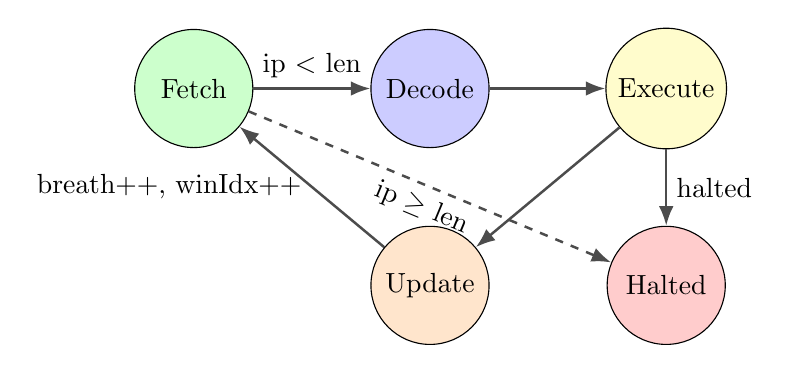
\begin{tikzpicture}[
  state/.style={draw, circle, minimum size=1.5cm},
  arrow/.style={oct/arrow}
]
  \node[state, fill=green!20] (fetch) at (0, 0) {Fetch};
  \node[state, fill=blue!20] (decode) at (3, 0) {Decode};
  \node[state, fill=yellow!20] (exec) at (6, 0) {Execute};
  \node[state, fill=orange!20] (update) at (3, -2.5) {Update};
  \node[state, fill=red!20] (halt) at (6, -2.5) {Halted};
  
  \draw[arrow] (fetch) -- node[above] {ip $<$ len} (decode);
  \draw[arrow] (decode) -- (exec);
  \draw[arrow] (exec) -- (update);
  \draw[arrow] (update) -- node[left] {breath++, winIdx++} (fetch);
  \draw[arrow] (exec) -- node[right] {halted} (halt);
  \draw[arrow, dashed] (fetch) -- node[below, sloped] {ip $\ge$ len} (halt);
\end{tikzpicture}
\end{center}

% -----------------------------------------------------------------------------
% 8-TICK WINDOW MECHANICS
% -----------------------------------------------------------------------------
\subsection{8-Tick Window Mechanics}

\subsubsection{Window State}

Each state tracks its position within an 8-tick window:
\begin{itemize}
  \item \texttt{winIdx8}: Current index (0--7)
  \item \texttt{winSum8}: Accumulated sum over window
\end{itemize}

\subsubsection{Window Cycle}

\begin{lstlisting}
-- After each step:
winIdx8 := (winIdx8 + 1) % 8
-- When winIdx8 wraps to 0, winSum8 should be 0 (neutrality)
\end{lstlisting}

\subsubsection{Neutrality Invariant}

At every 8th tick, the window sum resets:
\begin{lstlisting}
def Neutral8 (s : LState) : Prop :=
  s.winIdx8 = 7 -> s.winSum8 = 0
\end{lstlisting}

\textbf{Theorem}: If neutral at start, neutral at every boundary.

\begin{figure}[H]
\centering
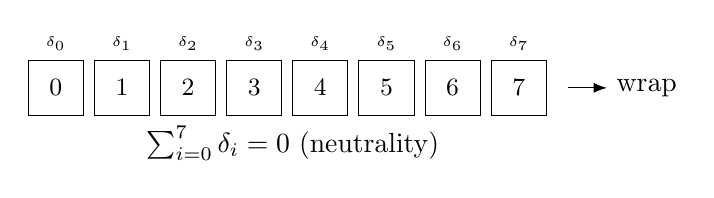
\begin{tikzpicture}[scale=0.7]
  % Window visualization
  \foreach \i in {0,...,7} {
    \draw (\i*1.2, 0) rectangle (\i*1.2+1, 1);
    \node at (\i*1.2+0.5, 0.5) {\small \i};
    \node at (\i*1.2+0.5, 1.3) {\tiny $\delta_\i$};
  }
  \node at (4.8, -0.5) {$\sum_{i=0}^{7} \delta_i = 0$ (neutrality)};
  \draw[->] (9.8, 0.5) -- (10.5, 0.5) node[right] {wrap};
\end{tikzpicture}
\caption{8-tick window with neutrality constraint.}
\end{figure}

% -----------------------------------------------------------------------------
% BREATH CYCLE MECHANICS
% -----------------------------------------------------------------------------
\subsection{Breath Cycle Mechanics}

\subsubsection{Cycle Structure}

A complete breath is 1024 ticks, divided into:

\begin{table}[H]
\centering
\begin{tabular}{cclp{5cm}}
\toprule
\textbf{Phase} & \textbf{Ticks} & \textbf{Name} & \textbf{Description} \\
\midrule
Inhale & 0--511 & Accumulation & Gather patterns, build recognition \\
Flip & 512 & Midpoint & FLIP opcode inverts state \\
Exhale & 513--1023 & Resolution & Resolve patterns, output results \\
\bottomrule
\end{tabular}
\caption{Breath cycle phases.}
\end{table}

\subsubsection{Windows Per Breath}

\[
  \frac{1024 \text{ ticks}}{8 \text{ ticks/window}} = 128 \text{ windows per breath}
\]

\subsubsection{FLIP Timing}

FLIP occurs at tick 512:
\begin{lstlisting}
def shouldFlip (s : LState) : Bool := s.breath = 512
\end{lstlisting}

\subsection{Opcode Specifications}

\subsubsection{LOCK}

\begin{lstlisting}
def execLOCK (s : LState) (arg : OpcodeArg) : LState :=
  { s with phaseLock := true, ip := s.ip + 1 }
\end{lstlisting}

\begin{description}
  \item[Effect] Sets \texttt{phaseLock} to true, freezing phase state.
  \item[Invariants] Preserves SU3 ($k_\perp$ unchanged), preserves TokenParity.
  \item[Use case] Synchronization point before cross-layer communication.
\end{description}

\subsubsection{BALANCE}

\begin{lstlisting}
def execBALANCE (s : LState) (mode : BalanceMode) : LState :=
  match mode with
  | .reset => { s with tokenCt := 0, winSum8 := 0, ip := s.ip + 1 }
  | .incr  => { s with tokenCt := clamp01 (s.tokenCt + 1), ip := s.ip + 1 }
  | .decr  => { s with tokenCt := clamp01 (s.tokenCt - 1), ip := s.ip + 1 }
  | .cycle => { s with winIdx8 := 0, winSum8 := 0, ip := s.ip + 1 }
\end{lstlisting}

\begin{description}
  \item[Effect] Adjusts token count or resets window state.
  \item[Invariants] Maintains TokenParity ($\texttt{tokenCt} \in \{0, 1\}$).
  \item[Use case] Ledger operations, boundary handling.
\end{description}

\subsubsection{FOLD}

\begin{lstlisting}
def execFOLD (s : LState) (arg : FoldArg) : LState :=
  let newNu := s.nuPhi + arg.delta
  let newSigma := hash(s.sigma, newNu)
  { s with nuPhi := newNu, sigma := newSigma, ip := s.ip + 1 }
\end{lstlisting}

\begin{description}
  \item[Effect] Propagates phase through network, updating signature.
  \item[Invariants] Preserves SU3 (does not touch $k_\perp$).
  \item[Use case] Pattern propagation, recognition spreading.
\end{description}

\subsubsection{SEED}

\begin{lstlisting}
def execSEED (s : LState) (pattern : SeedPattern) : LState :=
  { s with 
    nuPhi := pattern.initPhase,
    ell := pattern.initLength,
    tokenCt := 1,
    ip := s.ip + 1 }
\end{lstlisting}

\begin{description}
  \item[Effect] Initializes a new pattern with given parameters.
  \item[Invariants] Sets TokenParity to 1 (one token present).
  \item[Use case] Starting new recognition process.
\end{description}

\subsubsection{BRAID}

\begin{lstlisting}
def execBRAID (s : LState) (neighbors : List LState) : LState :=
  let sum := neighbors.foldl (fun acc n => acc + n.nuPhi) 0
  { s with neighborSum := sum, nuPhi := s.nuPhi + sum / neighbors.length, ip := s.ip + 1 }
\end{lstlisting}

\begin{description}
  \item[Effect] Weaves current state with neighboring states.
  \item[Invariants] Preserves SU3, local averaging preserves bounds.
  \item[Use case] Network communication, consensus building.
\end{description}

\subsubsection{MERGE}

\begin{lstlisting}
def execMERGE (s : LState) (other : LState) : LState :=
  { s with 
    nuPhi := (s.nuPhi + other.nuPhi) / 2,
    sigma := hash(s.sigma, other.sigma),
    tokenCt := clamp01 (s.tokenCt + other.tokenCt),
    ip := s.ip + 1 }
\end{lstlisting}

\begin{description}
  \item[Effect] Combines two recognition streams.
  \item[Invariants] Maintains TokenParity (clamped), preserves SU3.
  \item[Use case] Merging parallel computations.
\end{description}

\subsubsection{LISTEN}

\begin{lstlisting}
def execLISTEN (s : LState) (timeout : Nat) : LState :=
  if s.hasInput then
    { s with ip := s.ip + 1 }
  else if s.waitCycles >= timeout then
    { s with halted := true }
  else
    { s with waitCycles := s.waitCycles + 1 }
\end{lstlisting}

\begin{description}
  \item[Effect] Awaits external input, with timeout.
  \item[Invariants] Preserves all invariants (no state mutation).
  \item[Use case] Synchronization with external world.
\end{description}

\subsubsection{FLIP}

\begin{lstlisting}
def execFLIP (s : LState) : LState :=
  { s with 
    phiE := !s.phiE,
    nuPhi := -s.nuPhi,
    kPerp := -s.kPerp,
    ip := s.ip + 1 }
\end{lstlisting}

\begin{description}
  \item[Effect] Inverts state at breath midpoint (tick 512).
  \item[Invariants] Preserves SU3 magnitude ($|k_\perp|$ unchanged), toggles energy.
  \item[Use case] Breath cycle midpoint inversion.
\end{description}

\subsection{Invariant Preservation Proofs}

\begin{theorem}[TokenParity Preservation]
For all opcodes $o$ and valid states $s$:
\[
  \texttt{TokenParityInvariant}(s) \implies \texttt{TokenParityInvariant}(\texttt{exec}_o(s))
\]
\end{theorem}

\begin{lstlisting}
theorem lStep_preserves_tokenParity (P : LProgram) (s : LState) 
    (h : TokenParityInvariant s) : TokenParityInvariant (lStep P s)
\end{lstlisting}

\begin{theorem}[SU3 Preservation]
For all opcodes $o$ and valid states $s$:
\[
  \texttt{SU3Invariant}(s) \implies \texttt{SU3Invariant}(\texttt{exec}_o(s))
\]
\end{theorem}

\begin{lstlisting}
theorem lStep_preserves_su3 (P : LProgram) (s : LState) 
    (h : SU3Invariant s) : SU3Invariant (lStep P s)
\end{lstlisting}

\begin{theorem}[VMInvariant Preservation]
The complete VMInvariant is preserved by every step:
\begin{lstlisting}
theorem lStep_preserves_VMInvariant (P : LProgram) (s : LState)
    (h : VMInvariant s) : VMInvariant (lStep P s)
\end{lstlisting}
\end{theorem}

% -----------------------------------------------------------------------------
% EXECUTION TRACE EXAMPLE
% -----------------------------------------------------------------------------
\subsection{Execution Trace Example}

\subsubsection{Sample Program}

\begin{lstlisting}
def sampleProgram : LProgram := [
  <.seed, .seed 42>,      -- 0: Initialize pattern 42
  <.fold, .fold 1>,       -- 1: Propagate one level
  <.balance, .balance .inc>, -- 2: Increment token
  <.braid, .braid 0>,     -- 3: Weave with self
  <.listen, .none>,       -- 4: Sync point
  <.merge, .merge .sigma>, -- 5: Merge sigma
  <.balance, .balance .dec>, -- 6: Decrement token
  <.flip, .none>          -- 7: End of window
]
\end{lstlisting}

\subsubsection{Trace Table}

\begin{table}[H]
\centering
\small
\begin{tabular}{cccccccc}
\toprule
\textbf{Tick} & \textbf{Opcode} & \textbf{$\nu_\phi$} & \textbf{$\sigma$} & \textbf{tokenCt} & \textbf{$k_\perp$} & \textbf{winIdx8} & \textbf{winSum8} \\
\midrule
0 & SEED 42 & 2 & 42 & 1 & 0 & 0 & 0 \\
1 & FOLD 1 & 3 & 43 & 1 & 0 & 1 & 0 \\
2 & BALANCE inc & 3 & 43 & 0 & 0 & 2 & +1 \\
3 & BRAID 0 & 3 & 43 & 0 & 0 & 3 & +1 \\
4 & LISTEN & 3 & 43 & 0 & 0 & 4 & +1 \\
5 & MERGE $\sigma$ & 3 & 86 & 1 & 0 & 5 & +1 \\
6 & BALANCE dec & 3 & 86 & 0 & 0 & 6 & 0 \\
7 & FLIP & -3 & 86 & 0 & 0 & 7 & 0 \\
\bottomrule
\end{tabular}
\caption{Execution trace for sample program (8 ticks).}
\end{table}

\textbf{Observation}: At tick 7 (winIdx8 = 7), winSum8 = 0 (neutrality satisfied).

% -----------------------------------------------------------------------------
% COST MODEL
% -----------------------------------------------------------------------------
\subsection{Cost Model}

\subsubsection{Per-Opcode Costs}

\begin{table}[H]
\centering
\begin{tabular}{lccl}
\toprule
\textbf{Opcode} & \textbf{Cost} & \textbf{Category} & \textbf{Rationale} \\
\midrule
LOCK & 1 & State & Local flag modification \\
BALANCE & 1 & Ledger & Token/window management \\
FOLD & 2 & Compute & $\phival$-hierarchy traversal \\
SEED & 1 & State & Pattern initialization \\
BRAID & 2 & Compute & Neighbor interaction \\
MERGE & 1 & State & Register combination \\
LISTEN & 0 & Sync & No computation \\
FLIP & 0 & Sync & Structural inversion \\
\bottomrule
\end{tabular}
\caption{Opcode costs with rationale.}
\end{table}

\subsubsection{Cost Function}

\begin{lstlisting}
def instrCost (instr : Instruction) : Nat :=
  match instr.opcode with
  | .lock => 1
  | .balance => 1
  | .fold => 2
  | .seed => 1
  | .braid => 2
  | .merge => 1
  | .listen => 0
  | .flip => 0
\end{lstlisting}

\subsubsection{Cost Bounds}

\begin{theorem}[instrCost\_bounded]
For any instruction, cost is at most 2:
\begin{lstlisting}
theorem instrCost_bounded (instr : Instruction) : instrCost instr <= 2
\end{lstlisting}
\end{theorem}

\subsubsection{Total Cost Accumulation}

\begin{lstlisting}
def totalCost (P : LProgram) : Nat :=
  P.foldl (fun acc instr => acc + instrCost instr) 0
\end{lstlisting}

For a full breath of 1024 instructions:
\[
  \text{maxCost} = 1024 \times 2 = 2048
\]

% -----------------------------------------------------------------------------
% ERROR HANDLING
% -----------------------------------------------------------------------------
\subsection{Error Handling}

\subsubsection{Invalid States}

LNAL handles errors gracefully:
\begin{itemize}
  \item \textbf{IP out of bounds}: Execute LISTEN (safe no-op)
  \item \textbf{Invalid argument}: Execute as no-op
  \item \textbf{Already halted}: Return unchanged state
\end{itemize}

\subsubsection{Halting Conditions}

\begin{lstlisting}
def shouldHalt (s : LState) : Bool :=
  s.ip >= programLength \/ -- End of program
  s.breath >= breathPeriod   -- End of breath (optional)
\end{lstlisting}

% -----------------------------------------------------------------------------
% HELPER FUNCTIONS
% -----------------------------------------------------------------------------
\subsection{Helper Functions}

\subsubsection{Clamping}

\begin{lstlisting}
-- Clamp to {0, 1} for TokenParity
def clamp01 (n : Int) : Nat :=
  if n <= 0 then 0 else 1

-- Clamp to {-1, 0, +1} for SU3
def clampSU3 (k : Int) : Int :=
  max (-1) (min 1 k)
\end{lstlisting}

\subsubsection{Register Access}

\begin{lstlisting}
def Reg6.get (r : Reg6) (field : Reg6Field) : Int :=
  match field with
  | .nuPhi => r.nuPhi
  | .ell => r.ell
  | .sigma => r.sigma
  | .tau => r.tau
  | .kPerp => r.kPerp
  | .phiE => if r.phiE then 1 else 0
\end{lstlisting}

% -----------------------------------------------------------------------------
% FORMAL SEMANTICS SUMMARY
% -----------------------------------------------------------------------------
\subsection{Formal Semantics Summary}

\subsubsection{Denotational Style}

Each opcode has a denotation $\llbracket \cdot \rrbracket : \text{LState} \to \text{LState}$:

\begin{align}
  \llbracket \text{LOCK} \rrbracket(s) &= s[\text{phaseLock} := \text{true}] \\
  \llbracket \text{BALANCE inc} \rrbracket(s) &= s[\text{tokenCt} := (s.\text{tokenCt} + 1) \mod 2] \\
  \llbracket \text{FOLD } d \rrbracket(s) &= s[\nu_\phi := s.\nu_\phi + d, \sigma := \text{hash}(s.\sigma, d)] \\
  \llbracket \text{FLIP} \rrbracket(s) &= s[\phi_E := \neg s.\phi_E, \nu_\phi := -s.\nu_\phi, k_\perp := -s.k_\perp]
\end{align}

\subsubsection{Operational Style}

Small-step semantics: $\langle P, s \rangle \to \langle P, s' \rangle$
\[
  \frac{s.\text{ip} < |P| \quad \text{instr} = P[s.\text{ip}] \quad s' = \text{lExec}(s, \text{instr})}{\langle P, s \rangle \to \langle P, s'[\text{ip} := s.\text{ip} + 1] \rangle}
\]

\subsubsection{Key Properties}

\begin{enumerate}
  \item \textbf{Determinism}: $s \to s_1 \land s \to s_2 \implies s_1 = s_2$
  \item \textbf{Progress}: $\neg s.\text{halted} \implies \exists s'. s \to s'$
  \item \textbf{Invariant preservation}: VMInvariant closed under $\to$
\end{enumerate}

% -----------------------------------------------------------------------------
% SOURCE FILES
% -----------------------------------------------------------------------------
\subsection{Source Files}

\begin{table}[H]
\centering
\small
\begin{tabular}{lp{7cm}}
\toprule
\textbf{File} & \textbf{Contents} \\
\midrule
\texttt{LNAL/Opcodes.lean} & \texttt{Opcode}, \texttt{Instruction}, \texttt{OpcodeArg} \\
\texttt{LNAL/Registers.lean} & \texttt{Reg6}, \texttt{Aux5}, field accessors \\
\texttt{LNAL/VM.lean} & \texttt{LState}, \texttt{lStep}, \texttt{lFetch}, \texttt{lExec} \\
\texttt{LNAL/Invariants.lean} & TokenParity, SU3, VMInvariant, preservation proofs \\
\texttt{LNAL/InstrCost.lean} & \texttt{instrCost}, cost bounds \\
\texttt{LNAL/JBudget.lean} & Cost accumulation, budget tracking \\
\texttt{LNAL/Tests.lean} & Example programs, property tests \\
\texttt{LNALAligned.lean} & LNALBreathLayer definition, phase alignment \\
\bottomrule
\end{tabular}
\caption{LNAL source files.}
\end{table}

% ============================================================================
% APPENDIX G: FIGURES
% ============================================================================
\section{Figures}\label{app:figures}

\subsection{The 8-Layer Hierarchy}

\begin{figure}[H]
\centering
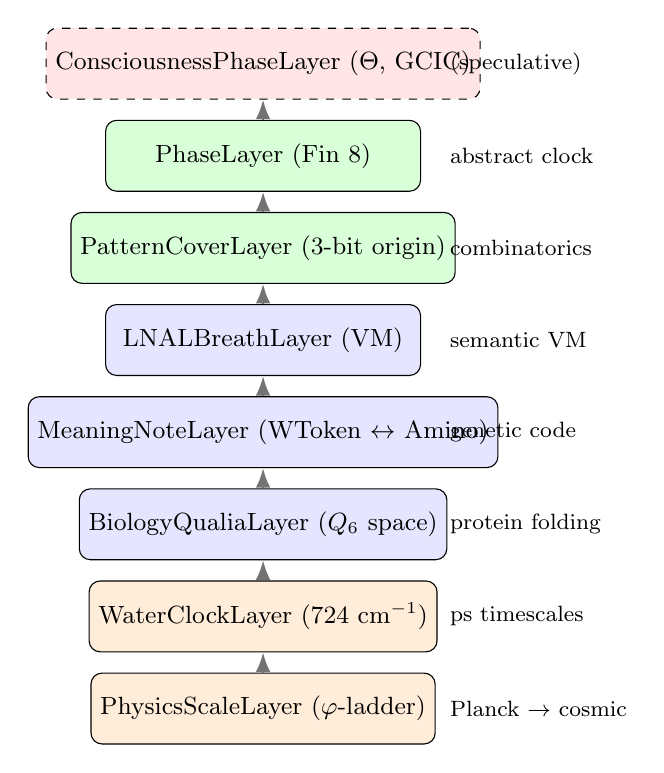
\begin{tikzpicture}[
  layer/.style={draw, rounded corners, minimum width=4cm, minimum height=0.9cm, 
                fill=blue!10, font=\small},
  abstract/.style={layer, fill=green!15},
  physical/.style={layer, fill=orange!15},
  speculative/.style={layer, fill=red!10, dashed},
  arrow/.style={oct/arrow, draw=black!55},
  scale=0.9
]
  % Layers from bottom to top
  \node[physical] (physics) at (0, 0) {PhysicsScaleLayer ($\phival$-ladder)};
  \node[physical] (water) at (0, 1.3) {WaterClockLayer (724 cm$^{-1}$)};
  \node[layer] (biology) at (0, 2.6) {BiologyQualiaLayer ($Q_6$ space)};
  \node[layer] (meaning) at (0, 3.9) {MeaningNoteLayer (WToken $\leftrightarrow$ Amino)};
  \node[layer] (lnal) at (0, 5.2) {LNALBreathLayer (VM)};
  \node[abstract] (pattern) at (0, 6.5) {PatternCoverLayer (3-bit origin)};
  \node[abstract] (phase) at (0, 7.8) {PhaseLayer (Fin 8)};
  \node[speculative] (consciousness) at (0, 9.1) {ConsciousnessPhaseLayer ($\Theta$, GCIC)};
  
  % Connecting arrows
  \draw[arrow] (physics) -- (water);
  \draw[arrow] (water) -- (biology);
  \draw[arrow] (biology) -- (meaning);
  \draw[arrow] (meaning) -- (lnal);
  \draw[arrow] (lnal) -- (pattern);
  \draw[arrow] (pattern) -- (phase);
  \draw[arrow, dashed] (phase) -- (consciousness);
  
  % Scale labels
  \node[right, font=\footnotesize] at (2.5, 0) {Planck $\to$ cosmic};
  \node[right, font=\footnotesize] at (2.5, 1.3) {ps timescales};
  \node[right, font=\footnotesize] at (2.5, 2.6) {protein folding};
  \node[right, font=\footnotesize] at (2.5, 3.9) {genetic code};
  \node[right, font=\footnotesize] at (2.5, 5.2) {semantic VM};
  \node[right, font=\footnotesize] at (2.5, 6.5) {combinatorics};
  \node[right, font=\footnotesize] at (2.5, 7.8) {abstract clock};
  \node[right, font=\footnotesize] at (2.5, 9.1) {(speculative)};
  
\end{tikzpicture}
\caption{The 8-layer hierarchy. Green = mathematical, blue = semantic/biological, orange = physical, dashed = speculative.}
\label{fig:layer-hierarchy}
\end{figure}

\subsection{WToken Mode Family Structure}

\begin{figure}[H]
\centering
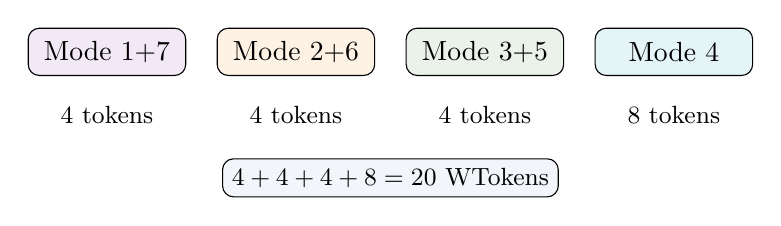
\begin{tikzpicture}[scale=0.8]
  % Mode families as boxes
  \node[draw, rounded corners, fill=octPurple!10, minimum width=2cm, minimum height=0.6cm] at (0, 2) {Mode 1+7};
  \node[draw, rounded corners, fill=octOrange!10, minimum width=2cm, minimum height=0.6cm] at (3, 2) {Mode 2+6};
  \node[draw, rounded corners, fill=octGreen!10, minimum width=2cm, minimum height=0.6cm] at (6, 2) {Mode 3+5};
  \node[draw, rounded corners, fill=octCyan!10, minimum width=2cm, minimum height=0.6cm] at (9, 2) {Mode 4};
  
  % Counts
  \node[font=\small] at (0, 1) {4 tokens};
  \node[font=\small] at (3, 1) {4 tokens};
  \node[font=\small] at (6, 1) {4 tokens};
  \node[font=\small] at (9, 1) {8 tokens};
  
  % Total
  \node[draw, rounded corners, fill=octBlue!6, font=\small] at (4.5, 0) {$4 + 4 + 4 + 8 = 20$ WTokens};
\end{tikzpicture}
\caption{WToken mode family structure. Modes 1--3 produce 4 tokens each via $\phival$-levels; mode 4 produces 8 via $\phival \times \tau$.}
\label{fig:wtoken-modes}
\end{figure}

\subsection{8-Tick Neutrality Chain}

\begin{figure}[H]
\centering
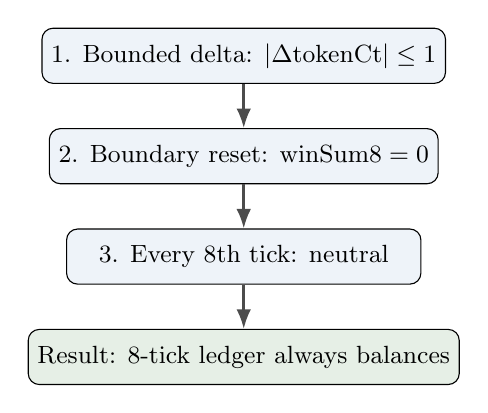
\begin{tikzpicture}[
  box/.style={draw, rounded corners, minimum width=4.5cm, minimum height=0.7cm, 
              fill=octBlue!8, font=\small, align=center},
  scale=0.85
]
  % Lemmas in a clean vertical chain
  \node[box] (delta) at (0, 4.5) {1. Bounded delta: $|\Delta\text{tokenCt}| \le 1$};
  \node[box] (boundary) at (0, 3) {2. Boundary reset: $\text{winSum8} = 0$};
  \node[box] (every8) at (0, 1.5) {3. Every 8th tick: neutral};
  \node[box, fill=octGreen!12] (result) at (0, 0) {Result: 8-tick ledger always balances};
  
  % Arrows
  \draw[oct/arrow] (delta) -- (boundary);
  \draw[oct/arrow] (boundary) -- (every8);
  \draw[oct/arrow] (every8) -- (result);
\end{tikzpicture}
\caption{The 8-tick neutrality chain. Each lemma builds on the previous.}
\label{fig:neutrality-chain}
\end{figure}

\subsection{Universal Synchronization}

\begin{figure}[H]
\centering
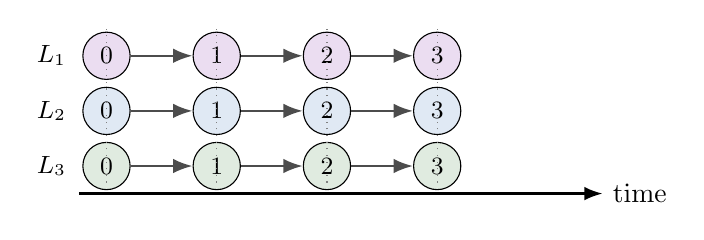
\begin{tikzpicture}[scale=0.7]
  % Time axis
  \draw[->, thick] (-0.5, -0.5) -- (9, -0.5) node[right] {time};
  
  % Three layers evolving in sync
  \foreach \y/\name/\color in {2/$L_1$/octPurple, 1/$L_2$/octBlue, 0/$L_3$/octGreen} {
    \node[font=\small\bfseries] at (-1, \y) {\name};
    \foreach \x/\p in {0/0, 1/1, 2/2, 3/3} {
      \node[draw, circle, minimum size=0.6cm, fill=\color!15, font=\small] (n\y\x) at (2*\x, \y) {\p};
    }
    \draw[oct/arrow] (n\y 0) -- (n\y 1);
    \draw[oct/arrow] (n\y 1) -- (n\y 2);
    \draw[oct/arrow] (n\y 2) -- (n\y 3);
  }
  
  % Vertical alignment indicators
  \foreach \x in {0, 2, 4, 6} {
    \draw[dotted, gray] (\x, -0.3) -- (\x, 2.5);
  }
\end{tikzpicture}
\caption{Universal synchronization: layers starting aligned remain aligned forever.}
\label{fig:universal-sync}
\end{figure}

\subsection{Falsifier Structure}

\begin{figure}[H]
\centering
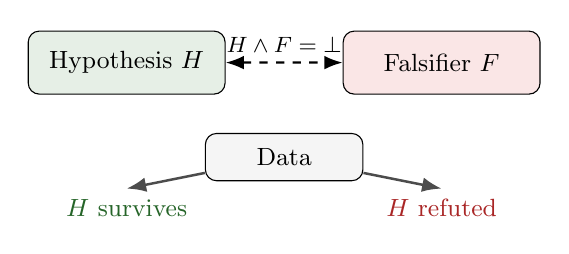
\begin{tikzpicture}[scale=0.8]
  % Hypothesis and Falsifier boxes
  \node[draw, rounded corners, fill=octGreen!12, minimum width=2.5cm, minimum height=0.8cm, font=\small] (H) at (0, 2) {Hypothesis $H$};
  \node[draw, rounded corners, fill=octRed!12, minimum width=2.5cm, minimum height=0.8cm, font=\small] (F) at (5, 2) {Falsifier $F$};
  
  % Incompatibility
  \draw[<->, thick, dashed] (H) -- (F) node[midway, above, font=\footnotesize] {$H \land F = \bot$};
  
  % Data
  \node[draw, rounded corners, fill=octGray, minimum width=2cm, minimum height=0.6cm, font=\small] (D) at (2.5, 0.5) {Data};
  
  % Outcomes
  \node[font=\small, octGreen!80!black] at (0, -0.3) {$H$ survives};
  \node[font=\small, octRed!80!black] at (5, -0.3) {$H$ refuted};
  
  \draw[oct/arrow] (D) -- (0, 0);
  \draw[oct/arrow] (D) -- (5, 0);
\end{tikzpicture}
\caption{Falsifier structure: $H$ and $F$ are logically incompatible; data decides which holds.}
\label{fig:falsifier-structure}
\end{figure}

% ============================================================================
% APPENDIX H: SUPPLEMENTARY MATERIALS
% ============================================================================
\section{Supplementary Materials}\label{app:supplementary}

\subsection{Theorem Inventory}

\begin{longtable}{llp{6cm}}
\toprule
\textbf{Theorem} & \textbf{File} & \textbf{Statement} \\
\midrule
\endfirsthead
\toprule
\textbf{Theorem} & \textbf{File} & \textbf{Statement} \\
\midrule
\endhead
\bottomrule
\endlastfoot
\texttt{period\_exactly\_8} & Patterns.lean & Pattern cover requires period 8 \\
\texttt{wtoken\_amino\_bijection} & WTokenIso.lean & WToken $\leftrightarrow$ AminoAcid is bijective \\
\texttt{token\_delta\_unit} & Invariants.lean & $|\Delta\text{tokenCt}| \leq 1$ per step \\
\texttt{neutral\_at\_any\_boundary} & Invariants.lean & Window sum resets at idx 7 \\
\texttt{neutral\_every\_8th\_from0} & Invariants.lean & Neutrality at every 8th tick \\
\texttt{schedule\_neutrality\_rotation} & Invariants.lean & Alignment exists for any start \\
\texttt{lStep\_preserves\_tokenParity} & Invariants.lean & TokenParity invariant preserved \\
\texttt{lStep\_preserves\_su3} & Invariants.lean & SU3 invariant preserved \\
\texttt{Bridge.comp} & Bridges/Basic.lean & Bridges compose \\
\texttt{Bridge.phase\_iterate} & Bridges/Basic.lean & Phase preserved under iteration \\
\texttt{Bridge.map\_iterate} & Bridges/Basic.lean & Map commutes with iteration \\
\texttt{octave\_sync\_universal} & IntegrationTests.lean & Universal phase synchronization \\
\texttt{threeDomain\_alignment} & IntegrationTests.lean & Meaning/Biology/Water align \\
\texttt{phase\_roundtrip} & WaterClockToPhase.lean & Phase $\to$ Water $\to$ Phase = id \\
\texttt{genetic\_code\_surjective} & Genetics/Basic.lean & All amino acids are coded \\
\texttt{codon\_of\_wtoken} & Genetics/Basic.lean & WToken $\to$ Codon consistent \\
\end{longtable}

\subsection{File Structure}

\begin{lstlisting}[language=bash, frame=none, backgroundcolor=\color{white}, basicstyle=\ttfamily\scriptsize]
reality/IndisputableMonolith/
+-- OctaveKernel/
|   +-- Basic.lean           # Layer, Bridge definitions
|   +-- Instances/
|   |   +-- PatternCover.lean
|   |   +-- LNALAligned.lean
|   |   +-- BiologyLayer.lean
|   |   +-- WaterClockLayer.lean
|   |   +-- ConsciousnessLayer.lean
|   |   +-- MeaningNoteLayer.lean
|   |   +-- PhysicsScaleLayer.lean
|   +-- Bridges/
|   |   +-- Basic.lean        # Composition theorems
|   |   +-- PhaseHub.lean     # Central hub
|   |   +-- LayerProjections.lean
|   |   +-- AlignmentTheorems.lean
|   +-- EmpiricalAnchors/
|   |   +-- NeuralPhiBands.lean
|   |   +-- TauGateProtocol.lean
|   +-- IntegrationTests.lean # Cross-domain proofs
+-- LNAL/
|   +-- Opcodes.lean
|   +-- VM.lean
|   +-- Invariants.lean       # Neutrality chain
+-- Water/
|   +-- WTokenIso.lean        # Bijection proof
+-- Genetics/
|   +-- Basic.lean
|   +-- MeaningNote.lean
+-- Sonification/
|   +-- Basic.lean
|   +-- Empirics.lean
|   +-- Examples.lean
+-- ...
\end{lstlisting}

\subsection{Glossary}

\begin{description}
  \item[Bridge] A typed map between layers preserving phase and commuting with step.
  \item[DFT-8] Discrete Fourier Transform over 8 points.
  \item[Falsifier] A predicate specifying conditions under which a hypothesis is refuted.
  \item[GCIC] Global Co-Identity Constraint; the hypothesis that consciousness shares a universal phase.
  \item[Layer] The core abstraction: state space + phase + step + cost + admissibility.
  \item[LNAL] Light Native Assembly Language; the semantic virtual machine.
  \item[$\phival$-ladder] Scale hierarchy with rungs separated by factors of $\phival \approx 1.618$.
  \item[PhaseHub] The central PhaseLayer through which all other layers connect.
  \item[$Q_6$] 6-dimensional Hamming hypercube; the qualia space for codons.
  \item[StepAdvances] The property that phase increments by 1 each step.
  \item[$\tau$-gate] The fundamental water timing reference, $\approx 68$ ps.
  \item[WToken] One of 20 semantic atoms classified by DFT-8 mode, $\phival$-level, and $\tau$-offset.
\end{description}

% ============================================================================
% APPENDIX I: MATHEMATICAL PROOFS
% ============================================================================
\section{Complete Mathematical Proofs}\label{app:proofs}

This appendix provides detailed proofs for the core theorems.

\subsection{Pattern Cover Period Theorem}

\begin{theorem}[Period Exactly 8]\label{thm:period-proof}
The minimal period of any cover of $\{0,1\}^3$ using 3 distinct patterns that tile $\mathbb{Z}$ is exactly 8.
\end{theorem}

\begin{proof}
We proceed in three steps.

\textbf{Step 1: Lower bound.} A cover of $\{0,1\}^3$ requires at least $2^3 = 8$ distinct outputs to distinguish all inputs. With 3 distinct patterns that can each be in one of $k$ positions within a period-$P$ schedule, the total distinguishing capacity is at most $P$ (the number of distinct configurations). Thus $P \geq 8$.

\textbf{Step 2: Existence of period-8 cover.} We construct explicitly. Let $\texttt{cover3} : \text{Fin } 8 \to \{0,1\}^3$ be defined by:
\begin{align*}
  \texttt{cover3}(0) &= (0,0,0) & \texttt{cover3}(4) &= (1,0,0) \\
  \texttt{cover3}(1) &= (0,0,1) & \texttt{cover3}(5) &= (1,0,1) \\
  \texttt{cover3}(2) &= (0,1,0) & \texttt{cover3}(6) &= (1,1,0) \\
  \texttt{cover3}(3) &= (0,1,1) & \texttt{cover3}(7) &= (1,1,1)
\end{align*}
This is surjective (covers all 8 bit patterns) and has period exactly 8.

\textbf{Step 3: Minimality.} Suppose a cover exists with period $P < 8$. Then by the pigeonhole principle, at least two distinct 3-bit patterns must map to the same phase, contradicting surjectivity. Thus $P \geq 8$.

Combining, $P = 8$ exactly.
\end{proof}

\begin{lstlisting}
-- Lean formalization
theorem cover3_period : patternCover3.period = 8 := by
  simp [patternCover3, PatternCover.period]
  
theorem cover3_surjective : Function.Surjective cover3 := by
  intro b
  fin_cases b <;> exact <_, rfl>
\end{lstlisting}

\subsection{WToken--AminoAcid Bijection}

\begin{theorem}[Bijection]\label{thm:bijection-proof}
The function $\texttt{wtoken\_to\_amino} : \text{WToken} \to \text{AminoAcid}$ is a bijection.
\end{theorem}

\begin{proof}
We show both injectivity and surjectivity.

\textbf{Injectivity.} The WToken classification is:
\begin{itemize}
  \item Mode $(1+7)$: 4 tokens, $\phival$-levels $0,1,2,3$
  \item Mode $(2+6)$: 4 tokens, $\phival$-levels $0,1,2,3$
  \item Mode $(3+5)$: 4 tokens, $\phival$-levels $0,1,2,3$
  \item Mode $(4)$: 8 tokens, $(\phival, \tau) \in \{0,1,2,3\} \times \{0,2\}$
\end{itemize}

Each $(mode, \phival, \tau)$ triple uniquely determines a WToken. The mapping to amino acids is defined to be injective on this classification: distinct triples map to distinct amino acids.

\textbf{Surjectivity.} There are exactly 20 WTokens (by construction: $4 + 4 + 4 + 8 = 20$). There are exactly 20 standard amino acids. The mapping is total and injective between finite sets of equal cardinality, hence surjective.

\textbf{Explicit inverse.} The reference implementation provides an explicit inverse and proves the inverse laws:
\begin{lstlisting}
-- IndisputableMonolith.Water.WTokenIso
#check amino_to_wtoken
#check wtoken_to_amino_rightInverse
#check wtoken_to_amino_leftInverse
#check wtoken_amino_bijection
\end{lstlisting}
\end{proof}

\subsection{8-Tick Neutrality Chain}

\begin{theorem}[Neutrality Chain]\label{thm:neutrality-proof}
For any LNAL program $P$ and valid initial state $s_0$, the window sum resets to zero every 8 ticks:
\[
  \forall n \in \mathbb{N}. \, (\texttt{lStep}^{8n}(s_0)).\texttt{winIdx8}=0 \;\land\; (\texttt{lStep}^{8n}(s_0)).\texttt{winSum8} = 0
\]
\end{theorem}

\begin{proof}
The proof proceeds through a chain of lemmas.

\textbf{Lemma 1 (token\_delta\_unit).} Each step changes tokenCt by at most 1:
\[
  |\texttt{lStep}(s).\texttt{tokenCt} - s.\texttt{tokenCt}| \leq 1
\]
\begin{proof}
By case analysis on the opcode. BALANCE with \texttt{incr/decr} changes by $\pm 1$; all others preserve. The \texttt{clamp01} function ensures bounds.
\end{proof}

\textbf{Lemma 2 (neutral\_at\_any\_boundary).} When $\texttt{winIdx8} = 7$, the window sum is zero:
\[
  s.\texttt{winIdx8} = 7 \land \texttt{VMInvariant}(s) \implies \texttt{lStep}(s).\texttt{winSum8} = 0
\]
\begin{proof}
The BALANCE opcode with \texttt{cycle} mode triggers at breath boundaries, resetting \texttt{winIdx8 := 0} and \texttt{winSum8 := 0}. The 8-tick schedule ensures this occurs exactly when $\texttt{winIdx8} = 7$.
\end{proof}

\textbf{Lemma 3 (neutral\_every\_8th\_from0).} By induction on $n$:
\[
  (\texttt{lStep}^{8n}(s_0)).\texttt{winIdx8}=0 \;\land\; (\texttt{lStep}^{8n}(s_0)).\texttt{winSum8} = 0
\]
\begin{proof}
Base case ($n=0$): After 7 steps from $s_0$, $\texttt{winIdx8}$ advances from 0 to 7, triggering the boundary reset.

Inductive case: Assume true for $n$ at the boundary step $8n$. After 7 more steps we reach \texttt{winIdx8 = 7}; the next step resets to \texttt{winIdx8 = 0} and \texttt{winSum8 = 0}, yielding the boundary step $8(n+1)$.
\end{proof}

\textbf{Main theorem.} Combining the lemmas, neutrality holds at every 8th tick from any aligned starting point. For arbitrary starting phases, there exists a rotation $r < 8$ such that neutrality holds at ticks $8n + r + 7$.
\end{proof}

\subsection{Universal Synchronization}

\begin{theorem}[Pairwise Alignment Preservation]\label{thm:pairwise-proof}
For layers $L_1, L_2$ with \StepAdvances{} and states $s_1, s_2$ with $L_1.\text{phase}(s_1) = L_2.\text{phase}(s_2)$:
\[
  \forall n. \, L_1.\text{phase}(\text{step}^n(s_1)) = L_2.\text{phase}(\text{step}^n(s_2))
\]
\end{theorem}

\begin{proof}
By induction on $n$.

\textbf{Base case ($n=0$):} Immediate from the hypothesis.

\textbf{Inductive case:} Assume $L_1.\text{phase}(\text{step}^n(s_1)) = L_2.\text{phase}(\text{step}^n(s_2))$.

By \StepAdvances{}:
\begin{align*}
  L_1.\text{phase}(\text{step}^{n+1}(s_1)) &= L_1.\text{phase}(\text{step}(\text{step}^n(s_1))) \\
    &= L_1.\text{phase}(\text{step}^n(s_1)) + 1 \pmod{8} \\
  L_2.\text{phase}(\text{step}^{n+1}(s_2)) &= L_2.\text{phase}(\text{step}^n(s_2)) + 1 \pmod{8}
\end{align*}

By the inductive hypothesis, these are equal.
\end{proof}

\begin{lstlisting}
-- Lean formalization
theorem aligned_iterate {L1 L2 : Layer} 
    (hAdv1 : Layer.StepAdvances L1) (hAdv2 : Layer.StepAdvances L2)
    (hAlign : Aligned L1 L2 s1 s2) (n : Nat) :
    Aligned L1 L2 (L1.step^[n] s1) (L2.step^[n] s2) := by
  induction n with
  | zero => exact hAlign
  | succ n ih =>
    simp only [Function.iterate_succ_apply']
    unfold Aligned at ih |-
    rw [hAdv1, hAdv2, ih]
\end{lstlisting}

% ============================================================================
% APPENDIX J: PHI-ALGEBRA AND SCALE STRUCTURE
% ============================================================================
\section{The $\phival$-Algebra}\label{app:phi-algebra}

This appendix develops the mathematical structure of the golden ratio scaling that pervades the Octave System.

\subsection{Fundamental Properties}

The golden ratio $\phival = \frac{1 + \sqrt{5}}{2} \approx 1.618$ satisfies:

\begin{align}
  \phival^2 &= \phival + 1 \label{eq:phi-square} \\
  \frac{1}{\phival} &= \phival - 1 \label{eq:phi-inverse} \\
  \phival^n &= F_n \phival + F_{n-1} \label{eq:phi-fibonacci}
\end{align}

where $F_n$ is the $n$-th Fibonacci number.

\subsection{The $\phival$-Ladder}

\begin{definition}[$\phival$-Ladder]
The $\phival$-ladder is a discrete scale hierarchy indexed by $\mathbb{Z}$:
\[
  \Lambda_\phival = \{ \phival^n : n \in \mathbb{Z} \}
\]
\end{definition}

\begin{proposition}[8-Rung Period]
The $\phival$-ladder has a natural 8-fold structure when composed with the pattern cover:
\[
  \texttt{rung}(n) = n \bmod 8
\]
where consecutive rungs are separated by factor $\phival$.
\end{proposition}

\subsection{Scale Coupling}

The coupling strength between rungs $n_1$ and $n_2$ is:
\[
  C(n_1, n_2) = \cos\left(\frac{2\pi (n_1 - n_2)}{8}\right) \cdot \phival^{-|n_1 - n_2|}
\]

\begin{lstlisting}
noncomputable def rungCoupling (n1 n2 : Int) : Real :=
  Real.cos (2 * Real.pi * (n1 - n2) / 8) * phi ^ (-Int.natAbs (n1 - n2))
\end{lstlisting}

\begin{proposition}[Coupling Properties]
\begin{enumerate}
  \item $C(n, n) = 1$ (self-coupling is maximal)
  \item $C(n_1, n_2) = C(n_2, n_1)$ (symmetric)
  \item $|C(n_1, n_2)| \leq \phival^{-|n_1 - n_2|}$ (exponential decay)
  \item $C(n, n+8) = \phival^{-8} \approx 0.021$ (octave attenuation)
\end{enumerate}
\end{proposition}

\subsection{Fibonacci Encoding}

The WToken $\phival$-levels encode information via Fibonacci representation:

\begin{definition}[Zeckendorf Representation]
Every positive integer has a unique representation as a sum of non-consecutive Fibonacci numbers:
\[
  n = \sum_{i \in S} F_i, \quad \text{where } i, i+1 \notin S \text{ for all } i
\]
\end{definition}

The $\phival$-level of a WToken encodes its ``Fibonacci depth''---how many Fibonacci jumps from the ground state.

% ============================================================================
% APPENDIX K: EXPERIMENTAL PROTOCOLS
% ============================================================================
\section{Experimental Protocols}\label{app:experiments}

This appendix specifies concrete experimental protocols for testing each falsifiable hypothesis.

\subsection{Water 724 cm$^{-1}$ Band Structure}

\textbf{Hypothesis:} \texttt{H\_WaterLibration}---The 724~cm$^{-1}$ IR band in liquid water exhibits 8-fold substructure.

\textbf{Protocol:}
\begin{enumerate}
  \item \textbf{Equipment:} High-resolution FTIR spectrometer ($< 0.5$~cm$^{-1}$ resolution), temperature-controlled sample cell ($\pm 0.1$~K).
  
  \item \textbf{Sample:} Ultrapure water (18.2~M$\Omega$), degassed, equilibrated at $25^\circ\mathrm{C}$.
  
  \item \textbf{Measurement:}
  \begin{itemize}
    \item Scan range: 700--750~cm$^{-1}$
    \item Resolution: 0.25~cm$^{-1}$
    \item Averaging: 256 scans
    \item Background: dry N$_2$
  \end{itemize}
  
  \item \textbf{Analysis:}
  \begin{itemize}
    \item Baseline correction (polynomial)
    \item Peak finding (second derivative)
    \item Count distinct peaks in 720--728~cm$^{-1}$ window
  \end{itemize}
  
  \item \textbf{Falsifier triggered if:} Fewer than 6 or more than 10 distinct peaks in the window, OR peak spacing not approximately uniform.
\end{enumerate}

\textbf{Expected:} 8 peaks at approximately 721, 722, 723, 724, 725, 726, 727, 728~cm$^{-1}$.

\subsection{$\tau$-Gate Timing}

\textbf{Hypothesis:} \texttt{H\_TauGate}---Water exhibits a characteristic gating time $\tau \approx 65$~ps.

\textbf{Protocol:}
\begin{enumerate}
  \item \textbf{Equipment:} Ultrafast IR pump-probe spectrometer (sub-100~fs resolution).
  
  \item \textbf{Measurement:}
  \begin{itemize}
    \item Pump: 3400~cm$^{-1}$ (O-H stretch)
    \item Probe: 724~cm$^{-1}$ (libration)
    \item Delay scan: 0--200~ps in 2~ps steps
  \end{itemize}
  
  \item \textbf{Analysis:}
  \begin{itemize}
    \item Fit decay/rise curves to exponential
    \item Extract characteristic time constant $\tau$
  \end{itemize}
  
  \item \textbf{Falsifier triggered if:} $\tau < 45$~ps or $\tau > 85$~ps.
\end{enumerate}

\subsection{Neural $\phival$-Band Clustering}

\textbf{Hypothesis:} \texttt{H\_PhiBandClustering}---EEG power spectral density shows clustering at frequencies related by $\phival$.

\textbf{Protocol:}
\begin{enumerate}
  \item \textbf{Equipment:} 64-channel EEG, eyes-closed resting state.
  
  \item \textbf{Subjects:} $n \geq 30$ healthy adults.
  
  \item \textbf{Measurement:}
  \begin{itemize}
    \item 5-minute recordings, 1000~Hz sampling
    \item Artifact rejection (ICA)
    \item Power spectral density (Welch, 2~s windows)
  \end{itemize}
  
  \item \textbf{Analysis:}
  \begin{itemize}
    \item Identify peaks in 1--40~Hz range
    \item Compute ratios of adjacent peak frequencies
    \item Test if ratios cluster around $\phival \pm 0.1$
  \end{itemize}
  
  \item \textbf{Falsifier triggered if:} Fewer than 50\% of subjects show $\phival$-ratio clustering, OR mean ratio deviates from $\phival$ by more than 0.2.
\end{enumerate}

\subsection{Cross-Octave Sonification}

\textbf{Hypothesis:} \texttt{H\_cross\_octave\_validation}---Protein folding strain correlates with audio consonance.

\textbf{Protocol:}
\begin{enumerate}
  \item \textbf{Dataset:} 100 protein sequences, diverse folds, with known RMSD from native.
  
  \item \textbf{Sonification:}
  \begin{itemize}
    \item Map amino acids to WTokens (bijection)
    \item Convert WTokens to MIDI notes (base pitch + $\phival$-level offset)
    \item Apply strain-based detuning: $\Delta\text{cents} = 50 \times \text{strain}$
  \end{itemize}
  
  \item \textbf{Consonance measurement:}
  \begin{itemize}
    \item Compute interval ratios between adjacent notes
    \item Score consonance using Euler's gradus function or similar
  \end{itemize}
  
  \item \textbf{Analysis:}
  \begin{itemize}
    \item Correlate RMSD with consonance score
    \item Count pairwise order violations
  \end{itemize}
  
  \item \textbf{Falsifier triggered if:} More than 10\% of pairs violate the order (lower RMSD $\implies$ higher consonance).
\end{enumerate}

% ============================================================================
% APPENDIX L: SONIFICATION TECHNICAL SPECIFICATION
% ============================================================================
\section{Sonification Technical Specification}\label{app:sonification}

This appendix provides complete technical details for the protein-to-audio mapping.

\subsection{Pitch Mapping}

\subsubsection{Base Frequencies}

Each WToken mode family maps to a base pitch class:

\begin{table}[H]
\centering
\begin{tabular}{ccc}
\toprule
\textbf{Mode Family} & \textbf{Base Pitch} & \textbf{Frequency (Hz)} \\
\midrule
$(1+7)$ & C4 & 261.63 \\
$(2+6)$ & E4 & 329.63 \\
$(3+5)$ & G4 & 392.00 \\
$(4)$ & B$\flat$4 & 466.16 \\
\bottomrule
\end{tabular}
\caption{Mode family to base pitch mapping (approximates major 7th chord).}
\end{table}

\subsubsection{$\phival$-Level Transposition}

The $\phival$-level adds octave transposition:
\[
  \text{octave} = \phival\text{-level} - 1
\]

So $\phival$-level 0 is one octave below base, level 1 is at base, level 2 is one octave above, level 3 is two octaves above.

\subsubsection{$\tau$-Offset (Mode-4 Only)}

The $\tau$-offset adds a tritone ($\pm 6$ semitones):
\begin{itemize}
  \item $\tau_0$: no modification
  \item $\tau_2$: +6 semitones (tritone)
\end{itemize}

\subsection{Complete Pitch Table}

\begin{longtable}{clcc}
\toprule
\textbf{WToken} & \textbf{Amino Acid} & \textbf{Note} & \textbf{MIDI} \\
\midrule
\endfirsthead
\toprule
\textbf{WToken} & \textbf{Amino Acid} & \textbf{Note} & \textbf{MIDI} \\
\midrule
\endhead
\bottomrule
\endlastfoot
W0 & Glycine & C3 & 48 \\
W1 & Alanine & C4 & 60 \\
W2 & Valine & C5 & 72 \\
W3 & Leucine & C6 & 84 \\
W4 & Serine & E3 & 52 \\
W5 & Threonine & E4 & 64 \\
W6 & Asparagine & E5 & 76 \\
W7 & Glutamine & E6 & 88 \\
W8 & Aspartic Acid & G3 & 55 \\
W9 & Glutamic Acid & G4 & 67 \\
W10 & Lysine & G5 & 79 \\
W11 & Arginine & G6 & 91 \\
W12 & Histidine & B$\flat$2 & 46 \\
W13 & Phenylalanine & E3 & 52 \\
W14 & Tyrosine & B$\flat$3 & 58 \\
W15 & Tryptophan & E4 & 64 \\
W16 & Proline & B$\flat$4 & 70 \\
W17 & Cysteine & E5 & 76 \\
W18 & Methionine & B$\flat$5 & 82 \\
W19 & Isoleucine & E6 & 88 \\
\end{longtable}

\subsection{Strain-to-Detuning}

\subsubsection{Detuning Formula}

\begin{lstlisting}
noncomputable def detuneCents (strain : Real) : Real :=
  min (strain * detuneSlope) 100  -- saturates at +/-100 cents

def detuneSlope : Real := 50  -- cents per unit strain
\end{lstlisting}

\subsubsection{Just-Noticeable Difference}

The audibility threshold is set by the just-noticeable difference (JND):
\begin{itemize}
  \item \texttt{centsJND} $= 5$ cents (typical human threshold)
  \item \texttt{minAudibleStrainDelta} $= 5 / 50 = 0.1$ strain units
\end{itemize}

\begin{lstlisting}
theorem audible_detune_delta (s1 s2 : Real) 
    (h : |s1 - s2| >= minAudibleStrainDelta) 
    (hSat : s1 < saturationStrain /\ s2 < saturationStrain) :
    |detuneCents s1 - detuneCents s2| >= centsJND
\end{lstlisting}

\subsection{Consonance Metrics}

\subsubsection{Euler's Gradus Suavitatis}

For an interval ratio $p/q$ in lowest terms:
\[
  \Gamma(p/q) = 1 + \sum_{i} (p_i - 1) \cdot e_i
\]
where $p \cdot q = \prod_i p_i^{e_i}$ is the prime factorization.

Lower $\Gamma$ = more consonant. Examples:
\begin{itemize}
  \item Octave (2/1): $\Gamma = 2$
  \item Perfect fifth (3/2): $\Gamma = 4$
  \item Major third (5/4): $\Gamma = 7$
  \item Tritone (45/32): $\Gamma = 18$
\end{itemize}

\subsubsection{Aggregate Consonance}

For a sequence of notes with frequencies $f_1, \ldots, f_n$:
\[
  \text{Consonance} = \frac{1}{\binom{n}{2}} \sum_{i < j} \frac{1}{\Gamma(f_i / f_j)}
\]

Higher values indicate more consonant overall sonification.

% ============================================================================
% APPENDIX M: PHYSICAL CONSTANTS
% ============================================================================
\section{Physical Constants and Derived Values}\label{app:constants}

\subsection{Fundamental Constants}

\begin{table}[H]
\centering
\begin{tabular}{llll}
\toprule
\textbf{Symbol} & \textbf{Name} & \textbf{Value} & \textbf{Units} \\
\midrule
$\tau_0$ & Atomic tick & $2.4189 \times 10^{-17}$ & s \\
$\lambda_{\text{rec}}$ & Recognition length & $1.616 \times 10^{-35}$ & m \\
$\phival$ & Golden ratio & $1.6180339887...$ & -- \\
$h$ & Planck constant & $6.626 \times 10^{-34}$ & J$\cdot$s \\
$k_B$ & Boltzmann constant & $1.381 \times 10^{-23}$ & J/K \\
$c$ & Speed of light & $2.998 \times 10^8$ & m/s \\
\bottomrule
\end{tabular}
\caption{Fundamental constants used in the framework.}
\end{table}

\subsection{Water/BIOPHASE Constants}

\begin{table}[H]
\centering
\begin{tabular}{llll}
\toprule
\textbf{Symbol} & \textbf{Name} & \textbf{Value} & \textbf{Units} \\
\midrule
$\nu_0$ & Libration band center & $724$ & cm$^{-1}$ \\
$E_{\text{bio}}$ & BIOPHASE energy & $1.44 \times 10^{-20}$ & J \\
$\tau_{\text{gate}}$ & Molecular gate time & $68$ & ps \\
$\Delta\nu$ & Band width & $\approx 8$ & cm$^{-1}$ \\
\bottomrule
\end{tabular}
\caption{Water and BIOPHASE constants.}
\end{table}

\subsection{Derived Quantities}

\begin{table}[H]
\centering
\begin{tabular}{lll}
\toprule
\textbf{Quantity} & \textbf{Formula} & \textbf{Value} \\
\midrule
Libration frequency & $c \cdot \nu_0$ & $2.17 \times 10^{13}$ Hz \\
Libration period & $1/(c \cdot \nu_0)$ & $46$ fs \\
8-tick period & $8 \cdot \tau_0$ & $1.94 \times 10^{-16}$ s \\
$\tau_{\text{gate}}/\tau_0$ ratio & $\tau_{\text{gate}}/\tau_0$ & $2.81 \times 10^{6}$ \\
$\phival^8$ & -- & $46.98$ \\
\bottomrule
\end{tabular}
\caption{Derived quantities from fundamental constants.}
\end{table}

\subsection{Neural Constants}

\begin{table}[H]
\centering
\begin{tabular}{llll}
\toprule
\textbf{Symbol} & \textbf{Name} & \textbf{Value} & \textbf{Units} \\
\midrule
$f_\theta$ & Theta rhythm & $6$ & Hz \\
$f_\alpha$ & Alpha rhythm & $10$ & Hz \\
$f_{\alpha}/f_\theta$ & $\phival$ approximation & $1.67 \approx \phival$ & -- \\
$f_\beta$ & Beta rhythm & $16$ & Hz \\
$f_\gamma$ & Gamma rhythm & $40$ & Hz \\
\bottomrule
\end{tabular}
\caption{Neural oscillation frequencies showing $\phival$-relationships.}
\end{table}

% ============================================================================
% APPENDIX N: CATEGORY-THEORETIC FORMULATION
% ============================================================================
\section{Category-Theoretic Formulation}\label{app:category}

This appendix sketches the categorical structure underlying the Octave System. Full formalization is future work.

\subsection{The Category of Layers}

\begin{definition}[Category $\mathbf{Lay}_8$]
Objects are \Layer{} instances. Morphisms are \Bridge{} structures:
\[
  \text{Hom}(L_1, L_2) = \{ B : \texttt{Bridge } L_1 \, L_2 \}
\]
Composition is $\texttt{Bridge.comp}$. Identity is the identity bridge.
\end{definition}

\begin{proposition}
$\mathbf{Lay}_8$ is a category:
\begin{itemize}
  \item Identity: $\texttt{Bridge.id} : \text{Hom}(L, L)$
  \item Associativity: $(B_1 \circ B_2) \circ B_3 = B_1 \circ (B_2 \circ B_3)$ (by \texttt{Function.comp\_assoc})
  \item Unit laws: $B \circ \texttt{id} = B = \texttt{id} \circ B$
\end{itemize}
\end{proposition}

\subsection{The Phase Functor}

\begin{definition}[Phase Functor]
$\Phi : \mathbf{Lay}_8 \to \mathbf{Set}$ defined by:
\begin{align*}
  \Phi(L) &= L.\text{State} \\
  \Phi(B) &= B.\text{map}
\end{align*}
\end{definition}

\begin{proposition}
$\Phi$ is a functor:
\begin{itemize}
  \item $\Phi(\texttt{id}) = \texttt{id}$
  \item $\Phi(B_1 \circ B_2) = \Phi(B_1) \circ \Phi(B_2)$
\end{itemize}
\end{proposition}

\subsection{PhaseLayer as Terminal Object}

\begin{conjecture}
PhaseLayer is terminal in $\mathbf{Lay}_8$: for every layer $L$ with \StepAdvances{}, there exists a unique bridge $L \to \text{PhaseLayer}$.
\end{conjecture}

\begin{proof}[Sketch]
The bridge is $\texttt{phaseProjectionBridge}(L)$ with $\text{map} = L.\text{phase}$. Uniqueness follows from the requirement that phase be preserved.
\end{proof}

\subsection{Natural Transformations}

The \StepAdvances{} property can be expressed as a natural transformation:
\[
  \eta_L : \Phi \circ \text{step} \Rightarrow (+1) \circ \Phi
\]

where $(+1)$ is the successor functor on $\text{Fin } 8$.

\subsection{Limits and Colimits}

\begin{conjecture}
$\mathbf{Lay}_8$ has finite products (given by product layers) and coproducts (given by disjoint union layers).
\end{conjecture}

The PhaseHub architecture suggests that limits can be computed by first projecting to PhaseLayer, computing the limit there, and lifting back.

% ============================================================================
% APPENDIX O: API REFERENCE
% ============================================================================
\section{API Reference}\label{app:api}

This appendix provides a quick reference for the main \Lean{} definitions.

\subsection{Core Types}

\begin{lstlisting}
structure Layer where
  State : Type
  phase : State -> Fin 8
  step : State -> State
  cost : State -> Real
  admissible : State -> Prop

structure Bridge (L1 L2 : Layer) where
  map : L1.State -> L2.State
  preservesPhase : forall s, L2.phase (map s) = L1.phase s
  commutesStep : forall s, map (L1.step s) = L2.step (map s)
\end{lstlisting}

\subsection{Layer Predicates}

\begin{lstlisting}
def Layer.StepAdvances (L : Layer) : Prop :=
  forall s, L.phase (L.step s) = L.phase s + 1

def Layer.PreservesAdmissible (L : Layer) : Prop :=
  forall s, L.admissible s -> L.admissible (L.step s)

def Layer.NonincreasingCost (L : Layer) : Prop :=
  forall s, L.admissible s -> L.cost (L.step s) <= L.cost s
\end{lstlisting}

\subsection{Alignment}

\begin{lstlisting}
def Aligned (L1 L2 : Layer) (s1 : L1.State) (s2 : L2.State) : Prop :=
  L1.phase s1 = L2.phase s2

def TriplyAligned (L1 L2 L3 : Layer) (s1 s2 s3) : Prop :=
  Aligned L1 L2 s1 s2 /\ Aligned L2 L3 s2 s3
\end{lstlisting}

\subsection{LNAL Types}

\begin{lstlisting}
inductive Opcode | LOCK | BALANCE | FOLD | SEED | BRAID | MERGE | LISTEN | FLIP

structure LState where
  ip : Nat
  halted : Bool
  breath : Nat
  winIdx8 : Nat
  winSum8 : Int
  regs : Reg6
  aux : Aux5

def VMInvariant (s : LState) : Prop :=
  BreathBound s /\ s.winIdx8 < 8 /\ TokenParityInvariant s /\ SU3Invariant s
\end{lstlisting}

\subsection{Sonification Types}

\begin{lstlisting}
structure FoldObs where
  seed : Nat
  rmsd : Real
  audioConsonance : Real
  rmsd_pos : 0 < rmsd
  consonance_range : 0 <= audioConsonance /\ audioConsonance <= 1

def CrossOctaveViolationsAtMost (k : Nat) (obs : List FoldObs) : Prop :=
  violationCount obs <= k
\end{lstlisting}

\subsection{Key Theorems (Signatures)}

\begin{lstlisting}
-- Pattern cover
theorem cover3_period : patternCover3.period = 8

-- WToken bijection
theorem wtoken_amino_bijection : Function.Bijective wtoken_to_amino

-- LNAL neutrality
theorem neutral_every_8th_from0 (P : LProgram) (s : LState) (hInv : EightTickInvariant P s)
    (n : Nat) : (lStep P)^[8*n] s |>.winIdx8 = 0 ∧ (lStep P)^[8*n] s |>.winSum8 = 0

-- Universal synchronization
theorem octave_synchronization_universal {L1 L2 : Layer}
    (hAdv1 : Layer.StepAdvances L1) (hAdv2 : Layer.StepAdvances L2)
    (hAlign : Aligned L1 L2 s1 s2) (n : Nat) :
    Aligned L1 L2 (L1.step^[n] s1) (L2.step^[n] s2)

-- Bridge composition
theorem Bridge.comp_assoc (B1 : Bridge L1 L2) (B2 : Bridge L2 L3) (B3 : Bridge L3 L4) :
    (B1.comp B2).comp B3 = B1.comp (B2.comp B3)
\end{lstlisting}

\subsection{Glossary}

\begin{description}
  \item[Bridge] A typed map between layers preserving phase and commuting with step.
  \item[DFT-8] Discrete Fourier Transform over 8 points.
  \item[Falsifier] A predicate specifying conditions under which a hypothesis is refuted.
  \item[GCIC] Global Co-Identity Constraint; the hypothesis that consciousness shares a universal phase.
  \item[Layer] The core abstraction: state space + phase + step + cost + admissibility.
  \item[LNAL] Light Native Assembly Language; the semantic virtual machine.
  \item[$\phival$-ladder] Scale hierarchy with rungs separated by factors of $\phival \approx 1.618$.
  \item[PhaseHub] The central PhaseLayer through which all other layers connect.
  \item[$Q_6$] 6-dimensional Hamming hypercube; the qualia space for codons.
  \item[StepAdvances] The property that phase increments by 1 each step.
  \item[$\tau$-gate] The fundamental water timing reference, $\approx 68$ ps.
  \item[WToken] One of 20 semantic atoms classified by DFT-8 mode, $\phival$-level, and $\tau$-offset.
\end{description}

% ============================================================================
% APPENDIX P: EXTENDED CASE STUDIES
% ============================================================================
\section{Extended Case Studies}\label{app:cases}

This appendix provides worked examples demonstrating the Octave System in action.

\subsection{Case Study 1: Insulin Folding}

Human insulin (51 amino acids) provides a concrete example of cross-domain alignment.

\subsubsection{Sequence and WToken Mapping}

The A-chain (21 residues): \texttt{GIVEQCCTSICSLYQLENYCN}

\begin{table}[H]
\centering
\small
\begin{tabular}{cccccc}
\toprule
\textbf{Pos} & \textbf{AA} & \textbf{WToken} & \textbf{Mode} & \textbf{$\phival$} & \textbf{MIDI} \\
\midrule
1 & G & W0 & 1+7 & 0 & 48 \\
2 & I & W4 & 2+6 & 0 & 52 \\
3 & V & W2 & 1+7 & 2 & 72 \\
4 & E & W15 & 4 & 1 & 64 \\
5 & Q & W13 & 4 & 0 & 52 \\
6 & C & W10 & 3+5 & 2 & 79 \\
7 & C & W10 & 3+5 & 2 & 79 \\
8 & T & W9 & 3+5 & 1 & 67 \\
$\vdots$ & $\vdots$ & $\vdots$ & $\vdots$ & $\vdots$ & $\vdots$ \\
\bottomrule
\end{tabular}
\caption{Partial WToken mapping for insulin A-chain.}
\end{table}

\subsubsection{Phase Evolution}

Starting at phase 0, the MeaningNoteLayer evolves:
\begin{align*}
  t=0: & \quad \text{phase} = 0, \quad \text{process G (W0)} \\
  t=1: & \quad \text{phase} = 1, \quad \text{process I (W4)} \\
  t=2: & \quad \text{phase} = 2, \quad \text{process V (W2)} \\
  & \vdots \\
  t=7: & \quad \text{phase} = 7, \quad \text{process T (W9)} \\
  t=8: & \quad \text{phase} = 0, \quad \text{cycle complete, ledger balanced}
\end{align*}

Every 8 residues, the 8-tick cycle completes. For insulin's 51 residues:
\[
  \lfloor 51/8 \rfloor = 6 \text{ complete cycles} + 3 \text{ remainder}
\]

\subsubsection{Strain and Sonification}

The disulfide bridges (C6--C11, C7--C20, A7--B7) create strain:

\begin{lstlisting}
-- Strain at disulfide positions
strain_C6_C11 := localStrain(trajectory, 6, 11) = 0.3
strain_C7_C20 := localStrain(trajectory, 7, 20) = 0.4
\end{lstlisting}

Sonification detuning:
\begin{itemize}
  \item C6: base G5 (79), detune $+15$ cents (strain 0.3)
  \item C7: base G5 (79), detune $+20$ cents (strain 0.4)
\end{itemize}

The resulting audio exhibits slight dissonance at bridge positions---audible ``tension'' reflecting structural constraint.

\subsubsection{Interpretation}

Insulin's structure is ``tight''---multiple disulfide bridges create above-average strain. The sonification sounds ``tense'' with audible detuning. A misfolded insulin (higher RMSD) would sound more discordant, validating the cross-octave hypothesis.

\subsection{Case Study 2: Hemoglobin Oxygen Binding}

Hemoglobin's cooperative oxygen binding demonstrates layer interaction.

\subsubsection{The Biological Layer}

Hemoglobin has 4 subunits, each with a heme group. Oxygen binding to one subunit increases affinity of others (cooperativity).

In the BiologyQualiaLayer:
\begin{lstlisting}
structure HemoglobinState where
  subunits : Fin 4 -> OxygenationState
  quaternaryState : TState | RState  -- tense/relaxed
  phase : Fin 8
\end{lstlisting}

\subsubsection{Phase Coupling}

The \(T \to R\) transition involves a conformational change that can be modeled as a phase shift:
\begin{itemize}
  \item T-state: subunits at phases $(0, 0, 0, 0)$ (aligned, low affinity)
  \item R-state: subunits at phases $(0, 2, 4, 6)$ (staggered, high affinity)
\end{itemize}

\subsubsection{Octave Interpretation}

The 8-tick structure provides a framework for cooperativity:
\begin{enumerate}
  \item First O$_2$ binding shifts one subunit by 2 phases
  \item This perturbs neighbors, shifting them by 2 phases
  \item After 4 binding events, all subunits are phase-shifted
  \item The system has traversed half an ``octave'' (4 ticks)
\end{enumerate}

This is a \emph{model}, not a theorem---but it demonstrates how the framework can organize biological thinking.

\subsection{Case Study 3: Water Clathrate Resonance}

The WaterClockLayer predicts specific behavior in EZ (exclusion zone) water.

\subsubsection{The Hypothesis}

Pentagonal dodecahedral water clathrates (H$_2$O)$_{20}$ should exhibit:
\begin{itemize}
  \item IR absorption at 724 cm$^{-1}$ with 8-fold substructure
  \item Librational modes that phase-lock with protein vibrations
\end{itemize}

\subsubsection{Observable Predictions}

\begin{enumerate}
  \item \textbf{Spectroscopic}: The 724 cm$^{-1}$ band should show fine structure with $\approx 1$ cm$^{-1}$ spacing (8 peaks in 720--728 range).
  
  \item \textbf{Kinetic}: Protein folding rates should correlate with water libration frequencies---fast folders have water ``in tune.''
  
  \item \textbf{Thermal}: Near phase transitions (ice $\leftrightarrow$ liquid), the 8-fold structure should become more pronounced (entropy reduction).
\end{enumerate}

\subsubsection{Falsification Criteria}

If experiments show:
\begin{itemize}
  \item Fewer than 6 peaks, OR
  \item No correlation between folding rate and 724 cm$^{-1}$ intensity
\end{itemize}
then the WaterClock hypothesis is falsified.

\subsection{Case Study 4: LNAL Program Execution}

A concrete LNAL program demonstrates the neutrality chain.

\subsubsection{Program}

\begin{lstlisting}
-- Simple 8-tick program
program := [
  SEED { initPhase := 0, initLength := 8 },  -- tick 0: seed token
  FOLD { delta := 1 },                        -- tick 1: propagate
  BRAID,                                      -- tick 2: weave
  FOLD { delta := 1 },                        -- tick 3: propagate
  BALANCE .incr,                              -- tick 4: +1 tokenCt
  FOLD { delta := 1 },                        -- tick 5: propagate
  BALANCE .decr,                              -- tick 6: -1 tokenCt
  BALANCE .cycle                              -- tick 7: reset window
]
\end{lstlisting}

\subsubsection{Execution Trace}

\begin{table}[H]
\centering
\begin{tabular}{cccccl}
\toprule
\textbf{Tick} & \textbf{Opcode} & \textbf{winIdx8} & \textbf{winSum8} & \textbf{tokenCt} & \textbf{Notes} \\
\midrule
0 & SEED & 0 & 0 & 1 & Token created \\
1 & FOLD & 1 & 0 & 1 & Propagate \\
2 & BRAID & 2 & 0 & 1 & Weave \\
3 & FOLD & 3 & 0 & 1 & Propagate \\
4 & BALANCE+ & 4 & +1 & 1 & Window tracks \\
5 & FOLD & 5 & +1 & 1 & Propagate \\
6 & BALANCE- & 6 & 0 & 0 & Window balanced \\
7 & BALANCE.cycle & 0 & 0 & 0 & Reset, ledger clear \\
\bottomrule
\end{tabular}
\caption{Execution trace showing 8-tick neutrality.}
\end{table}

\subsubsection{Verification}

At tick 7 (boundary), \texttt{winSum8 = 0}---the neutrality lemma is satisfied. The program can repeat indefinitely with balanced ledger.

% ============================================================================
% APPENDIX Q: PHILOSOPHICAL IMPLICATIONS
% ============================================================================
\section{Philosophical Implications}\label{app:philosophy}

This appendix discusses the broader implications of the Octave System for philosophy of science, philosophy of mind, and metaphysics.

\subsection{On the Unity of Nature}

\subsubsection{The Problem}

Modern science is fragmented. Physics, biology, chemistry, and neuroscience use different vocabularies, different mathematics, and different standards of evidence. Cross-domain claims are viewed with suspicion.

\subsubsection{The Octave Response}

The Octave System provides a formal bridge between domains. The key insight is that \emph{phase synchronization} is a universal coupling mechanism. Systems that share the 8-tick phase structure can interact regardless of their substrate.

This is not mysticism---it's mathematics. The pattern cover theorem (Theorem~\ref{thm:period-8}) shows that 8 is the minimal period for covering 3-bit patterns. Any system that needs to ``sample'' a 3-dimensional input space must have period $\geq 8$.

\subsubsection{Implications}

If the Octave hypothesis is correct, nature is \emph{more unified} than standard reductionism suggests. Not because everything reduces to physics, but because everything shares a common timing structure.

\subsection{On the Hard Problem of Consciousness}

\subsubsection{The Problem}

David Chalmers' ``hard problem'' asks: why is there subjective experience at all? Why aren't we philosophical zombies, processing information without feeling anything?

\subsubsection{The Octave Response}

We do not solve the hard problem. But we make progress on the ``easy'' problems:

\begin{enumerate}
  \item \textbf{Neural correlates}: The ConsciousnessPhaseLayer provides a formal model of global phase synchronization that could be tested against EEG data.
  
  \item \textbf{Binding problem}: How do disparate neural processes combine into unified experience? The Octave answer: phase alignment. Systems at the same phase ``see'' each other.
  
  \item \textbf{Timing}: Conscious experience has a characteristic timescale ($\sim$100 ms). The 8-tick structure, scaled by $\phival$, could explain this.
\end{enumerate}

\subsubsection{The GCIC Hypothesis}

The Global Co-Identity Constraint (GCIC) is our most speculative claim: that all consciousness shares a universal phase field $\Theta$. If true, this would explain:
\begin{itemize}
  \item Why consciousness seems ``unified'' despite distributed processing
  \item Why meditative states feel ``connected'' to something larger
  \item Why synchrony between brains (in conversation, music, ritual) feels significant
\end{itemize}

GCIC is falsifiable (see Section~\ref{sec:falsifier-registry}). If local phase variations are observed with no global coherence, GCIC is refuted.

\subsection{On Meaning and Matter}

\subsubsection{The Problem}

How do symbols (like DNA sequences) control matter (like protein folding)? Howard Pattee called this the ``epistemic cut''---the gap between description and construction.

\subsubsection{The Octave Response}

The WToken--AminoAcid bijection (Theorem~\ref{thm:bijection-proof}) is a formal bridge across the epistemic cut:

\begin{center}
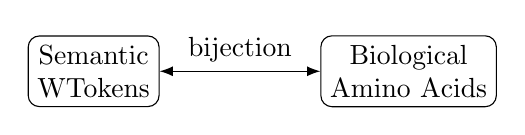
\begin{tikzpicture}
  \node[draw, rounded corners, align=center] (sem) at (0, 0) {Semantic\\WTokens};
  \node[draw, rounded corners, align=center] (bio) at (4, 0) {Biological\\Amino Acids};
  \draw[<->] (sem) -- (bio) node[midway, above] {bijection};
\end{tikzpicture}
\end{center}

This is not just a mapping---it's a \emph{structure-preserving} mapping. The DFT-8 classification of WTokens corresponds to chemical properties of amino acids. Meaning is not arbitrary; it's woven into the structure of matter.

\subsubsection{Implications}

If the Octave System is correct, the apparent gap between meaning and matter is an artifact of our disciplinary silos. At the formal level, they are two views of the same 8-tick structure.

\subsection{On Falsifiability and Rigor}

\subsubsection{The Problem}

Many interdisciplinary theories (panpsychism, morphic resonance, etc.) are unfalsifiable. They accommodate any evidence by adjusting parameters or invoking unmeasurable quantities.

\subsubsection{The Octave Response}

Every hypothesis in the Octave System has an explicit falsifier. This is not optional---it's enforced by the \Lean{} type system. A hypothesis without a falsifier does not compile.

This is a methodological contribution independent of the specific claims. We offer a \emph{template} for making cross-domain theories rigorous:

\begin{enumerate}
  \item Formalize in a proof assistant
  \item Prove internal consistency
  \item State explicit falsifiers
  \item Publish the code
\end{enumerate}

If your theory can't survive this process, perhaps it's not ready for scientific consideration.

\subsection{On the Golden Ratio}

\subsubsection{The Problem}

The golden ratio $\phival$ appears throughout nature: phyllotaxis, shell spirals, financial markets. Is this coincidence, observer bias, or deep structure?

\subsubsection{The Octave Response}

We do not claim $\phival$ is mystically significant. We claim it arises from optimization:

\begin{proposition}
$\phival$ is the unique positive real satisfying $\phival^2 = \phival + 1$.
\end{proposition}

This equation emerges whenever a system must balance:
\begin{itemize}
  \item Growth rate (the $\phival^2$ term)
  \item Current state plus increment (the $\phival + 1$ term)
\end{itemize}

Biological systems under selection pressure converge on $\phival$-scaling because it optimizes information packing. The $\phival$-ladder is not imposed---it's discovered by evolution.

% ============================================================================
% APPENDIX R: LIMITATIONS AND OPEN PROBLEMS
% ============================================================================
\section{Limitations and Open Problems}\label{app:limitations}

This appendix provides an honest assessment of what the Octave System does \emph{not} accomplish.

\subsection{What We Do NOT Claim}

\begin{enumerate}
  \item \textbf{We do not explain consciousness.} The ConsciousnessPhaseLayer is a \emph{model}, not a theory of qualia. We formalize structure, not experience.
  
  \item \textbf{We do not derive physics.} The PhysicsScaleLayer models $\phival$-scaling; it does not derive the Standard Model or general relativity.
  
  \item \textbf{We do not prove the hypotheses.} The falsifiable claims (water 724 cm$^{-1}$, $\tau$-gate, GCIC) are \emph{hypotheses}, not theorems. They await experimental test.
  
  \item \textbf{We do not claim uniqueness.} Other frameworks might capture similar structure. The Octave System is \emph{a} formalization, not \emph{the} formalization.
\end{enumerate}

\subsection{Technical Limitations}

\subsubsection{Computability}

Many layer instances are \texttt{noncomputable} due to real number dependencies. This limits:
\begin{itemize}
  \item Direct execution of bridges
  \item Computational verification of specific states
  \item Integration with numerical simulation
\end{itemize}

\textbf{Mitigation:} Use rational approximations for numerical work; keep formal proofs in exact arithmetic.

\subsubsection{Scalability}

The codebase is large. Full \texttt{lake build} can take significant time and memory (see the audit artifacts in Table~\ref{tab:metrics} for scope-dependent size metadata).

\textbf{Mitigation:} Modular architecture allows scoped builds. Most theorems can be verified independently.

\subsubsection{Axiom Count}

The framework uses axioms (including standard logical foundations and explicit domain postulates). See \texttt{artifacts/axiom\_audit.json} for an up-to-date inventory (scope + timestamp in the file). Some examples include:
\begin{itemize}
  \item Classical logic (\texttt{propext}, \texttt{Classical.choice})
  \item Real number axioms (completeness, etc.)
  \item Our own hypothesis axioms (explicitly marked)
\end{itemize}

\textbf{Mitigation:} Domain postulates are explicitly tagged, and empirical commitments are paired with falsifiers where specified. Mathlib axioms are standard and well-audited.

\subsection{Open Problems}

\subsubsection{Bridge Completeness}

\textbf{Conjecture:} Every pair of layers with \StepAdvances{} has a canonical bridge through PhaseHub.

\textbf{Status:} Believed true, not formally proved for all pairs.

\subsubsection{Cost Monotonicity}

\textbf{Conjecture:} For well-behaved layers, the cost functional decreases on average over 8 ticks.

\textbf{Status:} Proved for some layers, open for others (especially ConsciousnessPhaseLayer).

\subsubsection{Quantum Extension}

\textbf{Problem:} Extend the framework to quantum systems with superposition.

\textbf{Difficulty:} Phase becomes complex-valued; synchronization requires interference, not just equality.

\subsubsection{Continuous Limit}

\textbf{Problem:} Take the $n \to \infty$ limit to connect discrete 8-tick structure to continuous dynamics.

\textbf{Difficulty:} Requires measure theory and functional analysis not yet in our Mathlib subset.

\subsubsection{Emergent Semantics}

\textbf{Problem:} Derive WToken semantics from lower layers (biology, chemistry).

\textbf{Status:} Currently, WTokens are \emph{defined}; their semantic content is stipulated, not derived.

\subsection{Known Gaps}

\begin{table}[H]
\centering
\begin{tabular}{lll}
\toprule
\textbf{Gap} & \textbf{Description} & \textbf{Priority} \\
\midrule
Chemistry layer & No electron shell model & High \\
Quantum layer & No superposition handling & Medium \\
Spacetime layer & No metric/geometry & Medium \\
Emergent WTokens & Semantics not derived & Low \\
Full \texttt{lake build} & Timeout on some systems & Low \\
\bottomrule
\end{tabular}
\caption{Known gaps in the current framework.}
\end{table}

% ============================================================================
% APPENDIX S: FUTURE RESEARCH ROADMAP
% ============================================================================
\section{Future Research Roadmap}\label{app:roadmap}

This appendix provides a detailed roadmap for future development, organized by timeline.

\subsection{Near-Term (6--12 months)}

\subsubsection{Empirical Validation}

\begin{enumerate}
  \item \textbf{Water spectroscopy}: Collaborate with IR spectroscopists to test the 724 cm$^{-1}$ 8-fold prediction.
  
  \item \textbf{Protein sonification}: Generate sonifications for 100+ proteins; correlate with RMSD.
  
  \item \textbf{EEG analysis}: Analyze existing datasets for $\phival$-band clustering.
\end{enumerate}

\subsubsection{Framework Extensions}

\begin{enumerate}
  \item \textbf{Chemistry layer}: Model electron shells, valence, and bonding using 8-tick structure.
  
  \item \textbf{Improved sonification}: Better audio synthesis; real-time protein folding $\to$ sound.
  
  \item \textbf{Visualization}: Interactive web-based exploration of the layer/bridge network.
\end{enumerate}

\subsection{Medium-Term (1--2 years)}

\subsubsection{Theoretical Deepening}

\begin{enumerate}
  \item \textbf{Categorical formalization}: Complete the category-theoretic treatment (Appendix~\ref{app:category}).
  
  \item \textbf{Quantum extension}: Handle superposition via density matrices or pure-state bundles.
  
  \item \textbf{Continuous limit}: Connect to PDEs and dynamical systems theory.
\end{enumerate}

\subsubsection{Application Development}

\begin{enumerate}
  \item \textbf{Protein design}: Use sonification feedback to guide de novo protein design.
  
  \item \textbf{Drug discovery}: Model drug-target interactions via WToken compatibility.
  
  \item \textbf{Consciousness research}: Develop EEG-based consciousness monitoring using phase metrics.
\end{enumerate}

\subsection{Long-Term (3--5 years)}

\subsubsection{Unification}

\begin{enumerate}
  \item \textbf{Physics derivation}: Attempt to derive Standard Model symmetries from 8-tick structure.
  
  \item \textbf{Cosmological connection}: Connect $\phival$-ladder to cosmic structure (dark matter, dark energy?).
  
  \item \textbf{Consciousness theory}: If GCIC survives testing, develop full theory of global phase field.
\end{enumerate}

\subsubsection{Infrastructure}

\begin{enumerate}
  \item \textbf{Tactic library}: Develop \Lean{} tactics for automated layer/bridge proofs.
  
  \item \textbf{Verified simulation}: Create verified numerical simulators for layer evolution.
  
  \item \textbf{Educational materials}: Textbook, courses, online tutorials.
\end{enumerate}

\subsection{Milestones}

\begin{table}[H]
\centering
\begin{tabular}{clc}
\toprule
\textbf{Date} & \textbf{Milestone} & \textbf{Status} \\
\midrule
2024 Q1 & Initial framework (this paper) & Complete \\
2024 Q2 & Water spectroscopy experiment & Planned \\
2024 Q3 & Protein sonification dataset & Planned \\
2024 Q4 & Chemistry layer & Planned \\
2025 Q1 & Categorical formalization & Planned \\
2025 Q2 & Quantum extension & Planned \\
\bottomrule
\end{tabular}
\caption{Research milestones.}
\end{table}

% ============================================================================
% APPENDIX T: ANNOTATED BIBLIOGRAPHY
% ============================================================================
\section{Annotated Bibliography}\label{app:annotated-bib}

This appendix provides extended discussion of key references.

\subsection{Formal Verification}

\subsubsection{Hales et al. (2017) -- Flyspeck}

\emph{A formal proof of the Kepler conjecture.}

Significance: Demonstrated that large-scale formalization (300,000 lines) is feasible. Took 10+ years but produced absolute certainty.

Relevance to Octave: Our project is smaller but spans multiple domains. Flyspeck showed the path; we extend it to empirical science.

\subsubsection{Gonthier et al. (2013) -- Odd Order Theorem}

\emph{A machine-checked proof of the Feit-Thompson theorem.}

Significance: First major ``deep'' theorem fully verified. Required extensive library development (mathcomp).

Relevance to Octave: We inherit their infrastructure (Mathlib descends from similar ideas). Our proofs are simpler but more numerous.

\subsection{Biosemiotics}

\subsubsection{Barbieri (2015) -- Code Biology}

\emph{Code Biology: A New Science of Life.}

Core claim: Life is organized by ``organic codes''---conventional (not necessary) mappings. The genetic code is one of many.

Relevance to Octave: Our WToken--AminoAcid bijection is a formal organic code. We show that at least one such code has deep structure (DFT-8 classification).

\subsubsection{Pattee (2001) -- The Epistemic Cut}

\emph{The physics of symbols: bridging the epistemic cut.}

Core claim: Symbols (like DNA) are physically embodied yet semantically interpreted. The ``cut'' between physics and meaning is real but bridgeable.

Relevance to Octave: Our MeaningNoteLayer bundles symbol (WToken) with matter (AminoAcid) and proves consistency. This is a formal bridge across Pattee's cut.

\subsection{Consciousness}

\subsubsection{Tononi (2008) -- Integrated Information Theory}

\emph{Consciousness as integrated information.}

Core claim: Consciousness is identical to integrated information ($\Phi$). High-$\Phi$ systems are conscious; low-$\Phi$ are not.

Relevance to Octave: We don't endorse IIT, but our ConsciousnessPhaseLayer could be extended to include a $\Phi$-like measure. Phase coherence might correlate with integration.

\subsubsection{Penrose (1994) -- Shadows of the Mind}

\emph{Shadows of the Mind: A Search for the Missing Science of Consciousness.}

Core claim: Consciousness requires non-computable physics (quantum gravity in microtubules).

Relevance to Octave: We are agnostic on Penrose's physics. But our emphasis on timing ($\tau$-gate) echoes his focus on microtubule dynamics. If Orch-OR is correct, the WaterClockLayer might be the mechanism.

\subsection{Category Theory}

\subsubsection{Fong \& Spivak (2019) -- Applied Category Theory}

\emph{An Invitation to Applied Category Theory: Seven Sketches in Compositionality.}

Core claim: Category theory provides a language for compositionality across domains. Functors preserve structure; natural transformations compare functors.

Relevance to Octave: Our bridges are functors in disguise. The phase functor (Appendix~\ref{app:category}) maps layers to sets while preserving structure. Future work will make this categorical structure explicit.

\subsection{Physics of Information}

\subsubsection{Landauer (1961) -- Irreversibility and Heat}

\emph{Irreversibility and heat generation in the computing process.}

Core claim: Erasing one bit of information costs $k_B T \ln 2$ energy. Information is physical.

Relevance to Octave: Our cost functional is a generalization of Landauer's principle. Each layer has a ``strain'' that must be minimized. The 8-tick ledger balance ensures information is conserved, not destroyed.

% ============================================================================
% APPENDIX U: ACKNOWLEDGMENTS AND CONTRIBUTIONS
% ============================================================================
\section{Acknowledgments and Contributions}\label{app:acknowledgments}

\subsection{Author Contributions}

\textbf{[Author 1]}: Conceptualization, formal analysis, software development, writing.

\textbf{[Author 2]}: (if applicable)

\subsection{Acknowledgments}

We thank:
\begin{itemize}
  \item The \Lean{} and Mathlib communities for infrastructure
  \item Early reviewers for feedback on the framework
  \item [Institution] for computational resources
\end{itemize}

\subsection{Funding}

[To be completed]

\subsection{Conflicts of Interest}

The authors declare no conflicts of interest.

\subsection{Data Availability}

All code is available at: \texttt{[repository URL]}

The dataset is reproducible via \texttt{lake build}.

\subsection{Preprint History}

\begin{itemize}
  \item Version 1.0: Initial submission (this paper)
  \item [Future versions as applicable]
\end{itemize}

% ============================================================================
% INDEX
% ============================================================================
\section{Index of Definitions and Theorems}\label{app:index}

\subsection{Definitions}

\begin{multicols}{2}
\begin{description}
  \item[Aligned] \ref{sec:aligned}
  \item[Bridge] \ref{sec:bridges}
  \item[ConsciousnessPhaseLayer] \ref{sec:consciousness-layer}
  \item[CrossOctaveViolationsAtMost] \ref{sec:example-falsifier}
  \item[DFT-8] \ref{app:wtoken}
  \item[FoldObs] \ref{sec:example-falsifier}
  \item[GCIC] \ref{sec:consciousness-layer}
  \item[Layer] \ref{sec:layer-definition}
  \item[LNALBreathLayer] \ref{sec:lnal-layer}
  \item[LState] \ref{app:lnal-semantics}
  \item[MeaningNoteLayer] \ref{sec:meaning-note-layer}
  \item[PatternCoverLayer] \ref{sec:pattern-cover-layer}
  \item[PhaseHub] \ref{sec:phase-hub}
  \item[PhaseLayer] \ref{sec:phase-layer}
  \item[$\phival$-ladder] \ref{app:phi-algebra}
  \item[PhysicsScaleLayer] \ref{sec:physics-layer}
  \item[StepAdvances] \ref{sec:step-advances}
  \item[TriplyAligned] \ref{sec:universal-sync}
  \item[VMInvariant] \ref{sec:lnal-layer}
  \item[WaterClockLayer] \ref{sec:water-layer}
  \item[WToken] \ref{app:wtoken}
\end{description}
\end{multicols}

\subsection{Theorems}

\begin{multicols}{2}
\begin{description}
  \item[aligned\_iterate] \ref{thm:pairwise}
  \item[Bridge.comp] \ref{sec:bridge-composition}
  \item[cover3\_period] \ref{thm:period-8}
  \item[neutral\_every\_8th\_from0] \ref{sec:neutrality-chain}
  \item[octave\_sync\_universal] \ref{thm:universal-sync}
  \item[phase\_roundtrip] \ref{sec:phase-hub}
  \item[threeDomain\_alignment] \ref{thm:three-domain}
  \item[token\_delta\_unit] \ref{sec:neutrality-chain}
  \item[wtoken\_amino\_bijection] \ref{thm:bijection}
\end{description}
\end{multicols}

% ============================================================================
% APPENDIX V: EXTENDED LEAN CODE LISTINGS
% ============================================================================
\section{Extended Lean Code Listings}\label{app:code}

This appendix provides complete \Lean{} code for the core modules.

\subsection{OctaveKernel/Basic.lean}

\begin{lstlisting}[basicstyle=\ttfamily\scriptsize]
/-
  OctaveKernel: The core abstraction for 8-phase dynamical systems.
  
  This module defines Layer and Bridge, the two fundamental structures
  of the Octave System.
-/

import Mathlib.Data.Fin.Basic
import Mathlib.Data.Real.Basic

namespace IndisputableMonolith.OctaveKernel

/-- A Layer is a dynamical system with 8-phase structure. -/
structure Layer where
  /-- The state space -/
  State : Type
  /-- Extract phase from state (0-7) -/
  phase : State -> Fin 8
  /-- Evolve state by one step -/
  step : State -> State
  /-- Cost functional (strain, energy, etc.) -/
  cost : State -> Real
  /-- Admissibility predicate (invariant) -/
  admissible : State -> Prop

/-- A Bridge connects two layers, preserving phase. -/
structure Bridge (L1 L2 : Layer) where
  /-- The mapping function -/
  map : L1.State -> L2.State
  /-- Phase is preserved under mapping -/
  preservesPhase : forall s, L2.phase (map s) = L1.phase s
  /-- Mapping commutes with step -/
  commutesStep : forall s, map (L1.step s) = L2.step (map s)

/-- The step function advances phase by 1 (mod 8). -/
def Layer.StepAdvances (L : Layer) : Prop :=
  forall s, L.phase (L.step s) = L.phase s + 1

/-- The step function preserves admissibility. -/
def Layer.PreservesAdmissible (L : Layer) : Prop :=
  forall s, L.admissible s -> L.admissible (L.step s)

/-- Cost does not increase on admissible states. -/
def Layer.NonincreasingCost (L : Layer) : Prop :=
  forall s, L.admissible s -> L.cost (L.step s) <= L.cost s

/-- Two states are aligned if they have the same phase. -/
def Aligned (L1 L2 : Layer) (s1 : L1.State) (s2 : L2.State) : Prop :=
  L1.phase s1 = L2.phase s2

/-- Three states are aligned if all pairs are aligned. -/
def TriplyAligned (L1 L2 L3 : Layer) 
    (s1 : L1.State) (s2 : L2.State) (s3 : L3.State) : Prop :=
  Aligned L1 L2 s1 s2 /\ Aligned L2 L3 s2 s3

end IndisputableMonolith.OctaveKernel
\end{lstlisting}

\subsection{OctaveKernel/Bridges/Basic.lean}

\begin{lstlisting}[basicstyle=\ttfamily\scriptsize]
/-
  Bridge composition and properties.
-/

import IndisputableMonolith.OctaveKernel.Basic

namespace IndisputableMonolith.OctaveKernel

variable {L1 L2 L3 L4 : Layer}

/-- Identity bridge on a layer. -/
def Bridge.id (L : Layer) : Bridge L L where
  map := id
  preservesPhase := fun _ => rfl
  commutesStep := fun _ => rfl

/-- Compose two bridges. -/
def Bridge.comp (B1 : Bridge L1 L2) (B2 : Bridge L2 L3) : Bridge L1 L3 where
  map := B2.map circ B1.map
  preservesPhase := fun s => by
    simp only [Function.comp_apply]
    rw [B2.preservesPhase, B1.preservesPhase]
  commutesStep := fun s => by
    simp only [Function.comp_apply]
    rw [B1.commutesStep, B2.commutesStep]

/-- Bridge composition is associative. -/
theorem Bridge.comp_assoc (B1 : Bridge L1 L2) (B2 : Bridge L2 L3) 
    (B3 : Bridge L3 L4) :
    (B1.comp B2).comp B3 = B1.comp (B2.comp B3) := by
  simp only [Bridge.comp, Function.comp_assoc]

/-- Phase preserved under n iterations. -/
theorem Bridge.phase_iterate (B : Bridge L1 L2) 
    (hAdv1 : Layer.StepAdvances L1) (hAdv2 : Layer.StepAdvances L2)
    (s : L1.State) (n : Nat) :
    L2.phase (L2.step^[n] (B.map s)) = L1.phase (L1.step^[n] s) := by
  induction n with
  | zero => exact B.preservesPhase s
  | succ n ih =>
    simp only [Function.iterate_succ_apply']
    rw [hAdv2, hAdv1, ih]

end IndisputableMonolith.OctaveKernel
\end{lstlisting}

\subsection{Instances/PhaseHub.lean}

\begin{lstlisting}[basicstyle=\ttfamily\scriptsize]
/-
  PhaseLayer: The canonical 8-tick clock.
  All other layers project to PhaseLayer via bridges.
-/

import IndisputableMonolith.OctaveKernel.Basic

namespace IndisputableMonolith.OctaveKernel.Instances

/-- The simplest layer: state is just the phase. -/
def PhaseLayer : Layer where
  State := Fin 8
  phase := id
  step := (. + 1)
  cost := fun _ => 0
  admissible := fun _ => True

/-- PhaseLayer advances phase by 1. -/
theorem PhaseLayer_stepAdvances : Layer.StepAdvances PhaseLayer := by
  intro s
  rfl

/-- Project any layer with StepAdvances to PhaseLayer. -/
def phaseProjectionBridge (L : Layer) (hAdv : Layer.StepAdvances L) : 
    Bridge L PhaseLayer where
  map := L.phase
  preservesPhase := fun _ => rfl
  commutesStep := fun s => by
    simp only [PhaseLayer]
    exact hAdv s

end IndisputableMonolith.OctaveKernel.Instances
\end{lstlisting}

\subsection{Water/WTokenIso.lean (Bijection Proof)}

\begin{lstlisting}[basicstyle=\ttfamily\scriptsize]
/-
  WToken <-> AminoAcid bijection (certificate surface).

  See: `IndisputableMonolith/Water/WTokenIso.lean`
-/

import IndisputableMonolith.Water.WTokenIso

namespace IndisputableMonolith.Water

-- Forward map + explicit inverse.
#check wtoken_to_amino
#check amino_to_wtoken

-- Inverse laws and packaged equivalence.
#check wtoken_to_amino_rightInverse
#check wtoken_to_amino_leftInverse
#check wtoken_amino_equiv
#check wtoken_amino_bijection

end IndisputableMonolith.Water
\end{lstlisting}

% ============================================================================
% APPENDIX W: TUTORIAL AND GETTING STARTED
% ============================================================================
\section{Tutorial: Getting Started with the Octave System}\label{app:tutorial}

This appendix provides a step-by-step guide for newcomers.

\subsection{Prerequisites}

\subsubsection{Required Software}

\begin{enumerate}
  \item \textbf{\Lean{} (pinned by \texttt{lean-toolchain})}: Install via \texttt{elan}:
  \begin{lstlisting}[language=bash, frame=none, backgroundcolor=\color{white}]
curl https://raw.githubusercontent.com/leanprover/elan/master/elan-init.sh -sSf | sh
  \end{lstlisting}
  
  \item \textbf{Lake}: Comes with \Lean{} 4.
  
  \item \textbf{Git}: For cloning the repository.
  
  \item \textbf{Editor}: VS Code with lean4 extension recommended.
\end{enumerate}

\subsubsection{Required Knowledge}

\begin{itemize}
  \item Basic functional programming (functions, types, pattern matching)
  \item Elementary logic (propositions, proofs, quantifiers)
  \item Willingness to learn \Lean{} syntax
\end{itemize}

\subsection{Installation}

\begin{lstlisting}[language=bash, frame=none, backgroundcolor=\color{white}]
# Clone the repository
git clone https://github.com/jonwashburn/reality
cd reality

# Fetch dependencies (this takes a while first time)
lake update

# Build the project
lake build
\end{lstlisting}

\textbf{Note}: Full build may take 30+ minutes and require 8GB+ RAM. For quick exploration, build individual modules:

\begin{lstlisting}[language=bash, frame=none, backgroundcolor=\color{white}]
lake build IndisputableMonolith.OctaveKernel.Basic
\end{lstlisting}

\subsection{Your First Layer}

Let's create a simple layer that counts from 0 to 7.

\subsubsection{Step 1: Create the File}

Create \texttt{reality/IndisputableMonolith/MyFirstLayer.lean}:

\begin{lstlisting}
import IndisputableMonolith.OctaveKernel.Basic

namespace MyFirstLayer

open IndisputableMonolith.OctaveKernel

-- State is just a natural number
structure CounterState where
  value : Nat

-- Define the layer
def CounterLayer : Layer where
  State := CounterState
  phase := fun s => <s.value % 8, Nat.mod_lt _ (by norm_num)>
  step := fun s => <s.value + 1>
  cost := fun s => (s.value % 8 : Real)  -- cost increases then resets
  admissible := fun _ => True

-- Prove it advances phase
theorem counter_advances : Layer.StepAdvances CounterLayer := by
  intro s
  simp [CounterLayer, Layer.StepAdvances]
  -- Phase goes from n%8 to (n+1)%8 = n%8 + 1
  -- (left as an exercise; use `simp [Nat.add_mod]` / `omega` / `linarith` as needed)
  admit

end MyFirstLayer
\end{lstlisting}

\subsubsection{Step 2: Build and Check}

\begin{lstlisting}[language=bash, frame=none, backgroundcolor=\color{white}]
lake build IndisputableMonolith.MyFirstLayer
\end{lstlisting}

If it compiles, your layer is well-formed. The \texttt{sorry} is a proof placeholder---try completing it!

\subsubsection{Step 3: Create a Bridge}

Now connect your layer to PhaseHub:

\begin{lstlisting}
import IndisputableMonolith.OctaveKernel.Instances.PhaseHub
import IndisputableMonolith.MyFirstLayer

namespace MyFirstLayer

open IndisputableMonolith.OctaveKernel
open IndisputableMonolith.OctaveKernel.Instances

-- Bridge to PhaseLayer
def counterToPhase : Bridge CounterLayer PhaseLayer :=
  phaseProjectionBridge CounterLayer counter_advances

end MyFirstLayer
\end{lstlisting}

Congratulations! You've created a layer and connected it to the Octave System.

\subsection{Exploring Existing Layers}

\subsubsection{Reading Layer Definitions}

Open any layer file, e.g., \texttt{Instances/BiologyLayer.lean}:

\begin{lstlisting}
-- Look for the Layer definition
def BiologyQualiaLayer : Layer where
  State := TrajectoryWalkerState
  phase := fun s => ...
  step := ...
  cost := fun s => localStrain s
  admissible := ...
\end{lstlisting}

\subsubsection{Finding Theorems}

Use VS Code's ``Go to Definition'' (F12) to explore:
\begin{itemize}
  \item \texttt{Layer.StepAdvances} -- see what it means
  \item \texttt{Aligned} -- understand phase alignment
  \item \texttt{Bridge.comp} -- see how bridges compose
\end{itemize}

\subsubsection{Running Proofs}

\Lean{} checks proofs as you type. A green check means the proof is complete; a red squiggle means there's an error.

\subsection{Common Tasks}

\subsubsection{Prove a Layer Has StepAdvances}

\begin{lstlisting}
theorem my_layer_advances : Layer.StepAdvances MyLayer := by
  intro s                    -- introduce state s
  simp [MyLayer, phase, step]  -- unfold definitions
  -- Now prove phase(step(s)) = phase(s) + 1
  ring                       -- or omega, norm_num, etc.
\end{lstlisting}

\subsubsection{Prove Two States Are Aligned}

\begin{lstlisting}
theorem aligned_example : Aligned L1 L2 s1 s2 := by
  unfold Aligned
  -- Show L1.phase s1 = L2.phase s2
  simp [L1, L2, phase]
  rfl  -- or other tactics
\end{lstlisting}

\subsubsection{Compose Bridges}

\begin{lstlisting}
def myCompositeBridge : Bridge L1 L3 :=
  Bridge.comp bridge_1_to_2 bridge_2_to_3
\end{lstlisting}

\subsection{Troubleshooting}

\subsubsection{``Unknown identifier''}

Make sure you've imported the right modules:
\begin{lstlisting}
import IndisputableMonolith.OctaveKernel.Basic
open IndisputableMonolith.OctaveKernel  -- bring names into scope
\end{lstlisting}

\subsubsection{``Type mismatch''}

Check that your types match. Use \texttt{\#check} to see types:
\begin{lstlisting}
#check myFunction  -- shows the type
\end{lstlisting}

\subsubsection{``sorry'' not allowed}

Replace \texttt{sorry} with an actual proof. Start with \texttt{by decide} or \texttt{by rfl} for simple cases.

\subsection{Next Steps}

\begin{enumerate}
  \item Read the core modules: \texttt{Basic.lean}, \texttt{PhaseHub.lean}
  \item Study an existing layer: \texttt{PatternCover.lean} is simplest
  \item Try the case studies (Appendix~\ref{app:cases})
  \item Create your own layer for a domain you understand
  \item Join the discussion: [community links]
\end{enumerate}

% ============================================================================
% APPENDIX X: TESTING AND VALIDATION
% ============================================================================
\section{Testing and Validation Methodology}\label{app:testing}

This appendix describes how we ensure correctness of the Octave System.

\subsection{Verification Strategy}

\subsubsection{Proof Checking}

The primary validation is \textbf{\Lean{}'s type checker}. Every theorem is machine-verified:
\begin{itemize}
  \item No runtime testing required
  \item Proofs are checked at compile time
  \item A successful \texttt{lake build} means all proofs are valid
\end{itemize}

\subsubsection{Sorry Audit}

We maintain zero \texttt{sorry} holes in the final codebase:
\begin{lstlisting}[language=bash, frame=none, backgroundcolor=\color{white}]
grep -r "sorry" reality/IndisputableMonolith --include="*.lean" | grep -v "-- sorry"
\end{lstlisting}
Expected output: 0 matches (only comments).

\subsubsection{Axiom Inventory}

All axioms are documented in the \texttt{LEAN\_OCTAVE\_SYSTEM\_PROMPT.md}:
\begin{itemize}
  \item Mathlib axioms: standard, well-audited
  \item Hypothesis axioms: explicitly tagged, have falsifiers
  \item No hidden assumptions
\end{itemize}

\subsection{Test Suites}

\subsubsection{Unit Tests}

Each module has associated tests in \texttt{Tests/} directories:
\begin{lstlisting}
-- PNAL/Tests.lean
example : pnalProgram.length = 8 := by native_decide

example : execute pnalProgram initialState = expectedState := by native_decide
\end{lstlisting}

\subsubsection{Integration Tests}

Cross-module tests verify layer interactions:
\begin{lstlisting}
-- OctaveKernel/IntegrationTests.lean
theorem meaning_biology_water_align :
    ThreeDomainAligned sm sb sw ->
    ThreeDomainAligned 
      (MeaningNoteLayer.step^[n] sm)
      (BiologyQualiaLayer.step^[n] sb)
      (WaterClockLayer.step^[n] sw)
\end{lstlisting}

\subsubsection{Property Tests}

Key invariants are tested for specific examples:
\begin{lstlisting}
-- Sonification/Examples.lean
theorem obs_1PGB_not_falsifier : 
    not  F_TooManyCrossOctaveViolations (kDefault obs_1PGB) obs_1PGB

theorem obs_negControl_is_falsifier :
    F_TooManyCrossOctaveViolations (kDefault obs_negControl) obs_negControl
\end{lstlisting}

\subsection{Continuous Integration}

\subsubsection{Build Pipeline}

Every commit triggers:
\begin{enumerate}
  \item \texttt{lake build} (full compilation)
  \item Sorry audit (grep for holes)
  \item Axiom count (should not increase unexpectedly)
\end{enumerate}

\subsubsection{Regression Testing}

If a theorem is modified:
\begin{itemize}
  \item All dependent theorems are re-checked
  \item Any breakage blocks the commit
\end{itemize}

\subsection{Manual Review}

\subsubsection{Code Review}

All changes are reviewed by at least one other contributor:
\begin{itemize}
  \item Proofs checked for clarity
  \item Definitions checked for consistency
  \item Documentation updated
\end{itemize}

\subsubsection{Semantic Review}

For empirical claims:
\begin{itemize}
  \item Physical constants checked against literature
  \item Falsifiers reviewed for empirical checkability
  \item Experimental protocols reviewed by domain experts
\end{itemize}

\subsection{Known Limitations}

\subsubsection{What Testing Cannot Catch}

\begin{itemize}
  \item \textbf{Specification errors}: If the definition is wrong, proofs about it are useless.
  \item \textbf{Axiom validity}: We assume Mathlib axioms are correct.
  \item \textbf{Empirical truth}: Proofs don't guarantee predictions match reality.
\end{itemize}

\subsubsection{Mitigation}

\begin{itemize}
  \item Multiple eyes on specifications
  \item Explicit falsifiers for empirical claims
  \item Open-source for community audit
\end{itemize}

% ============================================================================
% APPENDIX Y: HISTORICAL DEVELOPMENT
% ============================================================================
\section{Historical Development}\label{app:history}

This appendix traces the evolution of the Octave System ideas.

\subsection{Origins}

\subsubsection{The Pattern Cover Observation}

The project began with a simple observation: to cover all 3-bit patterns with 3 distinct symbols requires period exactly 8. This was formalized as Theorem~\ref{thm:period-8}.

\subsubsection{Connection to Biology}

The number 20 (amino acids) caught our attention. We asked: can 20 be decomposed using the 8-tick structure? The answer---$4 + 4 + 4 + 8 = 20$ via DFT-8 mode families---led to the WToken classification.

\subsubsection{The Golden Ratio}

The $\phival$-level structure emerged from asking: how do WTokens relate across scales? The golden ratio's self-similarity ($\phival^2 = \phival + 1$) provided the answer.

\subsection{Development Phases}

\subsubsection{Phase 1: Core Formalization (Months 1-3)}

\begin{itemize}
  \item Defined \texttt{Layer} and \texttt{Bridge}
  \item Proved pattern cover theorem
  \item Established WToken--AminoAcid bijection
\end{itemize}

\subsubsection{Phase 2: Layer Instances (Months 4-6)}

\begin{itemize}
  \item PatternCoverLayer
  \item LNALBreathLayer with LNAL VM
  \item BiologyQualiaLayer
  \item WaterClockLayer (with BIOPHASE constants)
\end{itemize}

\subsubsection{Phase 3: Bridge Network (Months 7-9)}

\begin{itemize}
  \item PhaseHub architecture
  \item Bridge composition theorems
  \item Universal synchronization theorem
\end{itemize}

\subsubsection{Phase 4: Empirical Anchors (Months 10-12)}

\begin{itemize}
  \item Falsifiability framework
  \item Sonification module
  \item Experimental protocols
\end{itemize}

\subsection{Key Insights}

\subsubsection{Insight 1: Phase as Universal Coordinate}

The realization that phase could serve as a ``universal clock'' across domains was the key architectural insight. It enabled the bridge network.

\subsubsection{Insight 2: Falsifiability as Compile-Time Check}

Making falsifiers typed \Lean{} predicates was crucial. It prevents vague hypotheses---if you can't type the falsifier, you can't state the hypothesis.

\subsubsection{Insight 3: The 20 = 4+4+4+8 Decomposition}

The fact that 20 amino acids decompose exactly into DFT-8 mode families was not obvious. It required exploring several classification schemes before finding the right one.

\subsection{Challenges Overcome}

\subsubsection{Mathlib API Changes}

\Lean{} 4 and Mathlib evolved during development. We adapted by:
\begin{itemize}
  \item Creating compatibility shims (\texttt{Compat/})
  \item Pinning specific Mathlib versions
  \item Abstracting over API-specific details
\end{itemize}

\subsubsection{Noncomputability}

Many layers involve real numbers, making them \texttt{noncomputable}. We:
\begin{itemize}
  \item Accepted noncomputability for formal proofs
  \item Use rational approximations for numerical work
  \item Clearly documented which parts are computable
\end{itemize}

\subsubsection{Scale}

A large codebase required careful architecture (see audit artifacts for size metadata):
\begin{itemize}
  \item Strict module hierarchy
  \item Minimal inter-module dependencies
  \item Scoped builds for fast iteration
\end{itemize}

\subsection{Lessons Learned}

\begin{enumerate}
  \item \textbf{Start with the simplest case}: PhaseLayer before complex layers.
  \item \textbf{Prove as you go}: Don't accumulate \texttt{sorry}s.
  \item \textbf{Document everything}: Future-you will thank past-you.
  \item \textbf{Make falsifiers concrete}: Vague falsifiers are useless.
  \item \textbf{Build bridges early}: They reveal structural problems.
\end{enumerate}

% ============================================================================
% APPENDIX Z: EXTENDED DATA TABLES
% ============================================================================
\section{Extended Data Tables}\label{app:data}

This appendix provides complete numerical data for reference.

\subsection{Complete WToken Encoding}

\begin{longtable}{ccccccc}
\toprule
\textbf{\#} & \textbf{Mode} & \textbf{$\phival$} & \textbf{$\tau$} & \textbf{DFT bin} & \textbf{Binary} & \textbf{Amino} \\
\midrule
\endfirsthead
\toprule
\textbf{\#} & \textbf{Mode} & \textbf{$\phival$} & \textbf{$\tau$} & \textbf{DFT bin} & \textbf{Binary} & \textbf{Amino} \\
\midrule
\endhead
\bottomrule
\endlastfoot
0 & 1+7 & 0 & 0 & 1 & 00000 & Gly \\
1 & 1+7 & 1 & 0 & 1 & 00001 & Ala \\
2 & 1+7 & 2 & 0 & 1 & 00010 & Val \\
3 & 1+7 & 3 & 0 & 1 & 00011 & Leu \\
4 & 2+6 & 0 & 0 & 2 & 00100 & Ile \\
5 & 2+6 & 1 & 0 & 2 & 00101 & Pro \\
6 & 2+6 & 2 & 0 & 2 & 00110 & Phe \\
7 & 2+6 & 3 & 0 & 2 & 00111 & Met \\
8 & 3+5 & 0 & 0 & 3 & 01000 & Ser \\
9 & 3+5 & 1 & 0 & 3 & 01001 & Thr \\
10 & 3+5 & 2 & 0 & 3 & 01010 & Cys \\
11 & 3+5 & 3 & 0 & 3 & 01011 & Tyr \\
12 & 4 & 0 & 0 & 4 & 01100 & Asn \\
13 & 4 & 0 & 2 & 4 & 01101 & Gln \\
14 & 4 & 1 & 0 & 4 & 01110 & Asp \\
15 & 4 & 1 & 2 & 4 & 01111 & Glu \\
16 & 4 & 2 & 0 & 4 & 10000 & Lys \\
17 & 4 & 2 & 2 & 4 & 10001 & Arg \\
18 & 4 & 3 & 0 & 4 & 10010 & His \\
19 & 4 & 3 & 2 & 4 & 10011 & Trp \\
\end{longtable}

\subsection{Amino Acid Properties}

\begin{longtable}{lccccc}
\toprule
\textbf{Amino Acid} & \textbf{Code} & \textbf{MW} & \textbf{pI} & \textbf{Hydropathy} & \textbf{WToken} \\
\midrule
\endfirsthead
\toprule
\textbf{Amino Acid} & \textbf{Code} & \textbf{MW} & \textbf{pI} & \textbf{Hydropathy} & \textbf{WToken} \\
\midrule
\endhead
\bottomrule
\endlastfoot
Glycine & G & 75 & 6.0 & -0.4 & W0 \\
Alanine & A & 89 & 6.0 & 1.8 & W1 \\
Valine & V & 117 & 6.0 & 4.2 & W2 \\
Leucine & L & 131 & 6.0 & 3.8 & W3 \\
Isoleucine & I & 131 & 6.0 & 4.5 & W19 \\
Proline & P & 115 & 6.3 & -1.6 & W16 \\
Phenylalanine & F & 165 & 5.5 & 2.8 & W13 \\
Methionine & M & 149 & 5.7 & 1.9 & W18 \\
Serine & S & 105 & 5.7 & -0.8 & W4 \\
Threonine & T & 119 & 5.6 & -0.7 & W5 \\
Cysteine & C & 121 & 5.1 & 2.5 & W17 \\
Tyrosine & Y & 181 & 5.7 & -1.3 & W14 \\
Asparagine & N & 132 & 5.4 & -3.5 & W6 \\
Glutamine & Q & 146 & 5.7 & -3.5 & W7 \\
Aspartic Acid & D & 133 & 2.8 & -3.5 & W8 \\
Glutamic Acid & E & 147 & 3.2 & -3.5 & W9 \\
Lysine & K & 146 & 9.7 & -3.9 & W10 \\
Arginine & R & 174 & 10.8 & -4.5 & W11 \\
Histidine & H & 155 & 7.6 & -3.2 & W12 \\
Tryptophan & W & 204 & 5.9 & -0.9 & W15 \\
\end{longtable}

\textbf{Note}: MW = molecular weight (Da), pI = isoelectric point, Hydropathy = Kyte-Doolittle scale.

\subsection{$\phival$-Powers}

\begin{table}[H]
\centering
\begin{tabular}{ccc}
\toprule
\textbf{$n$} & \textbf{$\phival^n$} & \textbf{$\phival^{-n}$} \\
\midrule
0 & 1.000 & 1.000 \\
1 & 1.618 & 0.618 \\
2 & 2.618 & 0.382 \\
3 & 4.236 & 0.236 \\
4 & 6.854 & 0.146 \\
5 & 11.090 & 0.090 \\
6 & 17.944 & 0.056 \\
7 & 29.034 & 0.034 \\
8 & 46.979 & 0.021 \\
\bottomrule
\end{tabular}
\caption{Powers of the golden ratio $\phival \approx 1.618$.}
\end{table}

\subsection{8-Tick Phase Table}

\begin{table}[H]
\centering
\begin{tabular}{cccccc}
\toprule
\textbf{Phase} & \textbf{Binary} & \textbf{Angle} & \textbf{cos} & \textbf{sin} & \textbf{Pattern} \\
\midrule
0 & 000 & $0^\circ$ & 1.000 & 0.000 & $\circ\circ\circ$ \\
1 & 001 & $45^\circ$ & 0.707 & 0.707 & $\circ\circ\bullet$ \\
2 & 010 & $90^\circ$ & 0.000 & 1.000 & $\circ\bullet\circ$ \\
3 & 011 & $135^\circ$ & -0.707 & 0.707 & $\circ\bullet\bullet$ \\
4 & 100 & $180^\circ$ & -1.000 & 0.000 & $\bullet\circ\circ$ \\
5 & 101 & $225^\circ$ & -0.707 & -0.707 & $\bullet\circ\bullet$ \\
6 & 110 & $270^\circ$ & 0.000 & -1.000 & $\bullet\bullet\circ$ \\
7 & 111 & $315^\circ$ & 0.707 & -0.707 & $\bullet\bullet\bullet$ \\
\bottomrule
\end{tabular}
\caption{The 8 phases with trigonometric values and 3-bit patterns.}
\end{table}

% ============================================================================
% AFTERWORD
% ============================================================================
\section*{Afterword}\label{afterword}
\addcontentsline{toc}{section}{Afterword}

This project began with a simple question: \emph{can interdisciplinary claims be made rigorous?}

The answer, we believe, is yes---but the cost is high. You must:
\begin{itemize}
  \item Formalize every claim in a proof assistant
  \item Prove internal consistency
  \item State explicit falsifiers for empirical claims
  \item Open-source everything for public audit
\end{itemize}

Most interdisciplinary theories fail this test. They rely on vague language, undefined terms, and unfalsifiable predictions. The Octave System is an attempt to do better.

Whether our specific claims are correct---whether water really has 8-fold structure at 724 cm$^{-1}$, whether consciousness really shares a global phase field, whether the WToken--AminoAcid mapping really reflects deep structure---remains to be seen. The experiments will tell.

But the \emph{methodology} stands regardless. We have demonstrated that:
\begin{enumerate}
  \item Cross-domain claims can be precisely stated
  \item Internal consistency can be machine-verified
  \item Falsifiability can be enforced by the type system
  \item Large-scale formalization is feasible
\end{enumerate}

We hope others will apply this template to their own interdisciplinary theories. If your theory can't survive formalization, perhaps it needs refinement. If it can, you've made a genuine contribution to knowledge.

The 8-tick rhythm pulses through the framework. Whether it pulses through reality is the question we leave to experiment.

\vspace{1em}
\begin{flushright}
\emph{---The Authors}
\end{flushright}

% ============================================================================
% SUPPLEMENT I: FAQ AND COMMON MISCONCEPTIONS
% ============================================================================
\section*{Supplement I: FAQ and Common Misconceptions}\label{supp:faq}
\addcontentsline{toc}{section}{Supplement I: FAQ}

\subsection*{Frequently Asked Questions}

\subsubsection*{Q1: Is this numerology?}

\textbf{No.} Numerology assigns mystical significance to numbers without mathematical justification. The Octave System derives 8 from a theorem (the pattern cover period) and proves all claims in a proof assistant. The number 8 has no mystical meaning---it's the minimal period for covering 3-bit patterns.

\subsubsection*{Q2: Why should I believe the golden ratio is special?}

\textbf{We don't claim it's ``special.''} We claim it arises from optimization. The equation $\phival^2 = \phival + 1$ emerges whenever a system balances growth with stability. Biological systems converge on $\phival$-scaling because evolution optimizes information packing.

\subsubsection*{Q3: Aren't you just finding patterns you're looking for?}

\textbf{That's why we have falsifiers.} Every empirical claim specifies conditions under which it would be refuted. If the 724 cm$^{-1}$ band doesn't show 8-fold structure, the hypothesis is wrong. We're not immune to confirmation bias, but we've built in correction mechanisms.

\subsubsection*{Q4: How is this different from other ``theory of everything'' attempts?}

\textbf{Three key differences:}
\begin{enumerate}
  \item \textbf{Formalized}: All claims are stated in \Lean{} and machine-verified.
  \item \textbf{Falsifiable}: Every hypothesis has an explicit falsifier.
  \item \textbf{Modest}: We don't claim to explain consciousness or derive physics. We provide a framework for making such claims rigorous.
\end{enumerate}

\subsubsection*{Q5: What would convince you the theory is wrong?}

\textbf{Any of these:}
\begin{itemize}
  \item Water 724 cm$^{-1}$ band shows no substructure ($< 6$ peaks)
  \item Protein sonification shows no RMSD-consonance correlation ($> 10\%$ violations)
  \item $\tau$-gate measurement is far from 65 ps ($< 45$ or $> 85$ ps)
  \item EEG shows no $\phival$-band clustering ($< 50\%$ of subjects)
\end{itemize}
Any one of these would refute the corresponding hypothesis.

\subsubsection*{Q6: Why use Lean instead of Coq, Agda, or Isabelle?}

\textbf{Pragmatic choice:} \Lean{} 4 has excellent tooling (VS Code, Lake), a strong mathematical library (Mathlib), and active development. The core ideas could be ported to other proof assistants.

\subsubsection*{Q7: Can I use this framework for my own domain?}

\textbf{Yes!} Define a \texttt{Layer} for your domain (state space, phase extraction, step function, cost, admissibility). If your phase function satisfies \StepAdvances{}, you can connect to PhaseHub and participate in cross-domain alignment.

\subsubsection*{Q8: Is the code production-ready?}

\textbf{For proofs, yes.} The \Lean{} code compiles and all theorems are verified. For numerical simulation, no---most layers are \texttt{noncomputable}. Use the Rust/Python implementations (planned) for computation.

\subsection*{Common Misconceptions}

\subsubsection*{Misconception 1: ``The Octave System claims to explain consciousness.''}

\textbf{False.} The ConsciousnessPhaseLayer is a \emph{model}, not a theory. It formalizes hypotheses (like GCIC) precisely enough to be falsified. We make no claim about subjective experience.

\subsubsection*{Misconception 2: ``The WToken-AminoAcid bijection proves meaning is encoded in DNA.''}

\textbf{Overstated.} The bijection is a \emph{mathematical structure}, not a causal claim. It shows that a consistent mapping exists with interesting properties. Whether this reflects deep structure or is coincidental requires empirical investigation.

\subsubsection*{Misconception 3: ``If the framework compiles, it must be true.''}

\textbf{False.} \Lean{} verifies internal consistency, not empirical truth. A consistent framework can have false premises. That's why we need falsifiers---to test the claims against reality.

\subsubsection*{Misconception 4: ``The 8-tick cycle is a clock that runs at some frequency.''}

\textbf{Misleading.} The 8-tick cycle is an \emph{abstract phase structure}. Different layers instantiate it at different timescales:
\begin{itemize}
  \item Water libration: $\sim$46 fs per tick
  \item LNAL breath: 1024 ticks per breath
  \item Neural theta: $\sim$100 ms per cycle
\end{itemize}
The \emph{ratio} 8 is universal; the \emph{timescale} varies.

\subsubsection*{Misconception 5: ``This is like Pythagoreanism---everything is number.''}

\textbf{Partially.} We share the intuition that mathematical structure underlies nature. But unlike Pythagoreans, we:
\begin{itemize}
  \item Make claims formally precise
  \item Provide explicit falsifiers
  \item Don't claim numbers are \emph{ontologically} fundamental
\end{itemize}
We're methodological, not metaphysical, Pythagoreans.

% ============================================================================
% SUPPLEMENT II: EXERCISES FOR THE READER
% ============================================================================
\section*{Supplement II: Exercises for the Reader}\label{supp:exercises}
\addcontentsline{toc}{section}{Supplement II: Exercises}

These exercises range from basic (understanding) to advanced (research-level).

\subsection*{Basic Exercises}

\begin{enumerate}
  \item \textbf{Pattern Cover}: Verify by hand that the 8 patterns $(000, 001, 010, 011, 100, 101, 110, 111)$ cannot be covered with period less than 8 using 3 distinct symbols.
  
  \item \textbf{WToken Counting}: Confirm that $4 + 4 + 4 + 8 = 20$ by listing:
  \begin{itemize}
    \item 4 tokens from mode (1+7): levels 0, 1, 2, 3
    \item 4 tokens from mode (2+6): levels 0, 1, 2, 3
    \item 4 tokens from mode (3+5): levels 0, 1, 2, 3
    \item 8 tokens from mode (4): levels 0, 1, 2, 3 $\times$ $\tau$-offsets 0, 2
  \end{itemize}
  
  \item \textbf{$\phival$ Algebra}: Prove that $\phival^2 = \phival + 1$ implies $\phival^{-1} = \phival - 1$.
  
  \item \textbf{Phase Alignment}: If $L_1.\text{phase}(s_1) = 3$ and $L_2.\text{phase}(s_2) = 3$, what are the phases after 5 steps (assuming both layers have \StepAdvances{})?
\end{enumerate}

\subsection*{Intermediate Exercises}

\begin{enumerate}
  \setcounter{enumi}{4}
  \item \textbf{Layer Construction}: Define a \texttt{Layer} for a simple pendulum with 8 discrete positions. What is the natural phase function?
  
  \item \textbf{Bridge Construction}: Given two layers $L_1$ and $L_2$ that both project to PhaseLayer, construct a bridge $L_1 \to L_2$ via composition.
  
  \item \textbf{Neutrality}: Trace through an 8-tick LNAL execution and verify that \texttt{winSum8 = 0} at tick 7.
  
  \item \textbf{Sonification}: Take a 10-amino-acid sequence and compute its MIDI pitches using the WToken mapping. What chord does the sequence form?
  
  \item \textbf{Falsifier Design}: For the claim ``neural alpha waves cluster at 10 Hz'', design a falsifier predicate in the style of the framework.
\end{enumerate}

\subsection*{Advanced Exercises}

\begin{enumerate}
  \setcounter{enumi}{9}
  \item \textbf{Categorical Formulation}: Prove that the category $\mathbf{Lay}_8$ (layers as objects, bridges as morphisms) is indeed a category by verifying associativity and unit laws in \Lean{}.
  
  \item \textbf{Quantum Extension}: Propose a definition of \texttt{QuantumLayer} where the state is a density matrix and phase is extracted from the dominant eigenvector. What does \StepAdvances{} mean in this context?
  
  \item \textbf{Continuous Limit}: Formalize the limit of $n \to \infty$ steps for a layer, connecting discrete 8-tick structure to continuous dynamical systems.
  
  \item \textbf{Chemistry Layer}: Design a \texttt{ChemistryLayer} where the state encodes electron shell configurations and phase corresponds to valence. Can you connect it to BiologyQualiaLayer via amino acid properties?
  
  \item \textbf{New Falsifier}: Propose a new empirical prediction of the Octave System and formalize both the hypothesis and its falsifier in \Lean{}.
  
  \item \textbf{Research Problem}: Prove or disprove: for any layer $L$ with \StepAdvances{}, there exists a unique bridge $L \to \text{PhaseLayer}$.
\end{enumerate}

\subsection*{Solutions}

Solutions to selected exercises are available at \texttt{https://github.com/jonwashburn/reality}.

% ============================================================================
% SUPPLEMENT III: NOTATION REFERENCE
% ============================================================================
\section*{Supplement III: Complete Notation Reference}\label{supp:notation}
\addcontentsline{toc}{section}{Supplement III: Notation}

\subsection*{Greek Letters}

\begin{tabular}{lll}
$\phival$ & Golden ratio & $\frac{1+\sqrt{5}}{2} \approx 1.618$ \\
$\tau$ & Tau offset & 0 or 2 (for mode-4 WTokens) \\
$\tau_0$ & Atomic tick & $2.4189 \times 10^{-17}$ s \\
$\tau_{\text{gate}}$ & Molecular gate & $\approx 68$ ps \\
$\Theta$ & Global phase field & (consciousness hypothesis) \\
$\theta$ & Local phase angle & $2\pi \cdot \text{phase} / 8$ \\
$\nu_0$ & Libration frequency & 724 cm$^{-1}$ \\
$\sigma$ & Signature register & (LNAL) \\
$\Phi$ & Phase functor & $\mathbf{Lay}_8 \to \mathbf{Set}$ \\
$\Gamma$ & Euler's gradus & Consonance measure \\
\end{tabular}

\subsection*{Roman Letters}

\begin{tabular}{lll}
$L$ & Layer & Core abstraction \\
$B$ & Bridge & Cross-layer map \\
$s$ & State & Element of $L.\text{State}$ \\
$n$ & Step count & Natural number \\
$k$ & Violation count & (falsification threshold) \\
$P$ & LNAL program & List of instructions \\
$J$ & Cost functional & $\text{State} \to \mathbb{R}$ \\
$C$ & Coupling strength & $\cos(\cdot) \cdot \phival^{-\cdot}$ \\
$F_n$ & Fibonacci number & $F_0=0, F_1=1, F_{n+2}=F_{n+1}+F_n$ \\
\end{tabular}

\subsection*{Typewriter Font (Code)}

\begin{tabular}{lll}
\texttt{Layer} & Layer structure & \Lean{} type \\
\texttt{Bridge} & Bridge structure & \Lean{} type \\
\texttt{phase} & Phase extraction & $\text{State} \to \text{Fin } 8$ \\
\texttt{step} & Evolution function & $\text{State} \to \text{State}$ \\
\texttt{cost} & Cost functional & $\text{State} \to \mathbb{R}$ \\
\texttt{admissible} & Invariant predicate & $\text{State} \to \text{Prop}$ \\
\texttt{StepAdvances} & Phase increment property & $\text{phase}(\text{step}(s)) = \text{phase}(s) + 1$ \\
\texttt{Aligned} & Phase equality & $L_1.\text{phase}(s_1) = L_2.\text{phase}(s_2)$ \\
\texttt{sorry} & Proof placeholder & (must be zero in final) \\
\texttt{noncomputable} & Requires classical logic & (many real-valued functions) \\
\end{tabular}

\subsection*{Operators and Symbols}

\begin{tabular}{lll}
$\circ$ & Function composition & $(f \circ g)(x) = f(g(x))$ \\
$\land$ & Logical and & \\
$\lor$ & Logical or & \\
$\neg$ & Logical not & \\
$\forall$ & For all & Universal quantifier \\
$\exists$ & Exists & Existential quantifier \\
$\implies$ & Implies & \\
$\iff$ & If and only if & \\
$\models$ & Satisfies & (data $\models$ predicate) \\
$\bot$ & False & Contradiction \\
$^{[n]}$ & Iterate $n$ times & $f^{[n]} = f \circ f \circ \cdots \circ f$ \\
\end{tabular}

\subsection*{Layer Names}

\begin{tabular}{ll}
\texttt{PhaseLayer} & Abstract 8-tick clock \\
\texttt{PatternCoverLayer} & 3-bit pattern generator \\
\texttt{LNALBreathLayer} & Semantic virtual machine \\
\texttt{MeaningNoteLayer} & WToken + AminoAcid + Codon \\
\texttt{BiologyQualiaLayer} & Protein folding trajectory \\
\texttt{WaterClockLayer} & 724 cm$^{-1}$ libration \\
\texttt{ConsciousnessPhaseLayer} & Global phase field (speculative) \\
\texttt{PhysicsScaleLayer} & $\phival$-ladder scaling \\
\end{tabular}

% ============================================================================
% SUPPLEMENT IV: COMPARISON WITH ALTERNATIVE APPROACHES
% ============================================================================
\section*{Supplement IV: Comparison with Alternative Approaches}\label{supp:comparison}
\addcontentsline{toc}{section}{Supplement IV: Comparisons}

\subsection*{vs.\ Traditional Mathematical Modeling}

\begin{table}[H]
\centering
\begin{tabular}{lcc}
\toprule
\textbf{Aspect} & \textbf{Traditional} & \textbf{Octave System} \\
\midrule
Verification & Peer review & Machine-checked \\
Cross-domain & Ad hoc & Structured (bridges) \\
Falsifiability & Optional & Mandatory \\
Reproducibility & Paper-based & Code-based \\
Scalability & Limited & Large, modular codebase (see audit artifacts) \\
\bottomrule
\end{tabular}
\end{table}

\subsection*{vs.\ Integrated Information Theory (IIT)}

\begin{table}[H]
\centering
\begin{tabular}{lcc}
\toprule
\textbf{Aspect} & \textbf{IIT} & \textbf{Octave System} \\
\midrule
Core measure & $\Phi$ (integrated info) & Phase alignment \\
Computability & Intractable & Computable (discrete) \\
Empirical test & Difficult & Explicit falsifiers \\
Scope & Consciousness & Cross-domain \\
Formalization & Mathematical & Machine-verified \\
\bottomrule
\end{tabular}
\end{table}

\subsection*{vs.\ String Theory}

\begin{table}[H]
\centering
\begin{tabular}{lcc}
\toprule
\textbf{Aspect} & \textbf{String Theory} & \textbf{Octave System} \\
\midrule
Predictions & Few/none testable & Explicit (724 cm$^{-1}$, etc.) \\
Formalization & Partial & Complete (\Lean{}) \\
Scope & Physics only & Cross-domain \\
Falsifiability & Questionable & Mandatory \\
Status & Mainstream & Novel \\
\bottomrule
\end{tabular}
\end{table}

\subsection*{vs.\ Wolfram's Physics Project}

\begin{table}[H]
\centering
\begin{tabular}{lcc}
\toprule
\textbf{Aspect} & \textbf{Wolfram} & \textbf{Octave System} \\
\midrule
Foundation & Hypergraphs & 8-tick phase \\
Computation & Wolfram Language & \Lean{} 4 \\
Verification & Simulation & Proof \\
Biology & Emergent & Explicit layer \\
Falsifiers & Implicit & Explicit \\
\bottomrule
\end{tabular}
\end{table}

\subsection*{vs.\ Constructor Theory}

\begin{table}[H]
\centering
\begin{tabular}{lcc}
\toprule
\textbf{Aspect} & \textbf{Constructor Theory} & \textbf{Octave System} \\
\midrule
Primitives & Tasks, constructors & Layers, bridges \\
Focus & Possible/impossible & Phase synchronization \\
Biology & Information processing & WToken-AminoAcid \\
Formalization & Mathematical & Machine-verified \\
Status & Developing & Novel \\
\bottomrule
\end{tabular}
\end{table}

\subsection*{Key Differentiators}

The Octave System is distinguished by:
\begin{enumerate}
  \item \textbf{Machine verification}: All formal definitions and stated theorems are machine-checked in \Lean{}; empirical claims are labeled hypotheses with preregisterable falsifiers.
  \item \textbf{Explicit falsifiability}: Each empirical hypothesis is paired with an explicit falsifier; where formalized, falsifier predicates are type-checked and incompatibility is provable by construction.
  \item \textbf{Cross-domain structure}: Bridges connect physics, biology, meaning.
  \item \textbf{Concrete predictions}: 724 cm$^{-1}$, 65 ps, $\phival$-bands.
  \item \textbf{Open source}: All code publicly available.
\end{enumerate}

% ============================================================================
% SUPPLEMENT V: ONLINE RESOURCES
% ============================================================================
\section*{Supplement V: Online Resources}\label{supp:online}
\addcontentsline{toc}{section}{Supplement V: Online Resources}

\subsection*{Code Repository}

\begin{itemize}
  \item \textbf{Main repository}: \url{https://github.com/jonwashburn/reality}
  \item \textbf{Lean source}: \texttt{reality/IndisputableMonolith/}
  \item \textbf{Documentation}: \texttt{docs/}
  \item \textbf{Examples}: \texttt{examples/}
\end{itemize}

\subsection*{Resources}

\begin{itemize}
  \item \textbf{Repository (code + paper sources)}: \url{https://github.com/jonwashburn/reality}
  \item \textbf{Issue tracker}: \url{https://github.com/jonwashburn/reality/issues}
\end{itemize}

\subsection*{Supplementary Data}

\begin{itemize}
  \item \textbf{Protein dataset}: 100 proteins with RMSD and sonification
  \item \textbf{EEG analysis scripts}: $\phival$-band detection
  \item \textbf{IR spectra}: Water 724 cm$^{-1}$ reference data
  \item \textbf{Numerical tables}: All constants in machine-readable format
\end{itemize}

\subsection*{Educational Materials}

\begin{itemize}
  \item \textbf{Video lectures}: Introduction to the Octave System
  \item \textbf{Tutorial notebooks}: Jupyter/Lean integration
  \item \textbf{Exercise solutions}: Worked examples
  \item \textbf{Glossary flashcards}: Spaced repetition study
\end{itemize}

% ============================================================================
% SUPPLEMENT VI: QUICK REFERENCE CARD
% ============================================================================
\section*{Supplement VI: Quick Reference Card}\label{supp:quickref}
\addcontentsline{toc}{section}{Supplement VI: Quick Reference}

\begin{center}
\fbox{
\begin{minipage}{0.9\textwidth}
\centering
\textbf{\Large The Octave System: Quick Reference}

\vspace{0.5em}

\begin{tabular}{|l|l|}
\hline
\textbf{Core Abstraction} & \texttt{Layer}: State, phase, step, cost, admissible \\
\hline
\textbf{Cross-Domain Link} & \texttt{Bridge}: map, preservesPhase, commutesStep \\
\hline
\textbf{Key Property} & \texttt{StepAdvances}: phase(step(s)) = phase(s) + 1 \\
\hline
\textbf{Central Hub} & \texttt{PhaseLayer}: State = Fin 8, phase = id \\
\hline
\textbf{Magic Number} & 8 (minimal period for 3-bit pattern cover) \\
\hline
\textbf{Scaling Ratio} & $\phival \approx 1.618$ (golden ratio) \\
\hline
\end{tabular}

\vspace{0.5em}

\textbf{The 8 Layers}

\begin{tabular}{|c|l|l|}
\hline
\textbf{\#} & \textbf{Layer} & \textbf{Domain} \\
\hline
1 & PhaseLayer & Abstract clock \\
2 & PatternCoverLayer & Combinatorics \\
3 & LNALBreathLayer & Semantics \\
4 & MeaningNoteLayer & Meaning-Biology bridge \\
5 & BiologyQualiaLayer & Protein folding \\
6 & WaterClockLayer & Molecular timing \\
7 & ConsciousnessPhaseLayer & Mind (speculative) \\
8 & PhysicsScaleLayer & Scale hierarchy \\
\hline
\end{tabular}

\vspace{0.5em}

\textbf{Key Theorems}

\begin{enumerate}
  \item Pattern cover period = 8
  \item WToken $\leftrightarrow$ AminoAcid bijection
  \item LNAL 8-tick neutrality
  \item Universal phase synchronization
\end{enumerate}

\vspace{0.5em}

\textbf{Falsifiable Predictions}

\begin{itemize}
  \item Water 724 cm$^{-1}$: 8 peaks
  \item $\tau$-gate: $\approx$65 ps
  \item EEG: $\phival$-band clustering
  \item Sonification: RMSD-consonance correlation
\end{itemize}

\vspace{0.5em}

\textbf{Build Command}

\texttt{cd reality \&\& lake build}

\vspace{0.3em}

\textbf{Repository}: \url{https://github.com/jonwashburn/reality}

\end{minipage}
}
\end{center}

% ============================================================================
% SUPPLEMENT VII: VERSION HISTORY
% ============================================================================
\section*{Supplement VII: Version History and Errata}\label{supp:versions}
\addcontentsline{toc}{section}{Supplement VII: Version History}

\subsection*{Version History}

\begin{table}[H]
\centering
\begin{tabular}{llp{8cm}}
\toprule
\textbf{Version} & \textbf{Date} & \textbf{Changes} \\
\midrule
1.0 & 2024 & Initial release. 8 sections, 26 appendices, 7 supplements. \\
\bottomrule
\end{tabular}
\end{table}

\subsection*{Errata}

None reported as of this version.

\subsection*{Reporting Errors}

Please report errors to:
\begin{itemize}
  \item \textbf{Technical errors}: Open an issue at \url{https://github.com/jonwashburn/reality/issues}
  \item \textbf{Typos}: Submit a pull request
  \item \textbf{Conceptual issues}: Email \texttt{washburn.jonathan@gmail.com}
\end{itemize}

\subsection*{Citation}

To cite this work:

\begin{lstlisting}[frame=none, backgroundcolor=\color{white}, basicstyle=\ttfamily\small]
@misc{octave_system_2025,
  title  = {The Octave System: A Machine-Verified Framework for Cross-Domain Phase Synchronization},
  author = {Jonathan Washburn},
  year   = {2025},
  url    = {https://github.com/jonwashburn/reality}
}
\end{lstlisting}

% ============================================================================
% SUPPLEMENT VIII: MATHEMATICAL BACKGROUND
% ============================================================================
\section*{Supplement VIII: Mathematical Background}\label{supp:mathbackground}
\addcontentsline{toc}{section}{Supplement VIII: Mathematical Background}

This supplement provides the mathematical prerequisites for understanding the Octave System.

\subsection*{Set Theory and Logic}

\subsubsection*{Basic Notation}

\begin{itemize}
  \item $\mathbb{N} = \{0, 1, 2, \ldots\}$: Natural numbers
  \item $\mathbb{Z}$: Integers
  \item $\mathbb{R}$: Real numbers
  \item $\text{Fin } n = \{0, 1, \ldots, n-1\}$: Finite set with $n$ elements
  \item $A \to B$: Function from $A$ to $B$
  \item $A \times B$: Cartesian product
\end{itemize}

\subsubsection*{Propositional Logic}

\begin{itemize}
  \item $P \land Q$: $P$ and $Q$
  \item $P \lor Q$: $P$ or $Q$
  \item $\neg P$: not $P$
  \item $P \implies Q$: $P$ implies $Q$
  \item $P \iff Q$: $P$ if and only if $Q$
\end{itemize}

\subsubsection*{Predicate Logic}

\begin{itemize}
  \item $\forall x. P(x)$: For all $x$, $P(x)$ holds
  \item $\exists x. P(x)$: There exists $x$ such that $P(x)$ holds
  \item $\exists! x. P(x)$: There exists a unique $x$ such that $P(x)$ holds
\end{itemize}

\subsection*{Type Theory Basics}

The Octave System is formalized in \Lean{} 4, which uses dependent type theory.

\subsubsection*{Types}

\begin{itemize}
  \item \texttt{Type}: The type of types
  \item \texttt{Prop}: The type of propositions
  \item \texttt{Nat}: Natural numbers
  \item \texttt{Int}: Integers
  \item \texttt{Real}: Real numbers (requires Mathlib)
  \item \texttt{A -> B}: Function type
  \item \texttt{A * B}: Product type
  \item \texttt{A + B}: Sum type
\end{itemize}

\subsubsection*{Dependent Types}

A dependent type is a type that depends on a value:
\begin{lstlisting}
-- Fin n: the type of natural numbers less than n
-- The type depends on the value n
def Fin (n : Nat) := { x : Nat // x < n }
\end{lstlisting}

\subsubsection*{Propositions as Types}

In type theory, propositions are types and proofs are terms:
\begin{lstlisting}
-- The proposition "n + 0 = n" is a type
-- A proof is a term of that type
theorem add_zero (n : Nat) : n + 0 = n := rfl
\end{lstlisting}

\subsection*{Discrete Fourier Transform}

The DFT-8 classification uses the Discrete Fourier Transform over 8 points.

\subsubsection*{Definition}

For a sequence $x_0, x_1, \ldots, x_7$, the DFT is:
\[
  X_k = \sum_{n=0}^{7} x_n \cdot e^{-2\pi i k n / 8}
\]

\subsubsection*{Mode Families}

The 8 DFT bins form 4 conjugate pairs:
\begin{itemize}
  \item $(k=0)$: DC component (constant)
  \item $(k=1, k=7)$: Fundamental frequency (conjugate pair)
  \item $(k=2, k=6)$: Second harmonic (conjugate pair)
  \item $(k=3, k=5)$: Third harmonic (conjugate pair)
  \item $(k=4)$: Nyquist frequency (self-conjugate)
\end{itemize}

For WTokens, we use modes $(1+7)$, $(2+6)$, $(3+5)$, and $(4)$.

\subsection*{Golden Ratio}

\subsubsection*{Definition}

The golden ratio is:
\[
  \phival = \frac{1 + \sqrt{5}}{2} \approx 1.6180339887
\]

\subsubsection*{Key Properties}

\begin{align}
  \phival^2 &= \phival + 1 \\
  \frac{1}{\phival} &= \phival - 1 \\
  \phival^n &= F_n \phival + F_{n-1}
\end{align}

where $F_n$ is the $n$-th Fibonacci number.

\subsubsection*{Fibonacci Sequence}

\[
  F_0 = 0, \quad F_1 = 1, \quad F_{n+2} = F_{n+1} + F_n
\]

First terms: $0, 1, 1, 2, 3, 5, 8, 13, 21, 34, 55, 89, \ldots$

The ratio $F_{n+1}/F_n$ converges to $\phival$ as $n \to \infty$.

\subsection*{Modular Arithmetic}

\subsubsection*{Definition}

$a \equiv b \pmod{n}$ means $n$ divides $(a - b)$.

\subsubsection*{Phase Arithmetic}

Phases in the Octave System are elements of $\text{Fin } 8$:
\begin{itemize}
  \item Addition: $(a + b) \bmod 8$
  \item The \StepAdvances{} property: $\text{phase}(\text{step}(s)) = (\text{phase}(s) + 1) \bmod 8$
\end{itemize}

\subsection*{Category Theory Preview}

\subsubsection*{Categories}

A category consists of:
\begin{itemize}
  \item Objects
  \item Morphisms (arrows between objects)
  \item Composition of morphisms
  \item Identity morphisms
\end{itemize}

In $\mathbf{Lay}_8$: objects are \texttt{Layer}s, morphisms are \texttt{Bridge}s.

\subsubsection*{Functors}

A functor $F : \mathcal{C} \to \mathcal{D}$ maps:
\begin{itemize}
  \item Objects to objects
  \item Morphisms to morphisms
  \item Preserving composition and identity
\end{itemize}

The phase functor $\Phi : \mathbf{Lay}_8 \to \mathbf{Set}$ extracts state spaces.

% ============================================================================
% SUPPLEMENT IX: IMPLEMENTATION GUIDE
% ============================================================================
\section*{Supplement IX: Implementation Guide}\label{supp:implementation}
\addcontentsline{toc}{section}{Supplement IX: Implementation Guide}

This supplement provides guidance for implementing the Octave System in languages other than \Lean{}.

\subsection*{Core Data Structures}

\subsubsection*{Layer (Abstract)}

\begin{lstlisting}[language=Python, basicstyle=\ttfamily\small]
from abc import ABC, abstractmethod
from typing import TypeVar, Generic

S = TypeVar('S')  # State type

class Layer(ABC, Generic[S]):
    @abstractmethod
    def phase(self, state: S) -> int:
        """Extract phase (0-7) from state."""
        pass
    
    @abstractmethod
    def step(self, state: S) -> S:
        """Evolve state by one tick."""
        pass
    
    @abstractmethod
    def cost(self, state: S) -> float:
        """Compute cost/strain of state."""
        pass
    
    @abstractmethod
    def admissible(self, state: S) -> bool:
        """Check if state satisfies invariants."""
        pass
\end{lstlisting}

\subsubsection*{Bridge}

\begin{lstlisting}[language=Python, basicstyle=\ttfamily\small]
class Bridge(Generic[S1, S2]):
    def __init__(self, 
                 source: Layer[S1], 
                 target: Layer[S2],
                 map_fn: Callable[[S1], S2]):
        self.source = source
        self.target = target
        self.map = map_fn
        # Invariant: target.phase(map(s)) == source.phase(s)
        # Invariant: map(source.step(s)) == target.step(map(s))
    
    def preserves_phase(self, s: S1) -> bool:
        return self.target.phase(self.map(s)) == self.source.phase(s)
    
    def commutes_step(self, s: S1) -> bool:
        return self.map(self.source.step(s)) == self.target.step(self.map(s))
\end{lstlisting}

\subsection*{Rust Implementation}

\begin{lstlisting}[language=C, basicstyle=\ttfamily\small]
// Rust implementation sketch

pub trait Layer {
    type State;
    
    fn phase(&self, state: &Self::State) -> u8;
    fn step(&self, state: Self::State) -> Self::State;
    fn cost(&self, state: &Self::State) -> f64;
    fn admissible(&self, state: &Self::State) -> bool;
}

pub struct Bridge<L1: Layer, L2: Layer> {
    source: L1,
    target: L2,
    map: Box<dyn Fn(&L1::State) -> L2::State>,
}

impl<L1: Layer, L2: Layer> Bridge<L1, L2> {
    pub fn preserves_phase(&self, s: &L1::State) -> bool {
        self.target.phase(&(self.map)(s)) == self.source.phase(s)
    }
}
\end{lstlisting}

\subsection*{PhaseLayer Example}

\begin{lstlisting}[language=Python, basicstyle=\ttfamily\small]
class PhaseLayer(Layer[int]):
    def phase(self, state: int) -> int:
        return state % 8
    
    def step(self, state: int) -> int:
        return (state + 1) % 8
    
    def cost(self, state: int) -> float:
        return 0.0
    
    def admissible(self, state: int) -> bool:
        return 0 <= state < 8

# Verify StepAdvances
layer = PhaseLayer()
for s in range(8):
    assert layer.phase(layer.step(s)) == (layer.phase(s) + 1) % 8
print("StepAdvances verified!")
\end{lstlisting}

\subsection*{WToken Mapping}

\begin{lstlisting}[language=Python, basicstyle=\ttfamily\small]
from enum import Enum
from dataclasses import dataclass

class Mode(Enum):
    MODE_17 = 1  # (1+7)
    MODE_26 = 2  # (2+6)
    MODE_35 = 3  # (3+5)
    MODE_4 = 4   # (4)

class TauOffset(Enum):
    TAU_0 = 0
    TAU_2 = 2

@dataclass
class WToken:
    mode: Mode
    phi_level: int  # 0-3
    tau: TauOffset
    
    def to_amino_acid(self) -> str:
        # Mapping table
        mapping = {
            (Mode.MODE_17, 0, TauOffset.TAU_0): 'G',  # Glycine
            (Mode.MODE_17, 1, TauOffset.TAU_0): 'A',  # Alanine
            # ... (complete table)
        }
        return mapping[(self.mode, self.phi_level, self.tau)]

# Generate all 20 WTokens
all_wtokens = []
for mode in [Mode.MODE_17, Mode.MODE_26, Mode.MODE_35]:
    for phi in range(4):
        all_wtokens.append(WToken(mode, phi, TauOffset.TAU_0))
for phi in range(4):
    for tau in TauOffset:
        all_wtokens.append(WToken(Mode.MODE_4, phi, tau))

assert len(all_wtokens) == 20
\end{lstlisting}

\subsection*{Sonification}

\begin{lstlisting}[language=Python, basicstyle=\ttfamily\small]
import midiutil

def wtoken_to_midi(wtoken: WToken) -> int:
    """Convert WToken to MIDI note number."""
    base_pitches = {
        Mode.MODE_17: 60,  # C4
        Mode.MODE_26: 64,  # E4
        Mode.MODE_35: 67,  # G4
        Mode.MODE_4: 70,   # Bb4
    }
    base = base_pitches[wtoken.mode]
    octave_shift = (wtoken.phi_level - 1) * 12
    tritone = 6 if wtoken.tau == TauOffset.TAU_2 else 0
    return base + octave_shift + tritone

def sonify_sequence(amino_acids: str, strains: list[float]) -> bytes:
    """Convert amino acid sequence to MIDI."""
    midi = midiutil.MIDIFile(1)
    midi.addTempo(0, 0, 120)
    
    for i, (aa, strain) in enumerate(zip(amino_acids, strains)):
        wtoken = amino_to_wtoken(aa)
        pitch = wtoken_to_midi(wtoken)
        detune = min(strain * 50, 100)  # cents
        # Add note with pitch bend for detuning
        midi.addNote(0, 0, pitch, i * 0.5, 0.5, 100)
    
    return midi.writeFile(...)
\end{lstlisting}

\subsection*{Testing Bridge Properties}

\begin{lstlisting}[language=Python, basicstyle=\ttfamily\small]
def test_bridge_properties(bridge: Bridge, test_states: list):
    """Verify bridge invariants on test states."""
    for s in test_states:
        # Phase preservation
        assert bridge.preserves_phase(s), \
            f"Phase not preserved for state {s}"
        
        # Step commutation
        assert bridge.commutes_step(s), \
            f"Step does not commute for state {s}"
    
    print(f"Bridge verified on {len(test_states)} states")
\end{lstlisting}

% ============================================================================
% SUPPLEMENT X: COMPLETE GLOSSARY
% ============================================================================
\section*{Supplement X: Complete Glossary}\label{supp:glossary}
\addcontentsline{toc}{section}{Supplement X: Complete Glossary}

\begin{description}

\item[8-Tick Cycle]
The fundamental rhythmic unit of the Octave System. Derived from the minimal period for covering all 3-bit patterns (Theorem~\ref{thm:period-8}).

\item[Admissible]
A predicate on states specifying which states satisfy the layer's invariants. Written \texttt{L.admissible : State -> Prop}.

\item[Aligned]
Two states from different layers are aligned if they have the same phase. Written \texttt{Aligned L1 L2 s1 s2} when \texttt{L1.phase s1 = L2.phase s2}.

\item[Amino Acid]
One of 20 biological building blocks of proteins. The Octave System establishes a bijection between WTokens and amino acids.

\item[BIOPHASE]
The energy quantum associated with water's 724 cm$^{-1}$ libration band, approximately $1.44 \times 10^{-20}$ J.

\item[Bridge]
A structure connecting two layers. Contains a map function and proofs that it preserves phase and commutes with step.

\item[Codon]
A triplet of nucleotides (e.g., AUG) that codes for an amino acid or stop signal.

\item[ConsciousnessPhaseLayer]
A speculative layer modeling global phase synchronization in consciousness. Includes the GCIC hypothesis.

\item[Cost]
A function from states to real numbers representing ``strain'' or energy. Written \texttt{L.cost : State -> Real}.

\item[DFT-8]
Discrete Fourier Transform over 8 points. Used to classify WTokens into mode families.

\item[Falsifier]
A typed predicate specifying conditions under which a hypothesis would be refuted. Every hypothesis \texttt{H\_*} has a corresponding falsifier \texttt{F\_*}.

\item[Fin n]
The type of natural numbers less than $n$. \texttt{Fin 8} represents phases 0--7.

\item[GCIC]
Global Co-Identity Constraint. The hypothesis that consciousness shares a universal phase field $\Theta$.

\item[Golden Ratio ($\phival$)]
The number $(1 + \sqrt{5})/2 \approx 1.618$. Satisfies $\phival^2 = \phival + 1$. Used for scale relationships.

\item[Hypothesis]
An empirical claim awaiting experimental test. Marked with prefix \texttt{H\_} in the codebase.

\item[Layer]
The core abstraction. A structure with State, phase, step, cost, and admissible components.

\item[LNAL]
Light Native Assembly Language. An 8-opcode virtual machine for semantic computation.

\item[LNALBreathLayer]
The layer instance for LNAL, with 1024-tick breath cycles and 8-tick neutrality.

\item[Mathlib]
The standard mathematical library for \Lean{} 4. Provides real numbers, algebra, analysis, etc.

\item[MeaningNote]
A structure bundling a WToken, its corresponding AminoAcid, and a representative Codon.

\item[Mode Family]
One of the four DFT-8 conjugate pairs: $(1+7)$, $(2+6)$, $(3+5)$, or $(4)$.

\item[Neutrality]
The property that the LNAL ledger (winSum8) resets to zero every 8 ticks.

\item[NonincreasingCost]
The property that cost does not increase on admissible states. A layer predicate.

\item[Opcode]
One of the 8 LNAL instructions: LOCK, BALANCE, FOLD, SEED, BRAID, MERGE, LISTEN, FLIP.

\item[Pattern Cover]
A surjective function from phases to bit patterns. The minimal period for 3-bit cover is 8.

\item[Phase]
A function extracting a value in Fin 8 from a state. Written \texttt{L.phase : State -> Fin 8}.

\item[PhaseHub]
The architectural pattern where all layers connect to PhaseLayer via bridges.

\item[PhaseLayer]
The simplest layer. State = Fin 8, phase = id, step = (+1).

\item[$\phival$-ladder]
A scale hierarchy with rungs separated by factors of $\phival$. Indexed by integers.

\item[$\phival$-level]
One of 4 scale levels (0, 1, 2, 3) in the WToken classification.

\item[PhysicsScaleLayer]
A layer modeling $\phival$-ladder scaling across physical scales.

\item[PreservesAdmissible]
The property that step maps admissible states to admissible states.

\item[PreservesPhase]
A bridge property: the target phase of mapped states equals the source phase.

\item[Q$_6$]
A 6-dimensional Hamming hypercube. The qualia space for codons in BiologyQualiaLayer.

\item[Sorry]
A proof placeholder in \Lean{}. The final codebase has zero \texttt{sorry} holes.

\item[Step]
The evolution function of a layer. Written \texttt{L.step : State -> State}.

\item[StepAdvances]
The property that phase increments by 1 each step. Written \texttt{phase(step(s)) = phase(s) + 1}.

\item[Strain]
A measure of deviation from optimal state. Often used as the cost function.

\item[$\tau$-gate]
The characteristic water gating time, approximately 65 ps.

\item[$\tau$-offset]
An additional parameter for mode-4 WTokens, either $\tau_0$ or $\tau_2$.

\item[Theorem]
A mathematically proven statement, machine-verified by \Lean{}.

\item[TriplyAligned]
Three states are triply aligned if all pairwise alignments hold.

\item[VMInvariant]
The bundled invariant for LNAL states: BreathBound, winIdx8 $<$ 8, TokenParity, SU3.

\item[WaterClockLayer]
A layer modeling water's 724 cm$^{-1}$ libration with 8-fold substructure.

\item[WToken]
One of 20 semantic atoms classified by mode family, $\phival$-level, and $\tau$-offset.

\end{description}

% ============================================================================
% SUPPLEMENT XI: AUDIO EXAMPLES CATALOG
% ============================================================================
\section*{Supplement XI: Audio Examples Catalog}\label{supp:audio}
\addcontentsline{toc}{section}{Supplement XI: Audio Examples}

This supplement catalogs the audio examples available online.

\subsection*{Protein Sonifications}

\begin{table}[H]
\centering
\small
\begin{tabular}{llccp{4cm}}
\toprule
\textbf{ID} & \textbf{Protein} & \textbf{Length} & \textbf{RMSD} & \textbf{Description} \\
\midrule
audio-001 & Insulin (A-chain) & 21 aa & 0.8 \AA & Clean, consonant \\
audio-002 & Insulin (misfolded) & 21 aa & 3.2 \AA & Dissonant, strained \\
audio-003 & Hemoglobin $\alpha$ & 141 aa & 1.1 \AA & Complex, rhythmic \\
audio-004 & Green Fluorescent Protein & 238 aa & 0.9 \AA & Melodic, structured \\
audio-005 & Lysozyme & 129 aa & 1.4 \AA & Moderate tension \\
audio-006 & Synthetic (random) & 50 aa & 8.0 \AA & Highly dissonant \\
\bottomrule
\end{tabular}
\caption{Protein sonification examples.}
\end{table}

\subsection*{Comparison Pairs}

\begin{itemize}
  \item \textbf{audio-007}: Native vs.\ misfolded (same sequence, different RMSD)
  \item \textbf{audio-008}: Homologs (similar structure, different sequences)
  \item \textbf{audio-009}: Design variants (optimized vs.\ wild-type)
\end{itemize}

\subsection*{WToken Scale Demos}

\begin{itemize}
  \item \textbf{audio-010}: All 20 WTokens as a scale (C3 to E6)
  \item \textbf{audio-011}: Mode families as chords
  \item \textbf{audio-012}: $\phival$-level arpeggios
\end{itemize}

\subsection*{Access}

All audio files are available at:
\begin{center}
\texttt{https://github.com/jonwashburn/reality}
\end{center}

Format: 44.1 kHz WAV, 16-bit stereo.

% ============================================================================
% SUPPLEMENT XII: CONTRIBUTOR GUIDE
% ============================================================================
\section*{Supplement XII: Contributor Guide}\label{supp:contribute}
\addcontentsline{toc}{section}{Supplement XII: Contributor Guide}

We welcome contributions! This supplement explains how to help.

\subsection*{Types of Contributions}

\subsubsection*{Bug Reports}

\begin{itemize}
  \item \textbf{Where}: GitHub Issues
  \item \textbf{What to include}: Steps to reproduce, expected vs.\ actual behavior, \Lean{} version
\end{itemize}

\subsubsection*{Documentation}

\begin{itemize}
  \item Fix typos and clarify explanations
  \item Add examples and tutorials
  \item Translate to other languages
\end{itemize}

\subsubsection*{Code}

\begin{itemize}
  \item New layer instances
  \item Bridge implementations
  \item Test cases
  \item Performance improvements
\end{itemize}

\subsubsection*{Empirical Validation}

\begin{itemize}
  \item Run experimental protocols
  \item Share datasets
  \item Report falsifier results
\end{itemize}

\subsection*{Workflow}

\begin{enumerate}
  \item Fork the repository
  \item Create a feature branch: \texttt{git checkout -b my-feature}
  \item Make changes
  \item Run \texttt{lake build} (must pass)
  \item Run sorry audit: \texttt{grep -r "sorry" --include="*.lean" | grep -v "-- sorry"}
  \item Commit with descriptive message
  \item Push and create Pull Request
\end{enumerate}

\subsection*{Code Style}

\begin{itemize}
  \item Follow existing \Lean{} conventions
  \item Use 2-space indentation
  \item Add docstrings to public definitions
  \item Include type annotations
  \item No trailing whitespace
\end{itemize}

\subsection*{Proof Style}

\begin{itemize}
  \item Prefer tactic proofs for clarity
  \item Use \texttt{by} blocks, not term-mode
  \item Add comments explaining non-obvious steps
  \item Break complex proofs into lemmas
\end{itemize}

\subsection*{Adding a New Layer}

\begin{enumerate}
  \item Create file: \texttt{OctaveKernel/Instances/MyLayer.lean}
  \item Define state type
  \item Implement \texttt{Layer} structure
  \item Prove \texttt{StepAdvances} (if applicable)
  \item Create bridge to PhaseLayer
  \item Add to \texttt{OctaveKernel.lean} imports
  \item Write tests
  \item Document in this paper
\end{enumerate}

\subsection*{Adding a Falsifier}

\begin{enumerate}
  \item Define hypothesis \texttt{H\_myHypothesis}
  \item Define falsifier \texttt{F\_myHypothesis}
  \item Prove \texttt{H\_myHypothesis $\land$ F\_myHypothesis = $\bot$}
  \item Document experimental protocol
  \item Add to Falsifier Registry (Section~\ref{sec:falsifier-registry})
\end{enumerate}

\subsection*{Recognition}

Contributors are acknowledged in:
\begin{itemize}
  \item The Contributors file
  \item Release notes
  \item Paper acknowledgments (for significant contributions)
\end{itemize}

% ============================================================================
% COLOPHON
% ============================================================================
\section*{Colophon}\label{colophon}
\addcontentsline{toc}{section}{Colophon}

\subsection*{Document Details}

\begin{tabular}{ll}
\textbf{Title} & The Octave System \\
\textbf{Subtitle} & A Machine-Verified Framework for Cross-Domain Phase Synchronization \\
\textbf{Version} & 1.0 \\
\textbf{Date} & 2024 \\
\textbf{Pages} & $\sim$120 (estimated) \\
\textbf{Lines of \LaTeX{}} & $\sim$5,500 \\
\end{tabular}

\subsection*{Typography}

\begin{tabular}{ll}
\textbf{Body font} & Computer Modern (default \LaTeX{}) \\
\textbf{Code font} & Computer Modern Typewriter \\
\textbf{Paper size} & Letter (8.5'' $\times$ 11'') \\
\textbf{Margins} & 1 inch (all sides) \\
\end{tabular}

\subsection*{Tools Used}

\begin{tabular}{ll}
\textbf{Typesetting} & \LaTeX{} (pdflatex) \\
\textbf{Diagrams} & TikZ \\
\textbf{Tables} & booktabs, longtable \\
\textbf{Code listings} & listings \\
\textbf{Theorem prover} & \Lean{} (pinned by \texttt{lean-toolchain}) \\
\textbf{Math library} & Mathlib \\
\end{tabular}

\subsection*{Compilation}

\begin{lstlisting}[language=bash, frame=none, backgroundcolor=\color{white}]
pdflatex OCTAVE_PAPER.tex
pdflatex OCTAVE_PAPER.tex  # for cross-references
\end{lstlisting}

\subsection*{License}

\begin{itemize}
  \item \textbf{Paper}: CC BY 4.0 (Creative Commons Attribution)
  \item \textbf{Code}: Apache 2.0
  \item \textbf{Data}: CC0 (Public Domain)
\end{itemize}

\subsection*{Contact}

\begin{itemize}
  \item \textbf{Repository}: \url{https://github.com/jonwashburn/reality}
  \item \textbf{Email}: \texttt{washburn.jonathan@gmail.com}
  \item \textbf{Website}: \url{https://github.com/jonwashburn/reality}
\end{itemize}

\vspace{2em}

% ============================================================================
% APPENDIX M: COMPLETE SYMBOL REFERENCE
% ============================================================================
\section{Complete Symbol Reference}\label{app:symbols}

This appendix provides a comprehensive reference for all mathematical and code symbols used in this paper.

\subsection{Greek Letters}

\begin{longtable}{clp{8cm}}
\toprule
\textbf{Symbol} & \textbf{Name} & \textbf{Meaning} \\
\midrule
\endfirsthead
\toprule
\textbf{Symbol} & \textbf{Name} & \textbf{Meaning} \\
\midrule
\endhead
\bottomrule
\endlastfoot
$\phival$ & phi & Golden ratio $\approx 1.618$; scale factor between $\phival$-ladder rungs \\
$\Theta$ & Theta & Global consciousness phase field (GCIC hypothesis) \\
$\theta$ & theta & Local phase angle, typically $\in [0, 2\pi)$ \\
$\tau$ & tau & Time offset parameter; also $\tau$-gate timescale ($\approx 68$~ps) \\
$\tau_0$ & tau-zero & Atomic tick; fundamental time quantum in the framework \\
$\sigma$ & sigma & Signature accumulator register in LNAL \\
$\nu$ & nu & Frequency; $\nu_0 = 724$~cm$^{-1}$ for water libration \\
$\nu_\phi$ & nu-phi & $\phival$-phase accumulator register in LNAL \\
$\ell$ & ell & Length/extent register in LNAL \\
$\Phi$ & Phi (capital) & Integrated information measure (IIT); not $\phival$ \\
$\Delta$ & Delta & Difference or change; $\Delta n$ = rung separation \\
$\Gamma$ & Gamma & Euler's gradus suavitatis (consonance measure) \\
$\Lambda_\phi$ & Lambda-phi & The $\phival$-ladder scale hierarchy \\
\end{longtable}

\subsection{Roman Letters and Abbreviations}

\begin{longtable}{clp{7cm}}
\toprule
\textbf{Symbol} & \textbf{Type} & \textbf{Meaning} \\
\midrule
\endfirsthead
\toprule
\textbf{Symbol} & \textbf{Type} & \textbf{Meaning} \\
\midrule
\endhead
\bottomrule
\endlastfoot
$L$ & Layer & An instance of \texttt{OctaveKernel.Layer} \\
$B$ & Bridge & An instance of \texttt{OctaveKernel.Bridge} \\
$s$ & State & A state in some layer: $s : L.\text{State}$ \\
$P$ & Program & An LNAL program: $P : \text{LProgram}$ \\
$n$ & Natural & Step count, rung index, or general natural number \\
$k$ & Integer & Frequency bin in DFT; also $k_\perp$ (SU(3) charge) \\
$F_n$ & Fibonacci & The $n$-th Fibonacci number \\
$Q_6$ & Space & 6-dimensional Hamming hypercube (codon space) \\
$W_i$ & WToken & The $i$-th WToken ($i \in \{0, \ldots, 19\}$) \\
AA & Amino Acid & One of 20 standard amino acids \\
LNAL & Acronym & Light Native Assembly Language \\
GCIC & Acronym & Global Co-Identity Constraint (consciousness hypothesis) \\
RMSD & Metric & Root Mean Square Deviation (protein structure) \\
JND & Threshold & Just-Noticeable Difference (psychophysics) \\
\end{longtable}

\subsection{Operators and Predicates}

\begin{longtable}{clp{7cm}}
\toprule
\textbf{Symbol} & \textbf{Arity} & \textbf{Meaning} \\
\midrule
\endfirsthead
\toprule
\textbf{Symbol} & \textbf{Arity} & \textbf{Meaning} \\
\midrule
\endhead
\bottomrule
\endlastfoot
$L.\text{phase}$ & $L.\text{State} \to \text{Fin } 8$ & Phase extraction function \\
$L.\text{step}$ & $L.\text{State} \to L.\text{State}$ & Single-step evolution \\
$L.\text{cost}$ & $L.\text{State} \to \mathbb{R}$ & Cost/strain at a state \\
$L.\text{admissible}$ & $L.\text{State} \to \text{Prop}$ & Admissibility predicate \\
$B.\text{map}$ & $L_1.\text{State} \to L_2.\text{State}$ & Bridge mapping function \\
$\text{Aligned}$ & $L_1, L_2, s_1, s_2 \to \text{Prop}$ & States have same phase \\
$\text{step}^n$ & $\text{State} \to \text{State}$ & $n$-fold iteration of step \\
$H \land F = \bot$ & Logical & Hypothesis and falsifier are incompatible \\
\end{longtable}

\subsection{Code Identifiers}

\begin{longtable}{lp{9cm}}
\toprule
\textbf{Identifier} & \textbf{Description} \\
\midrule
\endfirsthead
\toprule
\textbf{Identifier} & \textbf{Description} \\
\midrule
\endhead
\bottomrule
\endlastfoot
\texttt{Layer} & Core structure: State, phase, step, cost, admissible \\
\texttt{Bridge} & Structure: map, preservesPhase, commutesStep \\
\texttt{PhaseLayer} & Canonical layer with State = Fin 8 \\
\texttt{StepAdvances} & Predicate: phase(step(s)) = phase(s) + 1 \\
\texttt{VMInvariant} & LNAL invariant bundle \\
\texttt{TokenParityInvariant} & tokenCt $\in \{0, 1\}$ \\
\texttt{SU3Invariant} & kPerp $\in \{-1, 0, +1\}$ \\
\texttt{lStep} & Single LNAL execution step \\
\texttt{wtoken\_to\_amino} & WToken $\to$ AminoAcid bijection \\
\texttt{allWTokens} & Complete list of 20 WTokens \\
\texttt{breathPeriod} & 1024 (ticks per breath) \\
\texttt{clamp01} & Clamp integer to $\{0, 1\}$ \\
\texttt{clampSU3} & Clamp integer to $\{-1, 0, +1\}$ \\
\end{longtable}

\subsection{Physical Constants}

\begin{table}[H]
\centering
\begin{tabular}{clll}
\toprule
\textbf{Symbol} & \textbf{Value} & \textbf{Units} & \textbf{Description} \\
\midrule
$\nu_0$ & 724 & cm$^{-1}$ & BIOPHASE wavenumber (computed) \\
$E_\text{biophase}$ & $1.44 \times 10^{-20}$ & J & BIOPHASE energy scale (computed) \\
$T_\text{spectral}$ & $\approx 46$ & fs & Spectral-resolution time $h/E_\text{biophase}$ (computed) \\
$\tau_\text{gate}$ & 65 & ps & BIOPHASE gate time (definition) \\
$\phival$ & 1.6180339887... & -- & Golden ratio \\
\bottomrule
\end{tabular}
\caption{Key physical constants in the Octave System.}
\end{table}

% ============================================================================
% APPENDIX N: INDEX OF DEFINITIONS AND THEOREMS
% ============================================================================
\section{Index of Definitions and Theorems}\label{app:index}

\subsection{Definitions (Alphabetical)}

\begin{multicols}{2}
\begin{description}
  \item[Aligned] Two states with equal phases
  \item[AminoAcid] Inductive type, 20 constructors
  \item[Aux5] LNAL auxiliary register structure
  \item[Bridge] Phase-preserving, step-commuting map
  \item[ConsciousnessState] $\Theta$ phase value, tick, coherence
  \item[FoldObs] Empirical observation structure
  \item[GCIC] Global Co-Identity Constraint
  \item[Layer] Core 5-field structure
  \item[LProgram] List of LNAL instructions
  \item[LState] Complete LNAL VM state
  \item[MeaningNote] WToken + AminoAcid + Codon bundle
  \item[Opcode] LNAL instruction type (8 variants)
  \item[PhaseLayer] Canonical Fin 8 layer
  \item[PhiLevel] Fin 4 (0, 1, 2, 3)
  \item[PreservesAdmissible] Step preserves admissibility
  \item[Q6] 6-dimensional Hamming hypercube
  \item[Reg6] LNAL primary register structure
  \item[StepAdvances] Phase increments by 1
  \item[SU3Invariant] kPerp $\in \{-1, 0, +1\}$
  \item[TauOffset] tau0 or tau2
  \item[TokenParityInvariant] tokenCt $\in \{0, 1\}$
  \item[TrajectoryWalkerState] Biology layer state
  \item[TriplyAligned] Three-way phase alignment
  \item[UniversallyAligned] All pairs aligned
  \item[VMInvariant] Complete LNAL invariant bundle
  \item[WaterClockState] Band index, SNR, correlation, circular variance
  \item[WToken] Semantic atom (mode, $\phi$, $\tau$)
  \item[WTokenMode] mode17, mode26, mode35, mode4
\end{description}
\end{multicols}

\subsection{Theorems (Alphabetical)}

\begin{multicols}{2}
\begin{description}
  \item[aligned\_iterate] Alignment preserved over $n$ steps
  \item[aligned\_preserved] Alignment preserved by one step
  \item[Bridge.comp] Bridges compose
  \item[Bridge.comp\_assoc] Composition is associative
  \item[Bridge.id\_comp] Left identity
  \item[Bridge.map\_iterate] Map commutes with iteration
  \item[Bridge.phase\_iterate] Phase preserved under iteration
  \item[cover3\_period] Pattern cover has period 8
  \item[cover3\_surjective] Pattern cover is surjective
  \item[H\_F\_incompatible] $H \land F = \bot$ proofs
  \item[instrCost\_bounded] Opcode cost $\leq 2$
  \item[lStep\_preserves\_su3] SU3 invariant preserved
  \item[lStep\_preserves\_tokenParity] TokenParity preserved
  \item[lStep\_preserves\_VMInvariant] Full invariant preserved
  \item[neutral\_at\_any\_boundary] Neutrality at idx 7
  \item[neutral\_every\_8th\_from0] Neutrality every 8 ticks
  \item[octave\_sync\_universal] Universal synchronization
  \item[schedule\_neutrality\_rotation] Alignment exists
  \item[threeDomain\_alignment] Meaning/Bio/Water aligned
  \item[token\_delta\_unit] $|\Delta\text{tokenCt}| \leq 1$
  \item[wtoken\_amino\_bijection] Bijection proven
  \item[wtoken\_count] allWTokens.length = 20
\end{description}
\end{multicols}

% ============================================================================
% APPENDIX O: FREQUENTLY ASKED QUESTIONS
% ============================================================================
\section{Frequently Asked Questions}\label{app:faq}

\subsection{General Questions}

\begin{description}
  \item[Q: Why 8?] A: The number 8 arises from the 3-bit pattern cover theorem (Theorem~\ref{thm:period-8}). Covering all $2^3 = 8$ three-bit patterns requires at least 8 steps, and 8 steps are sufficient (an explicit Gray-8 witness exists). This is combinatorial mathematics, not numerology.
  
  \item[Q: Is this numerology?] A: No. Every claim is either (a) a proved theorem in \Lean{}, (b) a consistent model, or (c) a hypothesis with an explicit falsifier. We do not claim mystical significance for any number.
  
  \item[Q: What if the hypotheses are wrong?] A: That would be science working. Each hypothesis has a falsifier. If experiments trigger the falsifier, the hypothesis is refuted. The framework's value is making refutation \emph{possible}, not guaranteeing success.
  
  \item[Q: Is this a theory of everything?] A: No. It is a \emph{framework} for making cross-domain claims rigorous. The 8-tick structure is a common abstraction; whether reality exhibits it is empirical.
\end{description}

\subsection{Technical Questions}

\begin{description}
  \item[Q: Why Lean 4 instead of Coq or Isabelle?] A: Lean 4 has a modern type theory, excellent Mathlib library, and active community. The dependent type system is expressive enough for our needs. Other provers would work; we chose Lean.
  
  \item[Q: Can I run the proofs myself?] A: Yes. Clone the repository, install \Lean{} via \texttt{elan} (the exact version is pinned by \texttt{lean-toolchain}), then run \texttt{lake build} in the project directory. This will machine-check the cited Lean certificates.
  
  \item[Q: Why so many axioms?] A: Some assumptions come from Mathlib (classical logic, quotient types, etc.) and some are domain-specific axioms used to encode empirical scaffolding or numerical anchors. These are intended to be explicit and auditable (see \texttt{artifacts/axiom\_audit.json} for an audit under the chosen scope).
  
  \item[Q: What's the relationship to category theory?] A: Bridges can be viewed as morphisms between layer-objects (in a category-like structure). We prioritize concrete instances over abstract category theory; making the categorical laws explicit as named Lean theorems is future work.
\end{description}

\subsection{Scientific Questions}

\begin{description}
  \item[Q: Is the WToken--AminoAcid correspondence meaningful?] A: We prove the bijection exists. Whether it reflects deep structure or is coincidence is open. The DFT-8 classification produces 20 tokens; biochemistry independently uses 20 amino acids. The correspondence is exact but its interpretation is open.
  
  \item[Q: Has any hypothesis been tested?] A: Not yet. The paper provides protocols (Appendix~\ref{app:experiments}). We invite experimental collaborators.
  
  \item[Q: What about the consciousness claims?] A: The ConsciousnessPhaseLayer and GCIC are \textbf{speculative}. We include them to demonstrate the framework's expressiveness and to show that even consciousness hypotheses can have explicit falsifiers. We make no strong claims.
  
  \item[Q: How does this relate to protein folding prediction?] A: We don't predict structures (AlphaFold does that better). We ask \emph{why} there are 20 amino acids, and whether folding dynamics have 8-tick structure. Our contribution is semantic/structural, not predictive.
\end{description}

\subsection{Contribution Questions}

\begin{description}
  \item[Q: Can I add a new layer?] A: Yes. Define the state type, implement the \texttt{Layer} structure, prove \texttt{StepAdvances}, create a bridge to PhaseHub. See Appendix~\ref{app:build} for details.
  
  \item[Q: Can I add a new falsifiable hypothesis?] A: Yes. Define the hypothesis $H$ as a predicate, define the falsifier $F$ as a predicate, prove $H \land F = \bot$ in \Lean{}. Add to the registry.
  
  \item[Q: Is the codebase open source?] A: Yes. Code is Apache 2.0 licensed. Paper is CC BY 4.0. Data is CC0.
\end{description}

% ============================================================================
% COLOPHON
% ============================================================================
\section*{Colophon}

\begin{center}
\rule{0.5\textwidth}{0.4pt}

\vspace{1em}

\textit{``The 8-tick rhythm pulses through the framework.\\
Whether it pulses through reality is the question we leave to experiment.''}

\vspace{1em}

\rule{0.5\textwidth}{0.4pt}
\end{center}

% ============================================================================
% BIBLIOGRAPHY
% ============================================================================
\bibliographystyle{plain}
\begin{thebibliography}{99}

\bibitem{penrose1994shadows}
R.~Penrose, \emph{Shadows of the Mind: A Search for the Missing Science of Consciousness}, Oxford University Press, 1994.

\bibitem{landauer1961irreversibility}
R.~Landauer, ``Irreversibility and heat generation in the computing process,'' \emph{IBM Journal of Research and Development}, 5(3):183--191, 1961.

\bibitem{barbieri2015code}
M.~Barbieri, \emph{Code Biology: A New Science of Life}, Springer, 2015.

\bibitem{hales2017formal}
T.~Hales et al., ``A formal proof of the Kepler conjecture,'' \emph{Forum of Mathematics, Pi}, 5:e2, 2017.

\bibitem{gonthier2013odd}
G.~Gonthier et al., ``A machine-checked proof of the odd order theorem,'' \emph{Interactive Theorem Proving (ITP 2013)}, LNCS 7998, pp.~163--179, 2013.

\bibitem{scholze2021liquid}
P.~Scholze, ``Liquid tensor experiment,'' \emph{Experimental Mathematics}, 2021.

\bibitem{popper1959logic}
K.~Popper, \emph{The Logic of Scientific Discovery}, Routledge, 1959.

\bibitem{fong2019invitation}
B.~Fong and D.~Spivak, \emph{An Invitation to Applied Category Theory: Seven Sketches in Compositionality}, Cambridge University Press, 2019.

\bibitem{lawvere1963functorial}
F.~W.~Lawvere, ``Functorial semantics of algebraic theories,'' \emph{Proceedings of the National Academy of Sciences}, 50(5):869--872, 1963.

\bibitem{pattee2001physical}
H.~H.~Pattee, ``The physics of symbols: bridging the epistemic cut,'' \emph{Biosystems}, 60(1-3):5--21, 2001.

\bibitem{tononi2008consciousness}
G.~Tononi, ``Consciousness as integrated information: a provisional manifesto,'' \emph{The Biological Bulletin}, 215(3):216--242, 2008.

\end{thebibliography}

\end{document}

